\documentclass[12pt,a4paper,twoside,openright]{report}

\usepackage[utf8]{inputenc}
\usepackage[greek,english]{babel}
\usepackage[LGR,T1]{fontenc}
\usepackage{lmodern}
\usepackage{substitutefont}
\substitutefont{LGR}{\rmdefault}{artemisia}
\usepackage{graphicx}
\usepackage{geometry}
\geometry{a4paper, margin=2.5cm}
\usepackage{xcolor}
\definecolor{tucred}{RGB}{167, 37, 63}
\definecolor{tucdarkred}{RGB}{115, 25, 44}
\usepackage{amsmath}
\usepackage{amssymb}
\usepackage{booktabs}
\usepackage{multirow}
\usepackage{float}
\usepackage{tikz}
\usetikzlibrary{shapes.geometric, arrows.meta, positioning, calc}
\usepackage{hyperref}
\usepackage{cite}
\usepackage{titlesec}
\titleformat{\section}{\Large\bfseries\raggedright}{\thesection}{1em}{}
\titleformat{\subsection}{\large\bfseries\raggedright}{\thesubsection}{1em}{}
\usepackage{setspace}
\usepackage[protrusion=true,expansion=false]{microtype}
\frenchspacing
\usepackage{fancyhdr}
\pagestyle{fancy}
\setlength{\headheight}{14.5pt}
\fancyhf{}
\fancyfoot[C]{\thepage}
\fancyhead[L]{\leftmark}

\usepackage[ruled,vlined,linesnumbered]{algorithm2e}

% Clear headers and footers on empty pages generated by \cleardoublepage
\makeatletter
\def\cleardoublepage{\clearpage\if@twoside \ifodd\c@page\else
  \hbox{}
  \thispagestyle{empty}
  \newpage
  \if@twocolumn\hbox{}\newpage\fi\fi\fi}
\makeatother

\hypersetup{
    colorlinks=true,
    linkcolor=tucdarkred,
    linktoc=all,
    filecolor=magenta,      
    urlcolor=blue,
    citecolor=black,
}

\begin{document}

% ==============================================================================
% ORIGINAL TITLE PAGE (BACKUP)
% ==============================================================================
% \begin{titlepage}
%     \centering
%     
\includegraphics[width=0.3\textwidth]{tuc_logo.png}
%     \vspace{1cm}
%     
%     {\scshape\LARGE \href{https://www.tuc.gr}{\color{black}Technical University of Crete} \par}
%     \vspace{0.5cm}
%     {\scshape\Large \href{https://www.ece.tuc.gr}{\color{black}School of Electrical \& Computer Engineering} \par}
%     \vspace{1cm}
%     
%     {\scshape\Large Diploma Thesis \par}
%     \vspace{1cm}
%     
%     {\LARGE\bfseries Investigating the Applicability of Federated Dynamic Averaging in Federated Low-Rank Adaptation Architectures\par}
%     \vspace{1cm}
%     
%     \textbf{Author:}\\
%     {\Large\itshape Asterinos Karalis \par}
%     \vspace{1cm}
%     
%     \textbf{Thesis Committee:}\\
%     Prof. Vasilis Samoladas (Supervisor)\\
%     \href{http://www.softnet.tuc.gr/~adeli/}{\color{black}Prof. Antonios Deligiannakis}\\
%     \href{https://minosng.github.io/}{\color{black}Prof. Minos Garofalakis}
%     
%     \vfill
%     
%     A thesis submitted in partial fulfillment of the requirements\\
%     for the degree of Diploma in Electrical and Computer Engineering
%     
%     \vspace{1.5cm}
%     
%     {\large September, 2026 \par}
%     \thispagestyle{empty}
% \end{titlepage}
% \cleardoublepage
% ==============================================================================

\begin{titlepage}
    \vspace*{-1.2cm}
    \centering
    
\includegraphics[width=0.38\textwidth]{tuc_logo.png}
    \vspace{0.6cm}
    
    {\scshape\huge \href{https://www.tuc.gr}{\color{tucred}Technical University of Crete} \par}
    \vspace{0.4cm}
    {\scshape\fontsize{18.5pt}{22pt}\selectfont \href{https://www.ece.tuc.gr}{\color{black}School of Electrical \& Computer Engineering} \par}
    \vspace{0.8cm}
    
    {\scshape\huge Diploma Thesis \par}
    \vspace{0.6cm}
    
    {\color{tucred}\rule{\textwidth}{0.8pt}}\par
    \vspace{0.6cm}
    
    {\LARGE\bfseries Investigating the Applicability of Federated Dynamic Averaging in Federated Low-Rank Adaptation Architectures\par}
    
    \vspace{0.6cm}
    {\color{tucred}\rule{\textwidth}{0.8pt}}\par
    \vspace{1.5cm}
    
    \noindent
    \begin{minipage}[t]{0.48\textwidth}
        \raggedright
        \textbf{Author:}\\[0.3em]
        {\large Asterinos Karalis \par}
    \end{minipage}%
    \hfill
    \begin{minipage}[t]{0.48\textwidth}
        \raggedleft
        \textbf{Thesis Committee:}\\[0.3em]
        {\large \href{https://www.tuc.gr/el/index.php?id=5639&&tx_tuclabspersonnel_pi3\%5Bpersonid\%5D=361}{\color{black}Assoc. Prof. Vasilis Samoladas} (Supervisor)\\}
        {\large \href{http://www.softnet.tuc.gr/~adeli/}{\color{black}Prof. Antonios Deligiannakis}\\}
        {\large \href{https://minosng.github.io/}{\color{black}Prof. Minos Garofalakis}}
    \end{minipage}
    
    \vfill
    
    A thesis submitted in partial fulfillment of the requirements\\
    for the degree of Diploma in Electrical and Computer Engineering
    
    \vspace{1.5cm}
    
    {\large November 2026 \par}
    \thispagestyle{empty}
\end{titlepage}
\cleardoublepage

\pagenumbering{roman}

\singlespacing

% Frontmatter
\chapter*{Abstract}
\addcontentsline{toc}{chapter}{Abstract}

Federated Learning has established itself as a foundational paradigm for privacy-preserving collaborative model training across decentralized data sources. However, scaling modern foundation models to billions of parameters exposes a critical dual bottleneck in federated optimization: an excessive \emph{spatial} communication overhead from transmitting high-dimensional parameter updates, and an inefficient \emph{temporal} communication pattern imposed by rigid, fixed-interval synchronization schedules. Parameter-efficient fine-tuning methods such as Low-Rank Adaptation address the spatial dimension by decomposing updates into compact low-rank factors. Yet, naively applying Low-Rank Adaptation in federated environments introduces a fundamental structural inconsistency: independent averaging of constituent low-rank matrices fails to reconstruct the true global update due to the non-commutativity of matrix multiplication. Furthermore, existing federated Low-Rank Adaptation variants remain temporally inefficient by relying on static synchronization frequencies agnostic to local training dynamics.

To address both dimensions simultaneously, this thesis investigates combining Federated Dynamic Averaging with federated low-rank adaptation. Specifically, we develop and formulate FDA-RoLoRA, an algorithmic formulation that pairs dynamic, variance-driven averaging with Robust Low-Rank Adaptation. This method eliminates the bilinear aggregation inconsistency through alternating updates between down-projection and up-projection matrices, while dynamically regulating synchronization frequency via decoupled, dynamically updated per-matrix variance thresholds. We evaluate the proposed framework on the General Language Understanding Evaluation (GLUE) benchmark using the roberta-base model.






\cleardoublepage

\chapter*{Acknowledgements}
\addcontentsline{toc}{chapter}{Acknowledgements}

\vspace{0.3cm}

First and foremost, I would like to express my sincere gratitude to my supervisor, Assoc. Prof. Vasilis Samoladas, for his continuous guidance, insightful advice, and constructive feedback throughout this thesis. His courses in Distributed Systems and Machine Learning Systems were pivotal during my studies, providing the core foundation for this research.

I extend my sincere appreciation to the examination committee members, Prof. Antonios Deligiannakis and Prof. Minos Garofalakis, for their time, thorough review, and valuable observations on this work.

I am equally grateful to my friends for their support, encouragement, and the unforgettable moments shared throughout our university years in Chania.

Finally, I dedicate this thesis to my family. Their unconditional love, patience, and continuous support have been my strongest anchor throughout every step of this journey.


\cleardoublepage

\tableofcontents
\cleardoublepage

\phantomsection
\addcontentsline{toc}{chapter}{List of Figures}
\listoffigures
\cleardoublepage

\phantomsection
\addcontentsline{toc}{chapter}{List of Tables}
\listoftables
\cleardoublepage

\phantomsection
\addcontentsline{toc}{chapter}{List of Algorithms}
\listofalgorithms
\cleardoublepage

\chapter*{List of Abbreviations}
\addcontentsline{toc}{chapter}{List of Abbreviations}

{\color{tucdarkred}
\begin{tabular}{@{}ll@{}}
\textbf{Abbreviation} & \textbf{Description} \\[6pt]
\textbf{EMA}          & Exponential Moving Average \\
\textbf{FDA}          & Federated Dynamic Averaging \\
\textbf{FDA-RoLoRA}   & Federated Dynamic Averaging with Robust Low-Rank Adaptation \\
\textbf{FedAvg}       & Federated Averaging \\
\textbf{FedLoRA}      & Federated Low-Rank Adaptation \\
\textbf{FedOpt}       & Federated Optimization \\
\textbf{FFA-LoRA}     & Federated Freeze-A Low-Rank Adaptation \\
\textbf{FL}           & Federated Learning \\
\textbf{FLoRA}        & Heterogeneous Federated Low-Rank Adaptation \\
\textbf{GLUE}         & General Language Understanding Evaluation \\
\textbf{IID}          & Independent and Identically Distributed \\
\textbf{LLM}          & Large Language Model \\
\textbf{LoRA}         & Low-Rank Adaptation \\
\textbf{MNLI}         & Multi-Genre Natural Language Inference \\
\textbf{PEFT}         & Parameter-Efficient Fine-Tuning \\
\textbf{QNLI}         & Question Natural Language Inference \\
\textbf{QQP}          & Quora Question Pairs \\
\textbf{RoLoRA}       & Robust Low-Rank Adaptation \\
\textbf{SGD}          & Stochastic Gradient Descent \\
\textbf{SLoRA}        & Sparse Low-Rank Adaptation \\
\textbf{SMA}          & Simple Moving Average \\
\textbf{SST-2}        & Stanford Sentiment Treebank (Binary) \\
\textbf{SVD}          & Singular Value Decomposition \\
\end{tabular}
}

\cleardoublepage

\pagenumbering{arabic}

% Main Chapters
\chapter{Introduction}
\label{chap:intro}
Federated Learning (FL) \cite{kairouz2021advances, mcmahan2017communication} has established itself as the leading paradigm for training machine learning models across decentralized data owners without requiring the centralization of raw user data. By enabling participating nodes---ranging from resource-constrained edge devices to institutional data silos such as hospitals and financial institutions---to compute updates locally and share only parameter tensors with a coordinating server, FL enables collaborative optimization while respecting data privacy regulations (e.g., GDPR, HIPAA) and proprietary commercial boundaries.

However, the iterative nature of federated optimization introduces a severe communication bottleneck. Historically, research in distributed machine learning has tackled this challenge primarily through temporal and algorithmic mechanisms designed for standard neural architectures. Yet, the recent paradigm shift toward massive foundation models has created an entirely new spatial crisis, rendering classical federated optimization techniques insufficient on their own.

\section{Federated Learning and Optimization}
\label{sec:intro-fl-opt}
In canonical federated optimization, the central communication bottleneck is dictated by the synchronization frequency between clients and the central server. The foundational Federated Averaging (FedAvg) algorithm \cite{mcmahan2017communication} coordinates training by having clients execute a fixed, predetermined number of local stochastic gradient descent (SGD) epochs ($E$) before transmitting their updated parameter vectors to the server for aggregation. 

While conceptually simple, rigid synchronization cadences suffer from fundamental inefficiencies under real-world conditions:
\begin{itemize}
    \item \textbf{Statistical Heterogeneity and Client Drift:} In decentralized environments, local client datasets are inherently non-identically and independently distributed (non-IID) \cite{li2020federated, karimireddy2020scaffold}. When clients execute multiple uncoordinated local epochs, their local models drift toward local empirical minima that diverge sharply from the global optimization trajectory.
    \item \textbf{Temporal Redundancy:} Enforcing a static schedule remains blind to actual client convergence. In phases where local updates are minor or homogeneous, transmitting parameters after every fixed interval wastes critical network bandwidth on redundant updates. Conversely, when clients diverge rapidly, static schedules delay aggregation, exacerbating model divergence.
\end{itemize}

To improve federated optimization, adaptive server-side optimizers were introduced under the Federated Optimization (FedOpt) framework \cite{reddi2021adaptive}. By interpreting aggregated client updates as pseudo-gradients and applying momentum-based tracking (such as FedAdam and FedYogi), FedOpt stabilizes the global optimization trajectory against client drift. 

Subsequently, to resolve the rigid cadence of static rounds, Federated Dynamic Averaging (FDA-Opt) \cite{theologitis2025fda, frangias2023federated} introduced variance-driven dynamic synchronization. Rather than synchronizing after fixed epochs, FDA-Opt continuously monitors the pairwise drift and variance across participating clients. Synchronization is triggered dynamically only when parameter variance breaches an adaptive drift threshold ($\theta$). By synchronizing strictly when mathematically necessary, FDA-Opt proved that dynamic temporal throttling can dramatically reduce total communication rounds without sacrificing final accuracy.

Crucially, however, FedAvg, FedOpt, and FDA-Opt all share a common architectural assumption: \emph{the transmission and synchronization of full-rank model parameter vectors}.

\section{Foundation Models and Parameter-Efficient Fine-Tuning}
\label{sec:intro-foundation-peft}
In recent years, the machine learning landscape has undergone an unprecedented transformation driven by large-scale pre-trained foundation models and Large Language Models (LLMs) scaling to billions of parameters \cite{brown2020language, bommasani2021opportunities}. Adapting these foundation models to specialized domain tasks (e.g., clinical diagnosis, legal discovery, financial fraud detection) is of paramount importance.

Yet, this shift in model scale fundamentally breaks the physical viability of full-parameter federated learning:
\begin{itemize}
    \item Synchronizing a modern 7-billion parameter language model (such as LLaMA-2-7B \cite{touvron2023llama}) in 16-bit half-precision requires transmitting approximately \textbf{14 Gigabytes} of parameter data per client per round.
    \item In a cross-silo federated setting with 50 participating institutions over a modest horizon of 100 communication rounds, total network transfer exceeds \textbf{70 Terabytes}---an operational volume that is wholly intractable over standard wide-area network (WAN) connections.
    \item Even for moderately sized encoders such as RoBERTa-Large \cite{liu2019roberta} (355M parameters), a single full-parameter round requires $\sim$1.4 GB per client, swamping edge up-links.
\end{itemize}

To overcome this spatial bottleneck, Parameter-Efficient Fine-Tuning (PEFT) has emerged as an indispensable methodology. Among PEFT strategies, Low-Rank Adaptation (LoRA) \cite{hu2022lora} has become the de facto standard. LoRA keeps the large pre-trained weight matrix $W_0 \in \mathbb{R}^{d \times k}$ frozen, and factorizes task-specific parameter updates into two low-rank matrices:
\begin{equation}
    W = W_0 + \Delta W = W_0 + \frac{\alpha}{r} B A
    \label{eq:intro_lora_decomposition}
\end{equation}
where $A \in \mathbb{R}^{d \times r}$ denotes the down-projection matrix, $B \in \mathbb{R}^{r \times k}$ denotes the up-projection matrix, and the rank $r \ll \min(d, k)$ (typically $r \in \{4, 8, 16\}$). Because only $A$ and $B$ are updated during training, LoRA compresses the volume of communicated parameters by over $99\%$, providing a powerful spatial solution for edge and silo environments.

\section{Aggregation Inconsistency in Federated LoRA}
\label{sec:intro-inconsistency}
Given the spatial efficacy of LoRA, directly integrating low-rank adapters into federated learning---often termed Federated LoRA (FedLoRA) or FedIT \cite{yang2025federated, zhang2023towards}---appears to be a natural path forward. In naive FedLoRA, each client $i \in \{1, \dots, N\}$ initializes identical low-rank matrices, computes local gradient updates on private data, and transmits only its trained adapter matrices $A_i$ and $B_i$ to the central server.

However, aggregating independently trained low-rank factors via standard FedAvg introduces a fatal mathematical failure mode: \emph{LoRA aggregation inconsistency} (or aggregation discordance) \cite{yang2025federated}. Because matrix multiplication is non-linear and non-commutative, averaging the factor matrices independently across clients fails to reconstruct the true average of their composite weight updates:
\begin{equation}
    \frac{1}{N}\sum_{i=1}^{N} (B_i A_i) \neq \left(\frac{1}{N}\sum_{i=1}^{N} B_i\right)\left(\frac{1}{N}\sum_{i=1}^{N} A_i\right)
    \label{eq:intro_inconsistency}
\end{equation}

When the central server independently averages $A_i$ and $B_i$, the composite product of the averaged matrices generates cross-term interference vectors that do not exist in any client's local optimization trajectory. This bilinear distortion collapses the low-rank representation, induces severe gradient cancellation, and destabilizes global convergence, frequently causing fine-tuning to perform worse than static heuristics or simple localized training.

\section{Robust Low-Rank Adaptation}
\label{sec:intro-rolora}
To resolve this bilinear aggregation discordance, several structural workarounds have been explored in recent literature:
\begin{itemize}
    \item \textbf{Full Weight Reconstruction:} Clients could theoretically reconstruct the dense update $\Delta W_i = \frac{\alpha}{r} B_i A_i$ before transmission, or the server could perform Singular Value Decomposition (SVD) on the aggregated full matrix \cite{yang2025federated}. However, this completely nullifies the spatial communication savings of LoRA and imposes prohibitive computational overhead.
    \item \textbf{Static Down-Projection Freezing (FFA-LoRA):} FFA-LoRA \cite{sun2024improving} permanently freezes the down-projection matrix $A$ as a random projection across all clients, allowing clients to train and transmit only the up-projection matrix $B$. While this linearizes aggregation ($\frac{1}{N}\sum A B_i = A \frac{1}{N}\sum B_i$), permanently freezing half of the parameter degrees of freedom severely compromises adapter capacity and expressive power.
    \item \textbf{Heterogeneous Rank Assembly (FLoRA):} FLoRA \cite{wang2024flora} attempts to support variable client ranks by stacking updates, but still incurs heavy reconstruction overhead on the aggregation server.
\end{itemize}

A decisive breakthrough resolving this dilemma without sacrificing model expressiveness is \textbf{Robust Low-Rank Adaptation (RoLoRA)} \cite{chen2025robust}. RoLoRA adopts an \emph{alternating coordinate optimization} strategy. Instead of updating both factor matrices simultaneously, training alternates in structured multi-round blocks:
\begin{enumerate}
    \item In Phase A, matrix $A$ is frozen globally across all clients, and only matrix $B$ is trained locally and aggregated.
    \item In Phase B, the updated matrix $B$ is frozen globally across all clients, and only matrix $A$ is trained locally and aggregated.
\end{enumerate}

Because one coordinate factor is held globally identical across all clients during any given aggregation phase, the averaging operation becomes strictly linear:
\begin{equation}
    \frac{1}{N} \sum_{i=1}^{N} (B_i A_{\text{frozen}}) = \left( \frac{1}{N} \sum_{i=1}^{N} B_i \right) A_{\text{frozen}}
    \label{eq:intro_rolora_linearity}
\end{equation}
By toggling the active subspace over alternating cycles, RoLoRA preserves the full representational rank and expressive capacity of standard LoRA while restoring mathematically exact federated averaging.

\section{Proposed Method: FDA-RoLoRA}
\label{sec:intro-fdarolora}
With RoLoRA restoring mathematical linearity to federated low-rank aggregation, an extraordinary scientific opportunity emerges: \emph{Can we now unify the temporal adaptivity of Federated Dynamic Averaging with the spatial efficiency of alternating low-rank adaptation?}

While RoLoRA successfully solves the spatial aggregation inconsistency, existing RoLoRA formulations remain shackled to \textbf{rigid, predetermined synchronization cadences} (fixed local steps or epochs). Clients must synchronize their active matrix after arbitrary epoch boundaries, inheriting all the temporal redundancies and drift penalties of classical FedAvg.

Conversely, while FDA-Opt \cite{theologitis2025fda} pioneered variance-driven dynamic synchronization, it was formulated exclusively for monolithic full-rank neural networks. Simply applying FDA-Opt directly to RoLoRA is impossible due to three fundamental obstacles:
\begin{enumerate}
    \item \textbf{Asymmetric Coordinate Geometries:} The down-projection matrix $A \in \mathbb{R}^{r \times d_{\text{in}}}$ and up-projection matrix $B \in \mathbb{R}^{d_{\text{out}} \times r}$ fulfill entirely different functional roles (compression vs. expansion). Furthermore, standard initialization schemes ($A \sim \mathcal{N}(0, \sigma^2)$ and $B = 0$) create highly divergent gradient dynamics, spectral velocities, and parameter drift magnitudes. A single scalar threshold cannot govern both spaces.
    \item \textbf{Subspace Coordinate Variance:} If client variance were computed by projecting updates back to full-rank matrices ($\Delta W = \frac{\alpha}{r} BA$), all computational and memory benefits of PEFT would be lost. Client drift must be measured \emph{directly within the low-rank coordinate subspace}.
    \item \textbf{Geometric Cross-Contamination:} In alternating optimization, threshold evolution must not leak variance metrics between coordinate tracks. Dynamic thresholds for matrix $A$ must evolve independently from matrix $B$.
\end{enumerate}

To bridge this divide, this thesis introduces \textbf{FDA-RoLoRA}, a unified federated framework that combines alternating coordinate optimization with direct subspace dynamic averaging via a \textbf{Decoupled Dual-Track Threshold Mechanism}. By maintaining independent variance monitoring and threshold evolution tracks ($\theta_A$ and $\theta_B$), FDA-RoLoRA achieves simultaneous spatial compression, exact mathematical aggregation linearity, and dynamic communication throttling without projecting updates back to the full-rank parameter space.

To evaluate this approach, we implement an end-to-end multi-process simulation testbed in PyTorch and Hugging Face PEFT, supporting Dirichlet-based non-IID data partitioning across transformer foundation models. Through this framework, we examine the convergence characteristics, communication savings, and parameter sensitivity of dynamic subspace averaging.

\section{Thesis Outline}
\label{sec:intro-outline}
The remainder of this diploma thesis is organized as follows:

\begin{itemize}
    \item \textbf{Chapter~\ref{chap:background}} establishes the theoretical foundations underpinning this work, reviewing stochastic gradient descent, foundation models, the Transformer architecture, client drift under statistical heterogeneity, server-side adaptive optimizers (FedOpt), Low-Rank Adaptation (LoRA), Robust LoRA (RoLoRA), and Federated Dynamic Averaging (FDA).
    \item \textbf{Chapter~\ref{chap:methodology}} details the mathematical formulation of the proposed FDA-RoLoRA methodology, describing the alternating coordinate toggling protocol, direct subspace variance computation, independent halting criteria, dual-track threshold evolution strategies, and server-side aggregation.
    \item \textbf{Chapter~\ref{chap:implementation}} describes the software architecture and simulation platform, detailing PyTorch adapter injection, Dirichlet non-IID data partitioning, in-silico sequential GPU client simulation, and cluster execution workflows on dedicated accelerator infrastructure.
    \item \textbf{Chapter~\ref{chap:evaluation}} presents the empirical evaluation framework and experimental results across 173 runs on the GLUE benchmark using \texttt{roberta-base}, analyzing convergence behaviors, anti-collapse safety braking under severe label skew, and communication payload reductions.
    \item \textbf{Chapter~\ref{chap:conclusion}} summarizes the core contributions and methodological takeaways of the thesis, discusses practical engineering limitations, and outlines promising directions for future research.
\end{itemize}

\chapter{Background}
\label{chap:background}

This chapter provides the foundational concepts necessary to understand the proposed methodology. We begin by reviewing the fundamental principles of neural networks and optimization via gradient descent. We then discuss the architectural scaling of foundation models, the transfer learning paradigm, and the resulting communication bottlenecks inherent in decentralized distributed systems. Next, we examine the core federated learning framework (including client drift under statistical heterogeneity, the Dirichlet partitioning methodology, and server-side adaptive optimization) before quantifying the communication costs that motivate parameter-efficient methods. We then survey the parameter-efficient fine-tuning landscape, focusing on Low-Rank Adaptation and the asymmetric properties of its factor matrices, and analyze the spatial aggregation inconsistency problem that arises when integrating low-rank adapters into federated training. Finally, we explore the geometric monitoring foundations and temporal optimization mechanisms underlying Federated Dynamic Averaging, establishing the theoretical mechanics that underpin FDA-RoLoRA presented in Chapter~\ref{chap:methodology}.

\section{Neural Networks and Optimization}
\label{sec:nn_sgd}

\subsection{Neural Networks}
Supervised learning with neural networks is a cornerstone of modern machine learning, enabling systems to learn complex mappings from input data to desired outputs. In this setting, the objective is to learn a function parameterized by a neural network that generalizes well to unseen data.

In the forward pass, an input vector $x$ is processed through the network layers to produce a prediction. This can be formally denoted as:
\begin{equation}
    \hat{y} = f_w(x)
    \label{eq:forward_pass}
\end{equation}
where $f_w$ represents the neural network parameterized by a set of weights $w$. The goal of the learning process is to adjust $w$ such that the predictions $\hat{y}$ closely match the true labels $y$.

To quantify the performance of the network, we define a loss function. For a dataset containing $n$ samples, the empirical risk or average loss $\mathcal{L}(w)$ is computed as:
\begin{equation}
    \mathcal{L}(w) = \frac{1}{n} \sum_{i=1}^{n} \ell(f_w(x_i), y_i)
    \label{eq:empirical_loss}
\end{equation}
where $\ell(\cdot, \cdot)$ is a sample-wise loss function (e.g., cross-entropy for classification). Minimizing this loss function with respect to the parameters $w$ is the central optimization problem in training neural networks.

\subsection{Gradient Descent}
The minimization of the empirical risk is typically performed using gradient-based optimization. The gradients of the loss function with respect to the network weights, denoted as $\nabla_w \mathcal{L}(w)$, are computed efficiently using the backpropagation algorithm. Backpropagation systematically applies the chain rule of calculus from the output layer back to the input layer, distributing the error gradients across all intermediate parameters.

With the gradients computed, the network weights are iteratively updated using Gradient Descent (GD). The fundamental GD update rule at training step $t$ is defined as:
\begin{equation}
    w_{t+1} = w_t - \eta \nabla_w \mathcal{L}(w_t) = w_t - \eta \frac{1}{n} \sum_{i=1}^{n} \nabla_w \ell(f_{w_t}(x_i), y_i)
    \label{eq:gd_update}
\end{equation}
where $\eta$ is the learning rate, a hyperparameter controlling the step size of the update. In standard GD, the true gradient is computed over the entire dataset of size $n$ at each iteration.

\subsection{Stochastic Gradient Descent}
In practice, computing the full gradient over the entire dataset is computationally prohibitive for large datasets. Therefore, Stochastic Gradient Descent (SGD) and its mini-batch variant are universally employed. In mini-batch SGD, the true gradient is approximated using a small subset or mini-batch of $m$ samples (where $m \ll n$). The update rule becomes:
\begin{equation}
    w_{t+1} = w_t - \eta \frac{1}{m} \sum_{j=1}^{m} \nabla_w \ell(f_{w_t}(x_{i_j}), y_{i_j})
    \label{eq:sgd_update}
\end{equation}
This introduces stochasticity into the optimization process, which not only accelerates each training iteration by reducing the computational cost per step, but can also aid the model in escaping shallow local minima. 

While vanilla SGD is effective, modern deep learning often utilizes adaptive optimization algorithms, such as Adam. These optimizers maintain moving averages of past gradients and squared gradients to scale the learning rate on a per-parameter basis, accelerating convergence and improving stability. As we will discuss in later sections, the concepts behind adaptive optimizers are highly relevant when addressing the challenges of server-side optimization in distributed settings.

\section{Foundation Models and the Transformer Architecture}
\label{sec:foundation_models}

In recent years, the machine learning paradigm has undergone a profound shift, transitioning from task-specific neural networks to large-scale pre-trained \emph{foundation models} \cite{bommasani2021opportunities}. Foundation models, which include Large Language Models (LLMs) such as GPT-3 \cite{brown2020language}, RoBERTa \cite{liu2019roberta}, and Llama \cite{touvron2023llama}, are trained on vast unlabeled datasets using self-supervised learning, enabling them to be adapted to a broad range of downstream tasks with minimal structural modifications.

At the core of virtually all modern foundation models is the Transformer architecture introduced by Vaswani et al. \cite{vaswani2017attention}. Unlike traditional Recurrent Neural Networks (RNNs) or Convolutional Neural Networks (CNNs) that process sequential data step-by-step or through localized receptive fields, the Transformer relies fundamentally on the multi-head self-attention mechanism. For an input representation matrix $X \in \mathbb{R}^{n \times d}$, self-attention projects $X$ into Query ($Q$), Key ($K$), and Value ($V$) representations using parameter matrices $W_Q, W_K, W_V \in \mathbb{R}^{d \times d_k}$:
\begin{equation}
    \text{Attention}(Q, K, V) = \text{softmax}\left( \frac{Q K^\top}{\sqrt{d_k}} \right) V
    \label{eq:self_attention}
\end{equation}
This formulation allows the network to capture pairwise interactions between all tokens in a sequence simultaneously, enabling high computational parallelization during training.

However, the empirical success of foundation models has been driven by massive parameter scaling. Modern architectures frequently range from hundreds of millions (e.g., RoBERTa-Large with 355M parameters) to tens or hundreds of billions of trainable parameters (e.g., Llama-2 with 7B to 70B parameters) \cite{touvron2023llama}. This unprecedented scale introduces severe computational and memory challenges. Full fine-tuning (updating all weights $w \in \mathbb{R}^d$ during downstream optimization) requires storing activation states, gradients, and optimizer momentum buffers for billions of parameters simultaneously. Consequently, deploying and adapting foundation models shifts machine learning from single-device training to distributed infrastructures and parameter-efficient adaptation paradigms.

The practical utility of foundation models is realized through the \emph{transfer learning} paradigm. During the first phase, a model is pre-trained on a massive, general-purpose corpus using self-supervised objectives (e.g., masked language modeling for encoder models or next-token prediction for autoregressive models), learning broad linguistic and semantic representations. In the second phase, this pre-trained model is \emph{fine-tuned} on a smaller, task-specific labeled dataset (such as sentiment classification, natural language inference, or instruction following \cite{ouyang2022training}) by continuing gradient-based optimization on the downstream objective. The key insight is that the representations learned during pre-training transfer effectively to downstream tasks, enabling strong performance with far less task-specific data than training from scratch. However, standard fine-tuning still requires updating all $d$ parameters, which motivates the parameter-efficient approaches discussed in subsequent sections.

\section{Distributed Machine Learning}
\label{sec:distributed_ml}
As the complexity of tasks and the volume of available data have grown, both datasets and neural network architectures have become too large to be efficiently processed on a single machine. This computational bottleneck has motivated the development of distributed machine learning systems, where the training process is partitioned across multiple worker nodes or machines. A comprehensive landscape of modern parallel and distributed learning methodologies, including detailed taxonomies of synchronization models and parallelism paradigms, is surveyed by Subasi et al. \cite{subasi2023landscape}.

Distributed training strategies generally fall into two categories: data parallelism and model parallelism \cite{subasi2023landscape}. In data parallelism, the dataset is divided into partitions distributed across the workers, while each worker maintains a complete replica of the model parameters. Conversely, in model parallelism, a single model is too large to fit in the memory of a single machine, so its layers or components are distributed across multiple workers, while they all process the same data stream. Data parallelism is the most prevalent approach in scenarios scaling across large numbers of nodes.

In a standard data-parallel setup using synchronous SGD, all worker nodes independently compute gradients on their local data batches. Once all workers finish computing their local gradients, they synchronize by aggregating them, typically using an all-reduce operation. The globally averaged gradient is then used to update the model parameters across all nodes simultaneously. While mathematically equivalent to centralized mini-batch SGD with a larger batch size, synchronous SGD suffers from the straggler effect: the entire system must wait for the slowest worker to complete its computation before proceeding to the next step.

To mitigate the straggler problem, asynchronous SGD was introduced, often implemented via a parameter server architecture. In this paradigm, workers independently fetch the latest model parameters from a central server, compute gradients on their local data, and push the gradients back to the server without waiting for other workers. The server updates the model immediately upon receiving a gradient. However, this lack of synchronization introduces the staleness problem: a worker might compute gradients based on an older version of the model, and by the time it pushes its update, the server's model has already been updated by other workers. These stale gradients can introduce noise, destabilize training, and degrade final model performance.


The evolution of these distributed optimization techniques laid the groundwork for scaling machine learning. However, traditional distributed systems assume reliable communication networks, homogeneous compute nodes, and centrally accessible data. The emergence of privacy concerns and the proliferation of edge devices necessitated a paradigm shift, giving rise to Federated Learning as a privacy-preserving variant of distributed learning that addresses the unique challenges of decentralized data.

\section{Federated Learning and Communication Bottlenecks}

Federated Learning significantly diverges from classical distributed learning by focusing on privacy preservation across decentralized edge devices. Unlike traditional distributed setups with centrally managed data and homogeneous reliable workers, FL must navigate highly heterogeneous local datasets, unreliable network connections, and computationally constrained clients.

\subsection{Federated Averaging}
Federated Learning \cite{kairouz2021advances} enables collaborative machine learning across a set of decentralized clients $K$ without centralizing private data. Figure \ref{fig:fl_overview} illustrates the typical FL lifecycle, comprising local training and global aggregation. Each client $k \in K$ retains its private dataset $\mathcal{D}_k$. The collective objective is to solve the distributed optimization problem:
\begin{equation}
    \min_{w \in \mathbb{R}^d} F(w) = \frac{1}{|K|} \sum_{k \in K} F_k(w)
    \label{eq:fl_objective}
\end{equation}
where $F_k(w) = \mathbb{E}_{x \sim \mathcal{D}_k} [\ell(w; x)]$ represents the local objective function of client $k$ over a loss function $\ell(w; x)$ parameterized by the model weights $w \in \mathbb{R}^d$.

\begin{figure}[htbp]
    \centering
    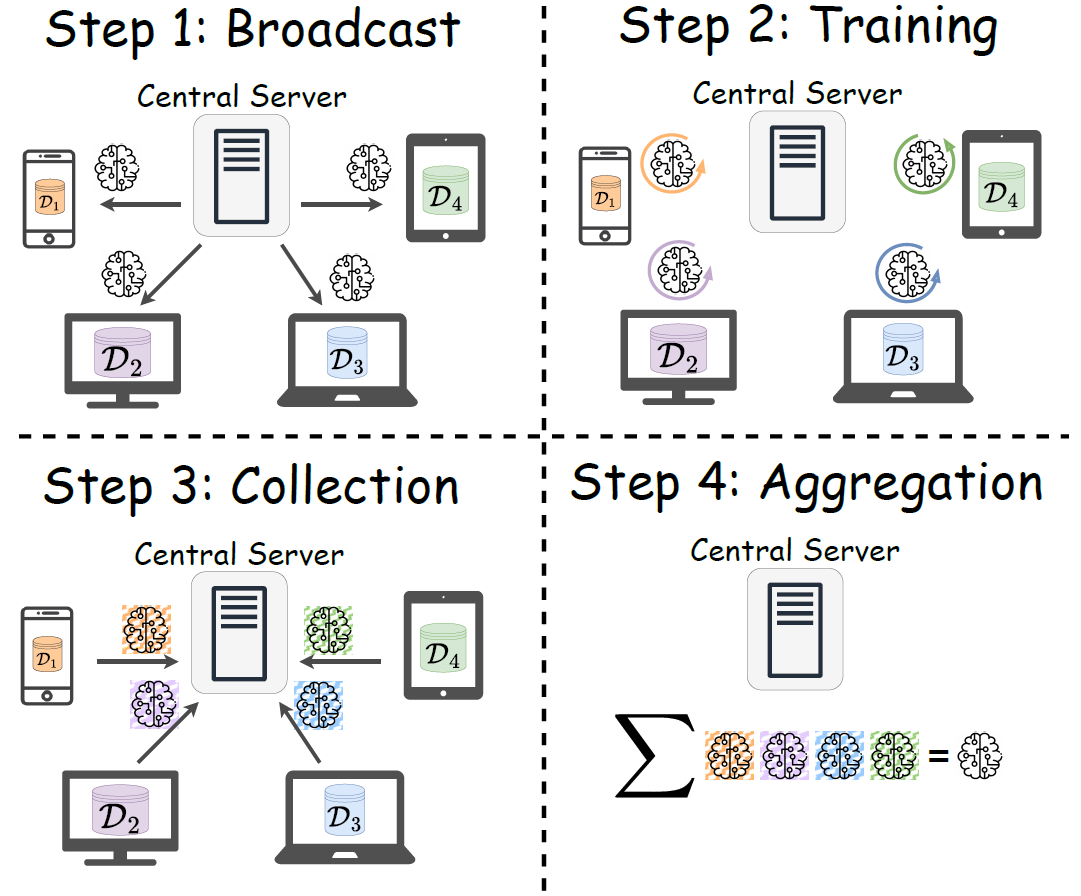
\includegraphics[width=0.60\textwidth]{figures/federated averaging.png}
    \caption{Chronological sequence of a Federated Learning communication round (broadcast, local client training, update collection, and server aggregation). Figure reproduced from Theologitis et al. \cite{theologitis2025fda}.}
    \label{fig:fl_overview}
\end{figure}

To solve this problem, the standard Federated Averaging (FedAvg) algorithm \cite{mcmahan2017communication} operates in communication rounds. At round $t$, the server selects a client cohort $S_t \subset K$ and broadcasts the global model $w_t$. The selected clients initialize their local models as $w_{t,0}^{(k)} = w_t$ and perform $\tau$ local steps of Stochastic Gradient Descent (SGD):
\begin{equation}
    w_{t, j+1}^{(k)} = w_{t,j}^{(k)} - \eta \nabla \ell(w_{t,j}^{(k)}; x)
    \label{eq:fedavg_sgd}
\end{equation}
After training, clients transmit their local updates $\Delta_{t}^{(k)} = w_{t,\tau}^{(k)} - w_t$ to the server, which aggregates them to compute the next global model:
\begin{equation}
    w_{t+1} = w_t + \frac{1}{|S_t|} \sum_{k \in S_t} \Delta_{t}^{(k)}
    \label{eq:fedavg_agg}
\end{equation}

\subsection{FedOpt: Server-Side Adaptive Optimization}
For modern large foundation models, transmitting full weight vectors $w \in \mathbb{R}^d$ introduces severe spatial communication overhead. Furthermore, client-level statistics are often noisy, and clients are typically stateless, preventing the direct use of adaptive optimizers on edge devices. To address this, the FedOpt framework \cite{reddi2021adaptive} shifts adaptive optimization to the server. Leveraging the adaptive optimization principles (e.g., Adam) discussed in Section \ref{sec:nn_sgd}, FedOpt allows the server to aggregate client parameter displacements $\Delta_t^{(k)} = w_{t,\tau}^{(k)} - w_t$ across the cohort $S_t$:
\begin{equation}
    \Delta_t = \frac{1}{|S_t|} \sum_{k \in S_t} \Delta_{t}^{(k)}
    \label{eq:fedopt_displacement}
\end{equation}
Because local updates move along descent trajectories, $\Delta_t$ represents the average parameter displacement. In gradient-based server optimizers (e.g., FedAdam, FedAdamW), this quantity defines an effective server pseudo-gradient with an inverted sign:
\begin{equation}
    \nabla_{\text{pseudo}, t} = - \Delta_t = - \frac{1}{|S_t|} \sum_{k \in S_t} \Delta_{t}^{(k)}
    \label{eq:fedopt_pseudo}
\end{equation}
ensuring that standard gradient-descent update steps ($w_{t+1} = w_t - \eta_s \nabla_{\text{pseudo}, t}$, as formalized in Chapter~\ref{chap:methodology}) step in the direction of cumulative local progress, or equivalently through an additive displacement step:
\begin{equation}
    w_{t+1} = \text{ServerOpt}(w_t, \Delta_t)
    \label{eq:fedopt_update}
\end{equation}

The motivation for server-side adaptive optimization in federated learning is distinct from its role in centralized training. In centralized settings, adaptive optimizers like Adam \cite{kingma2015adam} accelerate convergence by maintaining per-parameter learning rate scaling. In federated settings, the pseudo-gradient $\nabla_{\text{pseudo}, t}$ suffers from compounded noise: it is computed from a sampled client subset $S_t \subset K$ rather than all clients, and each client's local update reflects multiple SGD steps on heterogeneous data rather than a single gradient evaluation. Server-side momentum buffers smooth these noisy pseudo-gradients across rounds, providing a more stable optimization trajectory.

Furthermore, federated clients are inherently \emph{stateless}: they do not persist optimizer state (momentum, variance estimates) between communication rounds, as each round begins with a fresh initialization from the global model. This precludes the use of adaptive optimizers at the client level across rounds, making the server the only entity capable of maintaining long-term optimization history. Additionally, in parameter-efficient adaptation regimes (detailed in Section~\ref{sec:peft}), decoupled weight decay (AdamW \cite{loshchilov2019decoupled}) at the server provides implicit regularization on adapter parameters, helping prevent overfitting to the heterogeneous local distributions encountered during federated training.

While FedOpt stabilizes training and accelerates convergence, it still relies on rigid, static synchronization schedules (fixed $\tau$), ignoring local optimization dynamics and leading to temporal communication inefficiencies.

\subsection{Client Drift and Statistical Heterogeneity}
\label{sec:client_drift}
A defining challenge in federated learning is the statistical heterogeneity of client data distributions. In practice, client datasets $\mathcal{D}_k$ are rarely independent and identically distributed (IID). Instead, they exhibit various forms of heterogeneity: \emph{label skew}, where different clients possess data from different subsets of classes; \emph{quantity skew}, where the number of local training samples varies significantly across clients; and \emph{feature skew}, where the underlying input distributions differ even for the same label \cite{zhu2021federated}.

Under non-IID data, the local objective functions $F_k(w)$ may have significantly different minimizers. When clients perform multiple steps of local SGD on their heterogeneous data, their parameters drift toward distinct local optima that diverge from the global optimum. This phenomenon, known as \emph{client drift} \cite{karimireddy2020scaffold}, causes the aggregated global update to deviate from the true gradient direction, degrading convergence speed and final model quality.

The severity of client drift is formally analyzed by Li et al. \cite{li2020convergence}, who establish convergence bounds for FedAvg under non-IID data that depend on the degree of gradient dissimilarity across clients. Various drift-mitigation strategies have been proposed: FedProx \cite{li2020federated} adds a proximal regularization term to constrain local updates to remain close to the global model, while SCAFFOLD \cite{karimireddy2020scaffold} introduces variance reduction through control variates that correct for client drift at each local step. These methods highlight that \emph{monitoring and controlling the divergence between local and global model states is fundamental to stable federated optimization}, a principle that directly motivates the variance-driven synchronization approach explored later in this chapter.

\subsection{Dirichlet-Based Data Partitioning}
\label{sec:dirichlet}
To rigorously evaluate federated algorithms under controlled non-IID conditions, the research community has adopted the Dirichlet distribution as the standard tool for synthetic data partitioning \cite{hsu2019measuring, yurochkin2019bayesian, zhu2021federated}. For a classification task with $C$ classes and $K$ clients, each client $k$ receives a class proportion vector $p_k \sim \text{Dir}(\alpha)$, where $\text{Dir}(\alpha)$ denotes the symmetric Dirichlet distribution with concentration parameter $\alpha > 0$. Training samples of each class are then allocated to clients according to these sampled proportions.

The concentration parameter $\alpha$ provides a single scalar knob to control the degree of heterogeneity. As $\alpha \to 0$, the sampled proportion vectors become increasingly peaked, producing extreme label skew where individual clients may hold data from only a single class. Conversely, as $\alpha \to \infty$, the proportions converge to a uniform distribution, recovering the IID setting. Intermediate values (e.g., $\alpha = 0.5$ or $\alpha = 1.0$) produce moderate heterogeneity that reflects realistic scenarios where clients have partial but imbalanced class coverage. This configurability makes the Dirichlet partitioning scheme essential for conducting systematic ablation studies across varying degrees of statistical adversity.

\subsection{Communication Cost Quantification}
\label{sec:comm_cost}
To make the communication bottleneck concrete, consider the per-round transmission cost for foundation models. For a transformer backbone such as \texttt{roberta-base} ($125\,\text{M}$ parameters), transmitting the full model weights in standard 32-bit floating point precision requires approximately $500\,\text{MB}$ per client per synchronization round (or $\sim 250\,\text{MB}$ in 16-bit half-precision). Across a modest cohort of 10 clients over a 100-round federated training run, this results in up to $500\,\text{GB}$ of raw model transfers over uplink-constrained edge networks. In multi-billion parameter foundation architectures (such as Llama-2-7B with $\approx 7\times 10^9$ parameters), a single full-model synchronization demands approximately $28\,\text{GB}$ in FP32 per client per round, which is completely intractable in distributed federated settings.

To overcome this prohibitive uplink requirement, parameter-efficient fine-tuning (PEFT) methods restrict trainable parameters to compact modular adapters. In particular, Low-Rank Adaptation (LoRA, formalised in Section~\ref{sec:peft}) decomposes weight updates into low-rank factor matrices. When targeting the attention projection matrices of \texttt{roberta-base} with a compact adapter rank $r = 4$ (typically $r \in \{4, 8\}$), the communicated payload drops from $500\,\text{MB}$ to under $1\,\text{MB}$ per client per round, achieving a spatial compression ratio exceeding $500\times$. This substantial reduction demonstrates why low-rank parametrization is essential to make federated training of foundation models feasible across bandwidth-constrained edge networks.

\section{Parameter-Efficient Fine-Tuning}
\label{sec:peft}
The massive scale of foundation models renders traditional full fine-tuning (updating all $d$ parameters for a downstream task) increasingly impractical. Full fine-tuning requires storing not only the model weights but also the corresponding activation states, gradient tensors, and optimizer momentum buffers (e.g., first and second moment estimates for Adam) for every trainable parameter. For a model with $d$ parameters in mixed-precision training, the aggregate memory footprint can exceed $16d$ bytes, placing models with hundreds of millions or billions of parameters well beyond the capacity of commodity client hardware. Parameter-Efficient Fine-Tuning (PEFT) addresses this challenge by updating only a small subset of parameters while keeping the vast majority of pre-trained weights frozen.

\subsection{The PEFT Landscape}
\label{sec:peft_landscape}
Several families of PEFT techniques have been developed to balance parameter efficiency with representational capacity:
\begin{itemize}
    \item \textbf{Adapter Layers}: Introduced by Houlsby et al. \cite{houlsby2019parameter}, adapter modules inject small, learnable bottleneck layers between existing transformer feed-forward and self-attention projections. While parameter-efficient, they introduce structural changes that incur non-negligible inference latency.
    \item \textbf{Prefix Tuning}: Proposed by Li and Liang \cite{li2021prefix}, prefix tuning prepends learnable, continuous task-specific vectors directly to the key and value sequences of transformer attention layers, steering model behavior without modifying original parameters. However, prepending prefixes reduces the effective sequence length available for downstream context.
    \item \textbf{Prompt Tuning}: A further simplification of prefix tuning that prepends virtual token embeddings strictly to the input layer, offering high parameter economy but often exhibiting slower optimization convergence on complex tasks.
\end{itemize}

\subsection{Low-Rank Adaptation (LoRA)}
\label{sec:lora}
Among parameter-efficient adaptation paradigms, Low-Rank Adaptation (LoRA) \cite{hu2022lora} has emerged as the prevailing standard for both centralized and distributed environments. LoRA operates on the foundational hypothesis that weight updates during downstream task adaptation occupy a low intrinsic rank \cite{aghajanyan2021intrinsic}.

Rather than modifying a dense pre-trained weight matrix $W_0 \in \mathbb{R}^{d_{\text{out}} \times d_{\text{in}}}$ directly, LoRA parameterizes the weight update $\Delta W$ through a low-rank matrix decomposition:
\begin{equation}
    \Delta W = \frac{\alpha}{r} B A
    \label{eq:lora_factorization}
\end{equation}
where $A \in \mathbb{R}^{r \times d_{\text{in}}}$ denotes the down-projection matrix, $B \in \mathbb{R}^{d_{\text{out}} \times r}$ denotes the up-projection matrix, rank $r \ll \min(d_{\text{in}}, d_{\text{out}})$, and $\alpha$ is a constant scaling hyperparameter. The forward pass of a modified layer computes:
\begin{equation}
    h = W_0 x + \Delta W x = W_0 x + \frac{\alpha}{r} B A x
    \label{eq:lora_forward}
\end{equation}
Throughout fine-tuning, the pre-trained backbone weights $W_0$ remain completely frozen, receiving zero gradient updates. Only the compact factor matrices $A$ and $B$ are optimized. Under the canonical initialization scheme, $A$ is initialized with random Gaussian values $\mathcal{N}(0, \sigma^2)$, while $B$ is initialized to zero, ensuring that $\Delta W = \frac{\alpha}{r} B A = 0$ at training onset and the model's pre-trained predictions are exactly preserved prior to adaptation. The scaling factor $\frac{\alpha}{r}$ stabilizes the optimization dynamics when varying the adapter rank $r$, typically set such that $\alpha = 2r$. Figure~\ref{fig:lora_schematic} illustrates this architecture.

\begin{figure}[htbp]
    \centering
    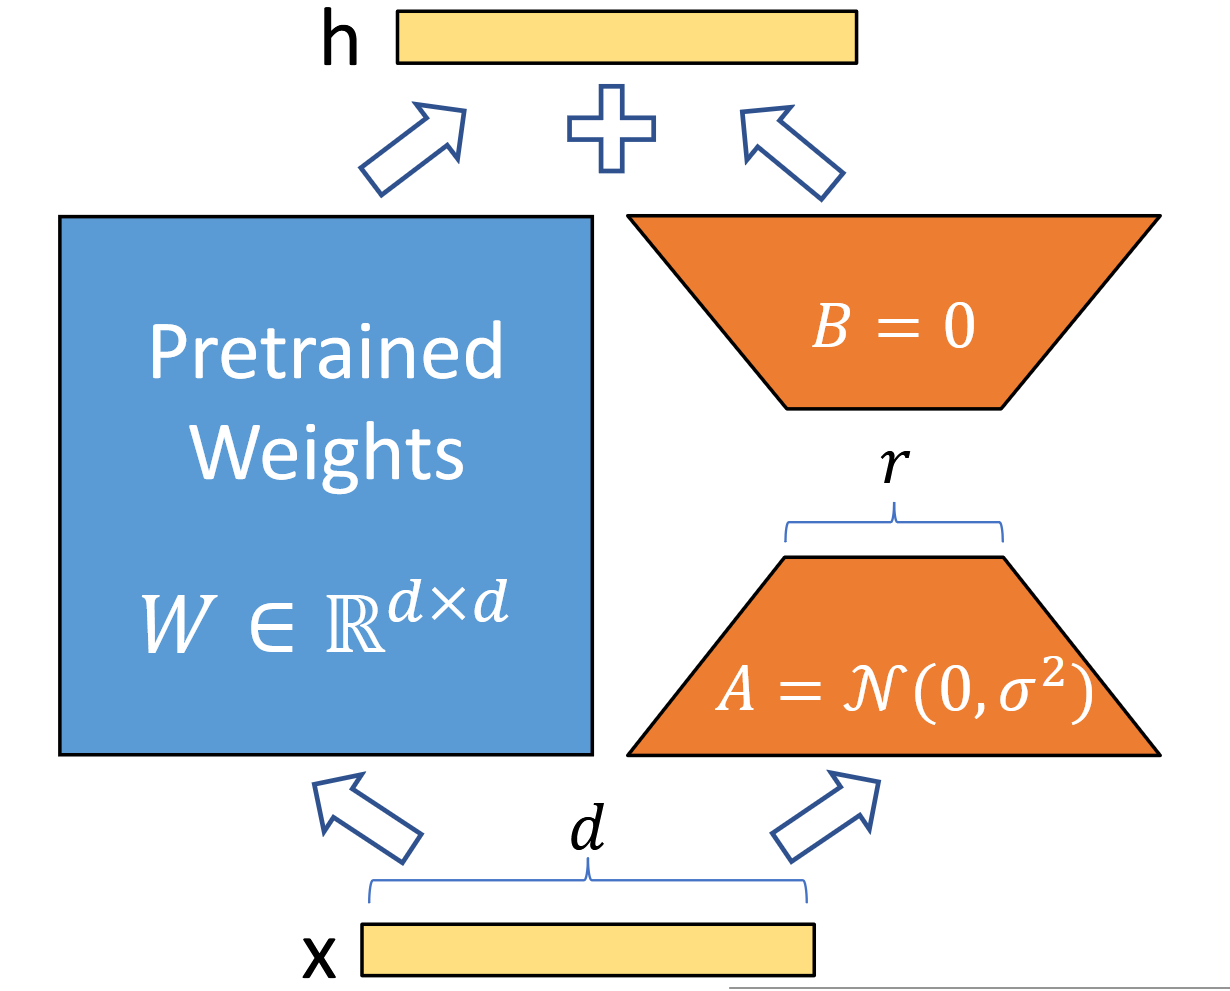
\includegraphics[width=0.4\textwidth]{figures/lora_figure.png}
    \caption{Low-Rank Adaptation (LoRA) schematic: decomposition of weight updates into low-rank matrices $A$ and $B$ alongside frozen pretrained weights $W$. Figure reproduced from Hu et al. \cite{hu2022lora}.}
    \label{fig:lora_schematic}
\end{figure} 

Unlike adapter layers, LoRA introduces zero additional inference latency: upon completion of training, the factorized update $\frac{\alpha}{r} BA$ can be folded directly into the pre-trained weights ($W_{\text{final}} = W_0 + \frac{\alpha}{r} BA$) via simple matrix addition. In centralized settings, extensions such as QLoRA \cite{dettmers2023qlora} (which integrates 4-bit NormalFloat base quantization) and AdaLoRA \cite{zhang2023adalora} (which dynamically allocates rank budgets across layers) have further highlighted the versatility of the low-rank paradigm.

\subsection{Structural and Dynamic Asymmetry in LoRA Matrices}
\label{sec:lora_asymmetry}
An essential, frequently overlooked property of the LoRA decomposition is the inherent asymmetry between its two factor matrices. Functionally, the down-projection matrix $A \in \mathbb{R}^{r \times d_{\text{in}}}$ compresses input features from high-dimensional representations into the low-rank bottleneck, whereas the up-projection matrix $B \in \mathbb{R}^{d_{\text{out}} \times r}$ expands compressed representations back to the original dimensionality. These distinct projection roles produce asymmetric gradient dynamics during backpropagation.

Furthermore, the canonical initialization scheme creates an acute temporal asymmetry: because $B = 0$ at initialization, the initial gradients with respect to $A$ ($\nabla_A \mathcal{L} \propto B^\top \nabla_h \mathcal{L}$) are initially zero, whereas the gradients with respect to $B$ ($\nabla_B \mathcal{L} \propto \nabla_h \mathcal{L} (A x)^\top$) immediately receive non-zero projections from the Gaussian-initialized $A$. Consequently, the optimization trajectories, convergence velocities, and parameter variance profiles of $A$ and $B$ diverge substantially during early training rounds, with matrix $B$ typically manifesting significantly higher drift. In federated learning, this asymmetry implies that treating both coordinate matrices identically during aggregation or synchronization scheduling is fundamentally suboptimal.

\section{Federated Low-Rank Adaptation}
\label{sec:fedlora}
Having established standard LoRA and the core FL framework, combining the two paradigms, formalized as Federated Low-Rank Adaptation (FedLoRA) \cite{yang2025federated}, is a natural evolution to reduce the massive communication costs of federated learning. In a typical FL setting, transmitting full model updates $w \in \mathbb{R}^d$ imposes severe network strain. By adopting LoRA, clients only train and transmit the low-rank matrices $A$ and $B$, which drastically reduces the spatial communication overhead of federated synchronization.

A comprehensive survey of FedLoRA \cite{yang2025federated} categorizes the primary challenges in this domain into distributed learning stability, data heterogeneity, and efficiency. To address these challenges, several frameworks have been proposed. For instance, FedIT \cite{zhang2023towards} applies standard federated averaging directly to LoRA parameters. To mitigate communication costs further and ensure exact updates, FFA-LoRA \cite{sun2024improving} freezes the down-projection matrices $A$ across all clients, allowing clients to update and transmit only the up-projection matrices $B$. Other approaches, such as FLoRA \cite{wang2024flora}, support heterogeneous-rank adapters among clients to accommodate varying device capacities.

Despite its benefits, aggregating independent low-rank matrices from clients introduces a critical issue known as \emph{LoRA Aggregation Discordance} \cite{yang2025federated}. When standard federated averaging (FedAvg) is applied separately to the client-specific matrices $A_i$ and $B_i$, it introduces a fundamental mathematical inconsistency:
\begin{equation}
    \frac{1}{N} \sum_{i=1}^{N} (B_i A_i) \neq \left( \frac{1}{N} \sum_{i=1}^{N} B_i \right) \left( \frac{1}{N} \sum_{i=1}^{N} A_i \right)
    \label{eq:lora_inconsistency}
\end{equation}
This inequality demonstrates that independent averaging of $B_i$ and $A_i$ fails to reconstruct the true average of the weight updates due to the non-linear, bilinear nature of matrix multiplication. As a result, applying FedAvg directly to these factorized matrices leads to inaccurate global aggregation and severe model degradation. 

To address this discordance, the literature proposes several alternative strategies \cite{yang2025federated}. One approach is full-size matrix aggregation, where clients reconstruct the full $\Delta W = \frac{\alpha}{r} BA$ before transmission; however, this entirely negates the spatial communication benefits of LoRA. Another approach involves SVD recalculation, where the server aggregates full matrices and then performs Singular Value Decomposition to extract new low-rank factors, which introduces prohibitive computational overhead at the server. Compared to these computationally or communication-heavy alternatives, alternating single-matrix aggregation has emerged as a highly efficient and structurally sound solution.

\section{Robust Low-Rank Adaptation}
\label{sec:rolora}
While LoRA successfully reduces the spatial communication cost, the aggregation inconsistency described above poses a fundamental barrier to its deployment in federated settings. RoLoRA addresses this without sacrificing adapter expressiveness.

To resolve this inconsistency without limiting adapter expressiveness, RoLoRA \cite{chen2025robust} introduces an alternating optimization and aggregation framework. Instead of permanently freezing one of the low-rank matrices, RoLoRA alternates the active training coordinate space across communication rounds.

\begin{figure}[htbp]
    \centering
    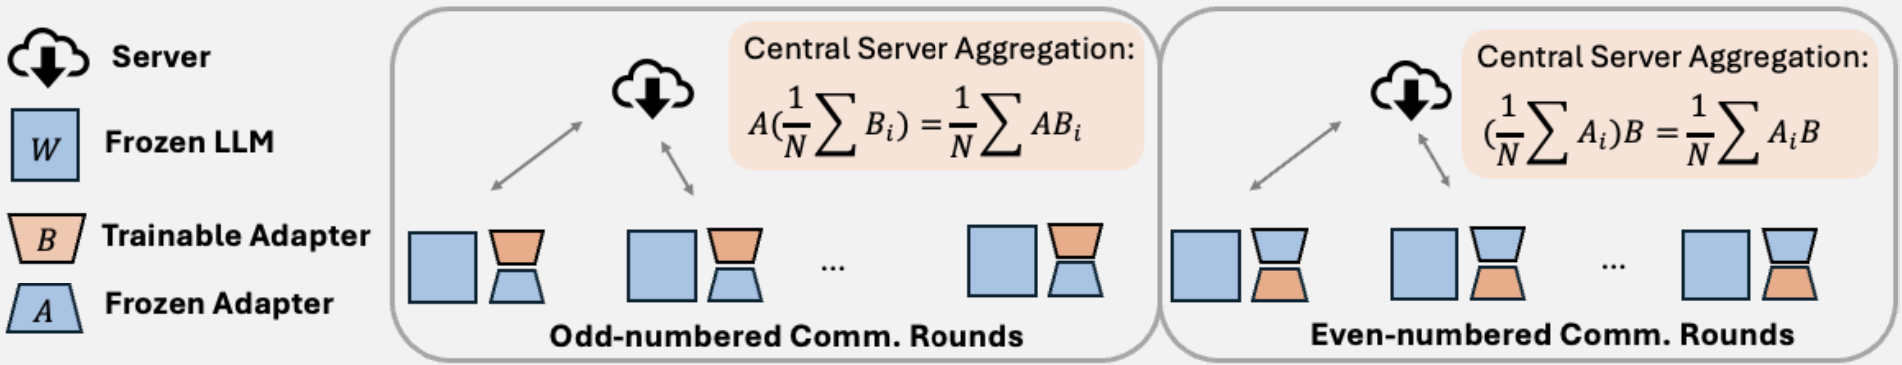
\includegraphics[width=0.75\textwidth]{figures/rolora_framework.png}
    \caption[Robust Low-Rank Adaptation (RoLoRA) alternating optimization scheme.]{Robust Low-Rank Adaptation (RoLoRA) alternating optimization scheme. In each round, one low-rank matrix is frozen globally while the other is trained and aggregated linearly. \emph{Note: The schematic reproduced from Chen et al.~\cite{chen2025robust} uses row-vector notation ($AB$); under our standard column-vector convention ($BA$), odd rounds aggregate $(\frac{1}{N}\sum B_i)A$ and even rounds aggregate $B(\frac{1}{N}\sum A_i)$.}}
    \label{fig:rolora_framework}
\end{figure}

\noindent \emph{Note on notation:} While Chen et al. \cite{chen2025robust} designate their low-rank product as $AB$ by naming the up-projection $A$ and down-projection $B$, we maintain the standard LoRA convention $\Delta W = \frac{\alpha}{r} BA$ \cite{hu2022lora} throughout this thesis to preserve mathematical consistency with common PEFT architectures and the formal framework developed in Chapter~\ref{chap:methodology}.

In odd-numbered communication rounds ($2t+1$), the down-projection matrix $A^t$ is globally frozen and shared across all clients $i$, while only the up-projection matrix $B$ is trained locally. The server then aggregates these updates:
\begin{equation}
    B^{t+1} = \frac{1}{N} \sum_{i=1}^{N} B^{t+1}_i
    \label{eq:rolora_B_agg}
\end{equation}
Because $A^t$ is identical across all clients, the aggregation is strictly linear, introducing no spatial interference:
\begin{equation}
    \frac{1}{N} \sum_{i=1}^{N} (B^{t+1}_i A^t) = \left( \frac{1}{N} \sum_{i=1}^{N} B^{t+1}_i \right) A^t = B^{t+1} A^t
    \label{eq:rolora_B_proof}
\end{equation}

In even-numbered communication rounds ($2t+2$), the aggregated up-projection matrix $B^{t+1}$ is frozen, while the clients update the down-projection matrix $A$ locally. The server aggregates these updates:
\begin{equation}
    A^{t+1} = \frac{1}{N} \sum_{i=1}^{N} A^{t+1}_i
    \label{eq:rolora_A_agg}
\end{equation}
Since $B^{t+1}$ is now identical across all clients, linearity is preserved:
\begin{equation}
    \frac{1}{N} \sum_{i=1}^{N} (B^{t+1} A^{t+1}_i) = B^{t+1} \left( \frac{1}{N} \sum_{i=1}^{N} A^{t+1}_i \right) = B^{t+1} A^{t+1}
    \label{eq:rolora_A_proof}
\end{equation}
This alternating optimization enables full parameter space exploration while maintaining zero-interference linear aggregations throughout the federated training process.

\section{Federated Dynamic Averaging}
\label{sec:fda}
Having resolved the spatial communication bottleneck through RoLoRA's linearized aggregation, we now address the temporal dimension: controlling the synchronization frequency based on actual training dynamics rather than a fixed schedule.

Federated Dynamic Averaging (FDA) and its optimization variant FDA-Opt \cite{theologitis2025fda} were developed to optimize the training schedule dynamically. FDA is rooted in the principles of Geometric Monitoring \cite{sharfman2006geometric}, a framework originally developed for threshold function monitoring over distributed data streams.

\subsection{Geometric Monitoring Foundations}
The core insight of geometric monitoring is that a global condition over distributed data can be decomposed into local conditions that each node monitors independently. Consider $N$ distributed nodes, each holding a local state vector $v_i(t)$ that evolves over time. The global state is the average $\bar{v}(t) = \frac{1}{N}\sum_{i=1}^{N} v_i(t)$. The monitoring objective is to detect when a threshold function $f(\bar{v}(t))$ crosses a predefined boundary, without requiring continuous global synchronization.

Geometric monitoring achieves this through the concept of \emph{safe zones}. Each node $i$ defines a bounding region around a reference point $e_i$ (typically the last synchronized global estimate). As long as the local drift vector $\delta_i(t) = v_i(t) - e_i$ remains within its safe zone, the global condition is guaranteed to hold by a convexity argument: if all local states lie within a convex safe zone centered around the global reference, their average must also lie within that zone. Crucially, this means that \emph{no communication is necessary} as long as every node's local constraint is satisfied. A synchronization round is triggered only when at least one node's drift exits its safe zone, indicating that the global condition may have been violated.

FDA adapts this distributed monitoring framework to the federated learning setting. The ``state vectors'' become local model parameter updates, the ``threshold function'' becomes model variance (measuring client drift divergence), and the ``safe zone'' is defined by a variance budget $\theta$. When local parameter drift across clients causes the variance to exceed $\theta$, synchronization is triggered. This reformulation transforms the rigid, schedule-based synchronization of standard FL into an event-driven protocol that communicates only when training dynamics demand it.

For a sampled subset of clients $S_t$ at communication round $t$, let $\Delta_{t,i}^{(k)} = w_{t,i}^{(k)} - w_{t,0}$ denote the local update of client $k$ at step $i$ relative to the initial global model $w_{t,0}$. The average update (pseudo-gradient) across all clients is defined as:
\begin{equation}
    g_{t,i} = \frac{1}{|S_t|} \sum_{k \in S_t} \Delta_{t,i}^{(k)}
    \label{eq:fda_pseudo}
\end{equation}
The model variance quantifies the dispersion of local client updates in the parameter space and is defined as:
\begin{equation}
    \text{Var}(W_{t,i}) = \frac{1}{|S_t|} \sum_{k \in S_t} \left\| \Delta_{t,i}^{(k)} \right\|_2^2 - \left\| g_{t,i} \right\|_2^2
    \label{eq:fda_variance}
\end{equation}
Here, the first term measures the average local training progress across clients, while the second term captures the magnitude of the aggregated global step. Consequently, a low model variance value signifies either negligible local gradient progress or, more favorably, highly aligned local updates across participating clients where local optimization trajectories coincide. Conversely, a high variance reading manifests when clients achieve substantial local parameter movement along divergent optimization vectors towards conflicting local minima, signaling the onset of severe client drift.


During local training, clients track model variance. Computing this exact variance requires full-dimensional vector operations, which can be computationally expensive and communication-heavy to track continuously in a distributed setting. To address this, the original FDA protocol utilizes the Alon-Matias-Szegedy (AMS) sketch \cite{alon1996space}, a randomized algorithm that efficiently approximates the $L_2$ norm (and thus the variance) using minimal memory and sub-linear space. While full-parameter models require randomized sketching to approximate variance in sub-linear memory, we show in Chapter~\ref{chap:methodology} that restricting geometric monitoring to compact low-rank coordinate tensors allows exact variance evaluation with negligible computational and memory overhead, rendering probabilistic sketching unnecessary in federated LoRA regimes.

Synchronization is triggered immediately if the variance exceeds a dynamic threshold: $\text{Var}(W_{t,i}) > \theta_t$. Because the variance magnitude evolves by orders of magnitude from early to late training stages, FDA-Opt dynamically scales this threshold across rounds using a linear prediction based on the previous round's termination step $s_t$:
\begin{equation}
    \theta_{t+1} = \text{var}_t \cdot \frac{\tau}{2 s_t}
    \label{eq:fda_threshold}
\end{equation}
where $\text{var}_t$ is the actual variance at termination in round $t$, $s_t$ is the termination step, and $\tau$ is the target training duration. This linear threshold prediction assumes that standard training variance typically grows linearly and monotonically during a round. Furthermore, to eliminate the synchronization overhead of checking variance at every training step, queries are restricted to a sparse subset of steps (typically once per epoch), mitigating the communication bottleneck of distributed geometric checks.

While RoLoRA resolves the spatial aggregation inconsistency and FDA addresses the temporal communication cadence, combining the two paradigms requires careful algorithmic formulation. In particular, low-rank parameter trajectories exhibit heightened variance volatility, and alternating optimization demands decoupled threshold management. To address these challenges, Chapter~\ref{chap:methodology} formalizes \textbf{FDA-RoLoRA} to combine dynamic averaging with alternating low-rank adaptation, explaining how it internally deploys a dual-track threshold mechanism to track subspace divergence independently. The concrete execution loops of both baseline protocols are formally summarized in Section~\ref{sec:foundational_protocols} before introducing our synthesized methodology.

\chapter{Methodology}
\label{chap:methodology}

The research presented in this thesis investigates the integration of Federated Dynamic Averaging (FDA) \cite{theologitis2025fda} with Parameter-Efficient Low-Rank Adaptation (LoRA) \cite{hu2022lora}. By bridging dynamic variance-driven synchronization with low-rank parameter factorizations, this work aims to jointly optimize the spatial and temporal dimensions of federated learning.

\section{Combining Dynamic Averaging with Federated LoRA}
\label{sec:fda_lora_taxonomy}
Existing literature in Parameter-Efficient Federated Fine-Tuning focuses almost exclusively on spatial parameter compression, while universally relying on static Federated Averaging (FedAvg) \cite{mcmahan2017communication} for temporal synchronization. Under standard FedAvg, all clients execute a predetermined, fixed number of local epochs ($\tau = E$) regardless of local optimization drift, data heterogeneity, or gradient volatility.

The concept of integrating dynamic averaging into federated low-rank architectures envisions replacing rigid, static FedAvg schedules with adaptive, variance-driven averaging. Crucially, combining FDA with different federated LoRA variants cannot be treated as a single, one-size-fits-all formula. Because distinct PEFT methods manipulate low-rank matrices through fundamentally different mechanisms—ranging from simultaneous factor updates to frozen projections, sparse allocations, or alternating coordinates—each pairing suggests a distinct architectural design:

\begin{itemize}
    \item \textbf{FDA + FedLoRA}: Explores dynamic synchronization alongside standard simultaneous training of low-rank matrices $A$ and $B$. In this configuration, dynamic averaging could monitor the joint parametric drift or product-space variance of the complete adapter. While this pairing retains the characteristic bilinear aggregation of standard FedLoRA ($\frac{1}{N}\sum A_i B_i \neq (\frac{1}{N}\sum A_i)(\frac{1}{N}\sum B_i)$), it represents the most direct, unconstrained synthesis of dynamic scheduling and low-rank adaptation.
    \item \textbf{FDA + FFA-LoRA}: Explores dynamic averaging under frozen down-projections \cite{sun2024improving}, where matrix $A$ remains fixed after random initialization. Because parameter evolution is restricted solely to the up-projection $B$, dynamic variance monitoring simplifies to tracking a single active subspace coordinate space.
    \item \textbf{FDA + SLoRA}: Explores dynamic synchronization tailored to sparse low-rank parameter representations \cite{babakniya2023slora}, where threshold adaptation and variance estimation could be structured around coordinate-sparse adapter allocations across clients.
    \item \textbf{FDA + RoLoRA (Our investigation)}: Explores dynamic averaging in conjunction with alternating coordinate optimization \cite{chen2025robust}. By alternating active updates between down-projection matrix $A$ and up-projection matrix $B$ across global communication rounds, this avenue naturally isolates each subspace, preserving update linearity ($\frac{1}{N}\sum A B_i = A(\frac{1}{N}\sum B_i)$) and enabling independent, decoupled threshold tracking ($\theta_A, \theta_B$).
\end{itemize}

Among these architectural possibilities, we select \textbf{FDA + RoLoRA} as our focal investigation due to the unique mathematical advantages of coordinate alternation. By isolating updates to a single low-rank factor per communication round, RoLoRA provides strict linearity in parameter aggregation, eliminating inter-factor interference. This structural property provides an exceptionally clean theoretical foundation for formulating decoupled subspace variance tracking with independent geometric thresholds. We consider the broader taxonomy—such as joint variance tracking in simultaneous FedLoRA or coordinate-sparse thresholding in SLoRA—as promising avenues for future research.

The key insight enabling this integration is that FDA's variance monitoring can be applied independently to each subspace, as RoLoRA's alternating scheme naturally isolates the optimization trajectories of the down-projection ($A$) and up-projection ($B$) matrices. To regulate threshold updates across communication rounds, the framework adopts a responsive, parameter-free midpoint-scaling threshold update rule that dynamically adapts synchronization intervals to local client drift.

\section{Foundational Precursor Protocols: RoLoRA and FDA}
\label{sec:foundational_protocols}

To rigorously contextualize the design of FDA-RoLoRA, we examine the operational execution loops of its two constituent foundational frameworks: Federated Dynamic Averaging (FDA) \cite{theologitis2025fda} and Robust Low-Rank Adaptation (RoLoRA) \cite{chen2025robust}. While both methods address fundamental inefficiencies in decentralized learning, they tackle orthogonal dimensions of the federated optimization bottleneck:

\begin{itemize}
    \item \textbf{FDA (Temporal Optimization, Full-Rank Model Space)}: Evaluates the dispersion of local client updates in parameter space. By deploying geometric safe zones via the AMS sketch, FDA replaces static round schedules with variance-triggered synchronization, dynamically terminating local training at $e^* \le E$ when client drift exceeds a scalar threshold $\theta$. However, the standard protocol assumes simultaneous parameter updates over the full model weight space, leaving low-rank factorized architectures unaddressed.
    \item \textbf{RoLoRA (Spatial Optimization, Fixed Local Schedule)}: Eliminates bilinear aggregation inconsistency by alternating coordinate optimization between low-rank factor matrices ($A$ and $B$) across global communication rounds. When factor $B$ is trained, down-projection $A$ is frozen, preserving update linearity ($\frac{1}{N}\sum A_i B = (\frac{1}{N}\sum A_i)B$). However, RoLoRA enforces a rigid, fixed local epoch schedule ($E$) across all clients and rounds, leaving temporal synchronization unoptimized.
\end{itemize}

Algorithm~\ref{alg:std_fda} and Algorithm~\ref{alg:std_rolora} summarize the algorithmic structures of FDA and RoLoRA side-by-side.

\vspace{0.2cm}
\noindent
\begin{minipage}[t]{0.485\textwidth}
\begin{algorithm}[H]
\SetAlFnt{\footnotesize}
\SetAlCapFnt{\small}
\SetAlCapNameFnt{\small}
\caption{FDA}
\label{alg:std_fda}
\KwIn{Clients $K$, cohort $|S_r|$, initial $\theta_0$, limit $E$}
Initialize global parameters $W_0$\;
\For{round $r = 0, 1, 2, \dots$}{
    Broadcast $W_0^{(r)}$ to cohort $S_r$\;
    \For{epoch $e = 1$ \KwTo $E$}{
        \ForEach{client $i \in S_r$ \textbf{in parallel}}{
            $W_{i,e}^{(r)} \leftarrow W_{i,e-1}^{(r)} - \eta_c \nabla \mathcal{L}_i$\;
            $\Delta_i^{(e)} = W_{i,e}^{(r)} - W_0^{(r)}$\;
        }
        Evaluate AMS variance\;
        \If{$\text{Var}(\Delta^{(e)}) > \theta_r$}{
            $e^* \leftarrow e$; \textbf{break}\;
        }
    }
    $W_0^{(r+1)} \leftarrow \frac{1}{|S_r|} \sum_{i \in S_r} W_{i,e^*}^{(r)}$\;
    Update scalar threshold $\theta_{r+1}$\;
}
\end{algorithm}
\end{minipage}\hfill
\begin{minipage}[t]{0.485\textwidth}
\begin{algorithm}[H]
\SetAlFnt{\footnotesize}
\SetAlCapFnt{\small}
\SetAlCapNameFnt{\small}
\caption{RoLoRA}
\label{alg:std_rolora}
\KwIn{Clients $K$, cohort $|S_r|$, fixed epoch limit $E$}
Initialize $W = W_{pretrained} + A_0 B_0$\;
\For{round $r = 0, 1, 2, \dots$}{
    Select active $\mathcal{M}^{(r)} \in \{B, A\}$\;
    Freeze complementary matrix\;
    Broadcast active $W_{act}^{(r)}$ to $S_r$\;
    \For{epoch $e = 1$ \KwTo $E$}{
        \ForEach{client $i \in S_r$ \textbf{in parallel}}{
            Train $\mathcal{M}^{(r)}$ on local data\;
            $\Delta_i = W_{i,e}^{(r)} - W_{act}^{(r)}$\;
        }
    }
    Collect client drifts $\{\Delta_i\}_{i \in S_r}$\;
    $\Delta_{agg} \leftarrow \frac{1}{|S_r|} \sum_{i \in S_r} \Delta_i$\;
    $W_{act}^{(r+1)} \leftarrow W_{act}^{(r)} + \Delta_{agg}$\;
}
\end{algorithm}
\end{minipage}
\vspace{0.3cm}

Contrasting these two protocols reveals the central architectural gap: RoLoRA provides the necessary update linearity to eliminate spatial distortion, but lacks adaptive temporal control; FDA provides dynamic temporal adaptivity, but cannot handle coordinate-isolated, asymmetric low-rank subspaces with a single scalar threshold. This limitation directly motivates our proposed \textbf{FDA-RoLoRA}, which synthesizes alternating coordinate isolation with decoupled subspace variance tracking via an internal dual-track threshold mechanism.

\clearpage
\section{Notation and Hyperparameters}
Consider a global communication round indexed by $r$, during which an active matrix $\mathcal{M}^{(r)} \in \{A, B\}$ is designated for client-side optimization. Within round $r$, local client optimization progresses through discrete local epoch iterations $e \in \mathbb{N}$, culminating in a final realized local epoch count $e^* \in \mathbb{N}$ at the instant synchronization is triggered. At any given evaluation epoch $e$, each client $i$ computes its raw subspace parametric drift $\Delta_i^{(e)}$ relative to the starting global parameters. Rather than projecting these parameter updates back to the expanded model weight space, the framework evaluates the direct subspace variance $\text{Var}_{subspace}(\Delta^{(e)})$ exclusively on the low-rank coordinate tensors of the active matrix.

The operational boundaries and adaptive behavior of FDA-RoLoRA are governed by a set of global hyperparameters. Local client training is bounded between a minimum epoch floor $e_{min} \in \mathbb{N}$ and a maximum epoch ceiling $e_{max} \in \mathbb{N}$. To accommodate the distinct drift dynamics of alternating low-rank factor matrices, FDA-RoLoRA internally implements a dual-track threshold mechanism: synchronization timing is controlled by two persistent, decoupled variance thresholds $\theta_A, \theta_B \in \mathbb{R}^+$, from which the active threshold $\theta_{current}^{(r)}$ is dynamically mapped to match $\mathcal{M}^{(r)}$. Threshold adaptation across rounds is governed by the direct midpoint-scaling update. A comprehensive summary of mathematical symbols, tensor shapes, and hyperparameters is provided in Table~\ref{tab:methodology_notation}.

\begin{table}[htbp]
\centering
\small
\caption{Summary of mathematical notation and system hyperparameters.}
\label{tab:methodology_notation}
\resizebox{\textwidth}{!}{
\begin{tabular}{lll}
\toprule
\textbf{Symbol} & \textbf{Domain / Dimensions} & \textbf{Description} \\
\midrule
$W_{pretrained}$ & $\mathbb{R}^{d_{out} \times d_{in}}$ & Frozen backbone model parameter weights \\
$r_{rank}$ & $\mathbb{N}$ ($r_{rank} \ll \min(d_{in}, d_{out})$) & Intrinsic low-rank adapter rank dimension \\
$A$ & $\mathbb{R}^{r_{rank} \times d_{in}}$ & Low-rank down-projection factor matrix \\
$B$ & $\mathbb{R}^{d_{out} \times r_{rank}}$ & Low-rank up-projection factor matrix \\
$K$ & $\mathbb{N}^+$ & Total number of decentralized client nodes in the federation \\
$S_r$ & $S_r \subseteq \{1, \dots, K\}$ & Sampled cohort of participating clients in round $r$ \\
$r$ & $\mathbb{N}_0 = \{0, 1, 2, \dots\}$ & Global communication round index \\
$\mathcal{M}^{(r)}$ & $\{B, A\}$ & Designated active parameter matrix in round $r$ \\
$W_{act}^{(r)}$ & Active matrix tensor & Global parameters of the active matrix broadcast to cohort $S_r$ \\
$e$ & $\{1, \dots, e_{max}\}$ & Local training epoch index within a round \\
$e_{min}, e_{max}$ & $\mathbb{N}^+$ ($e_{min} \le e_{max}$) & Minimum epoch floor and maximum epoch ceiling \\
$e^*$ & $[e_{min}, e_{max}]$ & Realized local epoch count at synchronization trigger \\
$\Delta_i^{(e)}$ & Matching $\mathcal{M}^{(r)}$ & Subspace parametric drift of client $i$ at epoch $e$ \\
$\text{Var}_{subspace}$ & $\mathbb{R}_{\ge 0}$ & Subspace drift variance across cohort $S_r$ (Eq.~\ref{eq:subspace_var}) \\
$\theta_A, \theta_B$ & $\mathbb{R}^+$ & Persistent, decoupled variance thresholds for tracks $A$ and $B$ \\
$\theta_{current}^{(r)}$ & $\mathbb{R}^+$ & Active threshold loaded for round $r$ ($\theta_A$ or $\theta_B$) \\
$\theta_{target}^{(r)}$ & $\mathbb{R}^+$ & Target threshold proposal computed via midpoint scaling \\
$\nabla_{pseudo}^{(r)}$ & Matching $\mathcal{M}^{(r)}$ & Aggregated server-side pseudo-gradient (Eq.~\ref{eq:pseudo_grad}) \\
$\eta_c, \eta_s$ & $\mathbb{R}^+$ & Local client learning rate and global server learning rate \\
\bottomrule
\end{tabular}
}
\end{table}


\clearpage
\begin{algorithm}[H]
\caption{FDA-RoLoRA}
\label{alg:fda_rolora}
\KwIn{Clients $K$, cohort size $|S_r|$, server learning rate $\eta_s$, local learning rate $\eta_c$, min/max epochs $e_{min}, e_{max}$, initial thresholds $\theta_A, \theta_B$}
Initialize global parameters $W = W_{pretrained} + A_0 B_0$\;
Initialize persistent thresholds $\theta_A, \theta_B$ and decoupled server optimizer states (for matrices $A$ and $B$)\;
Set first-round calibration flags: $\text{FirstRound}_A \leftarrow \text{True}, \text{FirstRound}_B \leftarrow \text{True}$\;
\For{round $r = 0, 1, 2, \dots$}{
    Determine active matrix $\mathcal{M}^{(r)} \in \{B, A\}$ (alternate $B$-first each round)\;
    Load active threshold $\theta_{current}^{(r)} \leftarrow \theta_{\mathcal{M}^{(r)}}$ and active server optimizer\;
    Sample client cohort $S_r \subseteq \{1, \dots, K\}$\;
    Server broadcasts active parameters $W_{act}^{(r)}$ to sampled cohort $S_r$\;
    
    \For{local epoch $e = 1$ \KwTo $e_{max}$}{
        \ForEach{client $i \in S_r$ \textbf{in parallel}}{
            Train locally for one epoch on private data: $W_{i,e}^{(r)} \leftarrow W_{i,e-1}^{(r)} - \eta_c \nabla \mathcal{L}_i(W_{i,e-1}^{(r)})$\;
            Compute subspace drift: $\Delta_i^{(e)} = W_{i,e}^{(r)} - W_{act}^{(r)}$\;
        }
        \If{$e \ge e_{min}$}{
            Server collects drifts $\{\Delta_i^{(e)}\}_{i \in S_r}$ and evaluates cohort variance $\text{Var}_{subspace}(\Delta^{(e)})$ via Eq.~\ref{eq:subspace_var}\;
            \If{$\text{FirstRound}_{\mathcal{M}^{(r)}}$}{
                $e^* \leftarrow e$\;
                $\text{FirstRound}_{\mathcal{M}^{(r)}} \leftarrow \text{False}$\;
                \textbf{break}\;
            }
            \If{$\text{Var}_{subspace}(\Delta^{(e)}) > \theta_{current}^{(r)}$ \textbf{or} $e = e_{max}$}{
                $e^* \leftarrow e$\;
                \textbf{break}\;
            }
        }
    }
    
    Server computes pseudo-gradient $\nabla_{pseudo}^{(r)} = - \frac{1}{|S_r|} \sum_{i \in S_r} \Delta_i^{(e^*)}$ via Eq.~\ref{eq:pseudo_grad}\;
    Update active matrix threshold $\theta_{\mathcal{M}^{(r)}} \leftarrow \theta_{target}^{(r)}$ via midpoint scaling (Eq.~\ref{eq:std_update}), keeping inactive threshold frozen\;
    Apply active server optimizer (Gradient Descent / FedAvg with $\eta_s$) to update $W_{act}^{(r+1)}$ via Eq.~\ref{eq:server_sgd}\;
}
\end{algorithm}
\clearpage

\section{FDA-RoLoRA Initialization and Subspace Toggling}
At the start of round $r$, the server determines the active target matrix $\mathcal{M}^{(r)} \in \{B, A\}$ adhering to a $B$-first alternating schedule. Internally, FDA-RoLoRA operates a dual-track threshold mechanism that maintains independent variance tracking for each coordinate space. To govern the local synchronization dynamics, the system loads the persistent threshold corresponding exclusively to the active matrix:
\begin{equation}
    \theta_{current}^{(r)} = \begin{cases} 
    \theta_A & \text{if } \mathcal{M}^{(r)} = A \\ 
    \theta_B & \text{if } \mathcal{M}^{(r)} = B 
    \end{cases}
    \label{eq:active_threshold}
\end{equation}
The active weight matrix is initialized across all sampled clients $i \in S_r$ using the global model parameters broadcast by the server:
\begin{equation}
    W_{i,0}^{(r)} = W_{act}^{(r)}
    \label{eq:client_init}
\end{equation}

\section{Local Training and Direct Subspace Variance}
Clients advance local parameters using independent Stochastic Gradient Descent \cite{robbins1951stochastic} steps. For client $i$ at local step $t$, the parameter update operates on the active parameter tensor:
\begin{equation}
    W_{i,t}^{(r)} = W_{i,t-1}^{(r)} - \eta_c \nabla \mathcal{L}_i(W_{i,t-1}^{(r)})
    \label{eq:local_sgd}
\end{equation}
where $\eta_c$ is the local learning rate and $\mathcal{L}_i$ is the client's empirical loss.

Local training proceeds epoch-by-epoch. At each epoch boundary $e \ge e_{min}$, participating clients compute their raw subspace parametric drift relative to the starting global parameter state:
\begin{equation}
    \Delta_i^{(e)} = W_{i,e}^{(r)} - W_{act}^{(r)}
    \label{eq:drift}
\end{equation}
To minimize communication overhead, exact variance is computed directly on the isolated low-rank coordinates of the active matrix, avoiding projection to the expanded parameter space:
\begin{equation}
    \text{Var}_{subspace}(\Delta^{(e)}) = \frac{1}{|S_r|} \sum_{i \in S_r} \left\| \Delta_i^{(e)} \right\|_2^2 - \left\| \frac{1}{|S_r|} \sum_{i \in S_r} \Delta_i^{(e)} \right\|_2^2
    \label{eq:subspace_var}
\end{equation}

Crucially, performing this variance check at intermediate epoch boundaries ($e \in [e_{min}, e_{max}]$) does not impose a prohibitive communication burden on the federated network. In contemporary foundation models (such as RoBERTa-Large or Llama-2-7B), low-rank adapter factor matrices ($r_{rank} \in \{8, 16\}$) represent less than $1\%$---and frequently under $0.2\%$---of the total backbone parameter footprint, yielding a greater than $99\%$ parameter reduction relative to full-rank fine-tuning. Because the coordinates $\Delta_i^{(e)}$ are strictly confined to the active low-rank tensor ($A$ or $B$), transmitting these low-dimensional drifts to the server to evaluate cohort dispersion incurs negligible bandwidth overhead compared to standard full-model parameter exchanges. Consequently, exact low-rank variance tracking provides fine-grained temporal monitoring without the communication bottlenecks typically associated with frequent synchronization probing.

\section{Server-Coordinated Synchronization Halt and Calibration}
At each epoch boundary $e \ge e_{min}$, the server gathers the low-rank client drifts $\{\Delta_i^{(e)}\}_{i \in S_r}$ to evaluate the collective cohort variance $\text{Var}_{subspace}(\Delta^{(e)})$. The server then determines whether to trigger global aggregation or instruct clients to proceed to the subsequent local epoch:
\begin{equation}
    \text{Halt Local Training and Trigger Aggregation if } \text{Var}_{subspace}(\Delta^{(e)}) > \theta_{current}^{(r)} \quad \lor \quad e \ge e_{max}
    \label{eq:halt_cond}
\end{equation}
If the drift variance remains within the threshold and $e < e_{max}$, clients continue local optimization without model aggregation. The final realized local epoch count at synchronization is recorded as $e^* \in [e_{min}, e_{max}]$.

To eliminate manual tuning of initial variance thresholds, the protocol incorporates an empirical bootstrap calibration mechanism during the very first activation of each coordinate track (round 0 for matrix $B$, round 1 for matrix $A$). In these initial rounds, training automatically halts at $e^* = e_{min}$. The server measures the baseline drift variance $\text{Var}_{subspace}(\Delta^{(e_{min})})$ and calibrates the starting threshold via Eq.~\ref{eq:bootstrap_init}:
\begin{equation}
    \theta_{\mathcal{M}^{(r)}} \leftarrow \left( \frac{e_{max}/2}{e_{min}} \right) \text{Var}_{subspace}(\Delta^{(e_{min})})
    \label{eq:bootstrap_init}
\end{equation}
Subsequent rounds for that coordinate track then evolve dynamically using the calibrated baseline.

\section{Global Aggregation and Independent Threshold Evolution}
Upon receiving the client updates, the server aggregates the subspace drifts to compute the pseudo-gradient:
\begin{equation}
    \nabla_{pseudo}^{(r)} = - \frac{1}{|S_r|} \sum_{i \in S_r} \Delta_i^{(e^*)}
    \label{eq:pseudo_grad}
\end{equation}
The server then updates the active matrix parameters. Crucially, the variance threshold for the active matrix $\mathcal{M}^{(r)}$ is updated independently to preserve state for its next training cycle, while the threshold for the inactive matrix remains frozen.

We define the target threshold update via midpoint scaling. The active threshold is adjusted based on the realized epoch count $e^*$ relative to the nominal training midpoint $e_{max}/2$:
\begin{equation}
    \theta_{\mathcal{M}^{(r)}}^{(next)} = \left( \frac{e_{max}/2}{e^*} \right) \text{Var}_{subspace}(\Delta^{(e^*)})
    \label{eq:std_update}
\end{equation}
This direct update rule establishes a self-stabilizing negative feedback loop:
\begin{itemize}
    \item When client updates diverge rapidly due to local gradient volatility or data heterogeneity, the variance threshold is breached early ($e^* < e_{max}/2$). Consequently, the scaling multiplier $(e_{max}/2)/e^* > 1$ increases the threshold tolerance for the subsequent round of that coordinate track, preventing premature synchronization halts.
    \item Conversely, when client trajectories remain aligned and stable ($e^* > e_{max}/2$), the scaling multiplier is strictly less than $1$, systematically tightening the threshold to encourage timely synchronization before excessive local client drift accumulates.
\end{itemize}
Crucially, this adaptation is completely parameter-free, requiring no historical window tuning or heuristic hyperparameter calibration.

\subsection{Numerical Walkthrough of Dual-Track Evolution}
\label{subsec:numerical_walkthrough}
To illustrate the operational dynamics of decoupled dual-track threshold evolution in practice, consider an illustrative pedagogical scenario with example hyperparameter bounds $e_{min} = 2$ and $e_{max} = 10$, setting the target midpoint to $e_{max}/2 = 5$:

\begin{enumerate}
    \item \textbf{Round 0 ($\mathcal{M}^{(0)} = B$, Bootstrap Calibration):}\\
    Being the first activation of coordinate track $B$, local training is halted automatically at $e^* = e_{min} = 2$. The server evaluates the baseline cohort drift variance via Eq.~\ref{eq:subspace_var}, yielding $\text{Var}_{subspace}(\Delta^{(2)}) = 0.040$. The initial threshold for track $B$ is calibrated as:
    \begin{equation*}
        \theta_B \leftarrow \left( \frac{5}{2} \right) \times 0.040 = 2.5 \times 0.040 = 0.100
    \end{equation*}
    Track $A$ remains uncalibrated, with its calibration flag active.
    
    \item \textbf{Round 1 ($\mathcal{M}^{(1)} = A$, Bootstrap Calibration):}\\
    The active matrix toggles to $A$. The calibrated threshold $\theta_B = 0.100$ is preserved in memory and frozen. Track $A$ executes its bootstrap round, halting at $e^* = e_{min} = 2$. With a measured baseline variance of $\text{Var}_{subspace}(\Delta^{(2)}) = 0.024$, track $A$ calibrates its independent threshold:
    \begin{equation*}
        \theta_A \leftarrow \left( \frac{5}{2} \right) \times 0.024 = 2.5 \times 0.024 = 0.060
    \end{equation*}
    
    \item \textbf{Round 2 ($\mathcal{M}^{(2)} = B$, Dynamic Adaptive Round):}\\
    The active matrix returns to $B$, loading $\theta_{current}^{(2)} = \theta_B = 0.100$, while $\theta_A = 0.060$ remains frozen. At local epoch $e = 2$, the server measures cohort variance at $0.052 \le 0.100$; local optimization continues. At epoch $e = 3$, heterogeneous local updates push the drift variance to $\text{Var}_{subspace}(\Delta^{(3)}) = 0.108 > 0.100$. Synchronization triggers immediately at $e^* = 3$. The server updates track $B$'s threshold via Eq.~\ref{eq:std_update}:
    \begin{equation*}
        \theta_B \leftarrow \left( \frac{5}{3} \right) \times 0.108 \approx 1.667 \times 0.108 = 0.180
    \end{equation*}
    Track $B$ stores $\theta_B = 0.180$ for its next activation (in Round 4). Throughout Round 2, $\theta_A = 0.060$ remained completely unaffected.
\end{enumerate}
This walkthrough demonstrates how each low-rank subspace tracks its own parameter drift velocity independently, ensuring that gradient scale differences between up-projection and down-projection matrices do not distort synchronization timing.

\section{Server Optimization and Pseudo-Gradient Dynamics}
\label{sec:server_optimizer}
Following the evaluation of local subspace drifts, the server aggregates client progress to perform the global model update. This aggregation is achieved by computing an explicit pseudo-gradient $\nabla_{pseudo}^{(r)} = - \frac{1}{|S_r|} \sum_{i \in S_r} \Delta_i^{(e^*)}$ (as defined in Eq.~\ref{eq:pseudo_grad}) and applying it to update the global parameters. This formulation allows the server update to interface seamlessly with generalized server-side optimization algorithms.

In our production benchmark experiments, this pipeline is configured using standard Gradient Descent (SGD) with server learning rate $\eta_s$:
\begin{equation}
    W_{act}^{(r+1)} = W_{act}^{(r)} - \eta_s \nabla_{pseudo}^{(r)} = W_{act}^{(r)} + \eta_s \left( \frac{1}{|S_r|} \sum_{i \in S_r} \Delta_i^{(e^*)} \right)
    \label{eq:server_sgd}
\end{equation}
Setting the server optimizer to SGD with learning rate $\eta_s = 1.0$ collapses the update directly to:
\begin{equation}
    W_{act}^{(r+1)} = \frac{1}{|S_r|} \sum_{i \in S_r} W_{i, e^*}^{(r)}
    \label{eq:server_fedavg}
\end{equation}
which exactly replicates classical Federated Averaging (FedAvg) over the active low-rank coordinate subspace. In our experimental evaluations, pairing server-side SGD with client-level SGD (using learning rates such as $\eta_c = 0.1$) was chosen to ensure that empirical gains stem strictly from dynamic variance-driven synchronization intervals rather than confounding momentum or preconditioning artifacts. Nevertheless, the complete pseudo-gradient optimizer infrastructure remains implemented in the codebase and fully functional, ready to be explored with adaptive optimizers in future investigations.

From an optimization perspective, adopting vanilla Gradient Descent on the server side intentionally neutralizes and mitigates the theoretical mechanisms of adaptive federated optimization \cite{reddi2021adaptive}. In generalized FedOpt frameworks, casting local drifts as pseudo-gradients is motivated by the desire to leverage adaptive algorithms (such as FedAdam or FedYogi) that maintain running first moments ($m$) to smooth out noisy stochastic drift from partial client participation, alongside second moments ($v$) to provide coordinate-wise learning rate scaling ($\frac{1}{\sqrt{v} + \epsilon}$). However, several considerations favor plain gradient descent in alternating low-rank regimes. First, vanilla gradient descent eliminates the need for tuning additional sensitive server-side hyperparameters ($\beta_1, \beta_2, \epsilon$), providing hyperparameter parsimony across disparate datasets and partitioning regimes. Second, because plain SGD computes no second moments ($v_t \equiv 0$), all low-rank coordinate dimensions are updated with equal step size, mitigating the risk that noisy, sparsely updated low-rank dimensions produce unstable scaling factors in the denominator. Finally, in alternating optimization under FDA-RoLoRA, parameter blocks $A$ and $B$ toggle across rounds; maintaining historical momentum buffers across interrupted optimization passes can cause stale gradient signals to distort updates when a coordinate block reactivates. Direct linear aggregation via SGD eliminates this momentum inertia, ensuring that each global update reflects only the immediate consensus of the current training round.

For distributed environments exhibiting extreme non-IID client heterogeneity where adaptive curvature compensation is advantageous, the FDA-RoLoRA architecture retains full modular compatibility with adaptive optimizers. To prevent momentum staleness and cross-matrix contamination, the server maintains two strictly isolated optimizer states---$(m_A, v_A)$ for matrix $A$ and $(m_B, v_B)$ for matrix $B$.

Let $m_{\mathcal{M}}$ and $v_{\mathcal{M}}$ denote the active moment buffers. When employing standard Adam \cite{kingma2015adam} on the server, the moment estimates and parameter updates are formulated as:
\begin{align}
    m_{\mathcal{M}}^{(r)} &= \beta_1 m_{\mathcal{M}}^{(r-1)} + (1 - \beta_1) \nabla_{pseudo}^{(r)} \\
    v_{\mathcal{M}}^{(r)} &= \beta_2 v_{\mathcal{M}}^{(r-1)} + (1 - \beta_2) \left( \nabla_{pseudo}^{(r)} \right)^2 \\
    \hat{m}_{\mathcal{M}}^{(r)} &= \frac{m_{\mathcal{M}}^{(r)}}{1 - \beta_1^r}, \quad \hat{v}_{\mathcal{M}}^{(r)} = \frac{v_{\mathcal{M}}^{(r)}}{1 - \beta_2^r} \\
    W_{act}^{(r+1)} &= W_{act}^{(r)} - \eta_s \frac{\hat{m}_{\mathcal{M}}^{(r)}}{\sqrt{\hat{v}_{\mathcal{M}}^{(r)}} + \epsilon}
    \label{eq:adam}
\end{align}
Alternatively, when incorporating decoupled weight decay \cite{loshchilov2019decoupled}, the AdamW server optimizer modifies the parameter update step as:
\begin{equation}
    W_{act}^{(r+1)} = W_{act}^{(r)} - \eta_s \left( \frac{\hat{m}_{\mathcal{M}}^{(r)}}{\sqrt{\hat{v}_{\mathcal{M}}^{(r)}} + \epsilon} + \lambda W_{act}^{(r)} \right)
    \label{eq:adamw}
\end{equation}
where $\eta_s$ is the server learning rate, $\beta_1, \beta_2$ are moment decay rates, $\epsilon$ is a numerical stability constant, and $\lambda$ is the weight decay coefficient.

In summary, FDA-RoLoRA provides a communication-efficient strategy for federated fine-tuning, demonstrating how dynamic averaging can be synthesized with alternating low-rank adaptation through an internal dual-track threshold mechanism. By systematically decoupling low-rank subspace updates and regulating synchronization frequency through independent, dynamically scaled variance thresholds, the methodology resolves the geometric and temporal challenges of distributed LoRA training. The following Implementation chapter will detail the software architecture, the integration of Hugging Face PEFT, and the practical realization of this theoretical model within the experimental testbed.

\chapter{Implementation}
\label{chap:implementation}

The software architecture developed for this thesis realizes the integration of Federated Dynamic Averaging with parameter-efficient fine-tuning via FDA-RoLoRA, utilizing an internal dual-track threshold mechanism to manage coordinate subspace variance, open-sourced under the \textbf{FDA-RoLoRA} repository. This chapter details the software architecture, the strategies for data partitioning across clients, the configuration of the targeted foundation models, the mechanics of the training pipeline, and the high-performance computing environment utilized for experimental evaluation.

\section{Software Architecture}
\label{sec:impl_architecture}

The framework is developed in Python, utilizing the PyTorch deep learning framework as the foundational library for automatic differentiation and tensor operations. The codebase is built as a direct extension of the FDA-Opt repository \cite{theologitis2025fda},\footnote{\url{https://github.com/michaeltheologitis/FDA-Opt}} inheriting its robust core federated orchestration infrastructure. To implement the adaptation strategies, the system heavily relies on the Hugging Face Transformers library in conjunction with the Parameter-Efficient Fine-Tuning (PEFT) library, which has established itself as the research standard for LoRA-based methods. The complete executable software architecture developed for this thesis has been open-sourced as \textbf{FDA-RoLoRA}.\footnote{\url{https://github.com/Asterinos1/FDA-RoLoRA}}

A key practical constraint faced during this research was the absence of a publicly available code repository for RoLoRA \cite{chen2025robust}, which only noted using the FederatedScope-LLM platform \cite{kuang2023federatedscope}. Given that we had direct access to the FDA-Opt codebase \cite{theologitis2025fda}, the design choice was between porting FDA's dynamic variance monitoring and threshold evolution logic into the heavy, event-driven architecture of FederatedScope-LLM, or implementing RoLoRA's alternating optimization protocol within the existing FDA-Opt framework. We chose the latter approach, as implementing RoLoRA inside the lightweight FDA-Opt core was substantially more tractable and transparent. This decision afforded complete architectural visibility and direct control over low-rank tensor serialization and threshold updates, without the abstraction overhead of a third-party framework.


To manage the complexities of federated learning, the system follows a clear three-tier architecture comprising a Server Orchestrator, Client Nodes, and a Communication Interface. The Server Orchestrator assumes a centralized role; it maintains the global LoRA parameter matrices $A$ and $B$, tracks the current threshold states $\theta_A$ and $\theta_B$ for synchronization, manages server-side optimizer momentum buffers, and increments a global round counter responsible for the RoLoRA alternating optimization toggle. The Client Nodes represent the edge devices or data silos. During each communication round, a subset of sampled clients receives the active parameter block ($A$ or $B$), performs local SGD on their private datasets across dynamic local epoch intervals, and returns the accumulated parameter drift vectors ($\Delta_i$) to the server, which centrally evaluates cohort variance and orchestrates the aggregation step. Finally, the Communication Interface orchestrates the logical data exchange between clients and the server. In our simulation testbed, client-server communication is modeled in-silico: rather than incurring physical network socket overhead, parameter drift vectors ($\Delta_i$) are calculated via direct in-memory tensor subtractions against the round baseline snapshot. Communication bandwidth consumption is evaluated analytically by measuring the exact serialized byte footprint of the active low-rank coordinate tensors transmitted per client per round (e.g., $4.69\,\text{MB}$ for rank $r=4$ adapters in single-precision float32). Unlike conventional federated learning frameworks that transmit full model weights, this design yields a massive reduction in bandwidth requirements. 

Crucially, the alternating optimization protocol—the toggling mechanism inherent to the RoLoRA methodology—is strictly managed server-side. This centralization guarantees global consistency across all participating clients, ensuring that during any given round, every active client is optimizing and communicating updates for the same LoRA matrix block.


\section{Data Partitioning}
\label{sec:impl_data_partitioning}

The software architecture implements client data partitioning following the Dirichlet allocation protocol defined in Section~\ref{sec:dirichlet}. During environment initialization, the partitioning module loads the targeted GLUE corpus. To address the significant disparity in scale across benchmark tasks (ranging from under $70{,}000$ training examples in SST-2 to nearly $400{,}000$ in MNLI) and mitigate prohibitive simulation runtimes on the shared GPU cluster, the framework adopts an empirical dataset ceiling. Specifically, the training volume is capped at an upper ceiling of $25{,}000$ examples via deterministic pseudo-random subsampling, while smaller corpora and all validation evaluation sets are preserved in full. Preliminary pilot investigations confirmed that this sample budget provides sufficient linguistic diversity and gradient support for adapter fine-tuning without compromising convergence stability or task performance, while keeping multi-seed simulation horizons computationally tractable. Following this volume standardization, the module segments the active corpus into $K$ isolated local partitions according to the configured Dirichlet concentration parameter $\alpha$. Each simulated client receives a dedicated local partition and batch iterator, enforcing strict data isolation during local training without cross-client leakage.

\section{Simulation Controls and Early Stopping}
\label{sec:impl_early_stopping}

Beyond dataset scale, substantial wall-clock latency accumulates during simulation because client cohorts ($C \in \{20, 50\}$) are evaluated sequentially on the GPU to respect accelerator memory limits. To prevent excessive simulation runtimes across multi-seed sweeps and avoid computing redundant rounds on converged models, the framework incorporates an \textbf{accuracy-gated early stopping controller} into the Server Orchestrator. At the conclusion of each communication round, the server evaluates the consensus model on the centralized task validation split. The controller governs early termination via four complementary mechanisms:

\begin{enumerate}
    \item \textbf{Trailing Sliding-Window Smoothing ($W$)}: In federated optimization under statistical heterogeneity, validation trajectories exhibit stochastic oscillations due to client sampling and non-IID drift. To prevent premature halts triggered by transient dips, the controller tracks a trailing moving average of validation accuracy across a sliding window of $W$ rounds.
    \item \textbf{Accuracy Activation Gate ($A_{\text{gate}}$)}: Because alternating coordinate optimization requires several initial rounds to calibrate both factor matrices ($A$ and $B$), early stopping is strictly disarmed during early training. The patience counter activates only after the smoothed validation accuracy crosses a predefined milestone threshold ($A_{\text{gate}}$).
    \item \textbf{Patience and Minimum Improvement ($\Delta_{\min}, P$)}: Once the activation gate is breached, the controller monitors validation progress over a patience window of $P$ consecutive rounds. If the moving-average accuracy fails to improve by at least $\Delta_{\min} = 0.5\%$, the training loop terminates cleanly ahead of $R_{\max}$.
    \item \textbf{Mandatory Round Guard ($R_{\min}$)}: To ensure that models explore sufficient alternating coordinate cycles regardless of metric volatility, the engine enforces a strict round floor ($R_{\min}$) before any termination signal can trigger.
\end{enumerate}

This controller functions as an external simulation management harness, accelerating cluster turnaround times without modifying the underlying federated optimization dynamics. The specific hyperparameter configurations deployed across each GLUE benchmark task and partitioning regime are detailed in Section~\ref{sec:eval_early_stopping}.

\section{Model Configuration}
\label{sec:impl_model_config}

The experimental implementation targets transformer-based foundation models. In this work, the empirical evaluation focuses specifically on \texttt{roberta-base} \cite{liu2019roberta} (comprising approximately 125 million parameters), evaluated on sequence classification tasks from the GLUE benchmark \cite{wang2019glue}. While the original RoLoRA paper \cite{chen2025robust} evaluated primarily on \texttt{roberta-large} ($355\text{M}$ parameters), we deliberately chose \texttt{roberta-base} to accommodate our institutional hardware budget ($2 \times$ NVIDIA A10 GPUs) and project turnaround time limits. This choice cuts VRAM allocation and backward pass latency by more than half, enabling thorough multi-seed sweeps across 20--50 clients while maintaining representative transformer attention geometry. For \texttt{roberta-base}, the low-rank adapters are systematically injected into the query and value projection matrices ($W_q$ and $W_v$) within each self-attention layer.

Across the model configuration, the LoRA rank is strictly constrained to $r=4$ (and $r=8$), accompanied by scaling factor $\alpha_{\text{lora}} = 8$ (and $\alpha_{\text{lora}} = 16$) to maintain activation magnitudes. During the federated fine-tuning process, all original pretrained foundation model weights as well as the downstream sequence classification head are kept completely frozen. The only trainable parameters across all communication rounds are the low-rank adapter matrices $A$ and $B$. This setup provides a profound advantage in communication cost, as communicating only the compact low-rank drift matrices rather than the full 125M parameter set yields orders-of-magnitude reductions in client-server bandwidth requirements. While broader foundation models (such as RoBERTa-Large or autoregressive decoders like Llama-2-7B) represent natural targets for future scaled deployment, our implementation and empirical study focus on \texttt{roberta-base} across GLUE tasks.

\section{Training Pipeline}
\label{sec:impl_training_pipeline}

The operational training pipeline translates the theoretical FDA-RoLoRA protocol (formulated in Algorithm~\ref{alg:fda_rolora}) into an efficient, stateful PyTorch execution loop. At the start of communication round $t$, the Server Orchestrator determines the active parameter track by evaluating round parity ($t \pmod 2$), activating track $B$ on even rounds and track $A$ on odd rounds. To enforce alternating coordinate isolation in software, the orchestrator traverses the model parameter tree (\texttt{model.named\_parameters()}) and dynamically toggles the PyTorch autograd flags: parameters matching the active adapter key are assigned \texttt{requires\_grad = True}, while the dormant adapter block, the downstream classification head, and all backbone foundation model parameters are assigned \texttt{requires\_grad = False}. The server snapshots the active parameters ($W_{\text{act}}^{(0)}$) as the baseline for tracking parametric drift, binds the corresponding independent server optimizer instance, loads the active threshold state ($\theta_B$ or $\theta_A$), and synchronizes the active weights to the sampled client cohort $S_t \subset \{1, \dots, K\}$. Maintaining two persistent \texttt{torch.optim} instances across rounds keeps optimizer momentum states strictly partitioned, preventing cross-phase state contamination.

Within each simulated communication round, sampled clients are evaluated sequentially on the allocated GPU accelerator, executing local SGD over their private data partitions using a configurable local learning rate $\eta_c$ and local batch size $B$. This sequential simulation design faithfully models the logical decentralized execution of independent client nodes while strictly constraining GPU VRAM footprint to a single active client instance at any given instant. Because inactive weights have autograd disabled, PyTorch allocates gradient and optimizer memory exclusively for the active low-rank coordinates, minimizing client VRAM consumption. Local training proceeds across discrete epoch boundaries bounded by runtime-configurable limits $[e_{\min}, e_{\max}]$ (typically configured within $[1, 20]$ across our empirical foundation model benchmarks). For each epoch $e \ge e_{\min}$, the framework extracts each client's local parameter drift $\Delta_i^{(e)} = W_{i,e} - W_{\text{act}}^{(0)}$ via direct in-memory tensor subtraction against the round baseline. The orchestrator flattens each drift tensor, stacks them via \texttt{torch.stack}, and computes the exact subspace variance $\text{Var}_{\text{subspace}}(e)$ across the cohort following Eq.~\ref{eq:subspace_var} in single-digit milliseconds using vectorized PyTorch operations (\texttt{torch.norm}). The loop automatically halts at $e^* = e_{\min}$ during the first round of each matrix track to record baseline variance and initialize the threshold via Eq.~\ref{eq:bootstrap_init}. In subsequent rounds, the server dynamically halts local training at the earliest epoch $e^*$ where $\text{Var}_{\text{subspace}}(e) > \theta_{\text{current}}$, or upon reaching the ceiling $e^* = e_{\max}$ (Eq.~\ref{eq:halt_cond}).

Following inner loop termination, the server aggregates the gathered drifts into the pseudo-gradient $G_t = -\frac{1}{|S_t|} \sum_{i \in S_t} \Delta_i^{(e^*)}$ (Eq.~\ref{eq:pseudo_grad}). Rather than performing manual weight substitution, the server restores active parameters to $W_{\text{act}}^{(0)}$, injects $G_t$ directly into the parameter \texttt{.grad} buffers, and invokes \texttt{optimizer.step()} using the active server optimizer instance. With standard SGD ($\eta_s = 1.0$), this operation executes coordinate-wise Federated Averaging (Eq.~\ref{eq:server_fedavg}) while preserving a decoupled interface compatible with adaptive server optimizers (such as AdamW, Eq.~\ref{eq:adamw}). The server then recalibrates the active track's synchronization threshold using the Standard midpoint scaling rule (Eq.~\ref{eq:std_update}) while keeping the dormant threshold frozen in memory.

To prevent accelerator memory fragmentation across hundreds of simulation rounds on the A10 GPUs, the pipeline enforces strict memory hygiene: gradient buffers are deallocated via \texttt{optimizer.zero\_grad(set\_to\_none=True)}, intermediate computation graphs and drift tensors are explicitly detached, and the orchestrator periodically flushes the CUDA cache using \texttt{torch.cuda.empty\_cache()} before incrementing the round counter ($t \leftarrow t + 1$) to launch the complementary matrix phase.

\section{Deployment Environment}
\label{sec:impl_deployment}

The development and execution environment for the FDA-RoLoRA framework is designed to ensure strict software reproducibility and computational efficiency. The software stack is standardized across all nodes,\footnote{All experiments were conducted using Python 3.10.12, PyTorch 2.5.1+cu121, Hugging Face Transformers 5.5.4, and PEFT 0.19.1, running CUDA 12.1 with cuDNN 9.1 on Ubuntu Linux.} pinning core libraries to guarantee consistent autograd graph mechanics, deterministic low-rank tensor serialization, and reproducible pseudo-gradient aggregation across simulation runs.
 
Production experiments are executed on the Polytechnix server of the SoftNet Lab at the Technical University of Crete. The server is equipped with enterprise-grade NVIDIA accelerators ($2 \times$ NVIDIA Ampere A10 GPUs with $24\,\text{GB}$ VRAM each), $2 \times$ Intel Xeon Silver 4310 CPUs ($24$ cores / $48$ threads total at $2.10\,\text{GHz}$), and $256\,\text{GB}$ of RAM, providing the necessary computational throughput for fine-tuning foundation models.
 
A suite of custom orchestration bash and Python scripts manages the execution lifecycle. Rather than spawning parallel client processes within a single simulation (which would saturate GPU VRAM), multi-process parallelism is leveraged at the cluster level: the orchestration scripts dispatch distinct experimental configurations (spanning multiple random seeds, baseline comparisons, and Dirichlet partitioning regimes) concurrently across the two available NVIDIA A10 GPUs. Within each running simulation job, the script coordinates dynamic synchronization rounds, logs tracking metrics, and automates the extensive parameter sweeps required for empirical evaluation and ablation analysis.

\chapter{Evaluation}
\label{chap:evaluation}

This chapter presents the empirical evaluation framework, experimental methodology, and comprehensive benchmark results designed to assess the efficacy of the proposed \textbf{FDA-RoLoRA} framework alongside comparative baselines. Our empirical investigations target transformer-based foundation models under both homogeneous and statistically heterogeneous federated regimes, focusing specifically on the 125M-parameter \texttt{roberta-base} architecture across sequence classification tasks from the standard General Language Understanding Evaluation (GLUE) benchmark suite. Throughout this chapter, the proposed framework is evaluated under the unified designation \textbf{FDA-RoLoRA}, embodying the dual-track coordinate variance tracking mechanism established in Chapter~\ref{chap:methodology}.

% ==============================================================================
% SECTION 5.1: EXPERIMENTAL SETUP AND BENCHMARK PROTOCOL
% ==============================================================================
\section{Experimental Setup and Benchmark Protocol}
\label{sec:eval_setup}

This section describes our experimental setup and evaluation protocol across seven key areas:

\begin{enumerate}
    \item \textbf{Deployment Infrastructure \& Hardware Testbed}\label{sec:eval_infrastructure}: 
    All experiments ran on the dedicated Polytechnix GPU server at the SoftNet Lab of the Technical University of Crete (Section~\ref{sec:impl_deployment}). Using this uniform hardware platform ensured fair comparisons across all runs without queue delays or shared-resource interference.

    \item \textbf{Foundation Model \& Low-Rank Parameterization}\label{sec:eval_model_param}: 
    Our evaluations employ the \texttt{roberta\allowbreak-base} model ($125\text{M}$ parameters, 12 layers, hidden size 768) with frozen backbone weights $W_0$. Following normalized depth mapping from RoLoRA's $\mathcal{P}_2$ budget \cite{chen2025robust}, LoRA adapters ($r = 4, \alpha = 8$) are added to the query ($W_q$) and value ($W_v$) projections of the top 5 blocks $\{7, \dots, 11\}$ for MNLI, QNLI, and QQP (10 active modules), and the top 3 blocks $\{9, 10, 11\}$ for SST-2 (6 active modules). In alternating optimization, each round updates and communicates strictly one factor matrix ($A$ or $B$). Under 10 active modules, bi-directional Float32 communication per client per round is:
    \begin{equation}
        \text{Payload}_{\text{client}} = 2 \times 10 \times (768 \times 4) \times 4\,\text{bytes} = 245{,}760\,\text{bytes} = 240\,\text{KB} \; (0.234375\,\text{MB}) \label{eq:payload_formulation}
    \end{equation}
    consisting of $120\,\text{KB}$ downlink broadcast and $120\,\text{KB}$ uplink upload (totaling $4.69\,\text{MB}$ per round for $C = 20$, and $11.72\,\text{MB}$ for $C = 50$).

    \item \textbf{Capacity Context Relative to Published RoLoRA Benchmarks}\label{sec:eval_capacity}: 
    While Chen et al. \cite{chen2025robust} evaluated the 355M-parameter \texttt{roberta-large} model alongside large language models such as LLaMA, conducting evaluations on billion-parameter LLMs was not feasible within our experimental hardware environment ($2 \times$ NVIDIA A10 GPUs with $24\,\text{GB}$ VRAM) and was therefore not conducted. Instead, our work focuses on the 125M-parameter \texttt{roberta-base} to support extensive multi-seed sweeps within our institutional compute budget. Absolute validation scores are therefore lower than those reported for \texttt{roberta-large}. All comparisons are strictly head-to-head on the identical \texttt{roberta-base} backbone, isolating the algorithmic impact of dynamic variance tracking.

    \item \textbf{GLUE Benchmark Corpus Standardization}\label{sec:eval_corpus}: 
    We evaluate downstream generalization across four GLUE benchmarks: \textbf{MNLI} ($392{,}702$ sentence pairs), \textbf{QNLI} ($104{,}743$ QA pairs), \textbf{QQP} ($363{,}846$ paraphrase pairs), and \textbf{SST-2} ($67{,}349$ sentiment sentences). Training sets are capped at $25{,}000$ samples to balance per-round compute, while validation sets are evaluated in full.

    \item \textbf{Statistical Data Partitioning Regimes}\label{sec:eval_regimes}: 
    Client data is partitioned via Dirichlet distribution sampling across cohorts of $C \in \{20, 50\}$ under full participation ($K = C$). We evaluate two regimes: homogeneous consensus (IID, $\alpha = 1000.0$), where clients hold uniform class distributions, and heterogeneous label skew (Non-IID, $\alpha = 0.5$), where clients hold heavily biased class subsets.

    \item \textbf{Hyperparameter Matrix \& Controller Horizons}\label{sec:eval_hyperparameters}: 
    Local training uses SGD with client learning rate $\eta_c = 0.1$ and batch size $B = 32$ ($B = 64$ for SST-2, matching \cite{chen2025robust}), while the server applies SGD with learning rate $\eta_s = 1.0$. Static RoLoRA baselines are tested across fixed epochs $E \in \{5, 10, 15, 20\}$. FDA-RoLoRA adapts local epochs within $[e_{\min}, e_{\max}] = [1, 20]$ using scaling parameter $k \in \{0.5, 1.0\}$. Maximum communication rounds ($R_{\max}$) are established per cohort scale to balance computational horizons: for $C = 20$ cohorts, the global round ceiling is configured to $R_{\max} = 50$ (reduced to $R_{\max} \in \{20, 25\}$ for QQP and SST-2 under non-IID conditions, because pilot runs on these tasks converged within fewer rounds), whereas for expanded $C = 50$ cohorts, the round ceiling is set to $R_{\max} = 30$ ($R_{\max} \in \{20, 24\}$ for SST-2 and QQP, for the same reason). Within these maximum budgets, an accuracy-gated early stopping protocol \label{sec:eval_early_stopping} terminates runs when validation accuracy plateaus ($W=3, P=3$ in IID; $W=5, P=5$ in non-IID).

    \item \textbf{Evaluation Metrics \& Multi-Panel Telemetry Architecture}\label{sec:eval_metrics}: 
    To capture the complete multidimensional dynamics of federated optimization, experimental progress is evaluated across six core metrics, directly corresponding to the six panels (a--f) in our multi-panel telemetry figures:
    \begin{itemize}
        \item \textbf{Validation Accuracy vs.\ Rounds (Panel a)}: Evaluates global validation accuracy on the centralized test split across communication rounds $t$, capturing convergence velocity, peak validation accuracy ($\text{Acc}_{\text{peak}}$), and terminal stability ($\text{Acc}_{\text{final}}$).
        \item \textbf{Accuracy vs.\ Communication Cost (Panel b)}: Constructs the empirical Pareto frontier of validation accuracy against cumulative Float32 adapter payload transferred (Total MB, Eq.~\ref{eq:payload_formulation}), measuring bandwidth efficiency.
        \item \textbf{Dynamic Local Epoch Allocation (Panel c)}: Tracks the round-by-round realized local epochs $\bar{e}$ executed across client cohorts, evaluating how closely the dynamic controller tracks the intended setpoint ($k \cdot e_{\max}$) and adjusts computational intensity across rounds.
        \item \textbf{Factor Synchronization Thresholds (Panel d)}: Traces the independent evolution of the dual-track variance thresholds ($\theta_A, \theta_B$) across communication rounds, illustrating the geometric scale disparity and decoupled calibration of matrices $A$ and $B$.
        \item \textbf{Subspace Coordinate Variance (Panel e)}: Measures cohort-wide inter-client drift variance $\sigma_t^2$ (Eq.~\ref{eq:subspace_var}) recorded at round termination, evaluating global parameter consensus versus statistical dispersion across rounds.
        \item \textbf{Variance vs.\ Cumulative Local Epochs (Panel f)}: Plots the subspace variance recorded at each synchronization against the cumulative number of local epochs executed, showing how drift variance scales with total local computation across the run.
    \end{itemize}
\end{enumerate}
% ==============================================================================
% SECTION 5.2: BENCHMARK SUITE 1: HOMOGENEOUS ENVIRONMENTS
% ==============================================================================
\section{Benchmark Suite 1: Homogeneous Environments}
\label{sec:eval_iid}

In homogeneous federated learning environments, the Dirichlet concentration parameter is configured to $\alpha = 1000.0$ to simulate an exact IID distribution. Under this condition, each client's local empirical training distribution closely mirrors the global population. Consequently, local stochastic gradients computed across client cohorts point along near-consensus trajectories toward the shared global optimum. This setting establishes an empirical baseline to evaluate whether dynamic variance monitoring can safely expand local computation budgets without inducing parameter divergence.

Table~\ref{tab:iid_detailed_benchmarks} reports detailed performance metrics across all four GLUE sequence classification benchmarks under homogeneous partitioning ($\alpha=1000.0$). The table includes all evaluated static RoLoRA baselines ($E \in \{5, 10, 15, 20\}$) alongside FDA-RoLoRA under both midpoint scaling ($k=0.5$) and boundary scaling ($k=1.0$) across cohort scales $C \in \{20, 50\}$.

% Auto-generated by FDA-RoLoRA analysis/thesis_final_audit/generate_thesis_tables.py
% Based on code repo commit: 4110f0d
% Strict data integrity audit: per-seed metrics from raw CSVs in results/round_metrics/
% Do not edit manually.

\begin{table}[htbp]
\centering
\small
\resizebox{\textwidth}{!}{
\begin{tabular}{|l|l|l|c|c|c|c|c|c|}
\hline
\textbf{Task} & \textbf{Cohort} & \textbf{Methodology} & \textbf{Final Acc. (\%)} & \textbf{Peak Acc. (\%)} & \textbf{Rounds ($R$)} & \textbf{Total MB} & \textbf{Mean $\bar{e}$} & \textbf{Drift Var. ($\bar{\nu}$)} \\
\hline
\multirow{10}{*}{\textbf{MNLI}} 
& \multirow{6}{*}{$C=20$} 
& FDA-RoLoRA E1TO20 (k=1.0) & $\mathbf{76.86 \pm 0.10}$ & $\mathbf{76.86 \pm 0.10}$ & $32.0 \pm 4.2$ & $150.0\,\text{MB}$ & $13.42$ & $6.552$ \\
& & FDA-RoLoRA E1TO20 (k=0.5) & $76.44 \pm 0.18$ & $76.45 \pm 0.17$ & $41.0 \pm 4.2$ & $192.2\,\text{MB}$ & $7.76$ & $2.957$ \\
& & RoLoRA E20 & $75.98 \pm 0.58$ & $76.28 \pm 0.16$ & $\mathbf{22.0}$ & $\mathbf{103.1\,\text{MB}}$ & $20.00$ & $10.149$ \\
& & RoLoRA E15 & $75.21 \pm 2.67$ & $75.34 \pm 2.86$ & $22.5 \pm 2.1$ & $105.5\,\text{MB}$ & $15.00$ & $6.004$ \\
& & RoLoRA E10 & $76.60 \pm 0.85$ & $76.60 \pm 0.85$ & $28.0 \pm 1.4$ & $131.2\,\text{MB}$ & $10.00$ & $3.713$ \\
& & RoLoRA E5 & $63.89 \pm 14.80$ & $68.52 \pm 8.25$ & $32.5 \pm 9.2$ & $152.3\,\text{MB}$ & $5.00$ & $0.711$ \\
\cline{2-9}
& \multirow{4}{*}{$C=50$} 
& FDA-RoLoRA E1TO20 (k=1.0) & $\mathbf{69.85 \pm 3.37}$ & $\mathbf{69.85 \pm 3.37}$ & $\mathbf{30.0}$ & $\mathbf{351.6\,\text{MB}}$ & $12.15$ & $1.115$ \\
& & FDA-RoLoRA E1TO20 (k=0.5) & $56.16 \pm 7.99$ & $56.16 \pm 7.99$ & $\mathbf{30.0}$ & $\mathbf{351.6\,\text{MB}}$ & $7.22$ & $0.106$ \\
& & RoLoRA E10 & $65.85 \pm 2.85$ & $65.85 \pm 2.85$ & $\mathbf{30.0}$ & $\mathbf{351.6\,\text{MB}}$ & $10.00$ & $0.416$ \\
& & RoLoRA E5 & $34.57 \pm 2.43$ & $35.81 \pm 0.67$ & $\mathbf{30.0}$ & $\mathbf{351.6\,\text{MB}}$ & $5.00$ & $0.010$ \\
\hline
\multirow{9}{*}{\textbf{QNLI}} 
& \multirow{4}{*}{$C=20$} 
& FDA-RoLoRA E1TO20 (k=1.0) & $67.63 \pm 22.28$ & $\mathbf{83.14 \pm 0.34}$ & $16.5 \pm 3.5$ & $77.3\,\text{MB}$ & $9.85$ & $1.111$ \\
& & FDA-RoLoRA E1TO20 (k=0.5) & $65.28 \pm 22.37$ & $80.61 \pm 0.69$ & $17.5 \pm 0.7$ & $82.0\,\text{MB}$ & $6.91$ & $0.448$ \\
& & RoLoRA E10 & $\mathbf{75.03 \pm 10.54}$ & $81.83 \pm 0.92$ & $\mathbf{10.0 \pm 1.4}$ & $\mathbf{46.9\,\text{MB}}$ & $10.00$ & $0.977$ \\
& & RoLoRA E5 & $71.72 \pm 14.63$ & $81.79 \pm 0.39$ & $16.5 \pm 2.1$ & $77.3\,\text{MB}$ & $5.00$ & $0.373$ \\
\cline{2-9}
& \multirow{5}{*}{$C=50$} 
& FDA-RoLoRA E1TO20 (k=1.0) & $82.47 \pm 1.72$ & $82.77 \pm 2.14$ & $\mathbf{21.0 \pm 5.7}$ & $\mathbf{246.1\,\text{MB}}$ & $10.89$ & $0.707$ \\
& & FDA-RoLoRA E1TO20 (k=0.5) & $80.75 \pm 0.17$ & $80.96 \pm 0.18$ & $26.0 \pm 4.2$ & $304.7\,\text{MB}$ & $7.35$ & $0.213$ \\
& & RoLoRA E20 & $\mathbf{87.94 \pm 0.00}$ & $\mathbf{88.14 \pm 0.00}$ & $30.0$ & $351.6\,\text{MB}$ & $20.00$ & $11.343$ \\
& & RoLoRA E10 & $82.00 \pm 1.85$ & $82.85 \pm 1.61$ & $24.5 \pm 2.1$ & $287.1\,\text{MB}$ & $10.00$ & $0.435$ \\
& & RoLoRA E5 & $78.82 \pm 1.48$ & $79.25 \pm 0.87$ & $30.0$ & $351.6\,\text{MB}$ & $5.00$ & $0.034$ \\
\hline
\multirow{8}{*}{\textbf{QQP}} 
& \multirow{4}{*}{$C=20$} 
& FDA-RoLoRA E1TO20 (k=1.0) & $\mathbf{76.34 \pm 5.33}$ & $\mathbf{78.57 \pm 4.23}$ & $17.5 \pm 6.4$ & $82.0\,\text{MB}$ & $10.69$ & $1.576$ \\
& & FDA-RoLoRA E1TO20 (k=0.5) & $72.96 \pm 0.58$ & $74.17 \pm 1.12$ & $14.0 \pm 1.4$ & $65.6\,\text{MB}$ & $6.50$ & $0.543$ \\
& & RoLoRA E10 & $75.47 \pm 1.19$ & $75.47 \pm 1.19$ & $\mathbf{6.5 \pm 0.7}$ & $\mathbf{30.5\,\text{MB}}$ & $10.00$ & $0.761$ \\
& & RoLoRA E5 & $72.46 \pm 1.17$ & $73.58 \pm 0.20$ & $10.0$ & $46.9\,\text{MB}$ & $5.00$ & $0.323$ \\
\cline{2-9}
& \multirow{4}{*}{$C=50$} 
& FDA-RoLoRA E1TO20 (k=1.0) & $72.65 \pm 1.17$ & $73.63 \pm 0.03$ & $\mathbf{14.0}$ & $\mathbf{164.1\,\text{MB}}$ & $9.14$ & $0.220$ \\
& & FDA-RoLoRA E1TO20 (k=0.5) & $72.08 \pm 0.20$ & $73.86 \pm 0.39$ & $18.0 \pm 1.4$ & $210.9\,\text{MB}$ & $6.25$ & $0.206$ \\
& & RoLoRA E10 & $\mathbf{75.43 \pm 1.07}$ & $\mathbf{78.79 \pm 1.38}$ & $30.0$ & $351.6\,\text{MB}$ & $10.00$ & $0.731$ \\
& & RoLoRA E5 & $75.36 \pm 0.50$ & $75.36 \pm 0.50$ & $30.0$ & $351.6\,\text{MB}$ & $5.00$ & $0.221$ \\
\hline
\multirow{10}{*}{\textbf{SST-2}} 
& \multirow{5}{*}{$C=20$} 
& FDA-RoLoRA E1TO20 (k=1.0) & $91.80 \pm 0.24$ & $92.14 \pm 0.24$ & $20.5 \pm 0.7$ & $57.7\,\text{MB}$ & $11.11$ & $0.654$ \\
& & FDA-RoLoRA E1TO20 (k=0.5) & $87.61 \pm 5.35$ & $88.88 \pm 3.73$ & $17.5 \pm 7.8$ & $49.2\,\text{MB}$ & $5.82$ & $0.113$ \\
& & RoLoRA E20 & $\mathbf{92.16 \pm 0.13}$ & $\mathbf{92.55 \pm 0.30}$ & $\mathbf{10.7 \pm 1.5}$ & $\mathbf{30.0\,\text{MB}}$ & $20.00$ & $2.387$ \\
& & RoLoRA E10 & $91.51 \pm 0.32$ & $91.80 \pm 0.08$ & $15.0 \pm 1.4$ & $42.2\,\text{MB}$ & $10.00$ & $0.327$ \\
& & RoLoRA E5 & $90.31 \pm 1.22$ & $90.60 \pm 0.81$ & $21.0 \pm 1.4$ & $59.1\,\text{MB}$ & $5.00$ & $0.105$ \\
\cline{2-9}
& \multirow{5}{*}{$C=50$} 
& FDA-RoLoRA E1TO20 (k=1.0) & $89.68 \pm 1.14$ & $89.68 \pm 1.14$ & $20.0 \pm 5.7$ & $140.6\,\text{MB}$ & $10.78$ & $0.063$ \\
& & FDA-RoLoRA E1TO20 (k=0.5) & $86.81 \pm 4.05$ & $87.44 \pm 3.16$ & $25.0 \pm 7.1$ & $175.8\,\text{MB}$ & $6.91$ & $0.019$ \\
& & RoLoRA E20 & $\mathbf{91.90 \pm 0.37}$ & $\mathbf{92.01 \pm 0.57}$ & $\mathbf{17.0 \pm 11.4}$ & $\mathbf{119.5\,\text{MB}}$ & $20.00$ & $1.660$ \\
& & RoLoRA E10 & $89.91 \pm 0.49$ & $90.54 \pm 0.73$ & $22.0$ & $154.7\,\text{MB}$ & $10.00$ & $0.109$ \\
& & RoLoRA E5 & $87.33 \pm 0.41$ & $87.50 \pm 0.65$ & $26.0 \pm 5.7$ & $182.8\,\text{MB}$ & $5.00$ & $0.013$ \\
\hline
\end{tabular}
}
\caption{Detailed Telemetry Across All IID Configurations ($\alpha=1000$): Comprehensive multi-seed final/peak accuracy, executed communication rounds, exact communication cost (accounting for 3-layer SST-2 structure), realized local epochs, and inter-client drift variance.}
\label{tab:iid_detailed_benchmarks}
\end{table}

\paragraph{Target Setpoint Tracking and Super-Linear Variance Dynamics.}
A central behavioral finding emerging from the homogeneous benchmark suite concerns the tracking fidelity of the dynamic epoch target setpoint. In the foundational full-rank FDA-Opt framework~\cite{theologitis2025fda}, parameter drift variance across clients accumulated approximately linearly (as assumed by its threshold rule, Eq.~\ref{eq:fda_threshold}) with respect to local training epochs ($\text{Var}(t) \propto t$). Because variance growth was linear, the proportional predictive threshold scaling law (Eq.~\ref{eq:generalized_update}) operated as an accurate first-order predictor, reliably steering the realized mean local epoch count $\bar{e}$ toward the intended target setpoints ($e^* = k \cdot e_{\max}$, i.e., $\bar{e} \approx 10$ for $k=0.5$ and $\bar{e} \approx 20$ for $k=1.0$ given $e_{\max}=20$).

In FDA-RoLoRA, however, the empirical results in Table~\ref{tab:iid_detailed_benchmarks} reveal that the realized local computational horizon systematically falls short of the intended setpoint. Specifically, under canonical midpoint scaling ($k=0.5$, nominal target $e^* = 10$), the realized local training across all four benchmarks reaches only $\bar{e} \approx 5.82\text{--}7.76$ epochs. Even when configuring aggressive boundary scaling ($k=1.0$, nominal target $e^* = 20$), the controller does not saturate the computation ceiling, achieving only $\bar{e} \approx 9.14\text{--}13.42$ epochs despite near-perfect gradient consensus ($\alpha=1000.0$).

This systematic shortfall is directly rooted in the underlying geometry of low-rank coordinate spaces. In full-rank federated learning, local gradient variance is dispersed across millions of model parameters, yielding an approximately linear diffusion profile. In contrast, FDA-RoLoRA restricts all trainable degrees of freedom to compact low-rank coordinate factor matrices ($A \in \mathbb{R}^{r \times d_{\text{in}}}$ and $B \in \mathbb{R}^{d_{\text{out}} \times r}$ with $r \ll d$) optimized alternately. Within this constrained coordinate manifold, parameter variance across clients accumulates \emph{super-linearly} with local epochs ($\text{Var}_{subspace}(t) \propto t^p$ with $p > 1$). Because the controller's threshold update rule inherits the linear extrapolation assumption from full-rank FDA-Opt, it projects threshold expansions using a linear multiplier $(k \cdot e_{\max})/e^*$. As local training progresses deeper into a round, the super-linear surge in subspace variance breaches the dynamic threshold earlier than anticipated by the linear predictor, prematurely halting local computation before the target setpoint can be reached. While this premature throttling bounds drift variance ($\bar{\nu}$) and prevents divergence, it reveals a fundamental architectural insight: linear predictive threshold scaling cannot fully accommodate the super-linear curvature of low-rank adapter spaces.

\paragraph{MNLI:}
In 3-class sentence-pair inference under homogeneous consensus, client gradients align toward a coherent global optimum. Figures~\ref{fig:telemetry_mnli_c20_iid} and \ref{fig:telemetry_mnli_c50_iid} present the multi-panel optimization telemetry across all six diagnostic dimensions for cohort sizes $C=20$ and $C=50$, respectively. 

On $C=20$ (Figure~\ref{fig:telemetry_mnli_c20_iid}), validation trajectories (Panel a) advance steadily toward $76\%$ accuracy, with FDA-RoLoRA ($k=1.0$) attaining a peak of $\mathbf{76.86\%}$ compared to $76.60\%$ for RoLoRA $E=10$. In the communication plane (Panel b), FDA-RoLoRA ($k=1.0$) uses $150.0\,\text{MB}$ over $32.0$ rounds, compared with $131.2\,\text{MB}$ for RoLoRA $E=10$ and $103.1\,\text{MB}$ for RoLoRA $E=20$, at comparable peak accuracy ($76.86\%$ vs.\ $76.60\%$ and $76.28\%$). In the local compute plane (Panel c), realized epochs hover around $\bar{e} = 13.42$ under $k=1.0$ (and $\bar{e} = 7.76$ under $k=0.5$), falling short of the nominal targets ($e^* \in \{10, 20\}$) because low-rank subspace variance accumulates super-linearly. In Panel (d), decoupled threshold tracks reveal that up-projection factor $B$ maintains a systematically higher threshold baseline ($\theta_B > \theta_A$), reflecting greater gradient magnitude in the output projection subspace. Subspace coordinate variance at synchronization (Panel e) remains tightly constrained ($\bar{\nu} \approx 6.55$).

When scaling the federation to $C=50$ clients (Figure~\ref{fig:telemetry_mnli_c50_iid}), the static RoLoRA baseline ($E=10$) reaches $65.85\%$ accuracy across all 30 rounds. In contrast, FDA-RoLoRA ($k=1.0$) dynamically maintains deep computational allocations ($\bar{e} = 12.15$), breaking through the plateau to attain $\mathbf{69.85\%}$ peak accuracy (a $\mathbf{+4.00\%}$ absolute gain). FDA-RoLoRA leads at round 30 in both seeds ($67.48\%$ vs.\ $63.84\%$ and $72.23\%$ vs.\ $67.87\%$), while executing more local epochs per round ($\bar{e}=12.15$ vs.\ 10). No RoLoRA $E=15$/$E=20$ baseline was run at $C=50$. Cohort scaling suppresses round-level drift variance to $\bar{\nu} = 1.115$ (Panel e).
\begin{figure}[p]
    \centering
    \makebox[\textwidth][c]{%
    \begin{minipage}{1.06\textwidth}
        \begin{minipage}[b]{0.485\textwidth}
            \centering
            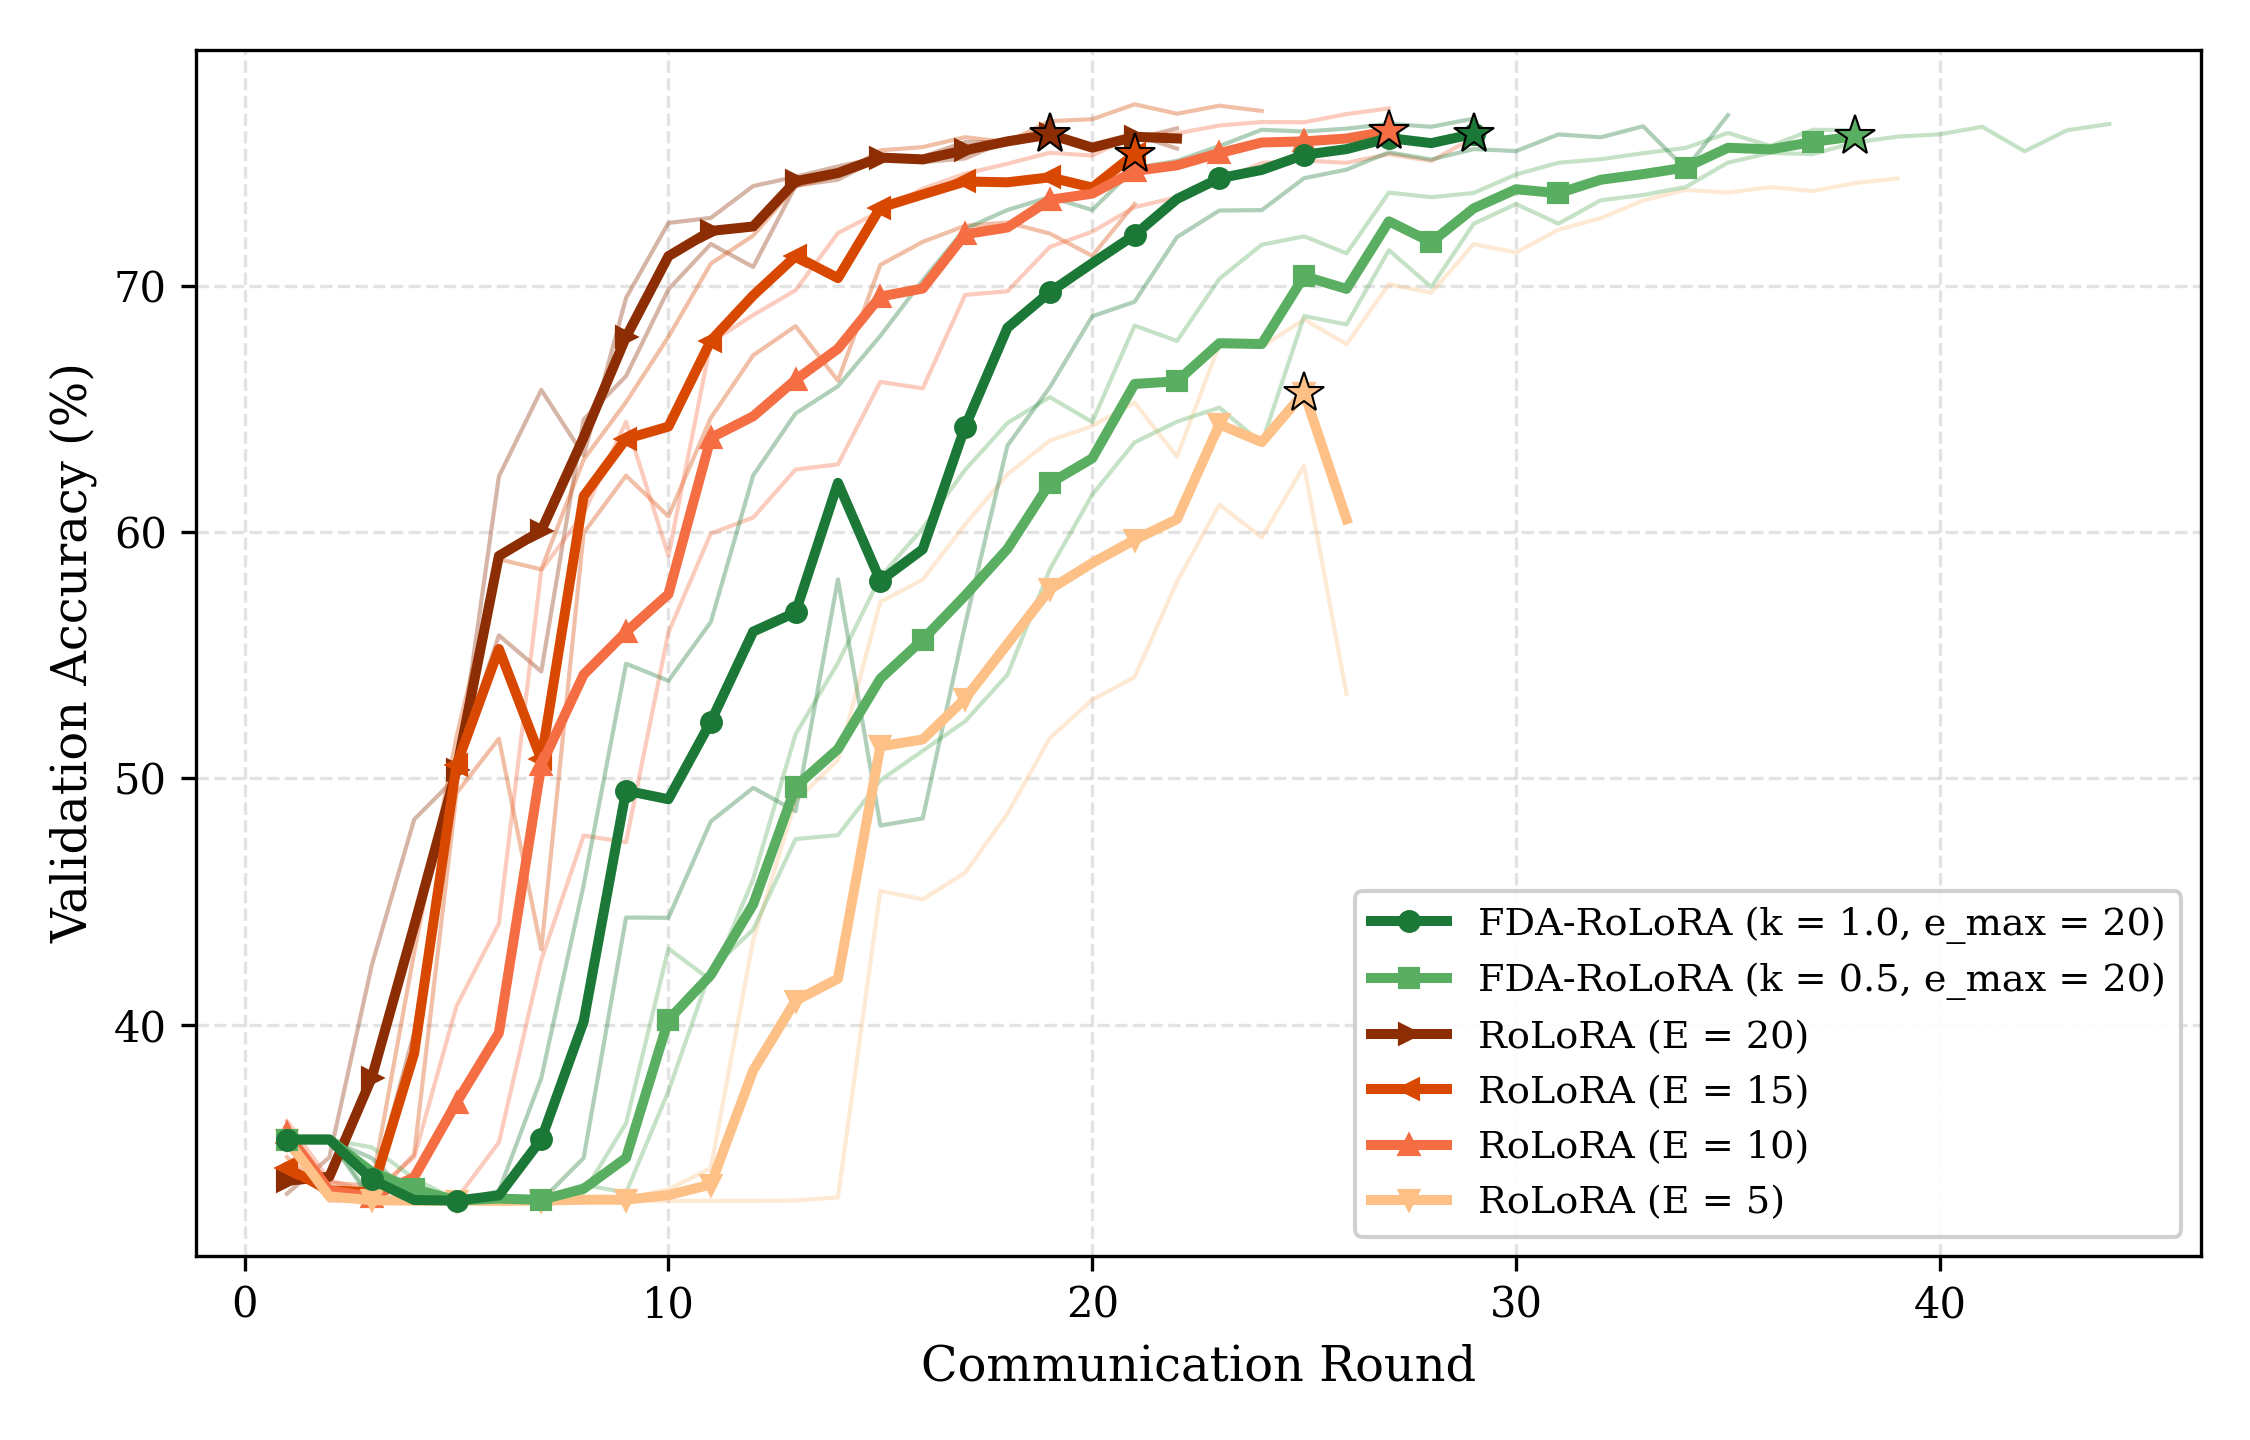
\includegraphics[width=\textwidth,height=4.9cm,keepaspectratio]{figures/telemetry/01_MNLI_C20_R50_LR0.1_1_accuracy.png}
            \vspace{2pt}
            \par{\footnotesize \textbf{(a)} Validation Accuracy}
        \end{minipage}\hfill
        \begin{minipage}[b]{0.485\textwidth}
            \centering
            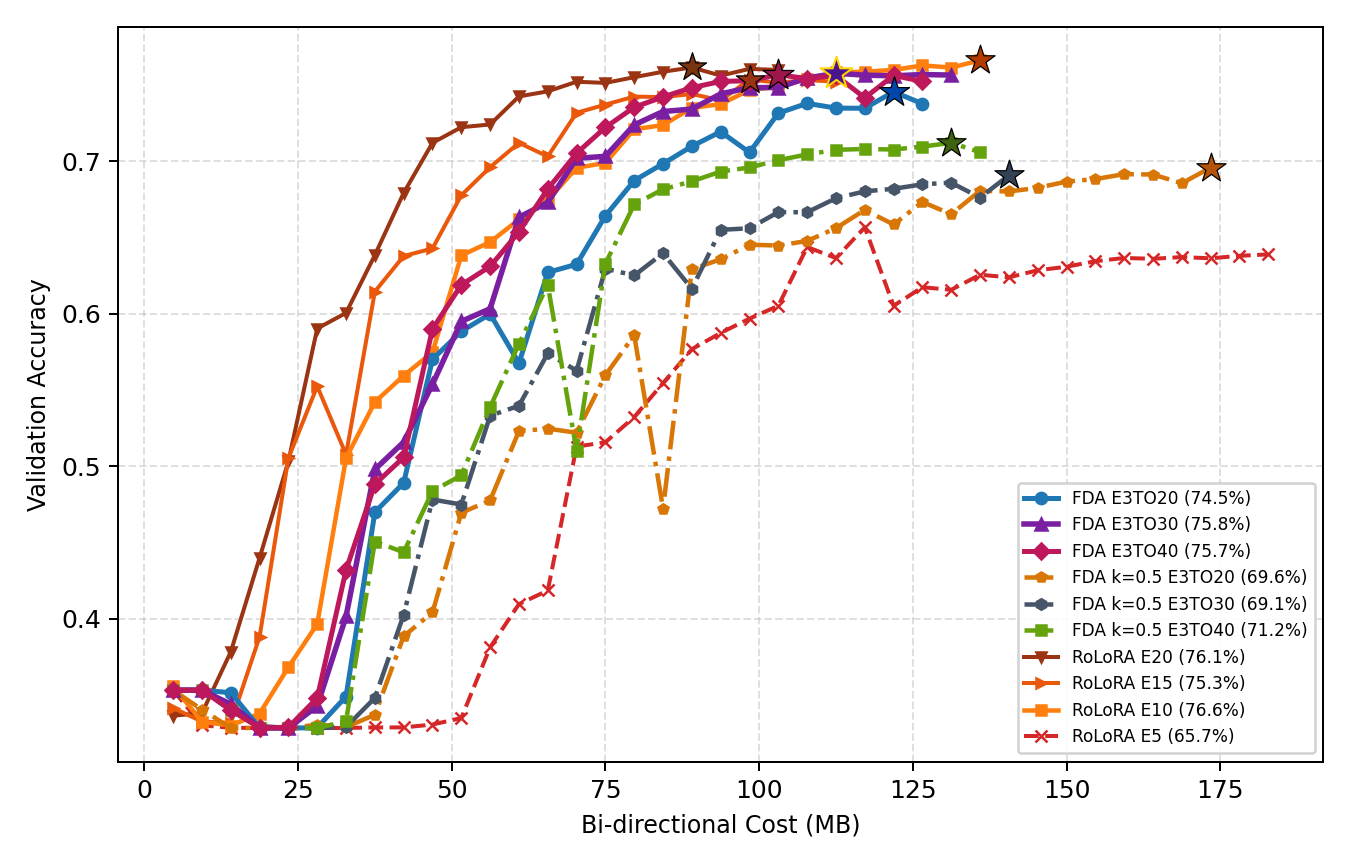
\includegraphics[width=\textwidth,height=4.9cm,keepaspectratio]{figures/telemetry/01_MNLI_C20_R50_LR0.1_4_accuracy_vs_cost.png}
            \vspace{2pt}
            \par{\footnotesize \textbf{(b)} Accuracy vs. Communication (MB)}
        \end{minipage}

        \vspace{0.6em}
        \begin{minipage}[b]{0.485\textwidth}
            \centering
            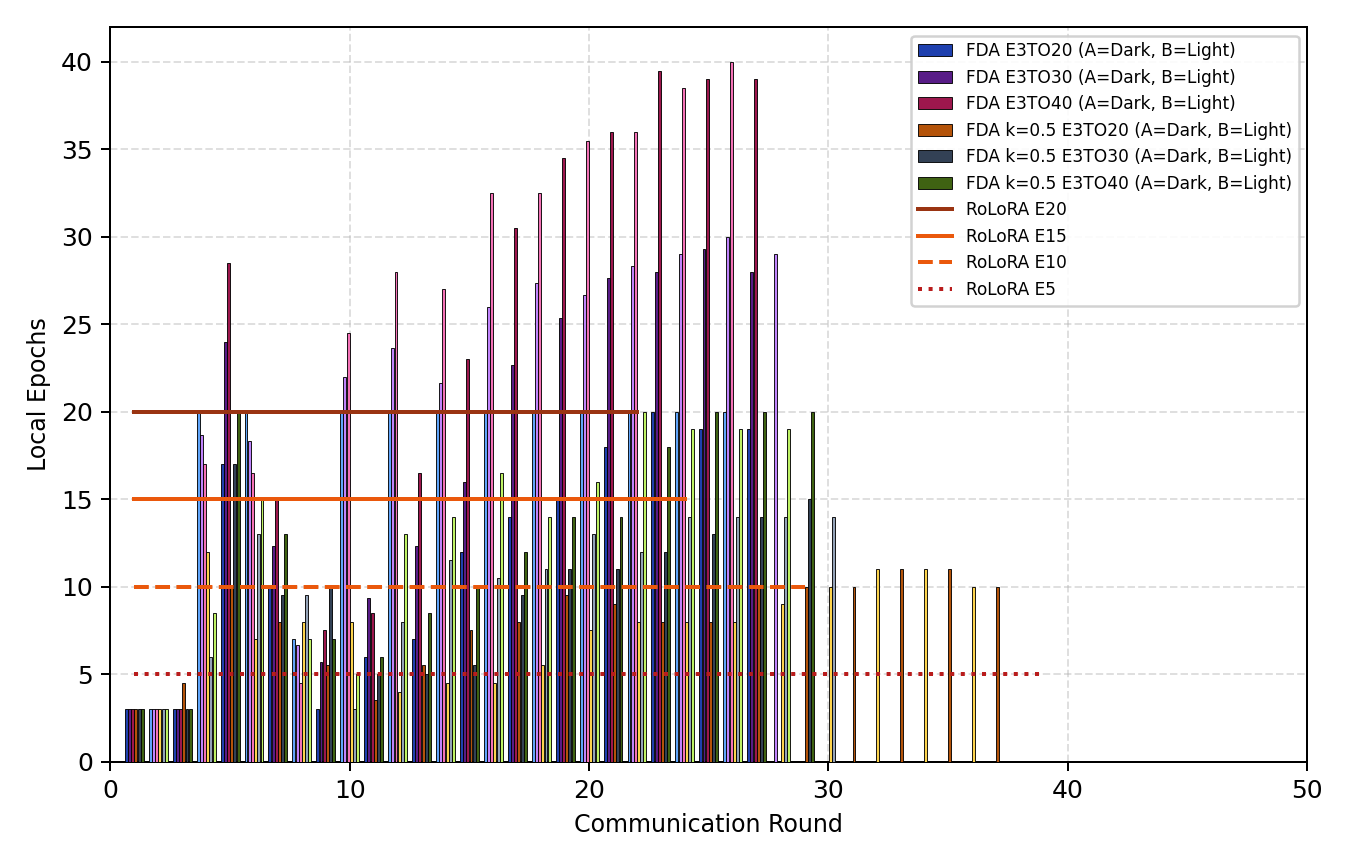
\includegraphics[width=\textwidth,height=4.9cm,keepaspectratio]{figures/telemetry/01_MNLI_C20_R50_LR0.1_2_allocated_epochs.png}
            \vspace{2pt}
            \par{\footnotesize \textbf{(c)} Dynamic Local Epochs ($\bar{e}$)}
        \end{minipage}\hfill
        \begin{minipage}[b]{0.485\textwidth}
            \centering
            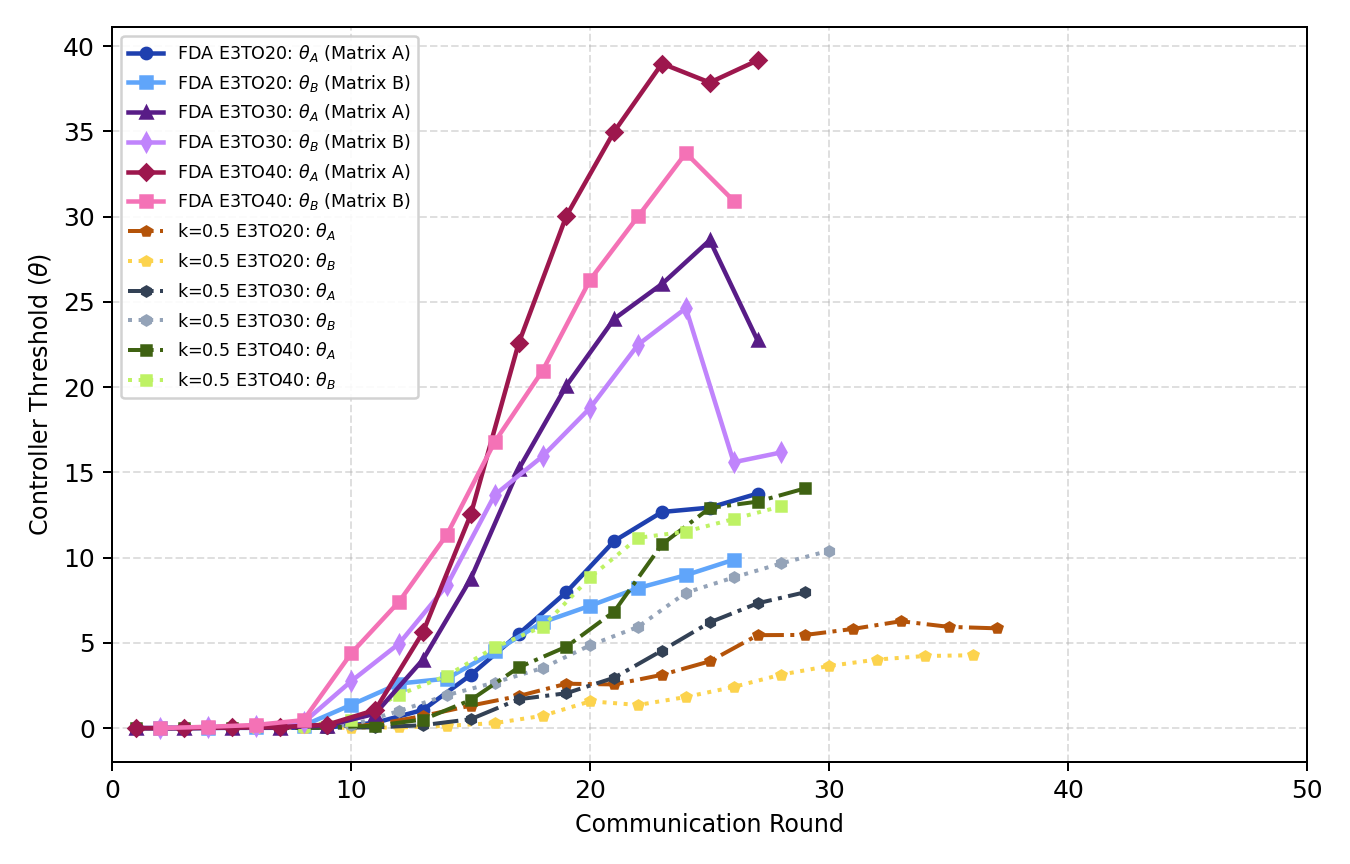
\includegraphics[width=\textwidth,height=4.9cm,keepaspectratio]{figures/telemetry/01_MNLI_C20_R50_LR0.1_5_fda_threshold.png}
            \vspace{2pt}
            \par{\footnotesize \textbf{(d)} Factor Thresholds ($\theta_A, \theta_B$)}
        \end{minipage}

        \vspace{0.6em}
        \begin{minipage}[b]{0.485\textwidth}
            \centering
            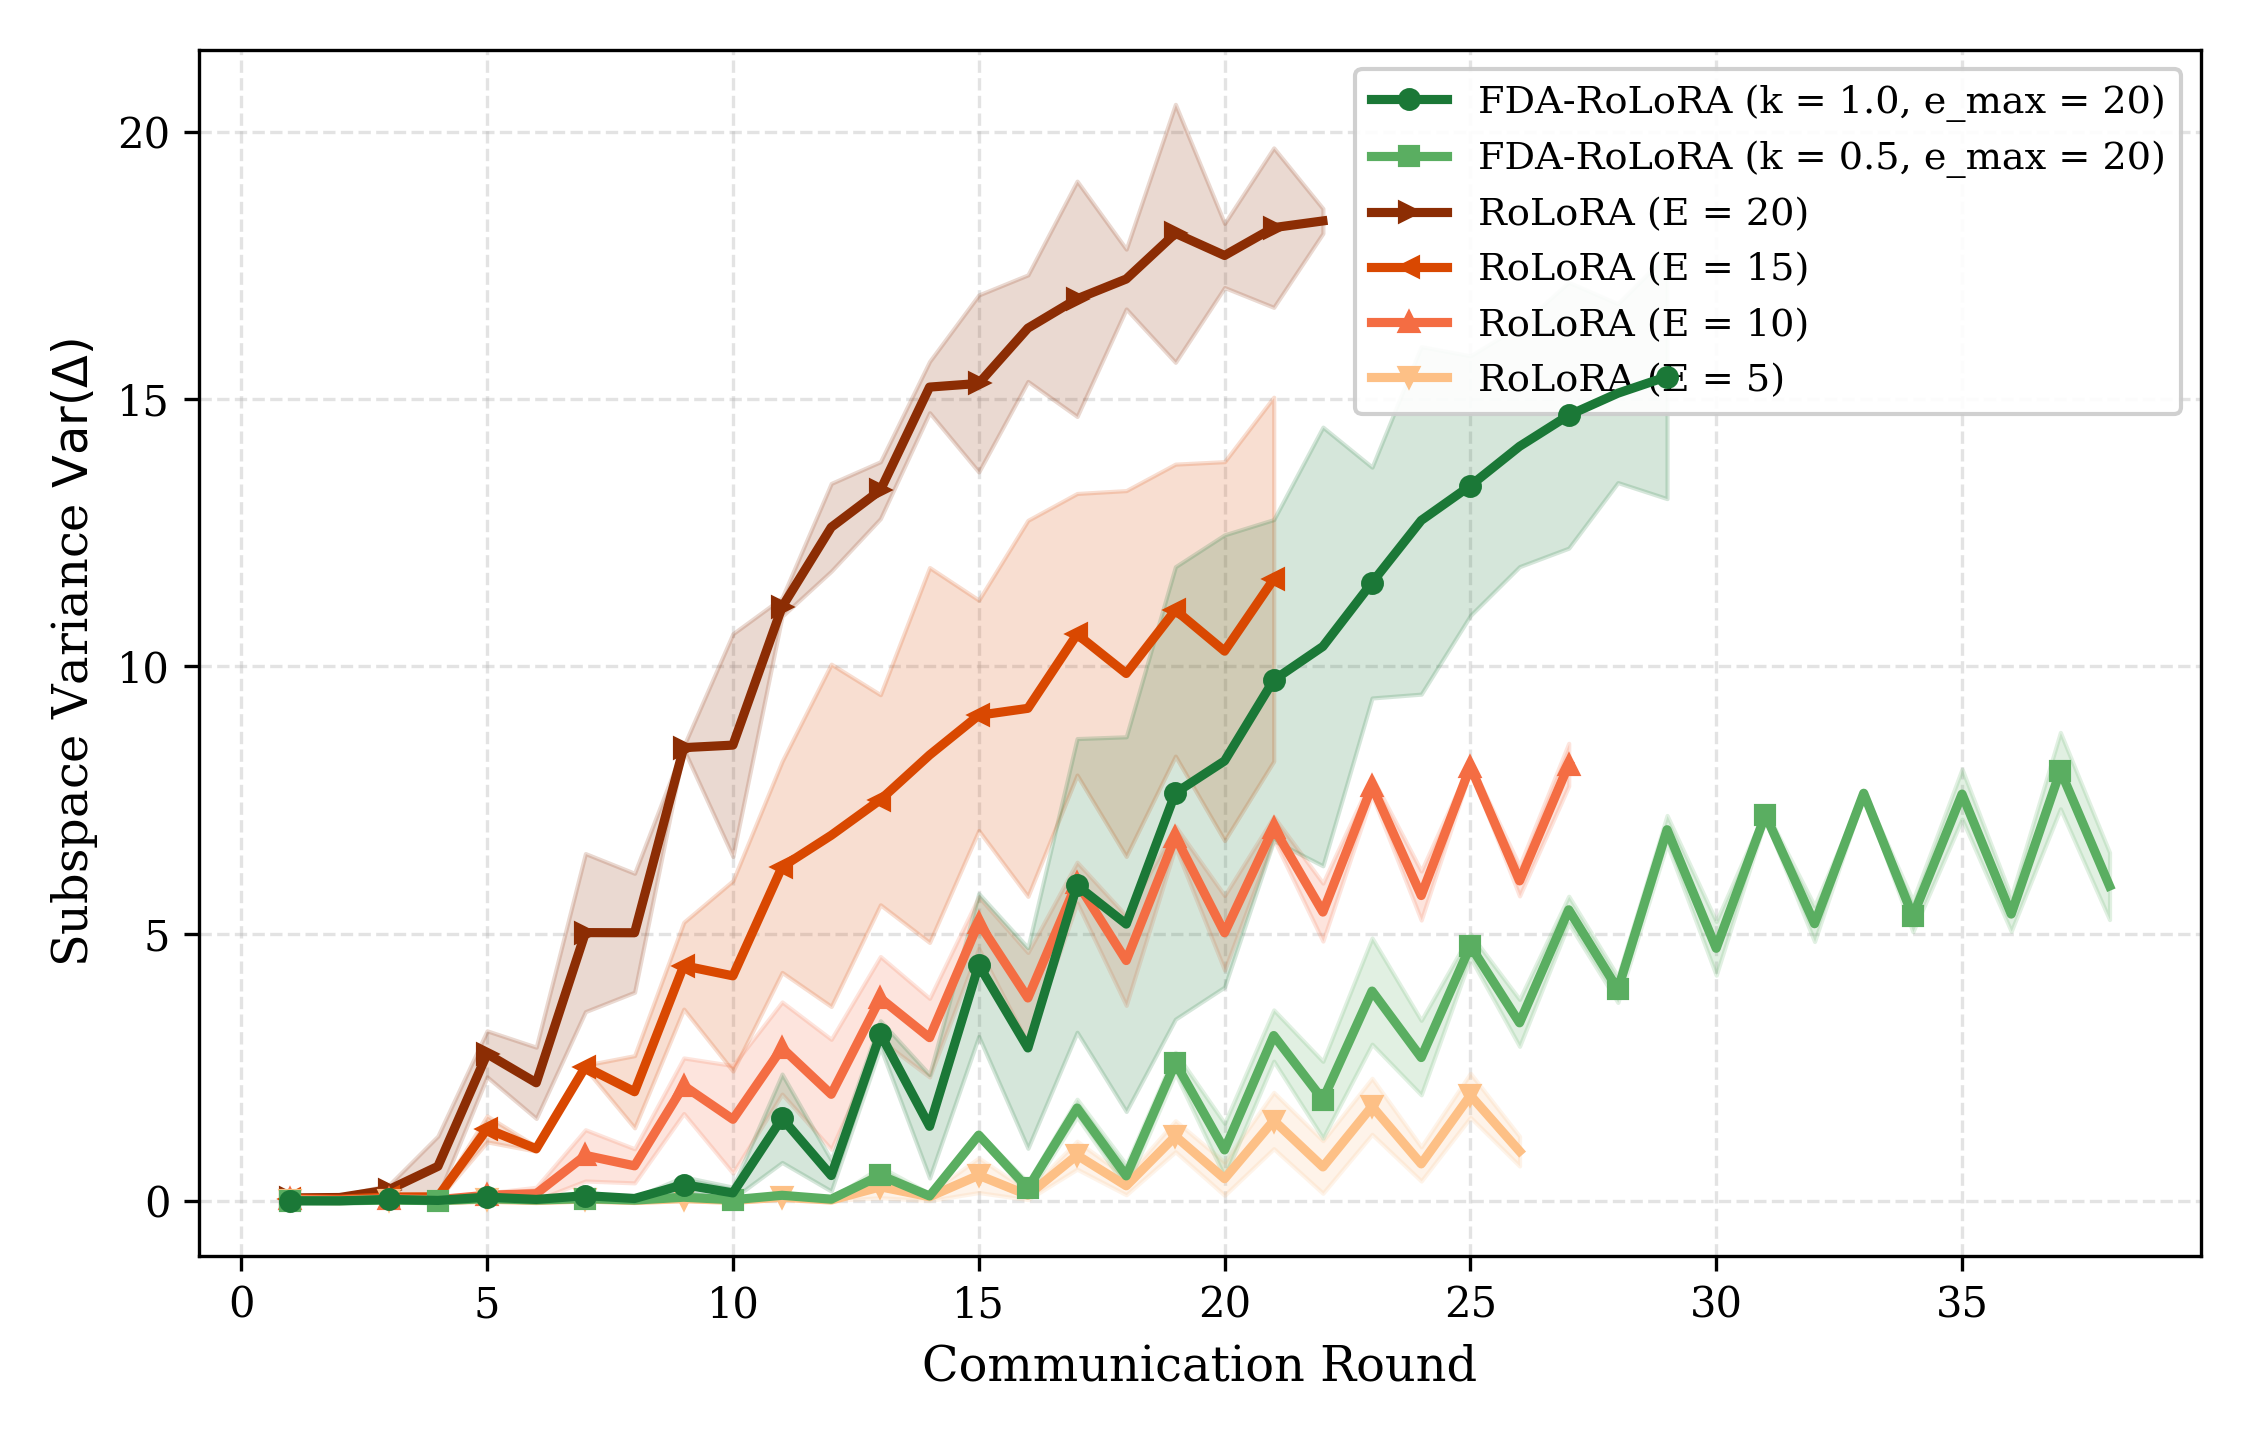
\includegraphics[width=\textwidth,height=4.9cm,keepaspectratio]{figures/telemetry/01_MNLI_C20_R50_LR0.1_3_client_variance.png}
            \vspace{2pt}
            \par{\footnotesize \textbf{(e)} Subspace Coordinate Variance}
        \end{minipage}\hfill
        \begin{minipage}[b]{0.485\textwidth}
            \centering
            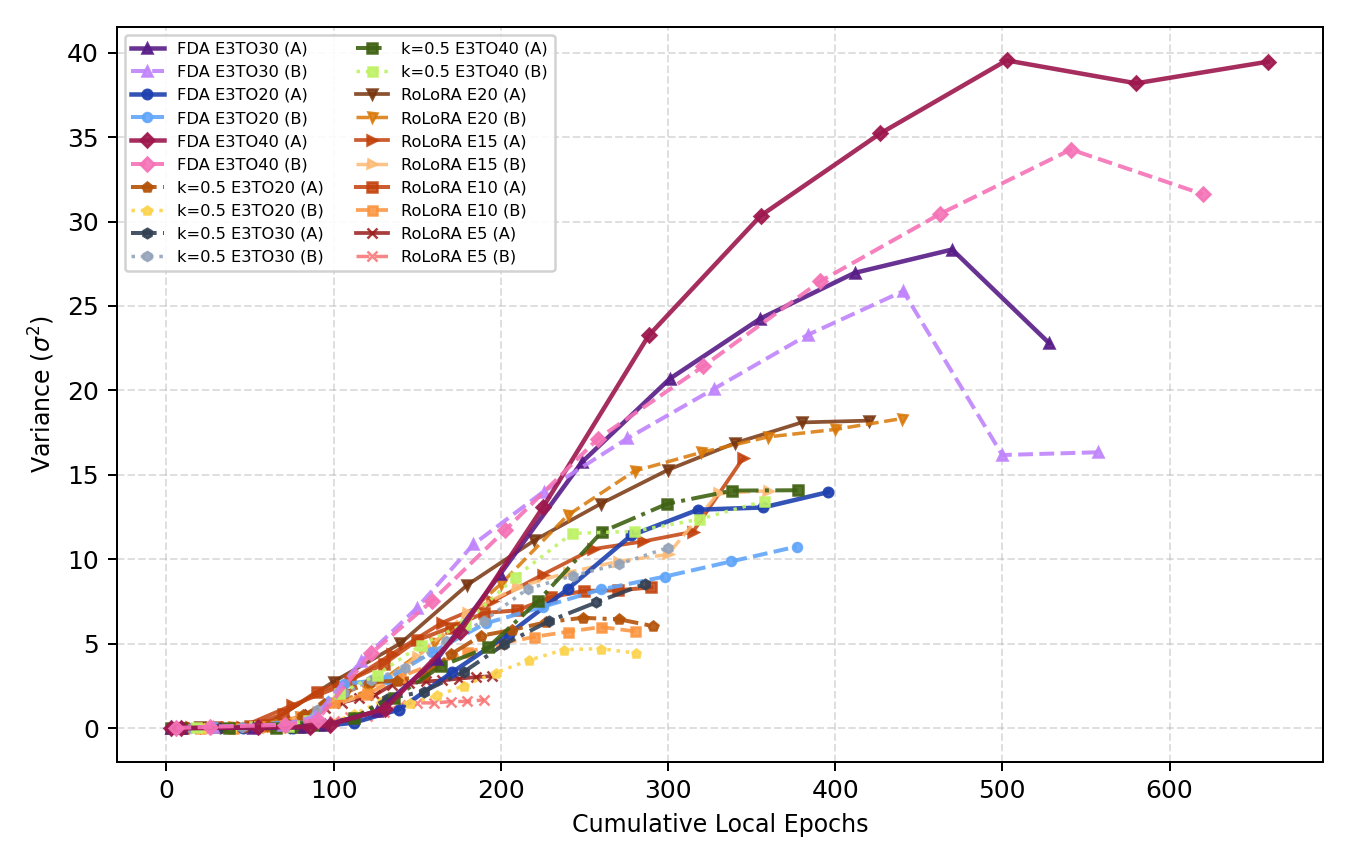
\includegraphics[width=\textwidth,height=4.9cm,keepaspectratio]{figures/telemetry/01_MNLI_C20_R50_LR0.1_6_variance_vs_epoch.png}
            \vspace{2pt}
            \par{\footnotesize \textbf{(f)} Variance vs.\ Cumulative Local Epochs}
        \end{minipage}

        \vspace{0.6em}
        \caption{Multi-panel optimization telemetry on MNLI ($C=20, R_{\max}=50, \eta_c=0.1, \alpha=1000.0$) comparing FDA-RoLoRA against static RoLoRA baselines under homogeneous consensus.}
        \label{fig:telemetry_mnli_c20_iid}
    \end{minipage}%
    }
\end{figure}

\begin{figure}[p]
    \centering
    \makebox[\textwidth][c]{%
    \begin{minipage}{1.06\textwidth}
        \begin{minipage}[b]{0.485\textwidth}
            \centering
            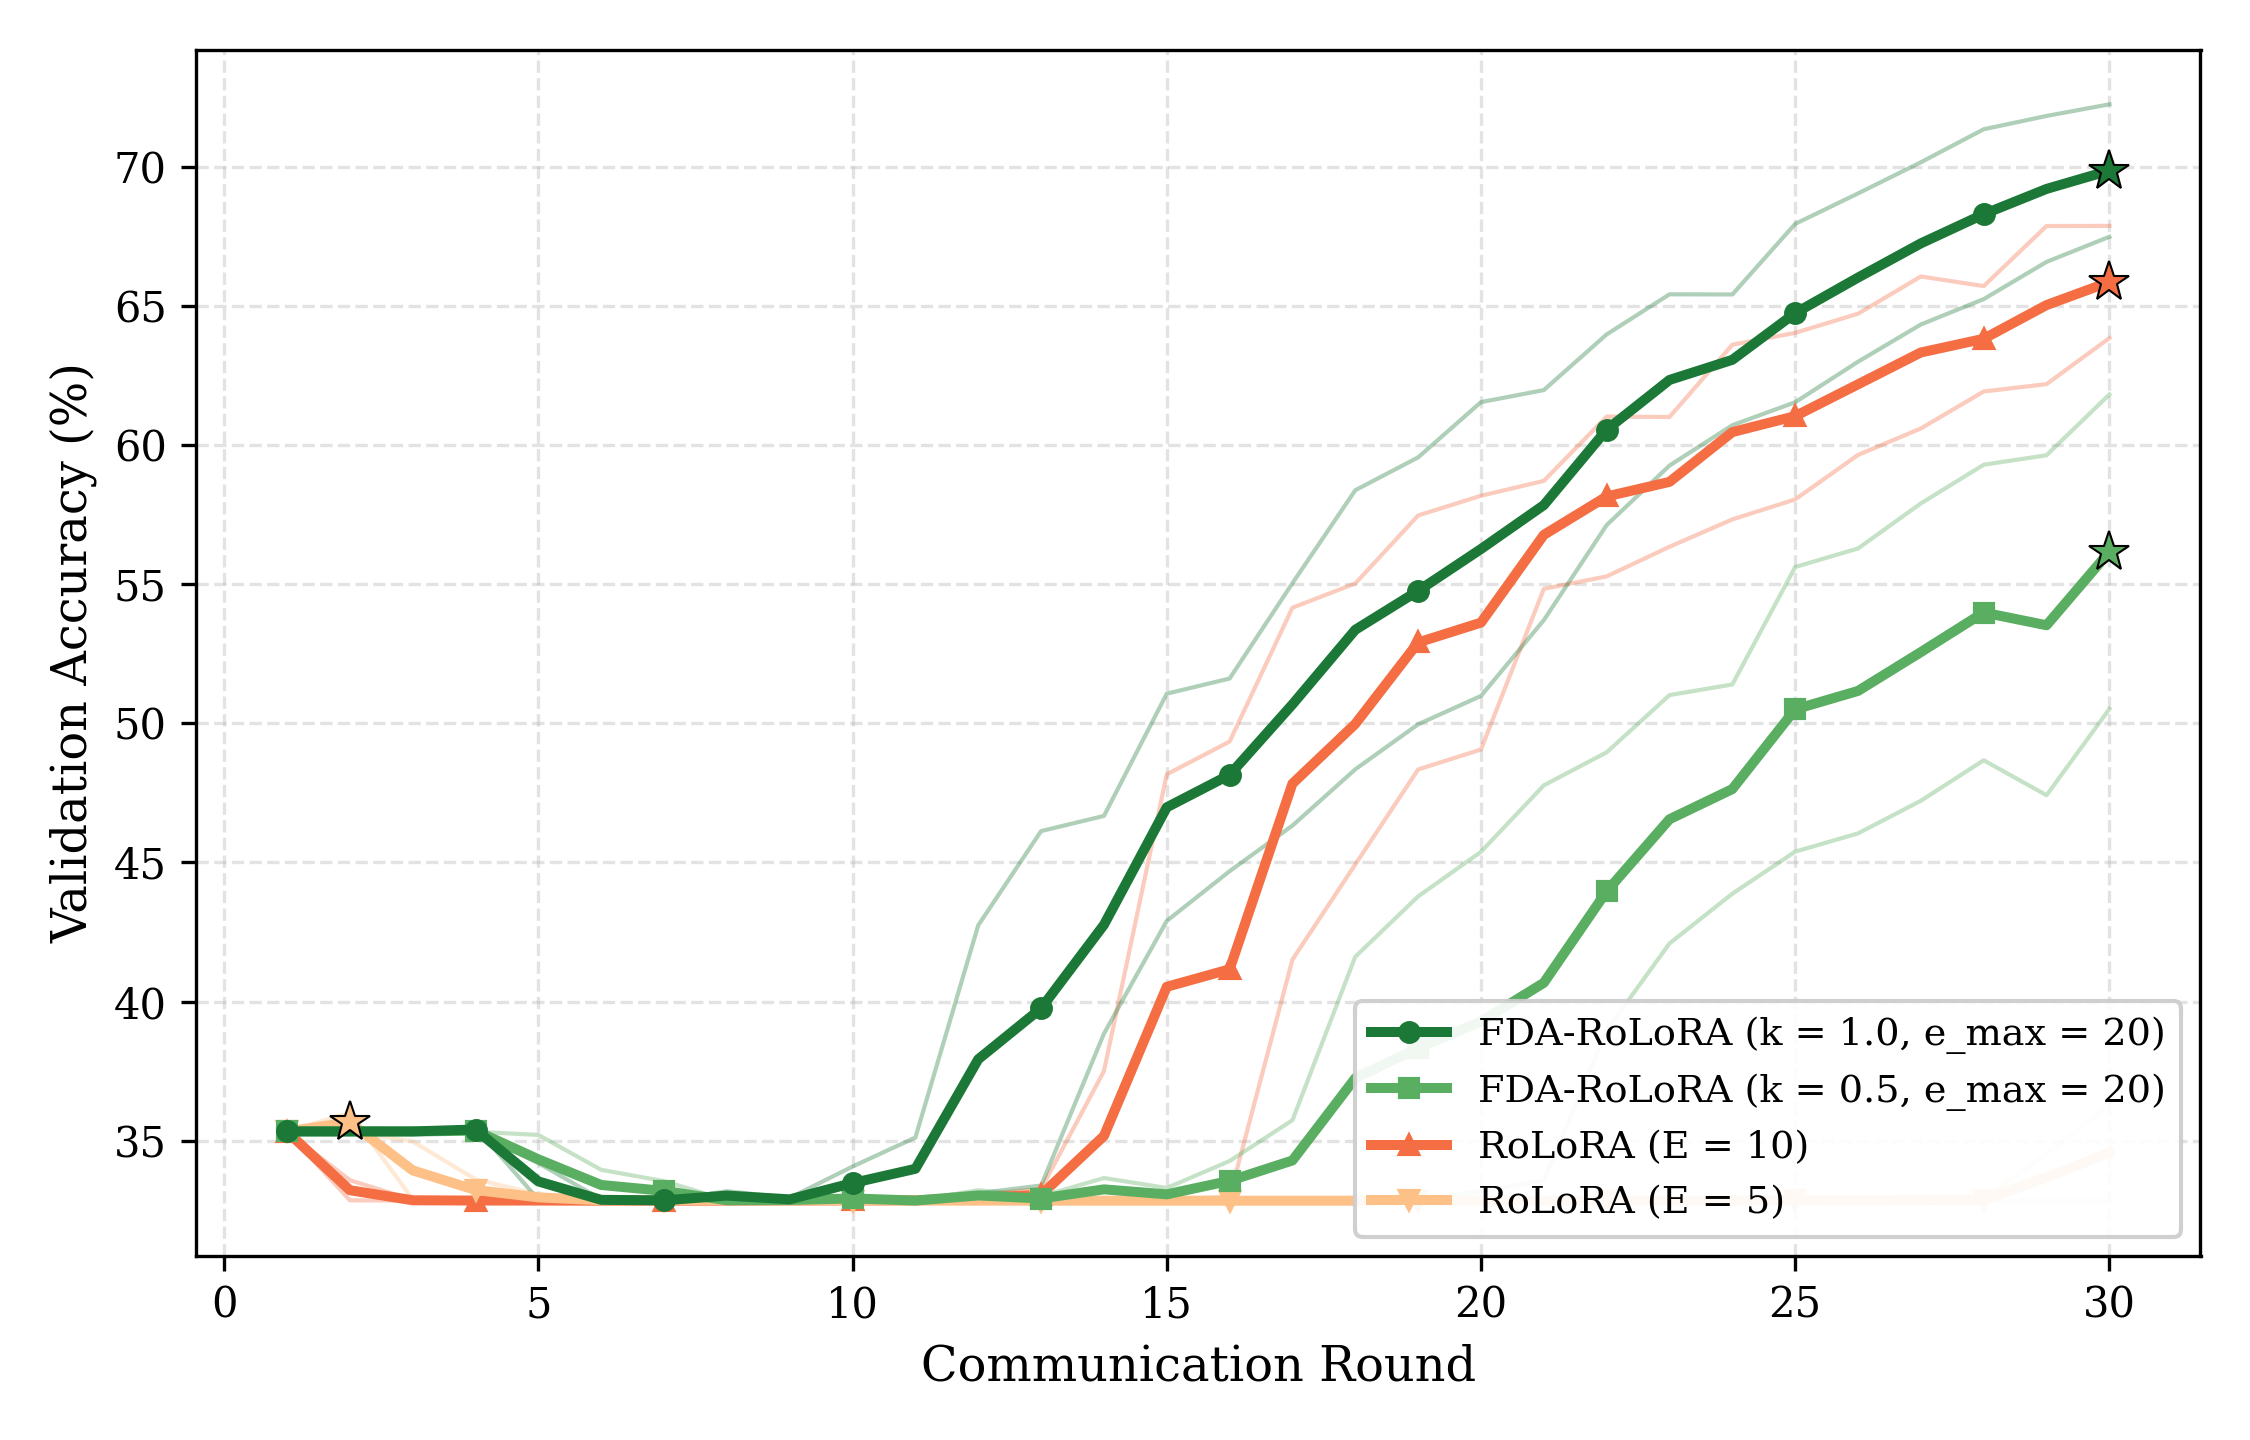
\includegraphics[width=\textwidth,height=4.9cm,keepaspectratio]{figures/telemetry/03_MNLI_C50_R30_LR0.1_1_accuracy.png}
            \vspace{2pt}
            \par{\footnotesize \textbf{(a)} Validation Accuracy}
        \end{minipage}\hfill
        \begin{minipage}[b]{0.485\textwidth}
            \centering
            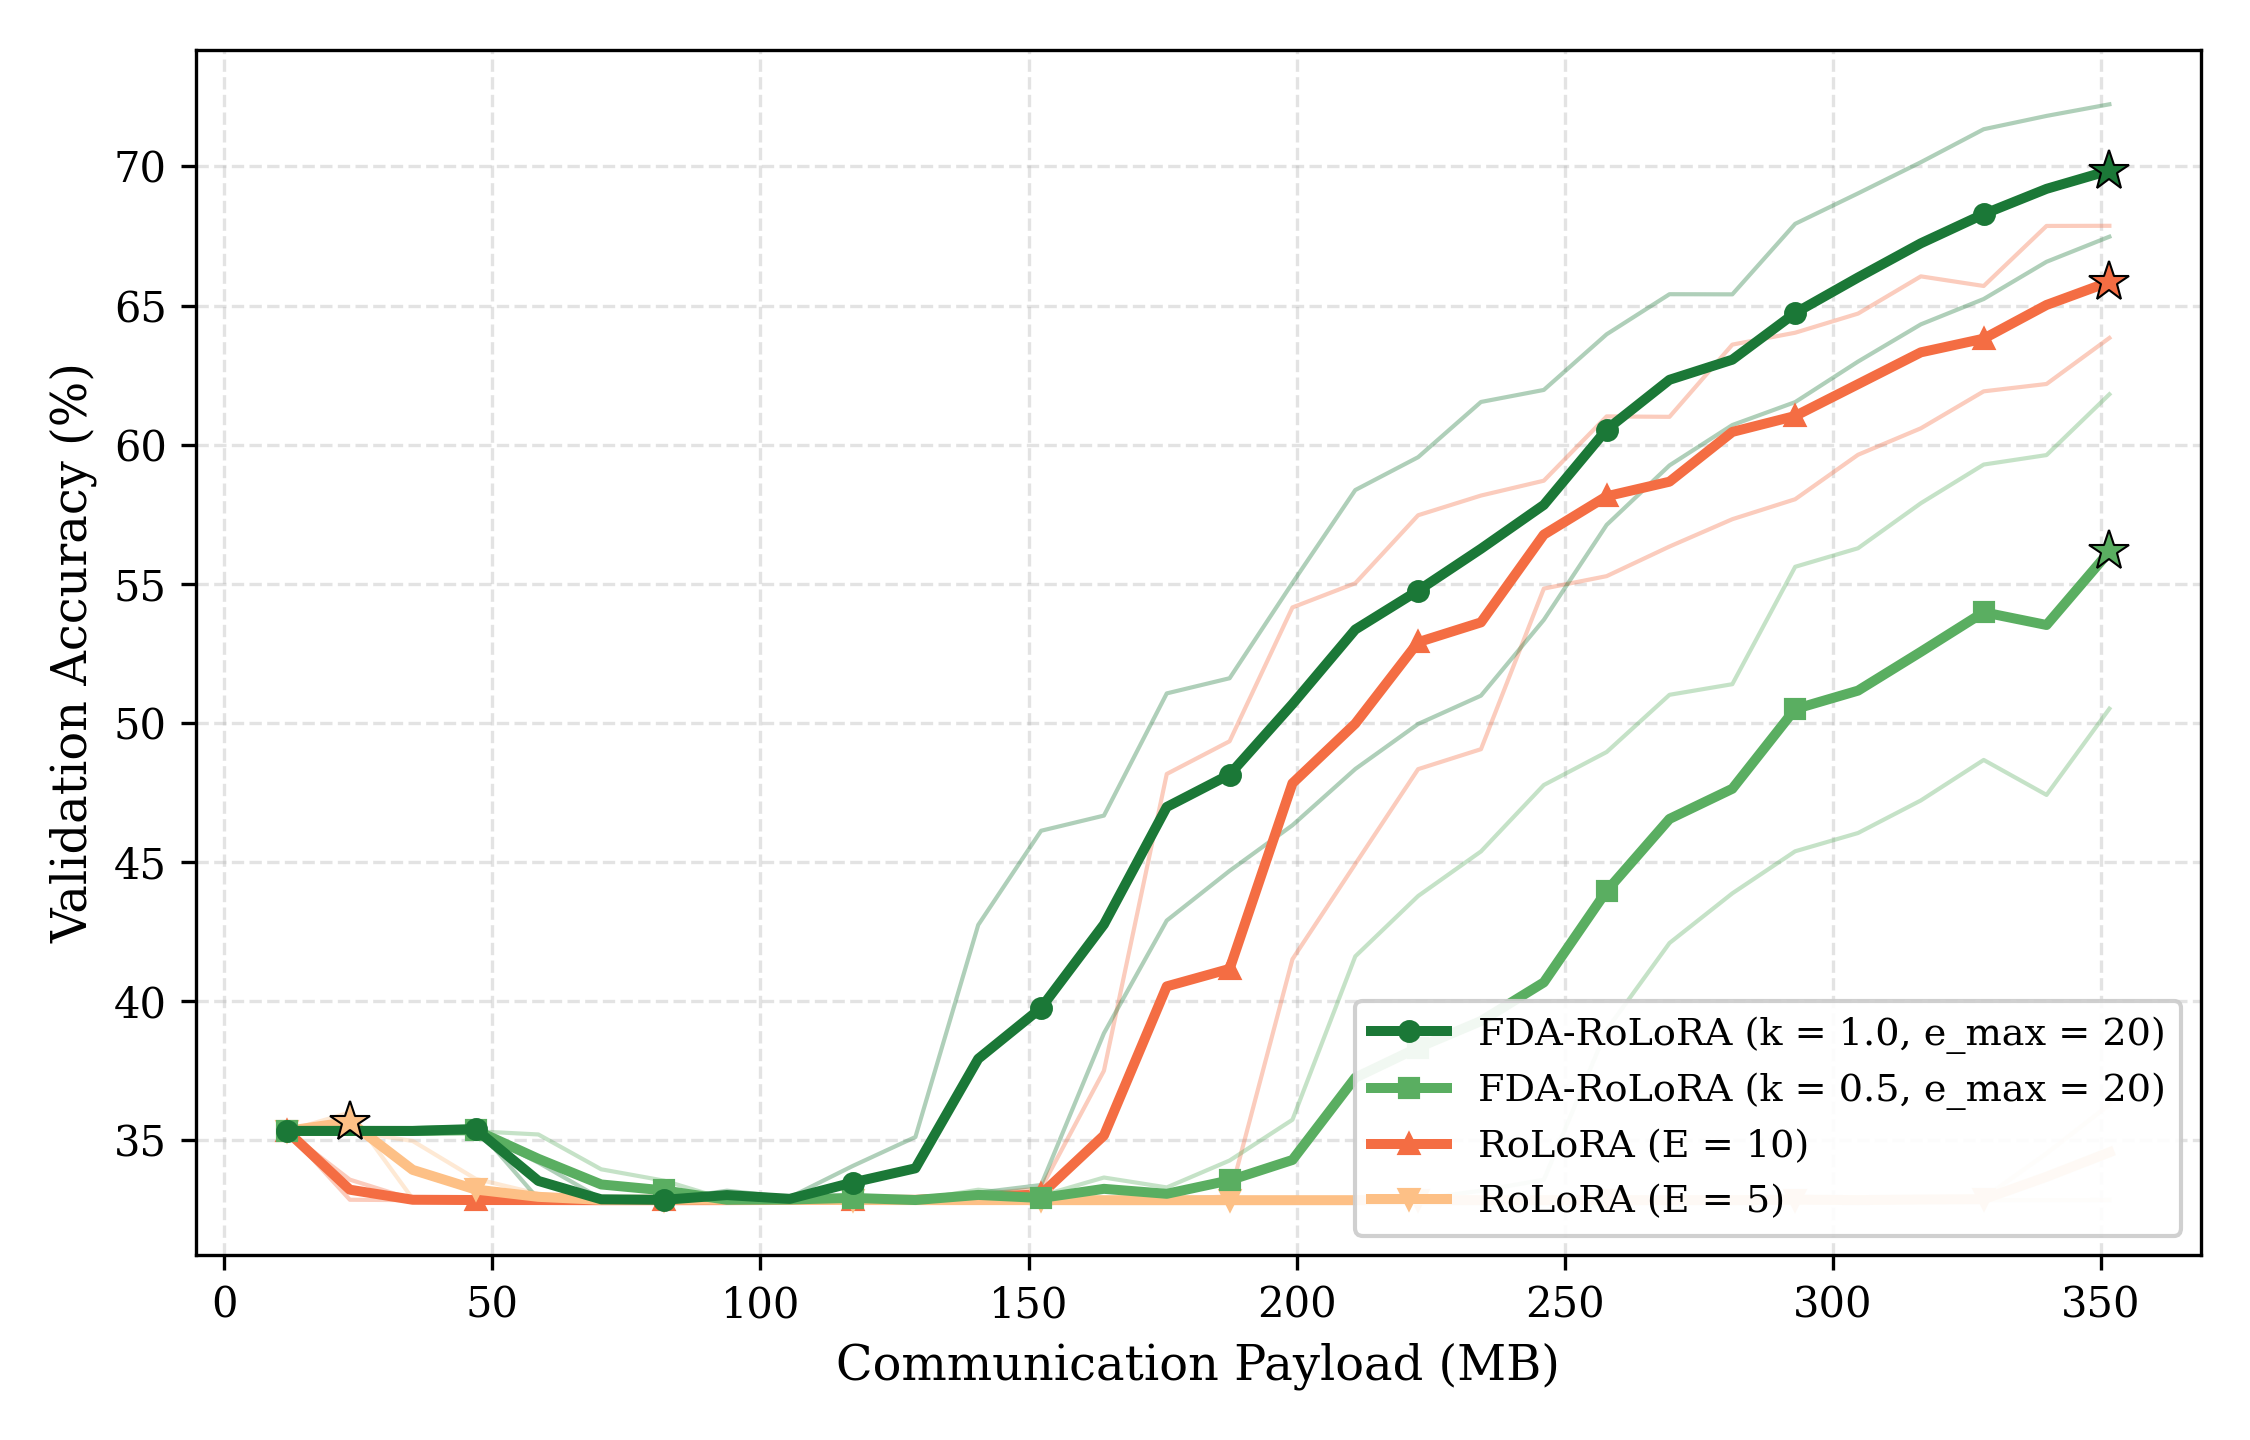
\includegraphics[width=\textwidth,height=4.9cm,keepaspectratio]{figures/telemetry/03_MNLI_C50_R30_LR0.1_4_accuracy_vs_cost.png}
            \vspace{2pt}
            \par{\footnotesize \textbf{(b)} Accuracy vs. Communication (MB)}
        \end{minipage}

        \vspace{0.6em}
        \begin{minipage}[b]{0.485\textwidth}
            \centering
            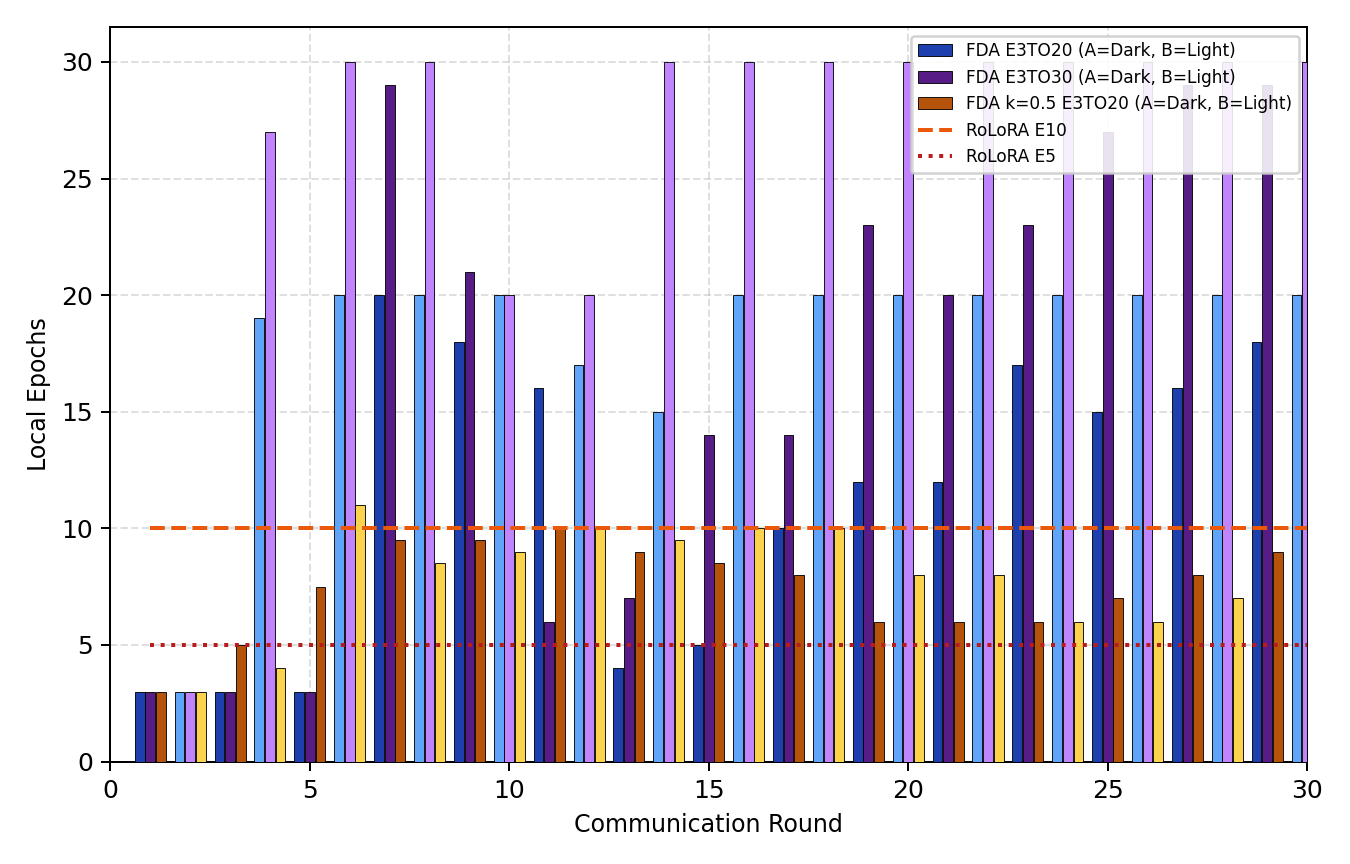
\includegraphics[width=\textwidth,height=4.9cm,keepaspectratio]{figures/telemetry/03_MNLI_C50_R30_LR0.1_2_allocated_epochs.png}
            \vspace{2pt}
            \par{\footnotesize \textbf{(c)} Dynamic Local Epochs ($\bar{e}$)}
        \end{minipage}\hfill
        \begin{minipage}[b]{0.485\textwidth}
            \centering
            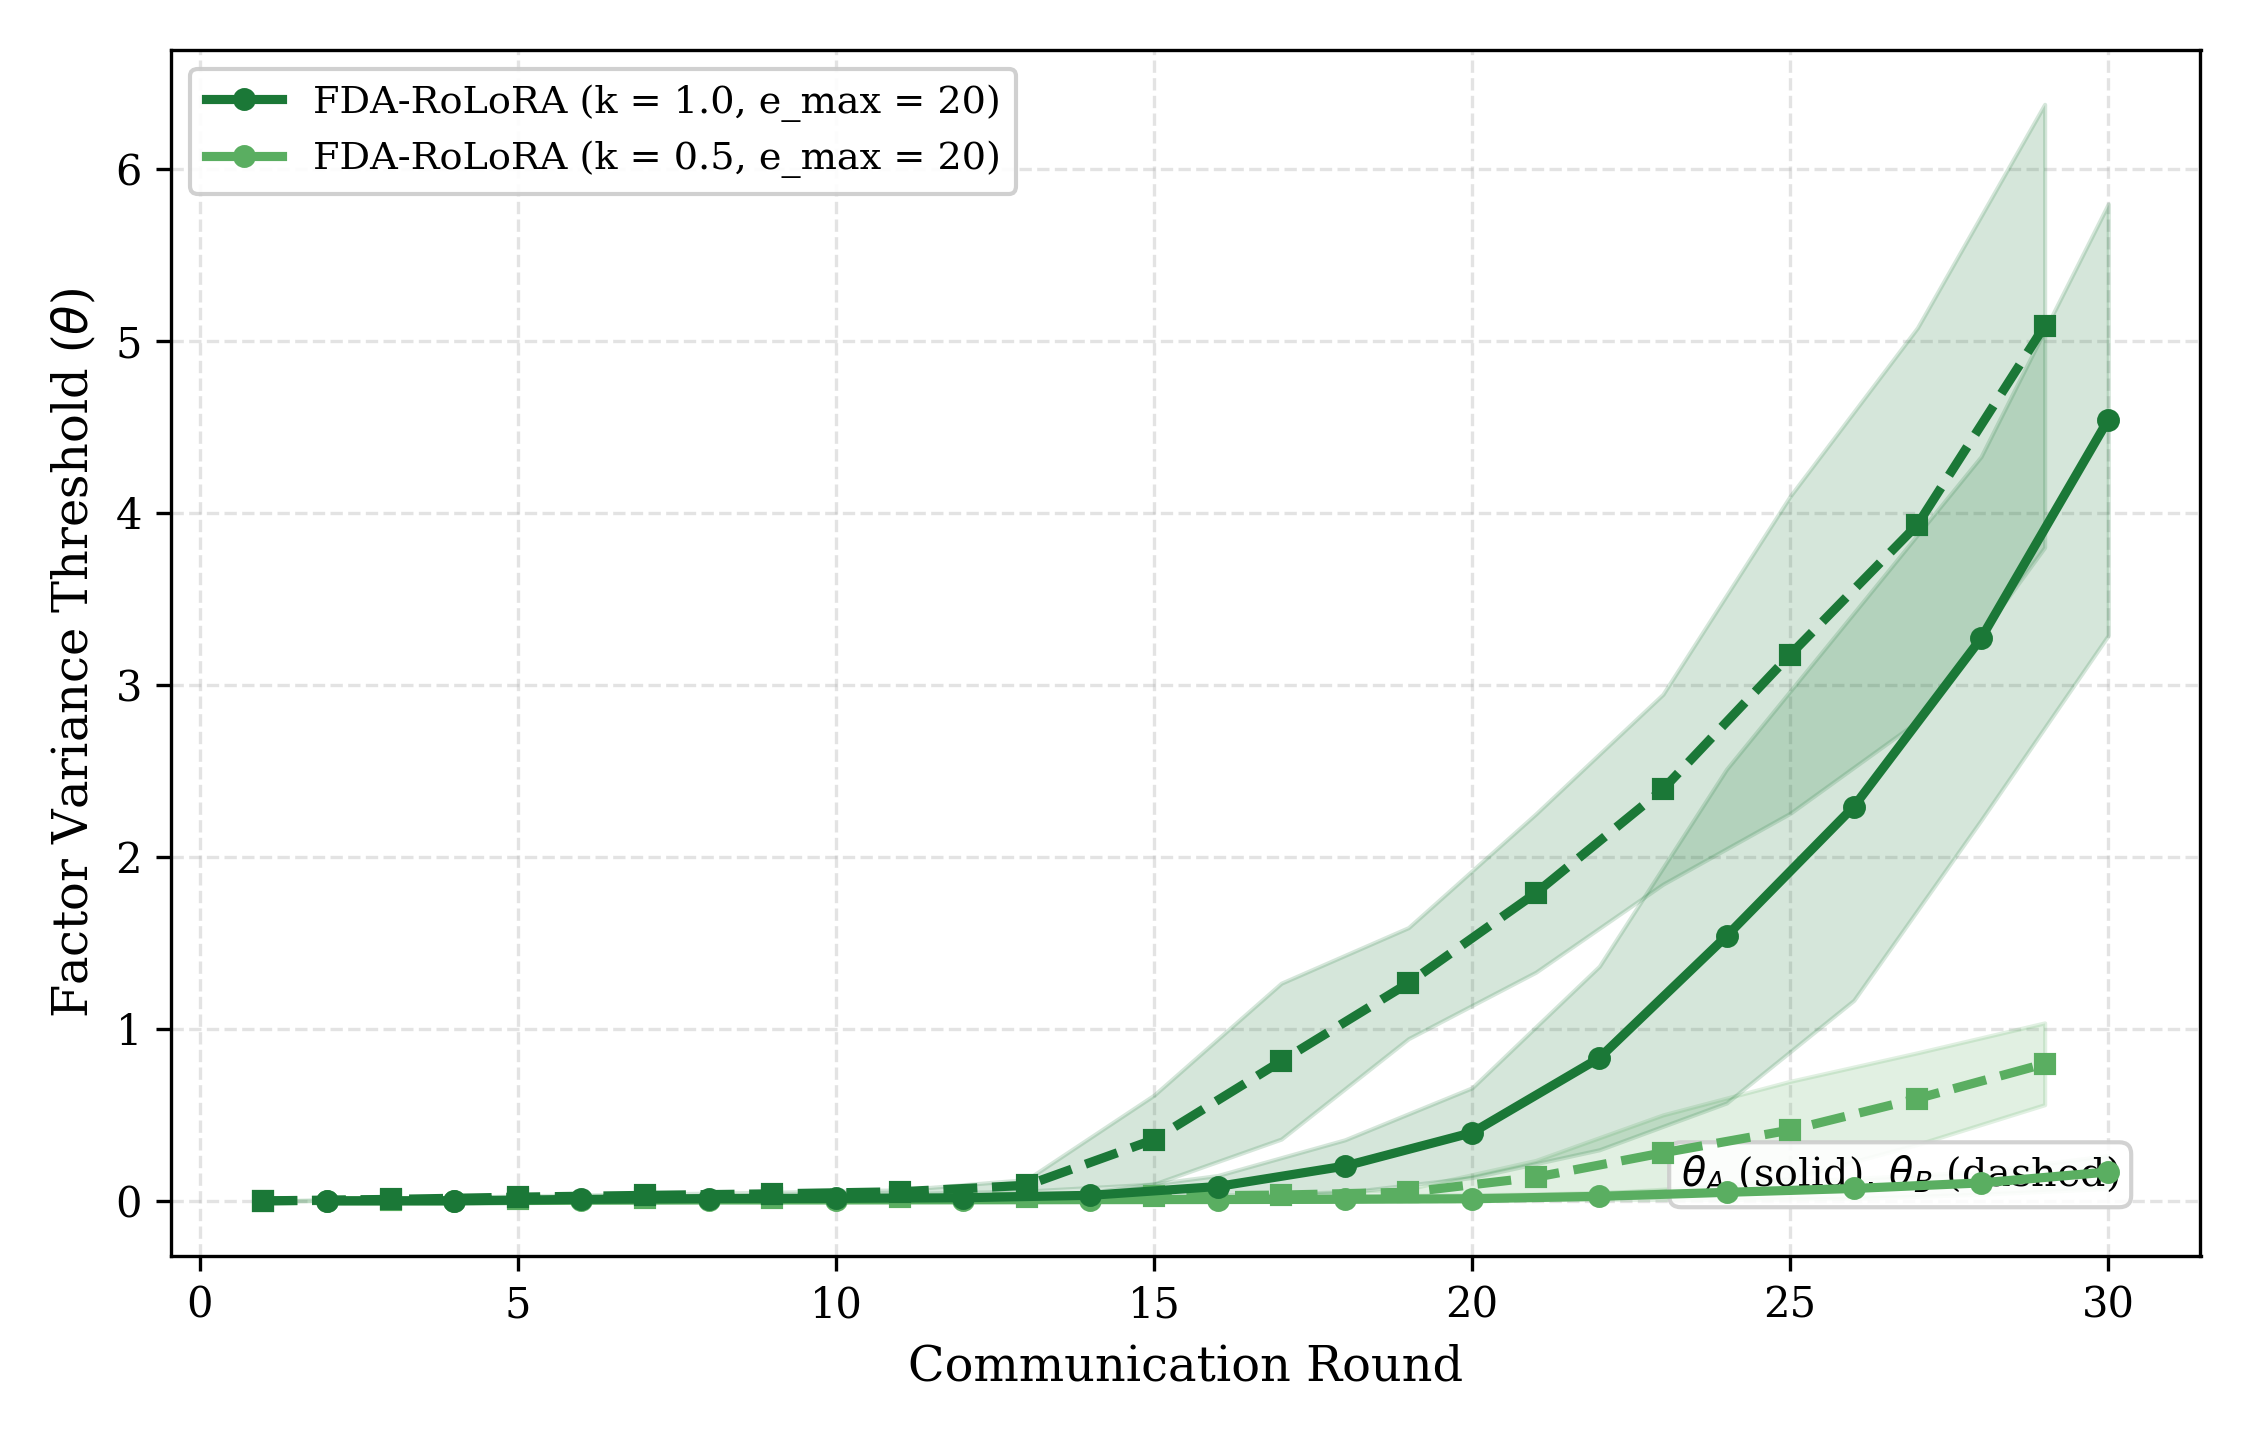
\includegraphics[width=\textwidth,height=4.9cm,keepaspectratio]{figures/telemetry/03_MNLI_C50_R30_LR0.1_5_fda_threshold.png}
            \vspace{2pt}
            \par{\footnotesize \textbf{(d)} Factor Thresholds ($\theta_A, \theta_B$)}
        \end{minipage}

        \vspace{0.6em}
        \begin{minipage}[b]{0.485\textwidth}
            \centering
            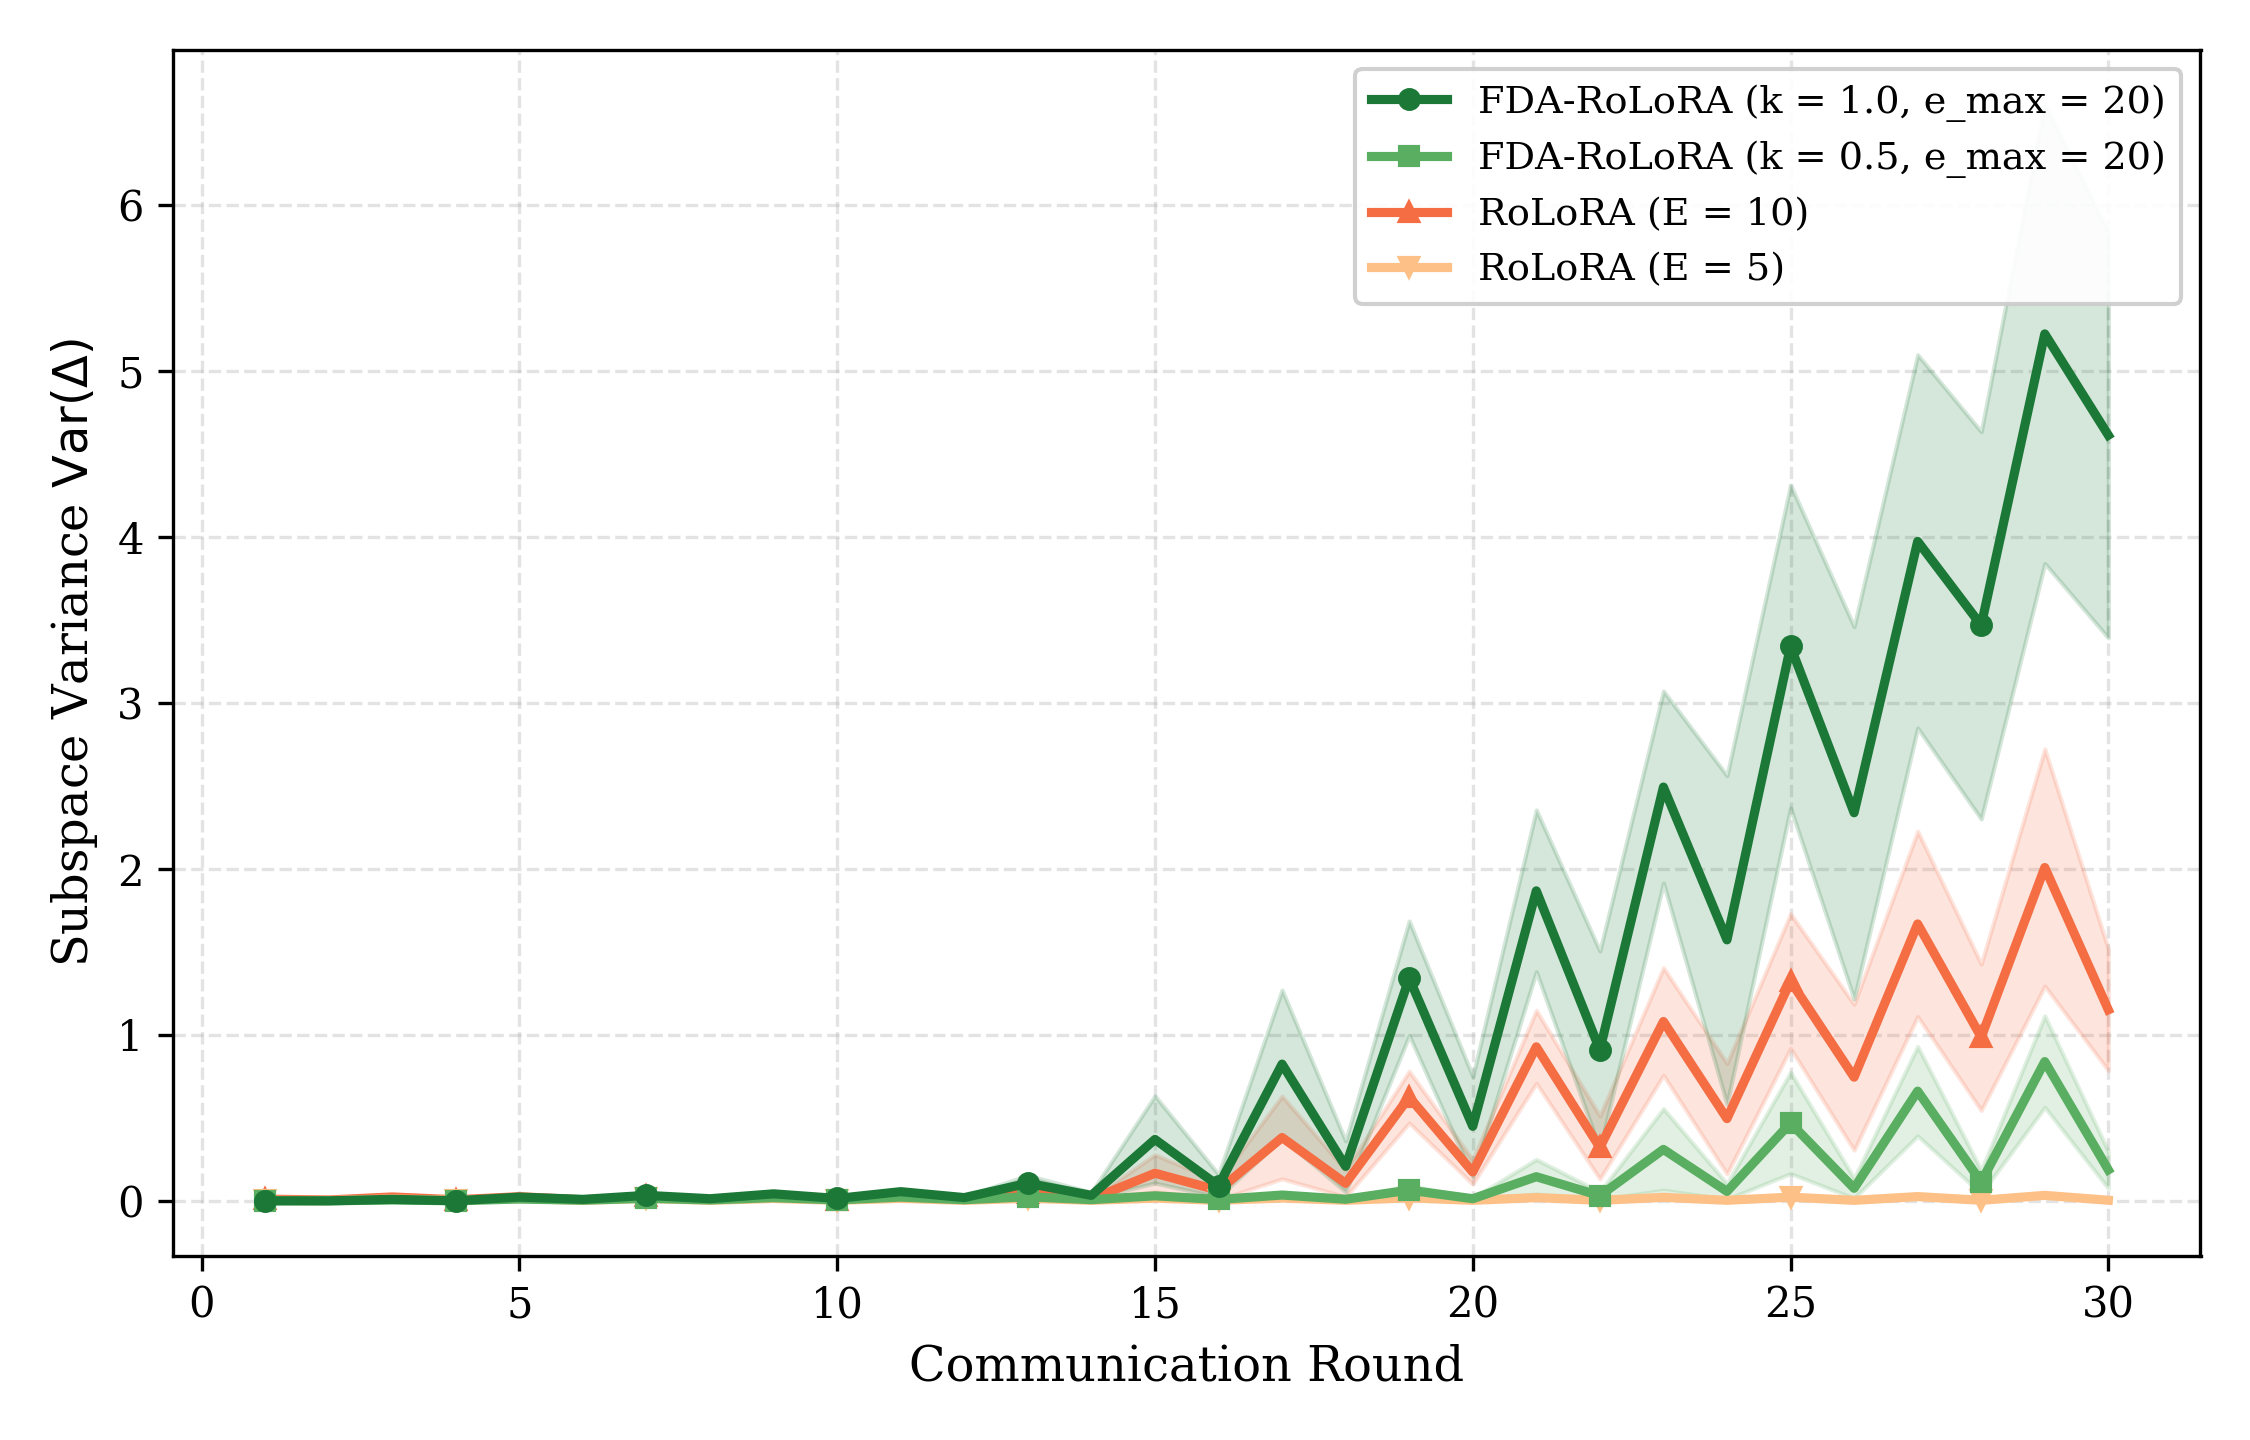
\includegraphics[width=\textwidth,height=4.9cm,keepaspectratio]{figures/telemetry/03_MNLI_C50_R30_LR0.1_3_client_variance.png}
            \vspace{2pt}
            \par{\footnotesize \textbf{(e)} Subspace Coordinate Variance}
        \end{minipage}\hfill
        \begin{minipage}[b]{0.485\textwidth}
            \centering
            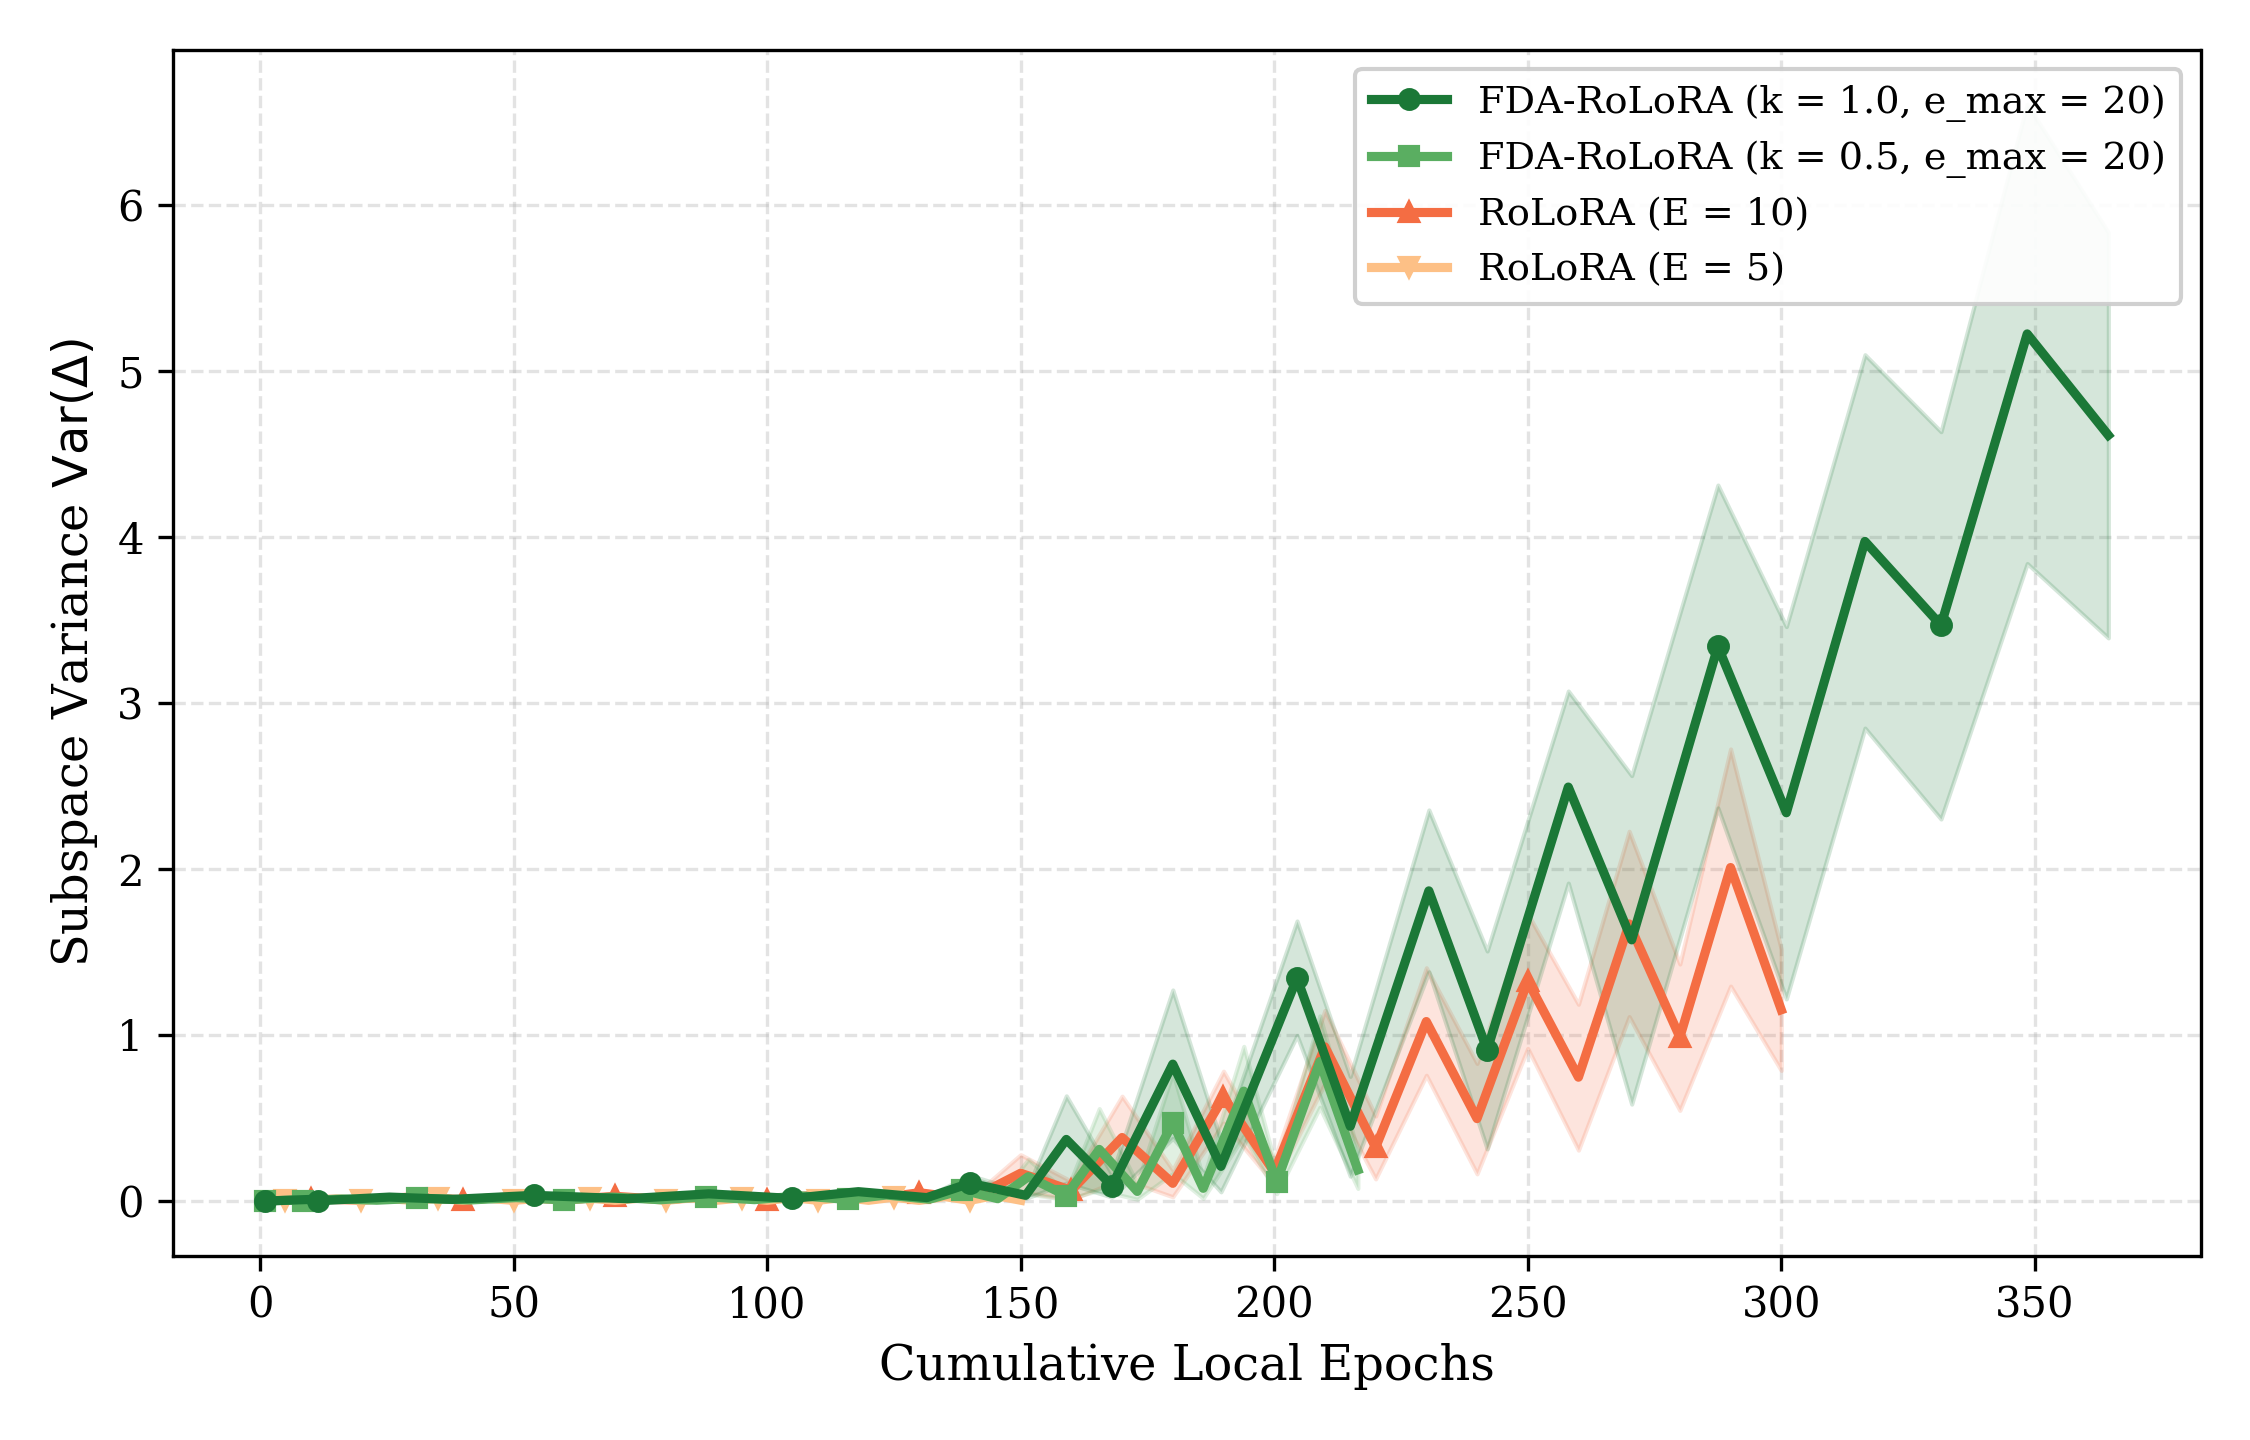
\includegraphics[width=\textwidth,height=4.9cm,keepaspectratio]{figures/telemetry/03_MNLI_C50_R30_LR0.1_6_variance_vs_epoch.png}
            \vspace{2pt}
            \par{\footnotesize \textbf{(f)} Variance vs.\ Cumulative Local Epochs}
        \end{minipage}

        \vspace{0.6em}
        \caption{Multi-panel optimization telemetry on MNLI ($C=50, R_{\max}=30, \eta_c=0.1, \alpha=1000.0$) under expanded cohort scale $C=50$.}
        \label{fig:telemetry_mnli_c50_iid}
    \end{minipage}%
    }
\end{figure}

\paragraph{QNLI:}
Figures~\ref{fig:telemetry_qnli_c20_iid} and \ref{fig:telemetry_qnli_c50_iid} depict optimization dynamics on binary question-answering inference under homogeneous consensus across the six telemetry panels. On $C=20$ (Figure~\ref{fig:telemetry_qnli_c20_iid}), FDA-RoLoRA ($k=1.0$) reaches a peak validation accuracy of $83.14\%$ (Panel a), compared with $81.83\%$ for RoLoRA $E=10$. However, it uses more communication ($77.3\,\text{MB}$ vs.\ $46.9\,\text{MB}$), and its final accuracy ($67.63 \pm 22.28\%$) is lower and less stable than its peak, because one seed ended at $51.9\%$. Dynamic local epochs (Panel c) stabilize at $\bar{e} = 9.85$ per round under $k=1.0$ (and $\bar{e} = 6.91$ under $k=0.5$), below the $k=1.0$ setpoint of 20. Threshold telemetry (Panel d) shows stable monotonic adaptation, preserving separate operational scales for $\theta_A$ and $\theta_B$. Drift variance at round synchronization (Panel e) is kept minimal ($\bar{\nu} \approx 1.11$).

On scaled cohorts of $C=50$ clients (Figure~\ref{fig:telemetry_qnli_c50_iid}), FDA-RoLoRA ($k=1.0$) reaches competitive peak accuracy ($82.77\%$) and triggers early stopping at round 21 ($246.1\,\text{MB}$) versus 24.5 rounds ($287.1\,\text{MB}$) for static RoLoRA $E=10$ (Panel a \& b). Inter-client drift variance (Panel e) averages only $\bar{\nu} = 0.707$.
\begin{figure}[p]
    \centering
    \makebox[\textwidth][c]{%
    \begin{minipage}{1.06\textwidth}
        \begin{minipage}[b]{0.485\textwidth}
            \centering
            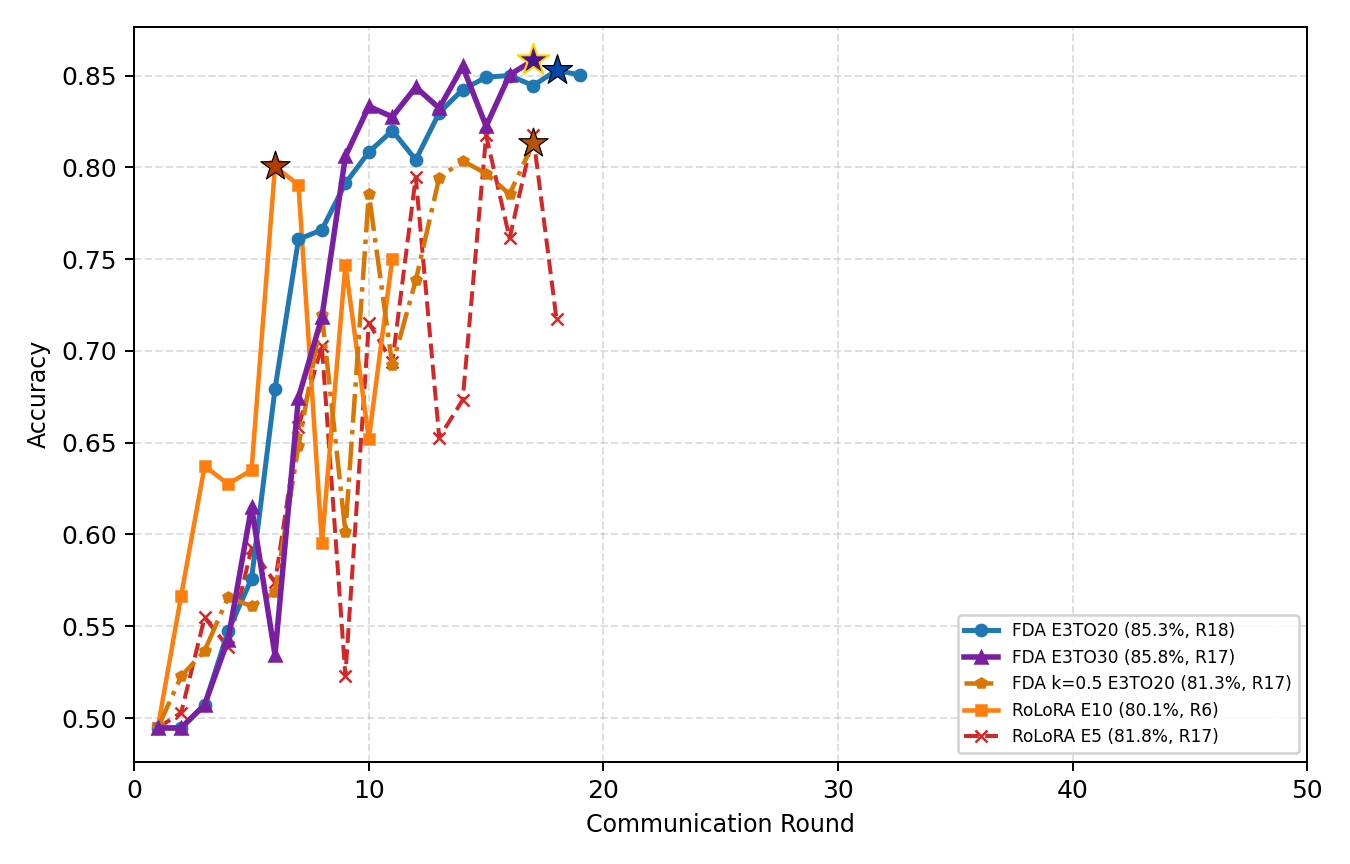
\includegraphics[width=\textwidth,height=4.9cm,keepaspectratio]{figures/telemetry/05_QNLI_C20_R50_LR0.1_1_accuracy.png}
            \vspace{2pt}
            \par{\footnotesize \textbf{(a)} Validation Accuracy}
        \end{minipage}\hfill
        \begin{minipage}[b]{0.485\textwidth}
            \centering
            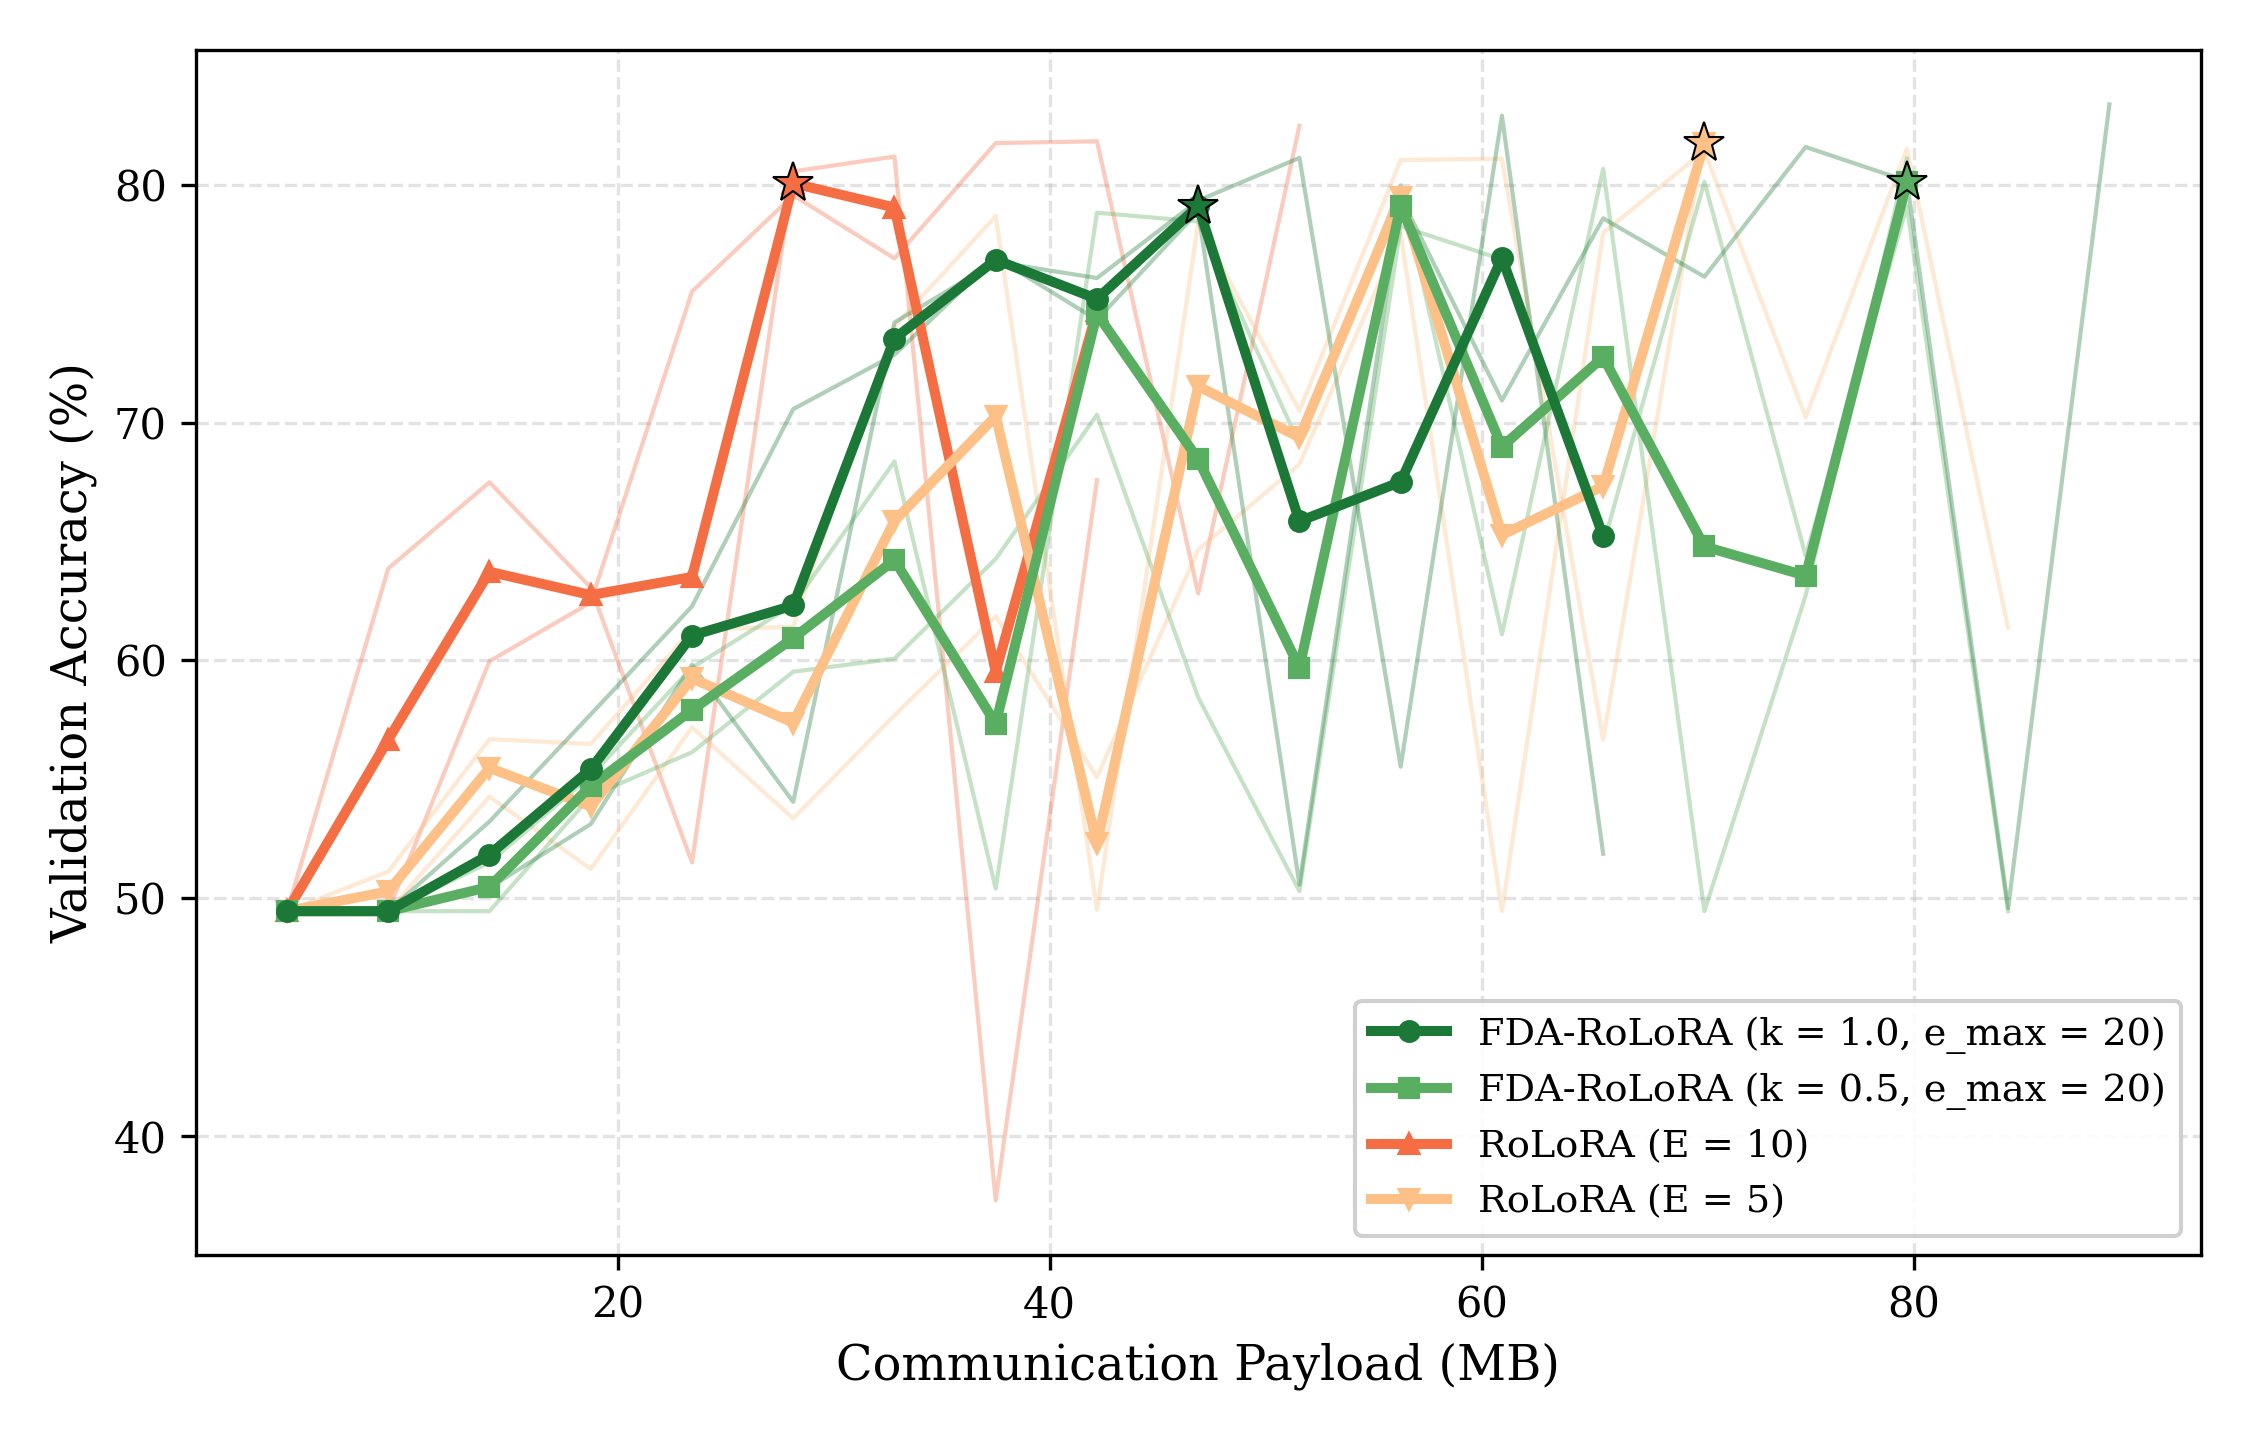
\includegraphics[width=\textwidth,height=4.9cm,keepaspectratio]{figures/telemetry/05_QNLI_C20_R50_LR0.1_4_accuracy_vs_cost.png}
            \vspace{2pt}
            \par{\footnotesize \textbf{(b)} Accuracy vs. Communication (MB)}
        \end{minipage}

        \vspace{0.6em}
        \begin{minipage}[b]{0.485\textwidth}
            \centering
            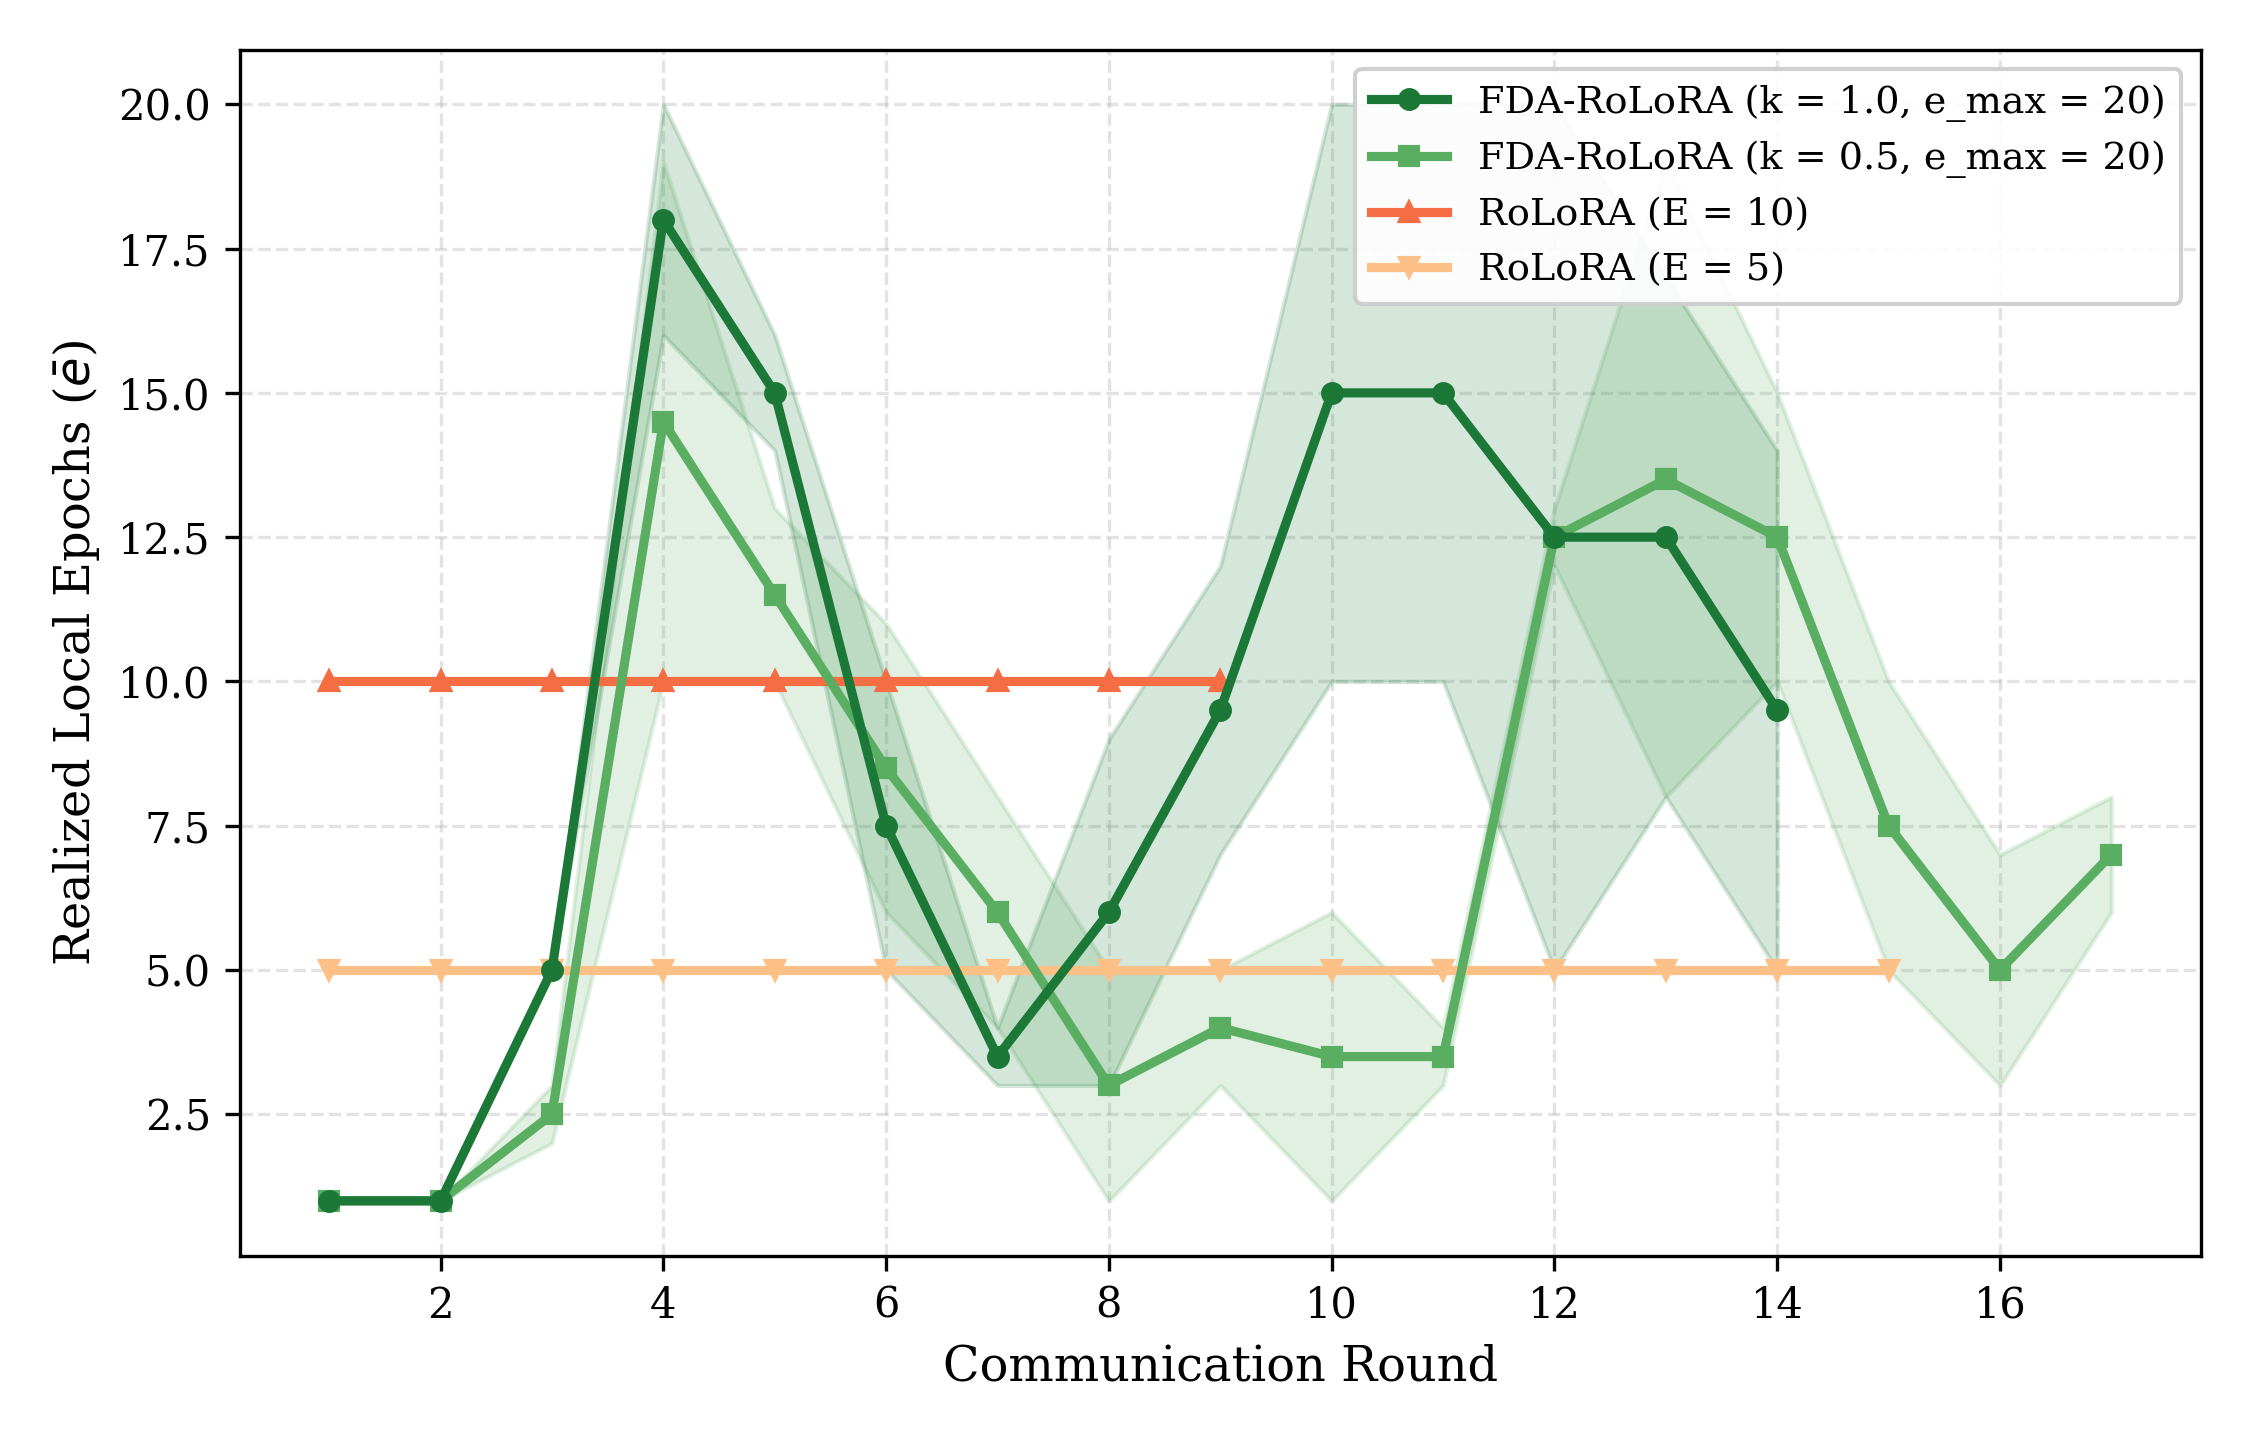
\includegraphics[width=\textwidth,height=4.9cm,keepaspectratio]{figures/telemetry/05_QNLI_C20_R50_LR0.1_2_allocated_epochs.png}
            \vspace{2pt}
            \par{\footnotesize \textbf{(c)} Dynamic Local Epochs ($\bar{e}$)}
        \end{minipage}\hfill
        \begin{minipage}[b]{0.485\textwidth}
            \centering
            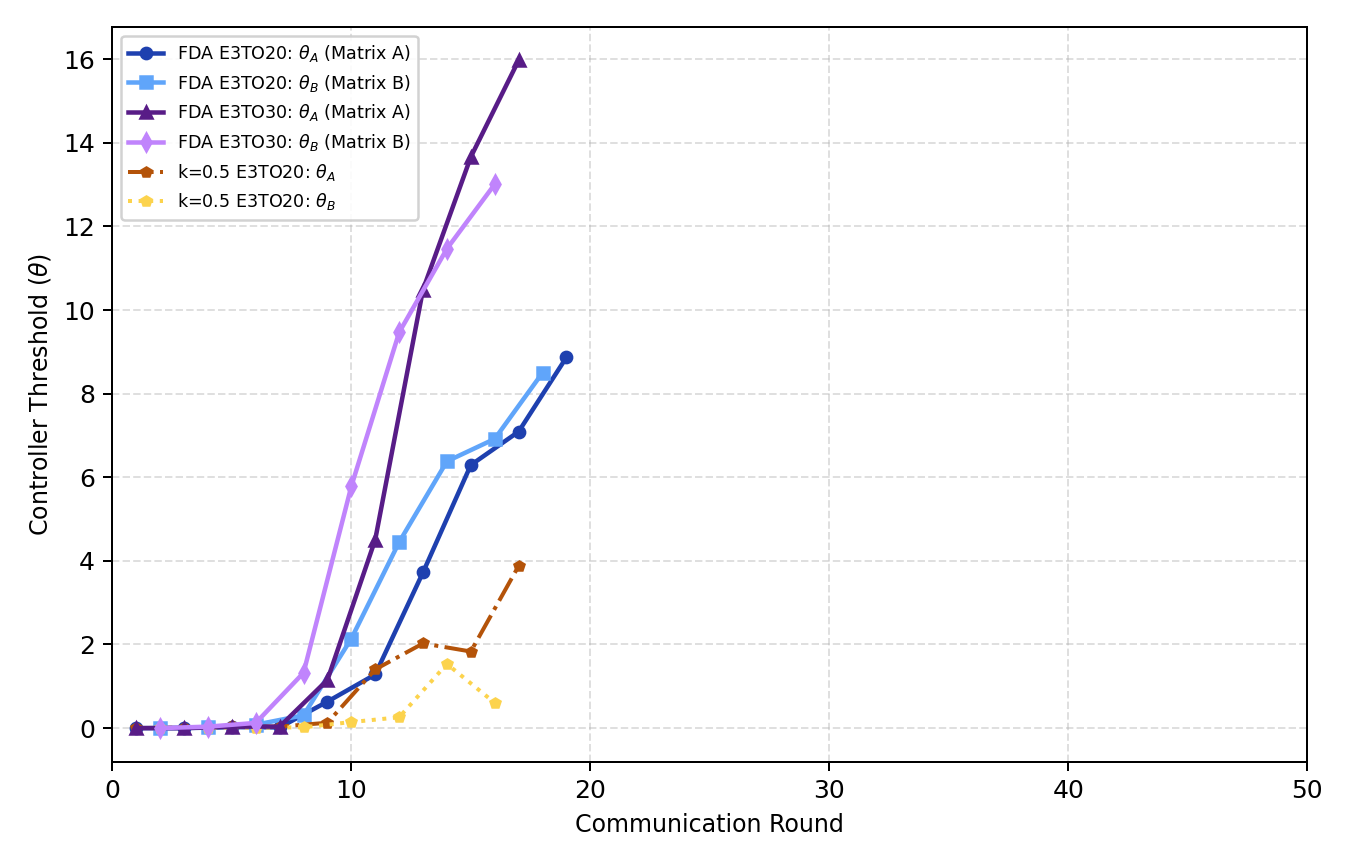
\includegraphics[width=\textwidth,height=4.9cm,keepaspectratio]{figures/telemetry/05_QNLI_C20_R50_LR0.1_5_fda_threshold.png}
            \vspace{2pt}
            \par{\footnotesize \textbf{(d)} Factor Thresholds ($\theta_A, \theta_B$)}
        \end{minipage}

        \vspace{0.6em}
        \begin{minipage}[b]{0.485\textwidth}
            \centering
            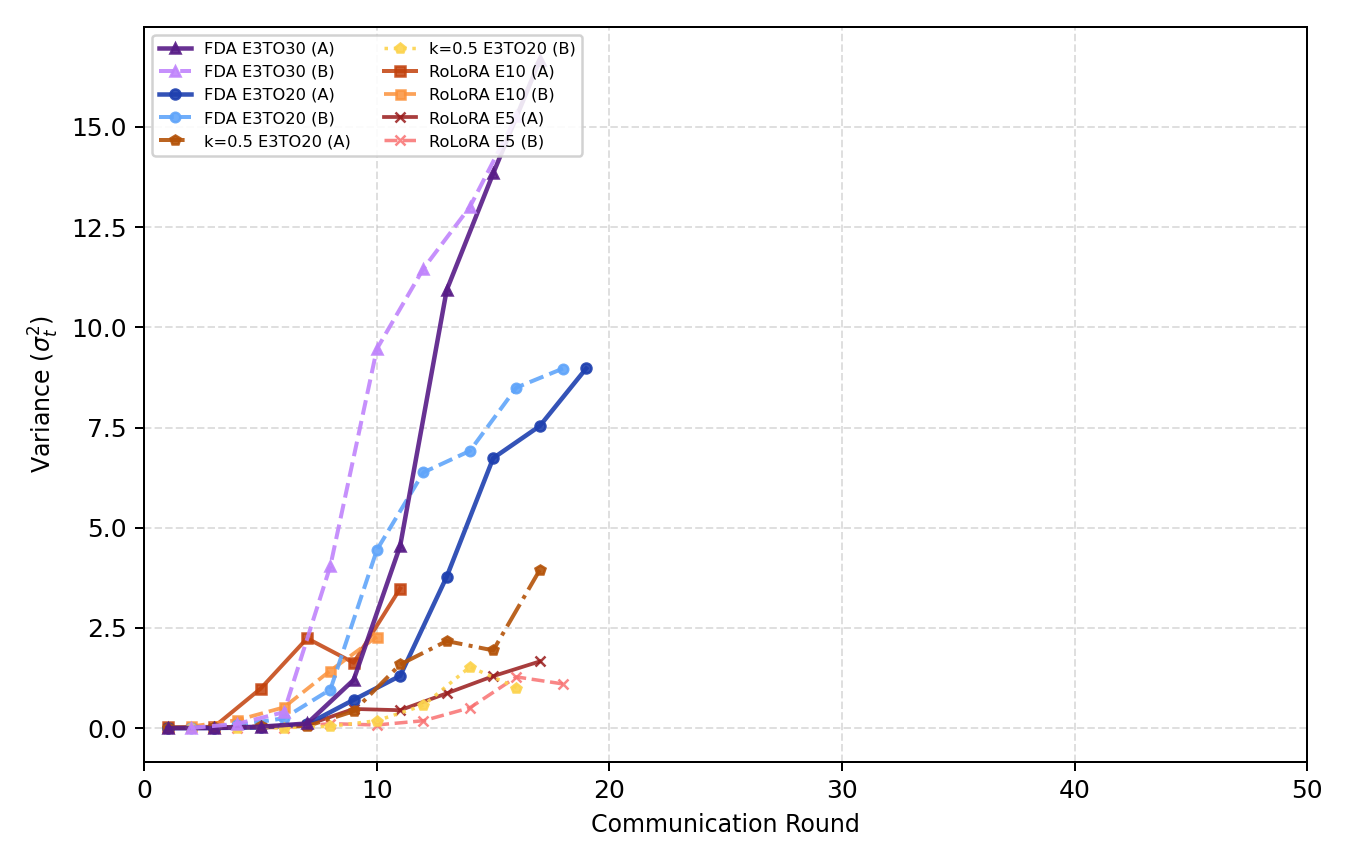
\includegraphics[width=\textwidth,height=4.9cm,keepaspectratio]{figures/telemetry/05_QNLI_C20_R50_LR0.1_3_client_variance.png}
            \vspace{2pt}
            \par{\footnotesize \textbf{(e)} Subspace Coordinate Variance}
        \end{minipage}\hfill
        \begin{minipage}[b]{0.485\textwidth}
            \centering
            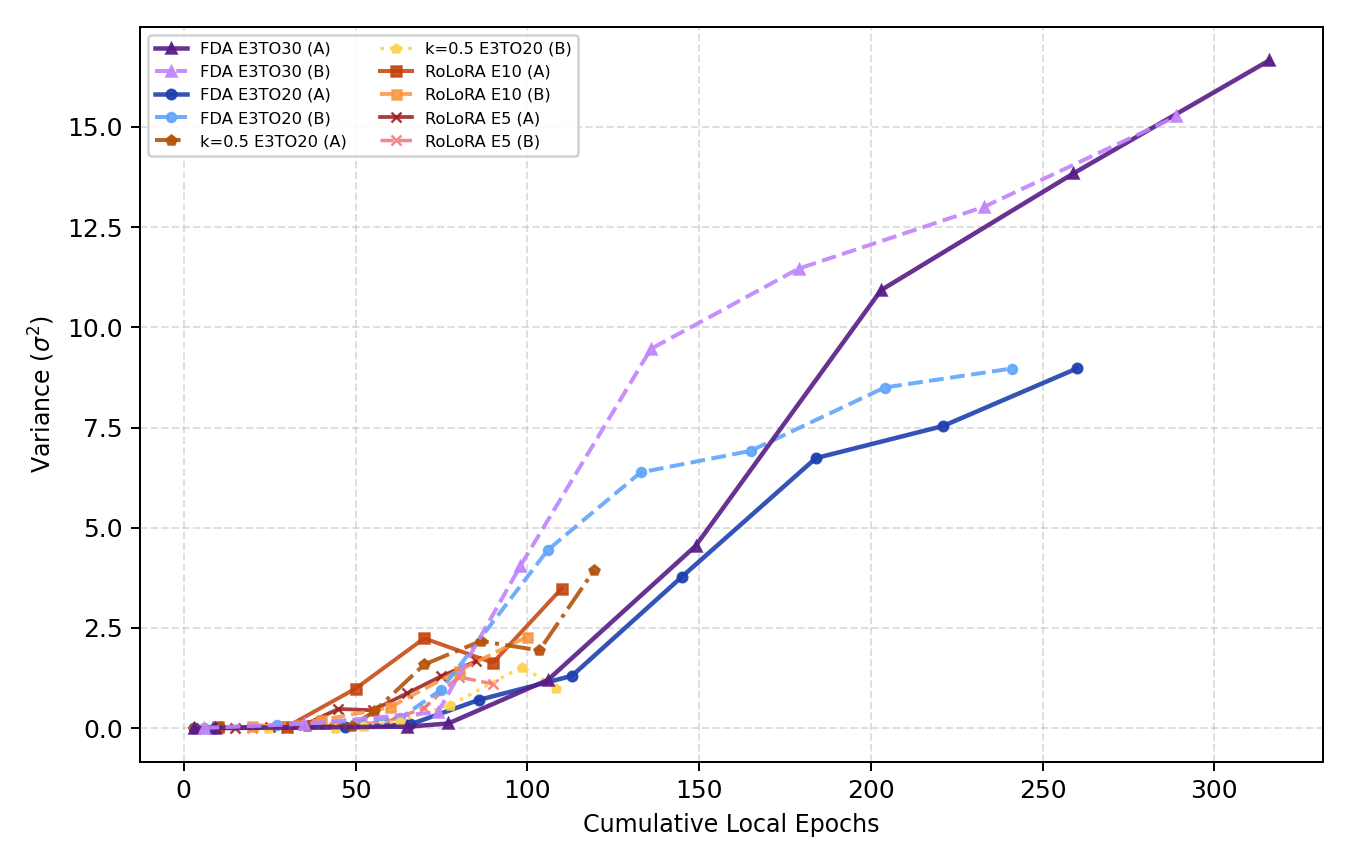
\includegraphics[width=\textwidth,height=4.9cm,keepaspectratio]{figures/telemetry/05_QNLI_C20_R50_LR0.1_6_variance_vs_epoch.png}
            \vspace{2pt}
            \par{\footnotesize \textbf{(f)} Variance vs.\ Cumulative Local Epochs}
        \end{minipage}

        \vspace{0.6em}
        \caption{Multi-panel optimization telemetry on QNLI ($C=20, R_{\max}=50, \eta_c=0.1, \alpha=1000.0$) comparing FDA-RoLoRA against static RoLoRA baselines under homogeneous consensus.}
        \label{fig:telemetry_qnli_c20_iid}
    \end{minipage}%
    }
\end{figure}

\begin{figure}[p]
    \centering
    \makebox[\textwidth][c]{%
    \begin{minipage}{1.06\textwidth}
        \begin{minipage}[b]{0.485\textwidth}
            \centering
            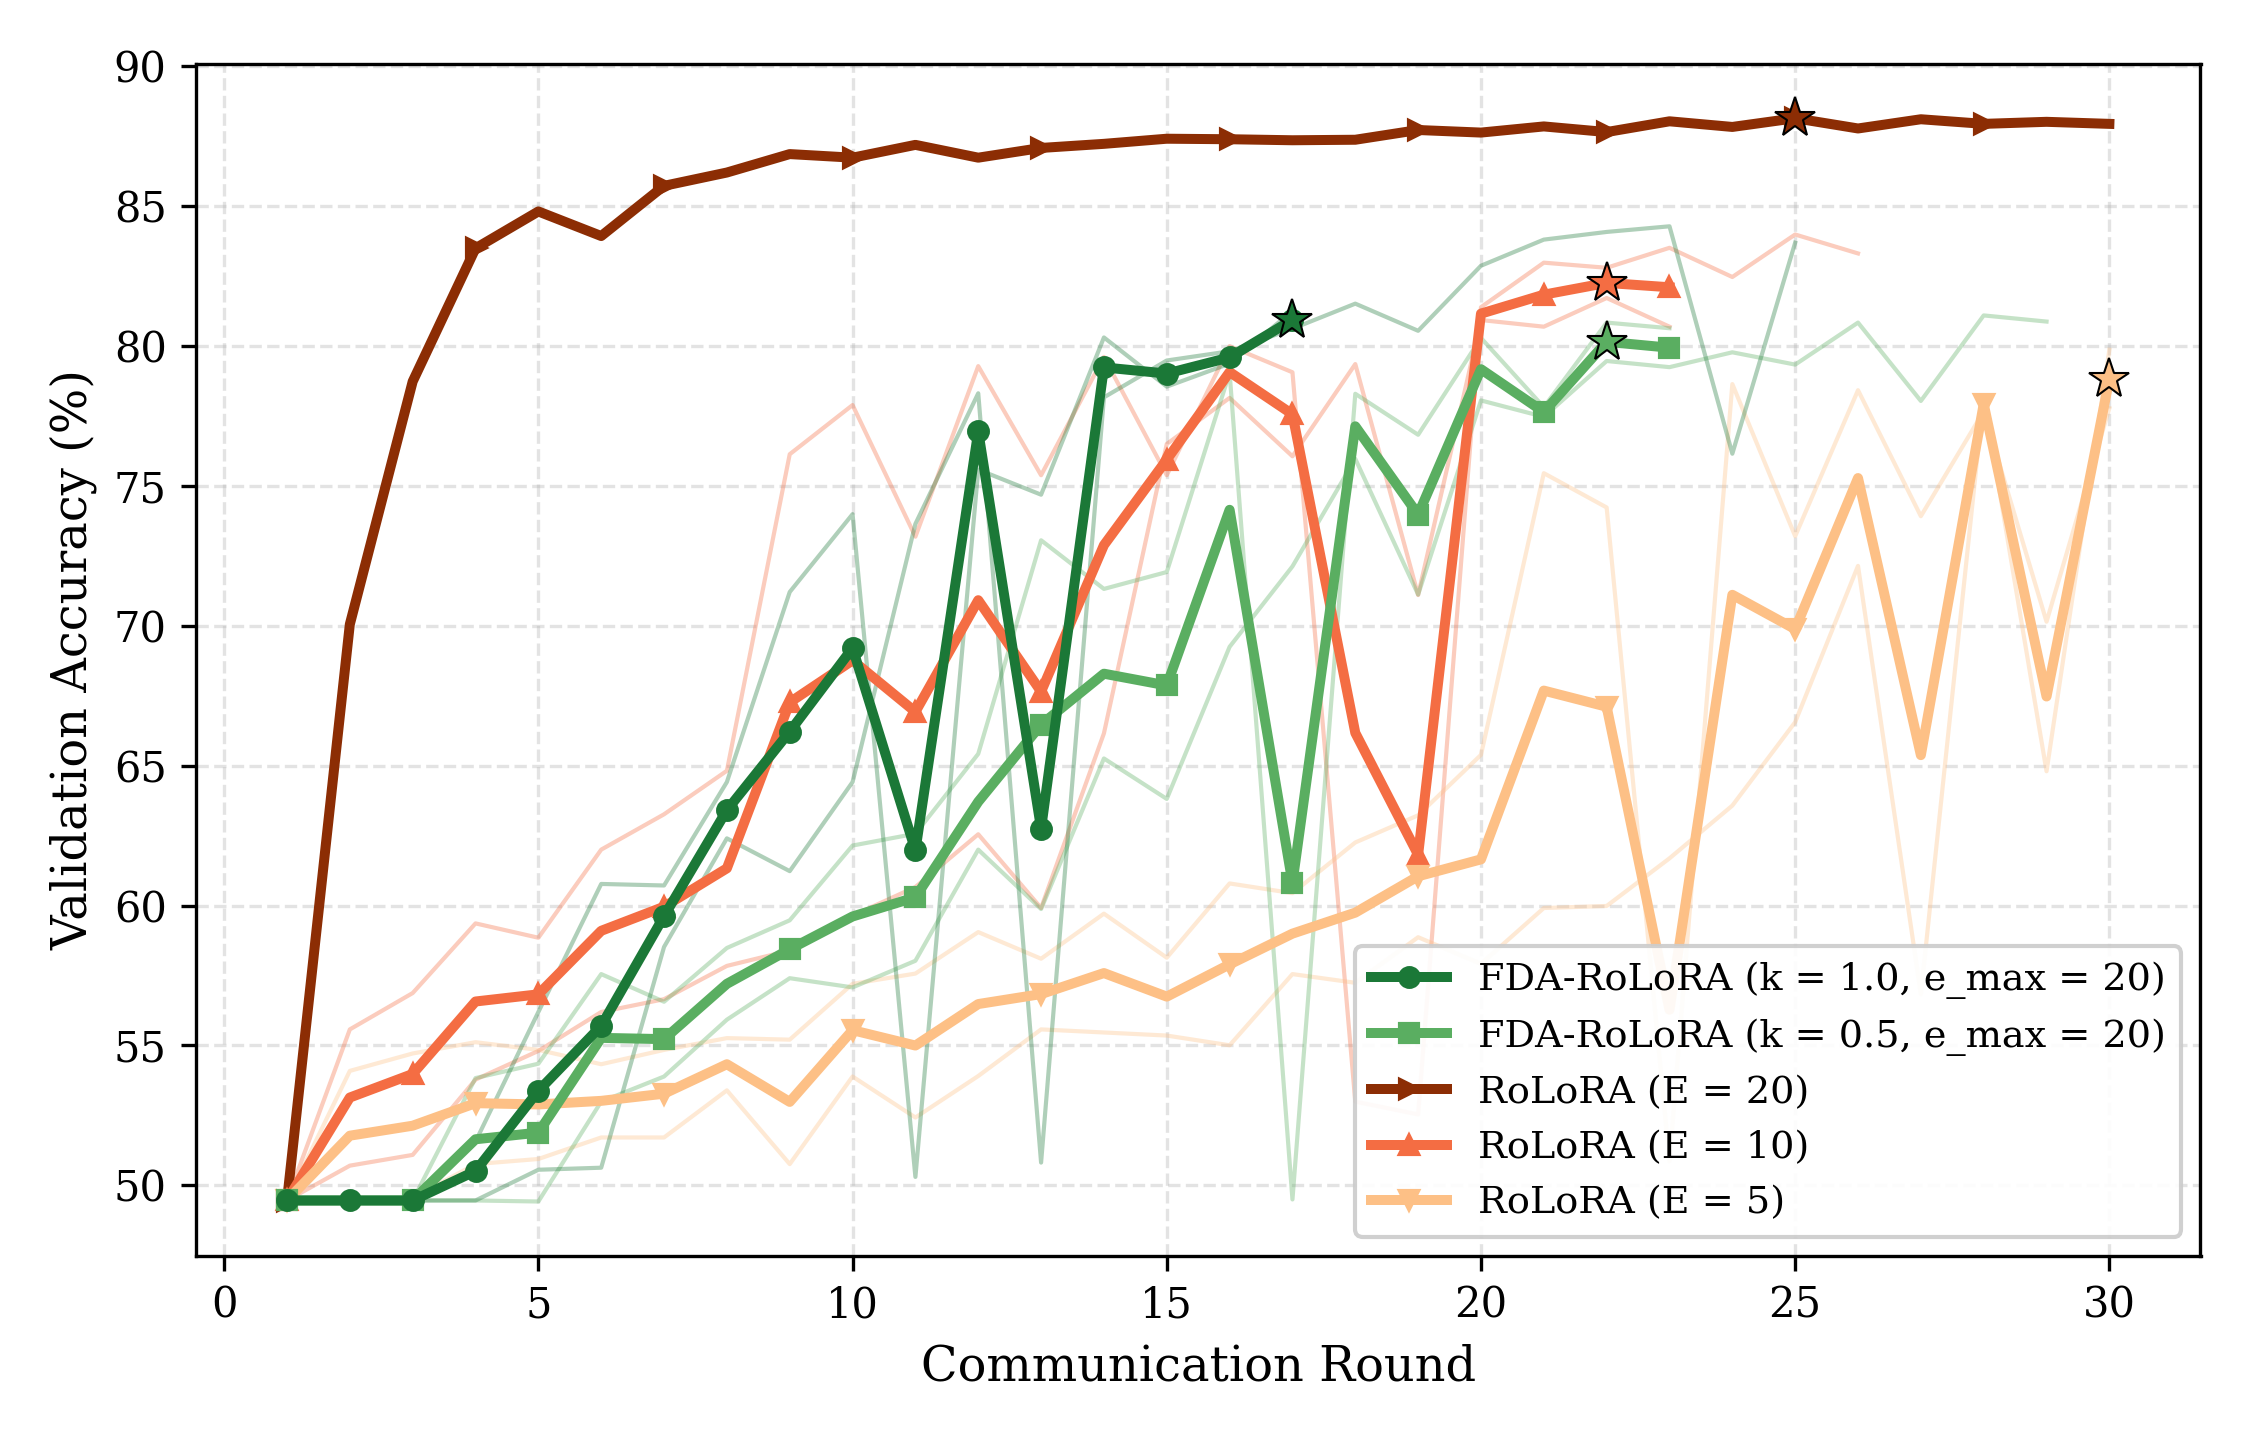
\includegraphics[width=\textwidth,height=4.9cm,keepaspectratio]{figures/telemetry/07_QNLI_C50_R30_LR0.1_1_accuracy.png}
            \vspace{2pt}
            \par{\footnotesize \textbf{(a)} Validation Accuracy}
        \end{minipage}\hfill
        \begin{minipage}[b]{0.485\textwidth}
            \centering
            \includegraphics[width=\textwidth,height=4.9cm,keepaspectratio]{figures/telemetry/07_QNLI_C50_R30_LR0.1_4_accuracy_vs_cost.png}
            \vspace{2pt}
            \par{\footnotesize \textbf{(b)} Accuracy vs. Communication (MB)}
        \end{minipage}

        \vspace{0.6em}
        \begin{minipage}[b]{0.485\textwidth}
            \centering
            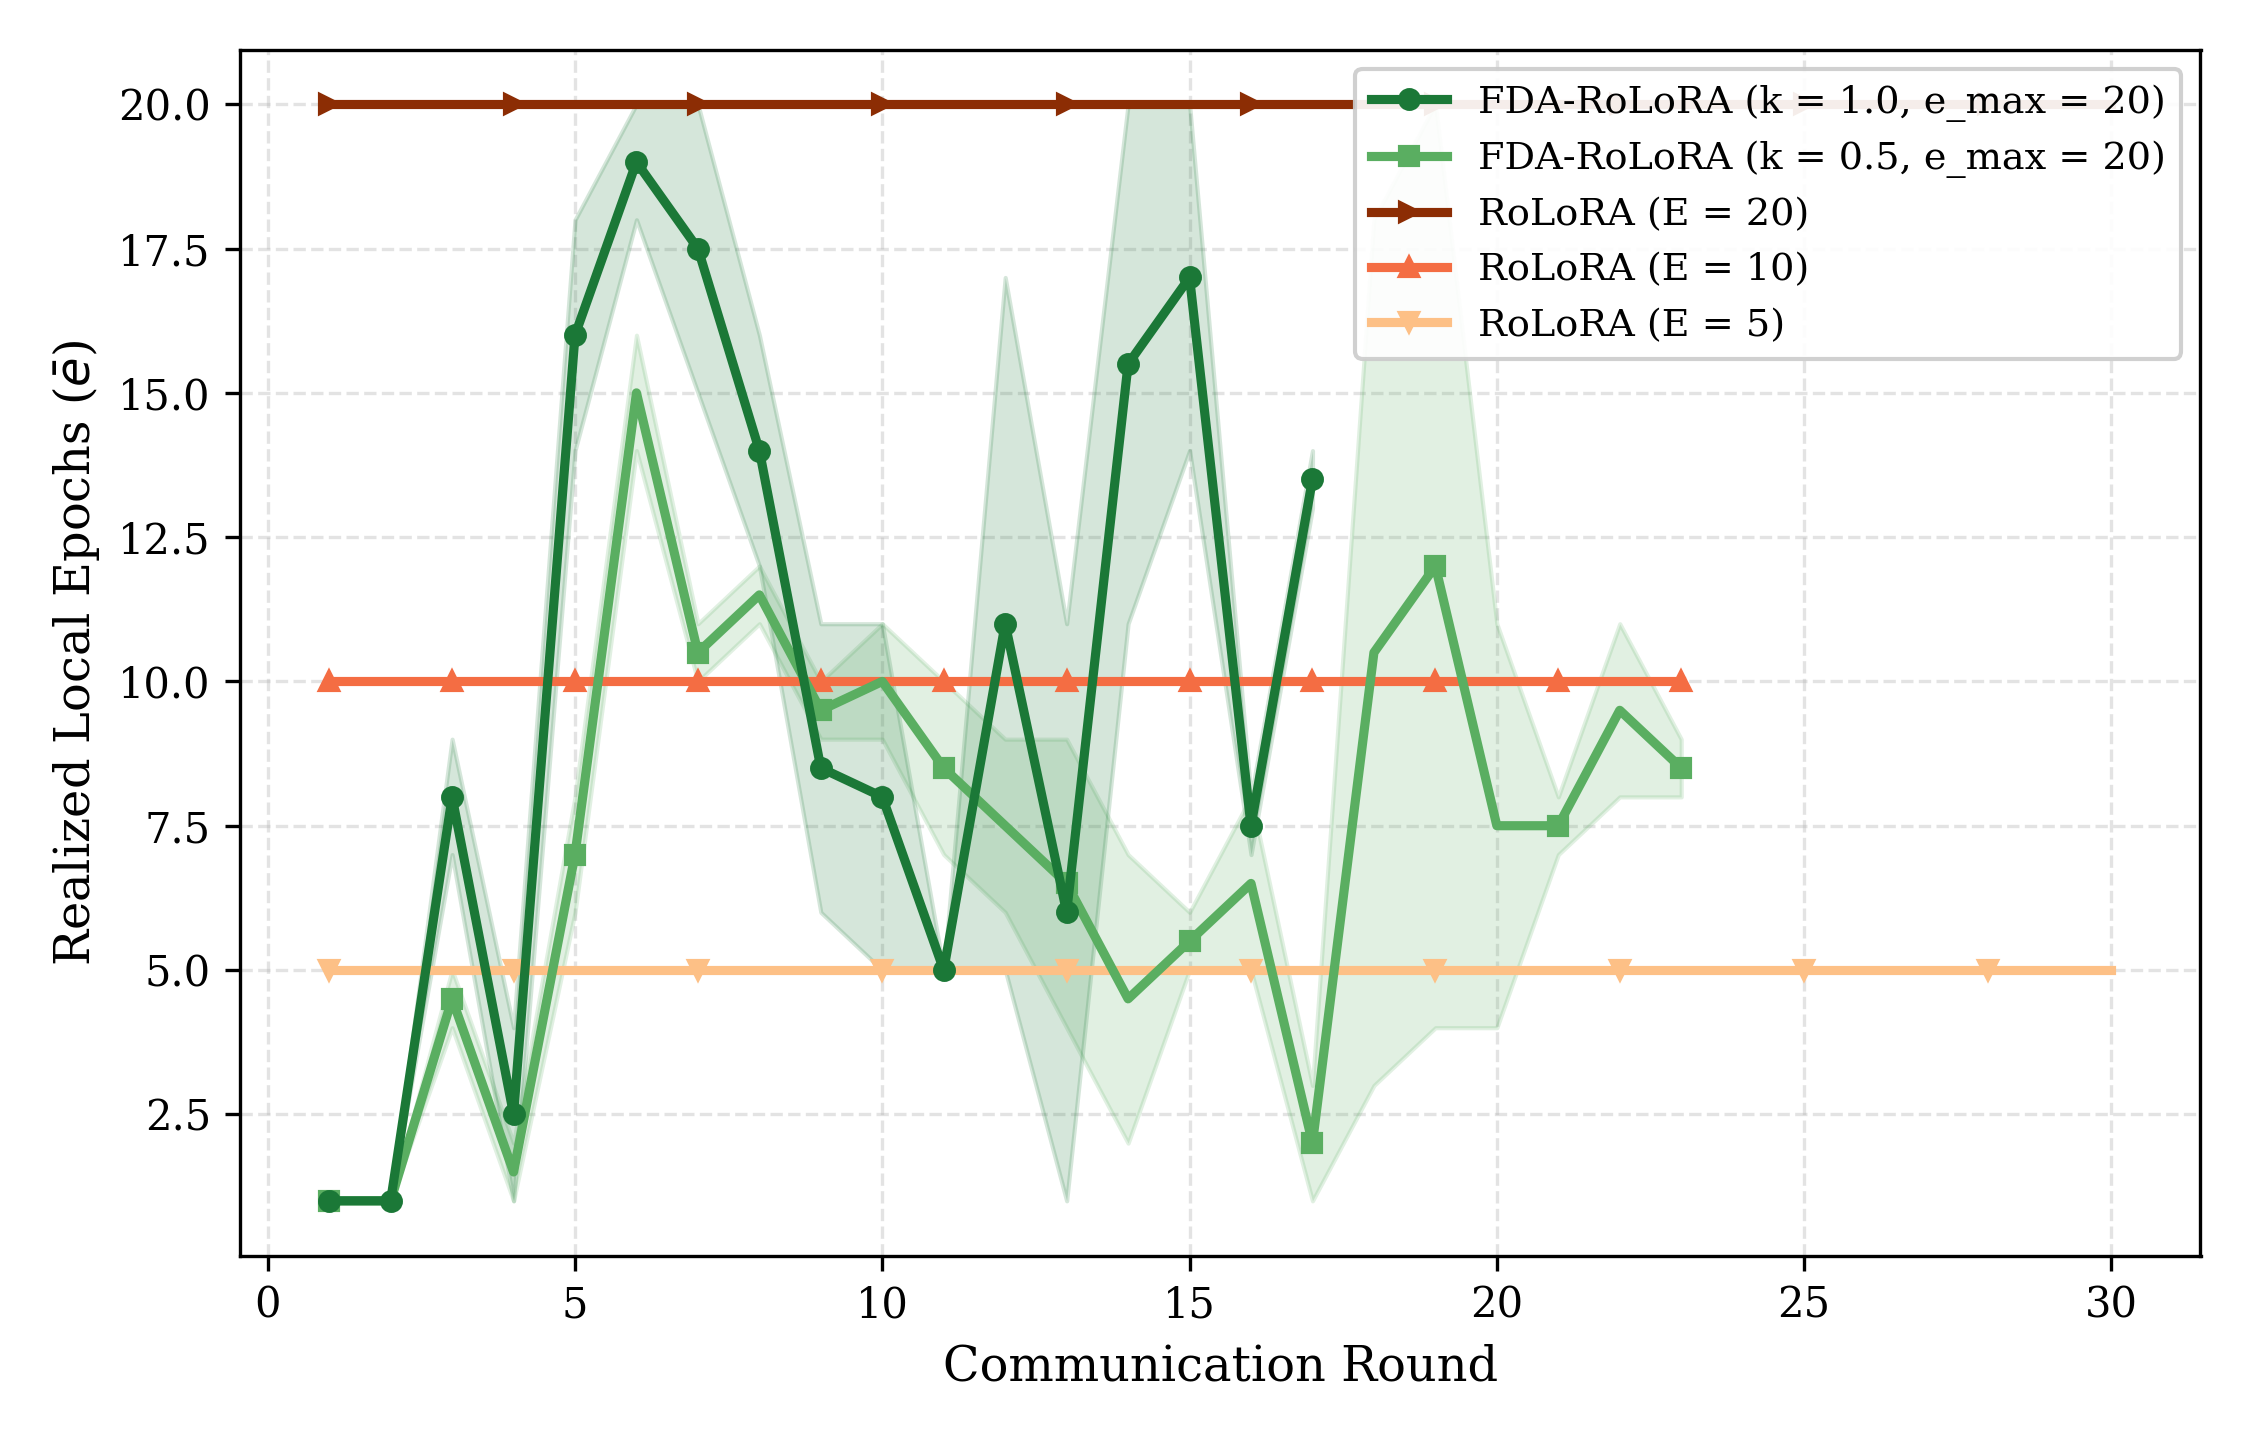
\includegraphics[width=\textwidth,height=4.9cm,keepaspectratio]{figures/telemetry/07_QNLI_C50_R30_LR0.1_2_allocated_epochs.png}
            \vspace{2pt}
            \par{\footnotesize \textbf{(c)} Dynamic Local Epochs ($\bar{e}$)}
        \end{minipage}\hfill
        \begin{minipage}[b]{0.485\textwidth}
            \centering
            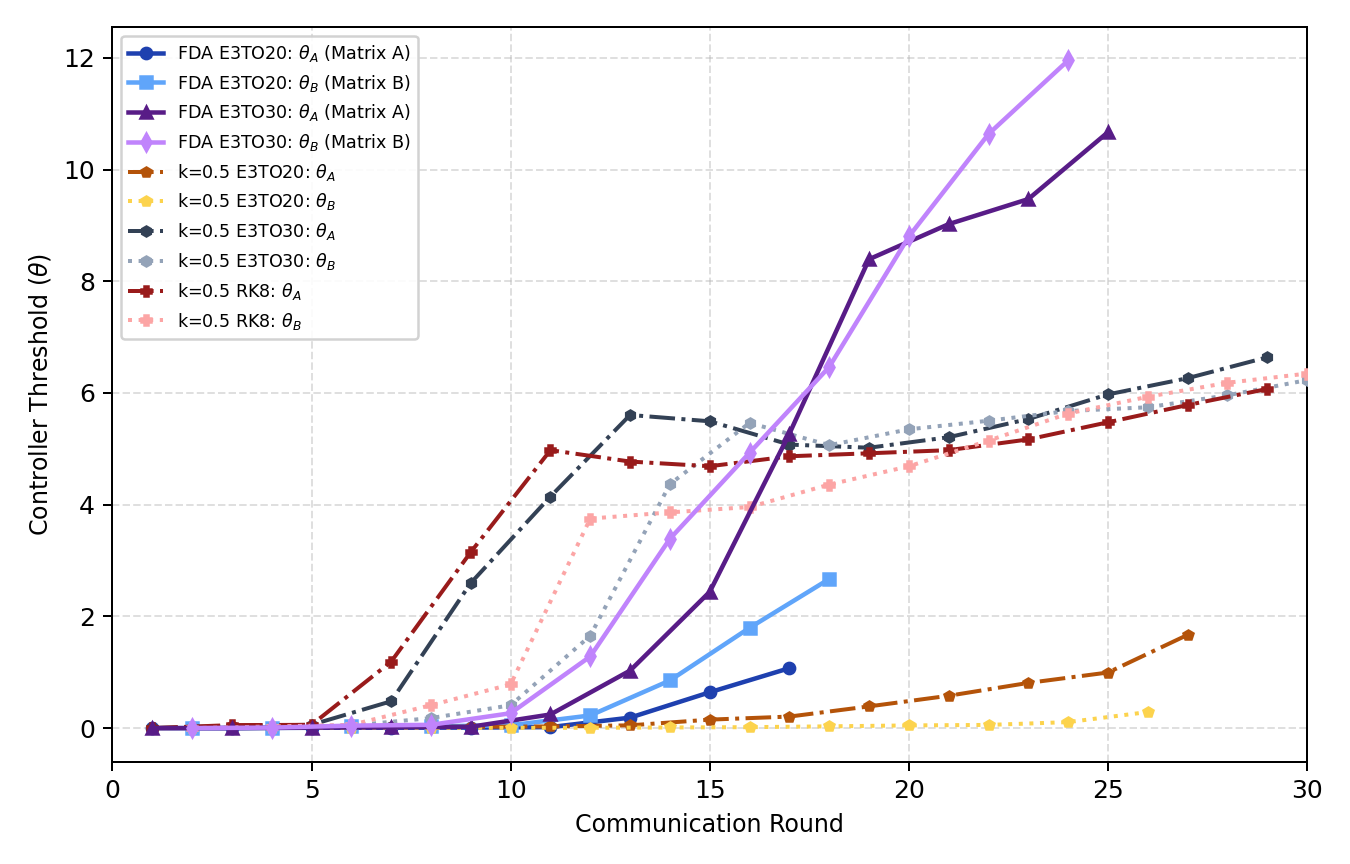
\includegraphics[width=\textwidth,height=4.9cm,keepaspectratio]{figures/telemetry/07_QNLI_C50_R30_LR0.1_5_fda_threshold.png}
            \vspace{2pt}
            \par{\footnotesize \textbf{(d)} Factor Thresholds ($\theta_A, \theta_B$)}
        \end{minipage}

        \vspace{0.6em}
        \begin{minipage}[b]{0.485\textwidth}
            \centering
            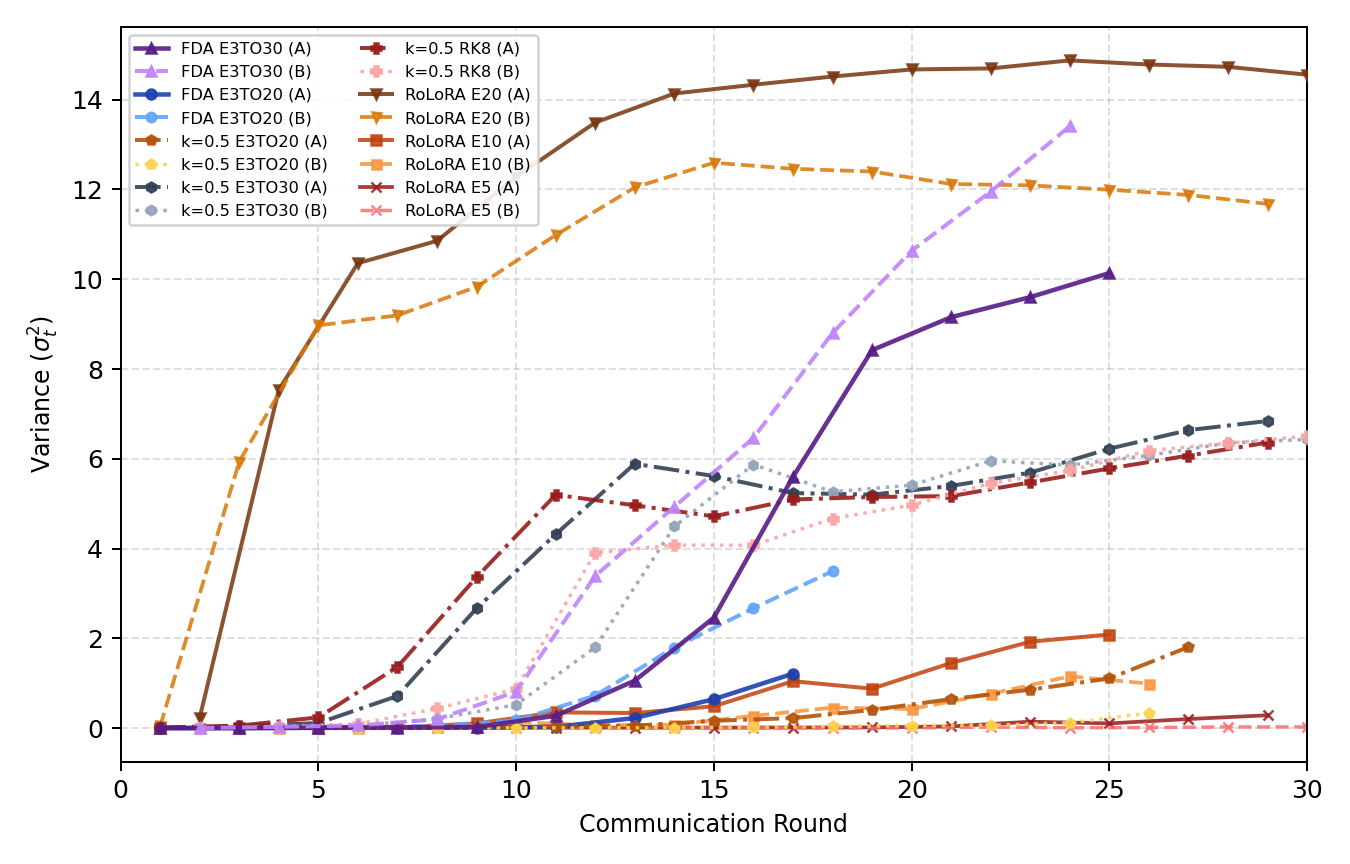
\includegraphics[width=\textwidth,height=4.9cm,keepaspectratio]{figures/telemetry/07_QNLI_C50_R30_LR0.1_3_client_variance.png}
            \vspace{2pt}
            \par{\footnotesize \textbf{(e)} Subspace Coordinate Variance}
        \end{minipage}\hfill
        \begin{minipage}[b]{0.485\textwidth}
            \centering
            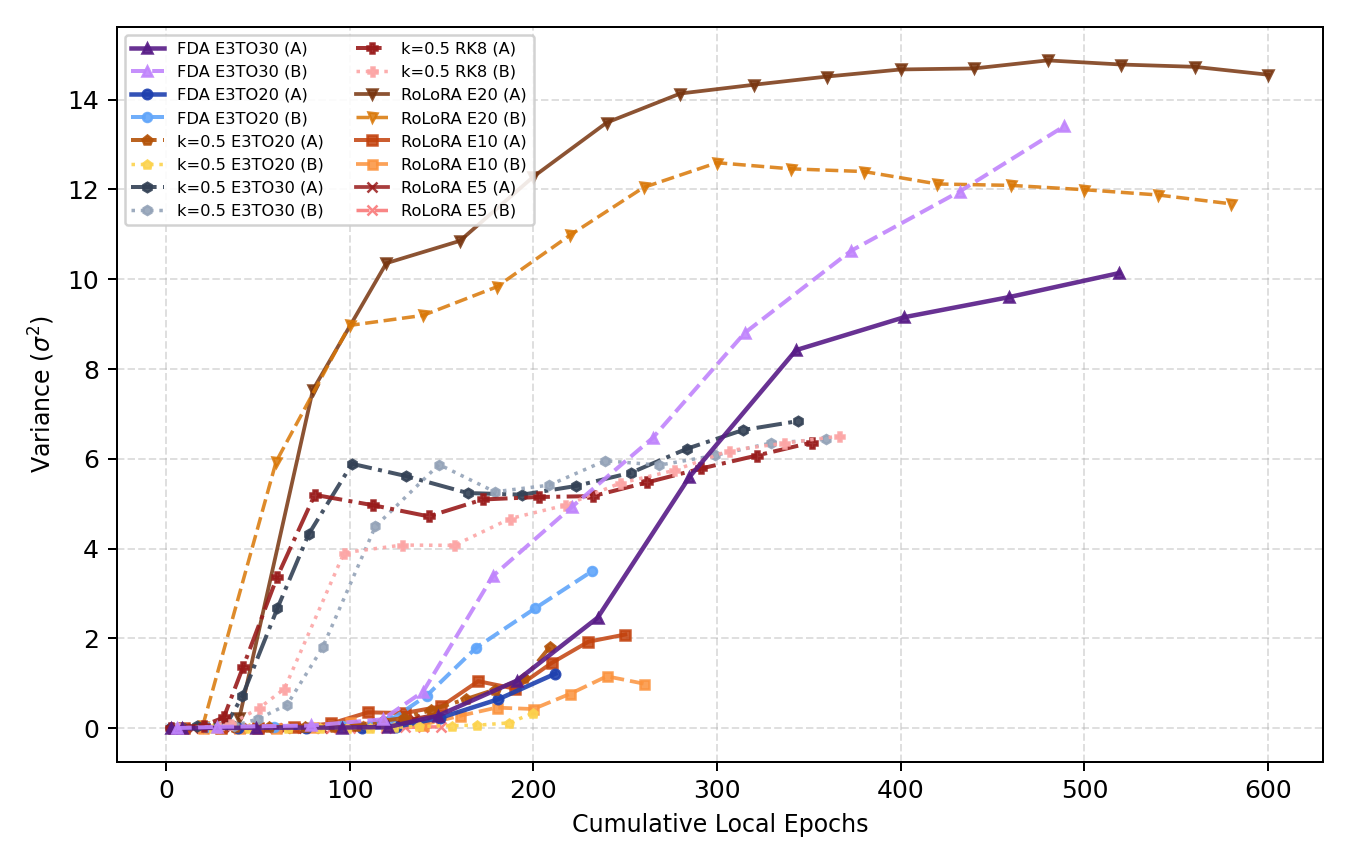
\includegraphics[width=\textwidth,height=4.9cm,keepaspectratio]{figures/telemetry/07_QNLI_C50_R30_LR0.1_6_variance_vs_epoch.png}
            \vspace{2pt}
            \par{\footnotesize \textbf{(f)} Variance vs.\ Cumulative Local Epochs}
        \end{minipage}

        \vspace{0.6em}
        \caption{Multi-panel optimization telemetry on QNLI ($C=50, R_{\max}=30, \eta_c=0.1, \alpha=1000.0$) under expanded cohort scale $C=50$.}
        \label{fig:telemetry_qnli_c50_iid}
    \end{minipage}%
    }
\end{figure}

\paragraph{QQP:}
Semantic paraphrase detection demonstrates the primary communication compression benefits of dynamic averaging. Figures~\ref{fig:telemetry_qqp_c20_iid} and \ref{fig:telemetry_qqp_c50_iid} illustrate QQP telemetry across all six metrics. On $C=20$ (Figure~\ref{fig:telemetry_qqp_c20_iid}), FDA-RoLoRA ($k=1.0$) attains $\mathbf{78.57\%}$ peak validation accuracy (Panel a), outperforming RoLoRA $E=10$ ($75.47\%$) by $\mathbf{+3.10\%}$ while shifting the cost Pareto curve leftward (Panel b). Realized local epochs (Panel c) average $\bar{e} = 10.69$ under $k=1.0$ (and $\bar{e} = 6.50$ under $k=0.5$). Factor threshold tracks (Panel d) adapt smoothly without volatility, while subspace coordinate variance (Panel e) is strictly bounded ($\bar{\nu} = 1.577$).

On $C=50$ (Figure~\ref{fig:telemetry_qqp_c50_iid}), static RoLoRA baselines require the full budget of $30.0$ rounds ($351.6\,\text{MB}$) without reaching early stopping. In contrast, FDA-RoLoRA ($k=1.0$) triggers early stopping after $14.0$ rounds ($164.1\,\text{MB}$) at a lower accuracy plateau (final $72.65\%$, peak $73.63\%$) than RoLoRA $E=10$ (final $75.43\%$, peak $78.79\%$). At the same round (round 14), RoLoRA $E=10$ had already reached $75.27\%$ and $75.90\%$ in the two seeds, and it matched FDA-RoLoRA's final accuracy by round 6--7. The earlier stop therefore reflects an earlier plateau, not a communication saving at equal accuracy. Guided by suppressed drift variance ($\bar{\nu} = 0.220$, Panel e), the controller safely executes $\bar{e} = 9.14$ epochs per round before synchronization.
\begin{figure}[p]
    \centering
    \makebox[\textwidth][c]{%
    \begin{minipage}{1.06\textwidth}
        \begin{minipage}[b]{0.485\textwidth}
            \centering
            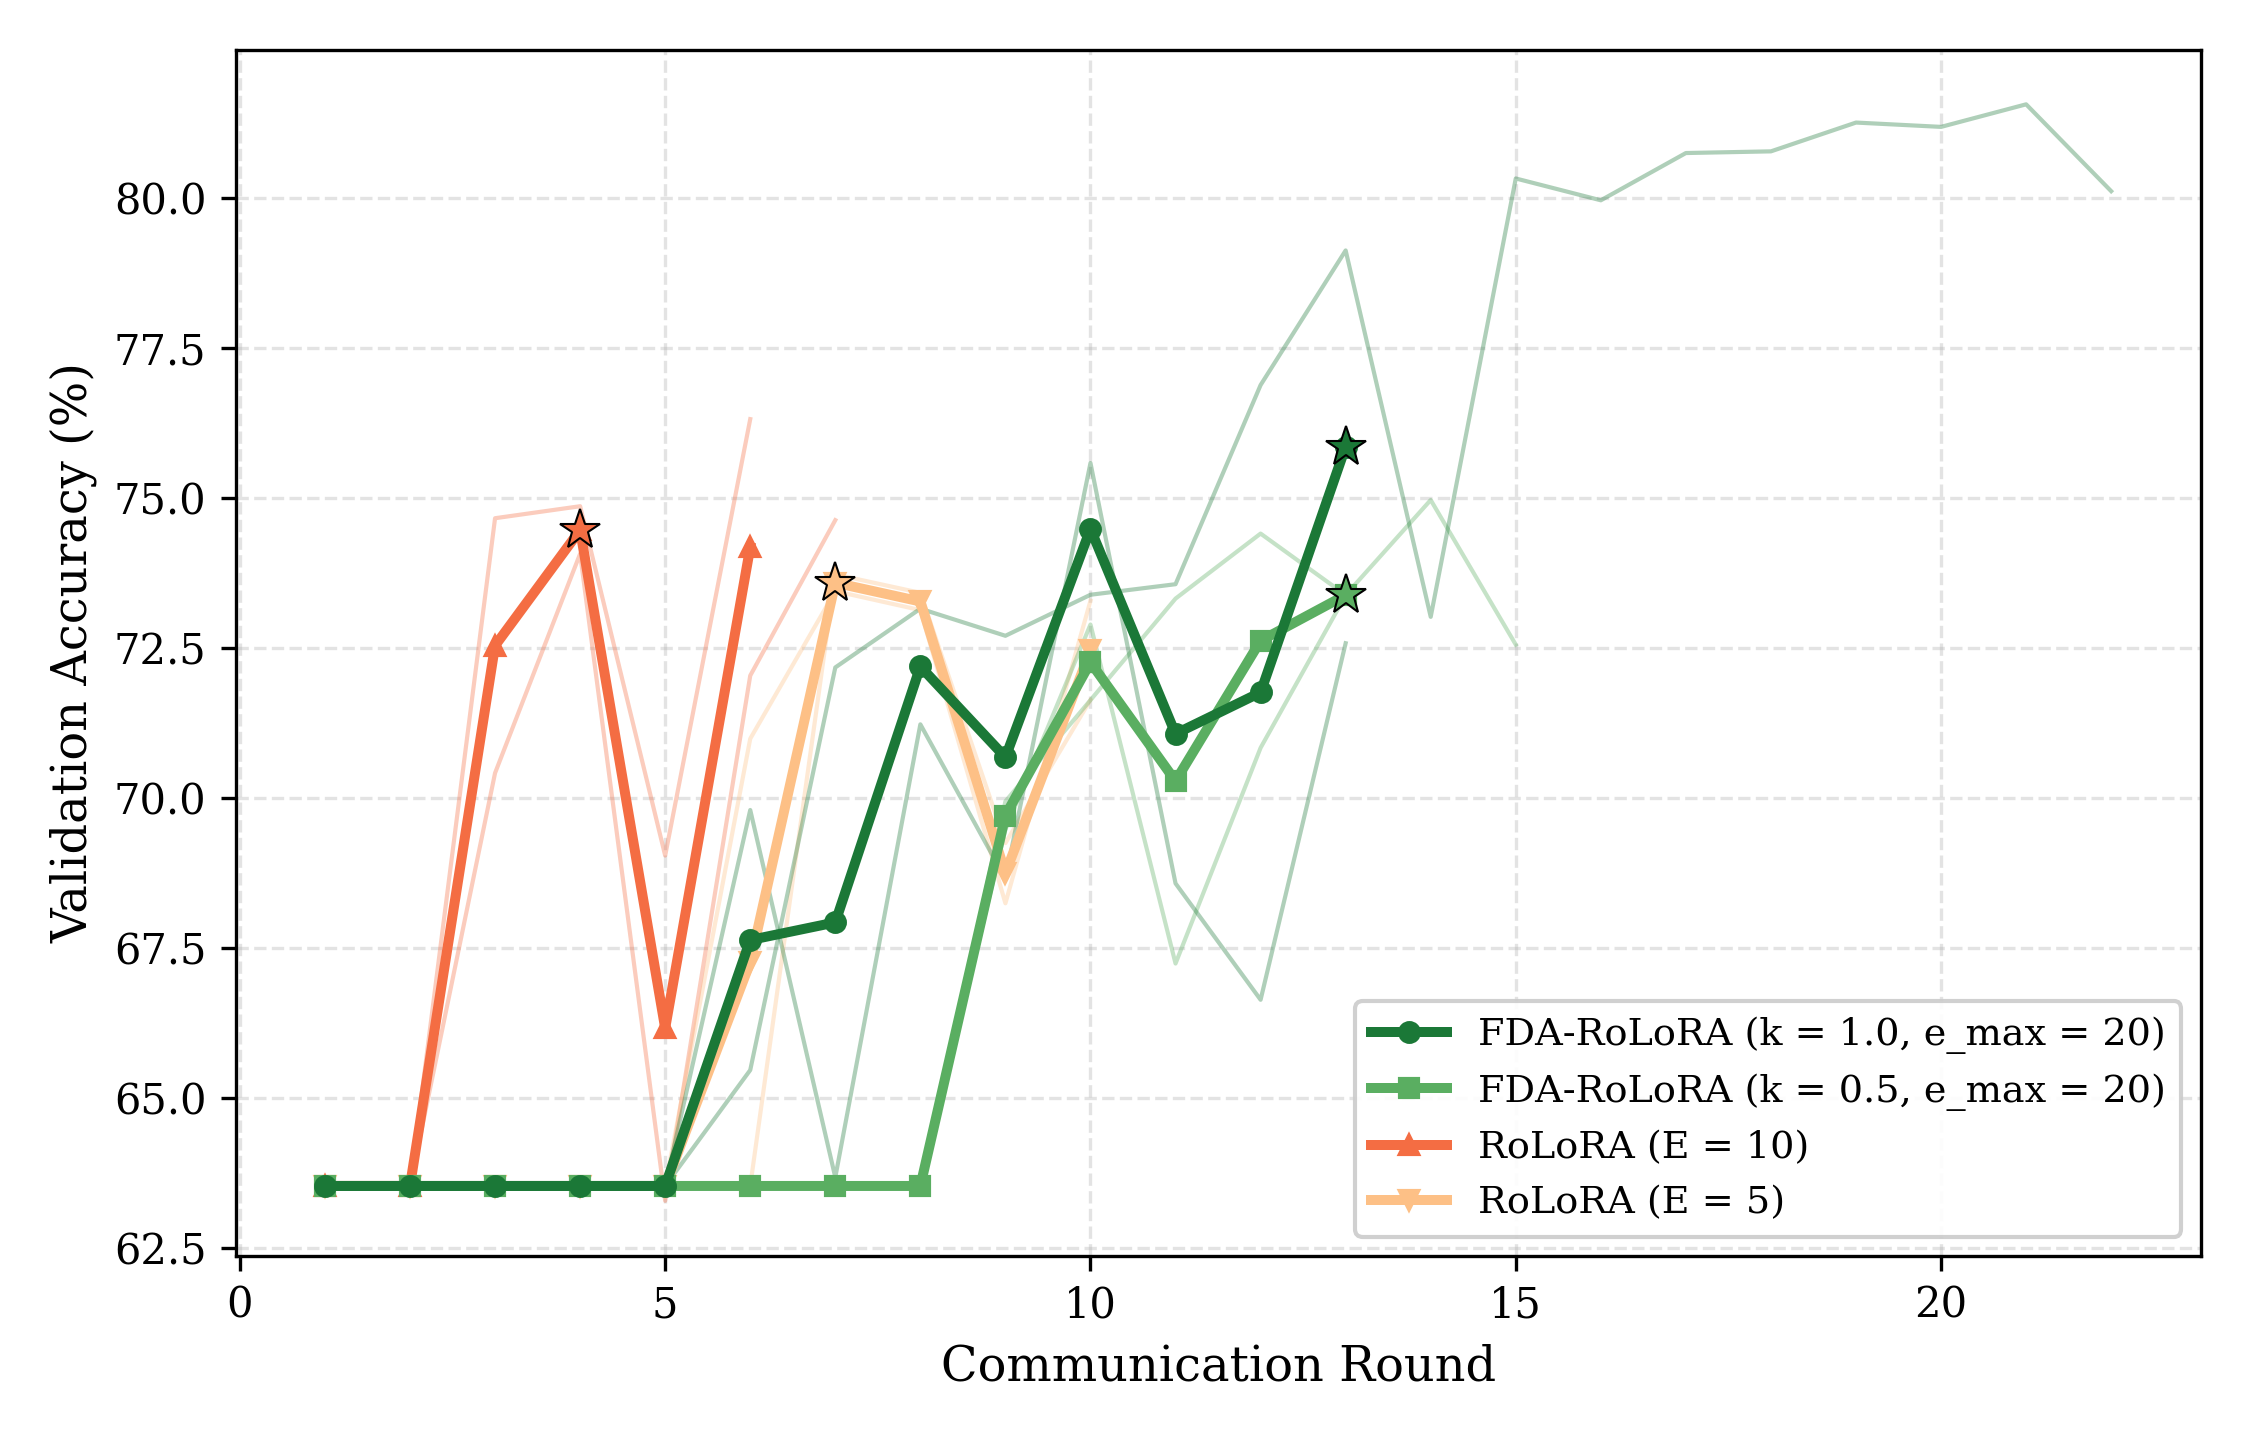
\includegraphics[width=\textwidth,height=4.9cm,keepaspectratio]{figures/telemetry/09_QQP_C20_R50_LR0.1_1_accuracy.png}
            \vspace{2pt}
            \par{\footnotesize \textbf{(a)} Validation Accuracy}
        \end{minipage}\hfill
        \begin{minipage}[b]{0.485\textwidth}
            \centering
            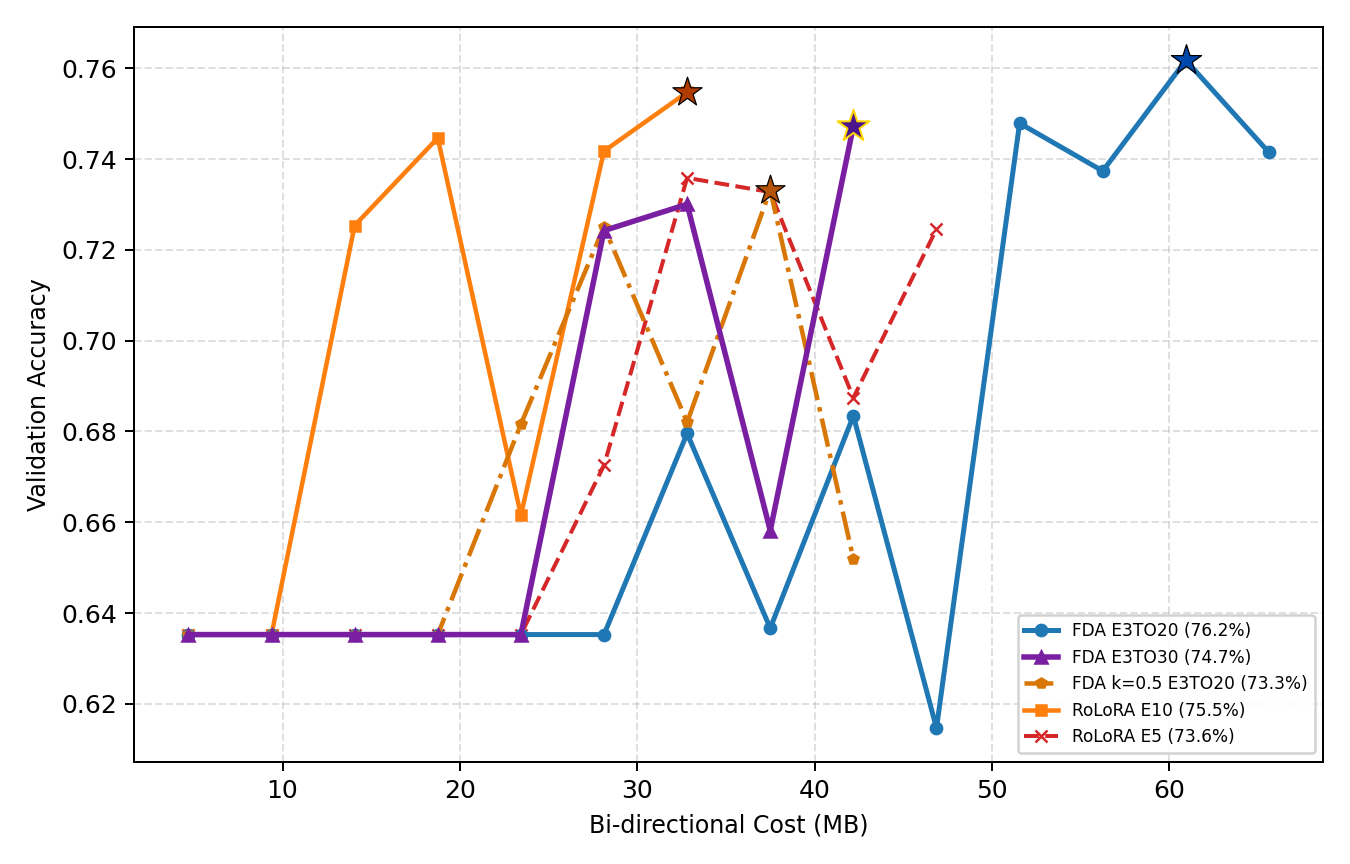
\includegraphics[width=\textwidth,height=4.9cm,keepaspectratio]{figures/telemetry/09_QQP_C20_R50_LR0.1_4_accuracy_vs_cost.png}
            \vspace{2pt}
            \par{\footnotesize \textbf{(b)} Accuracy vs. Communication (MB)}
        \end{minipage}

        \vspace{0.6em}
        \begin{minipage}[b]{0.485\textwidth}
            \centering
            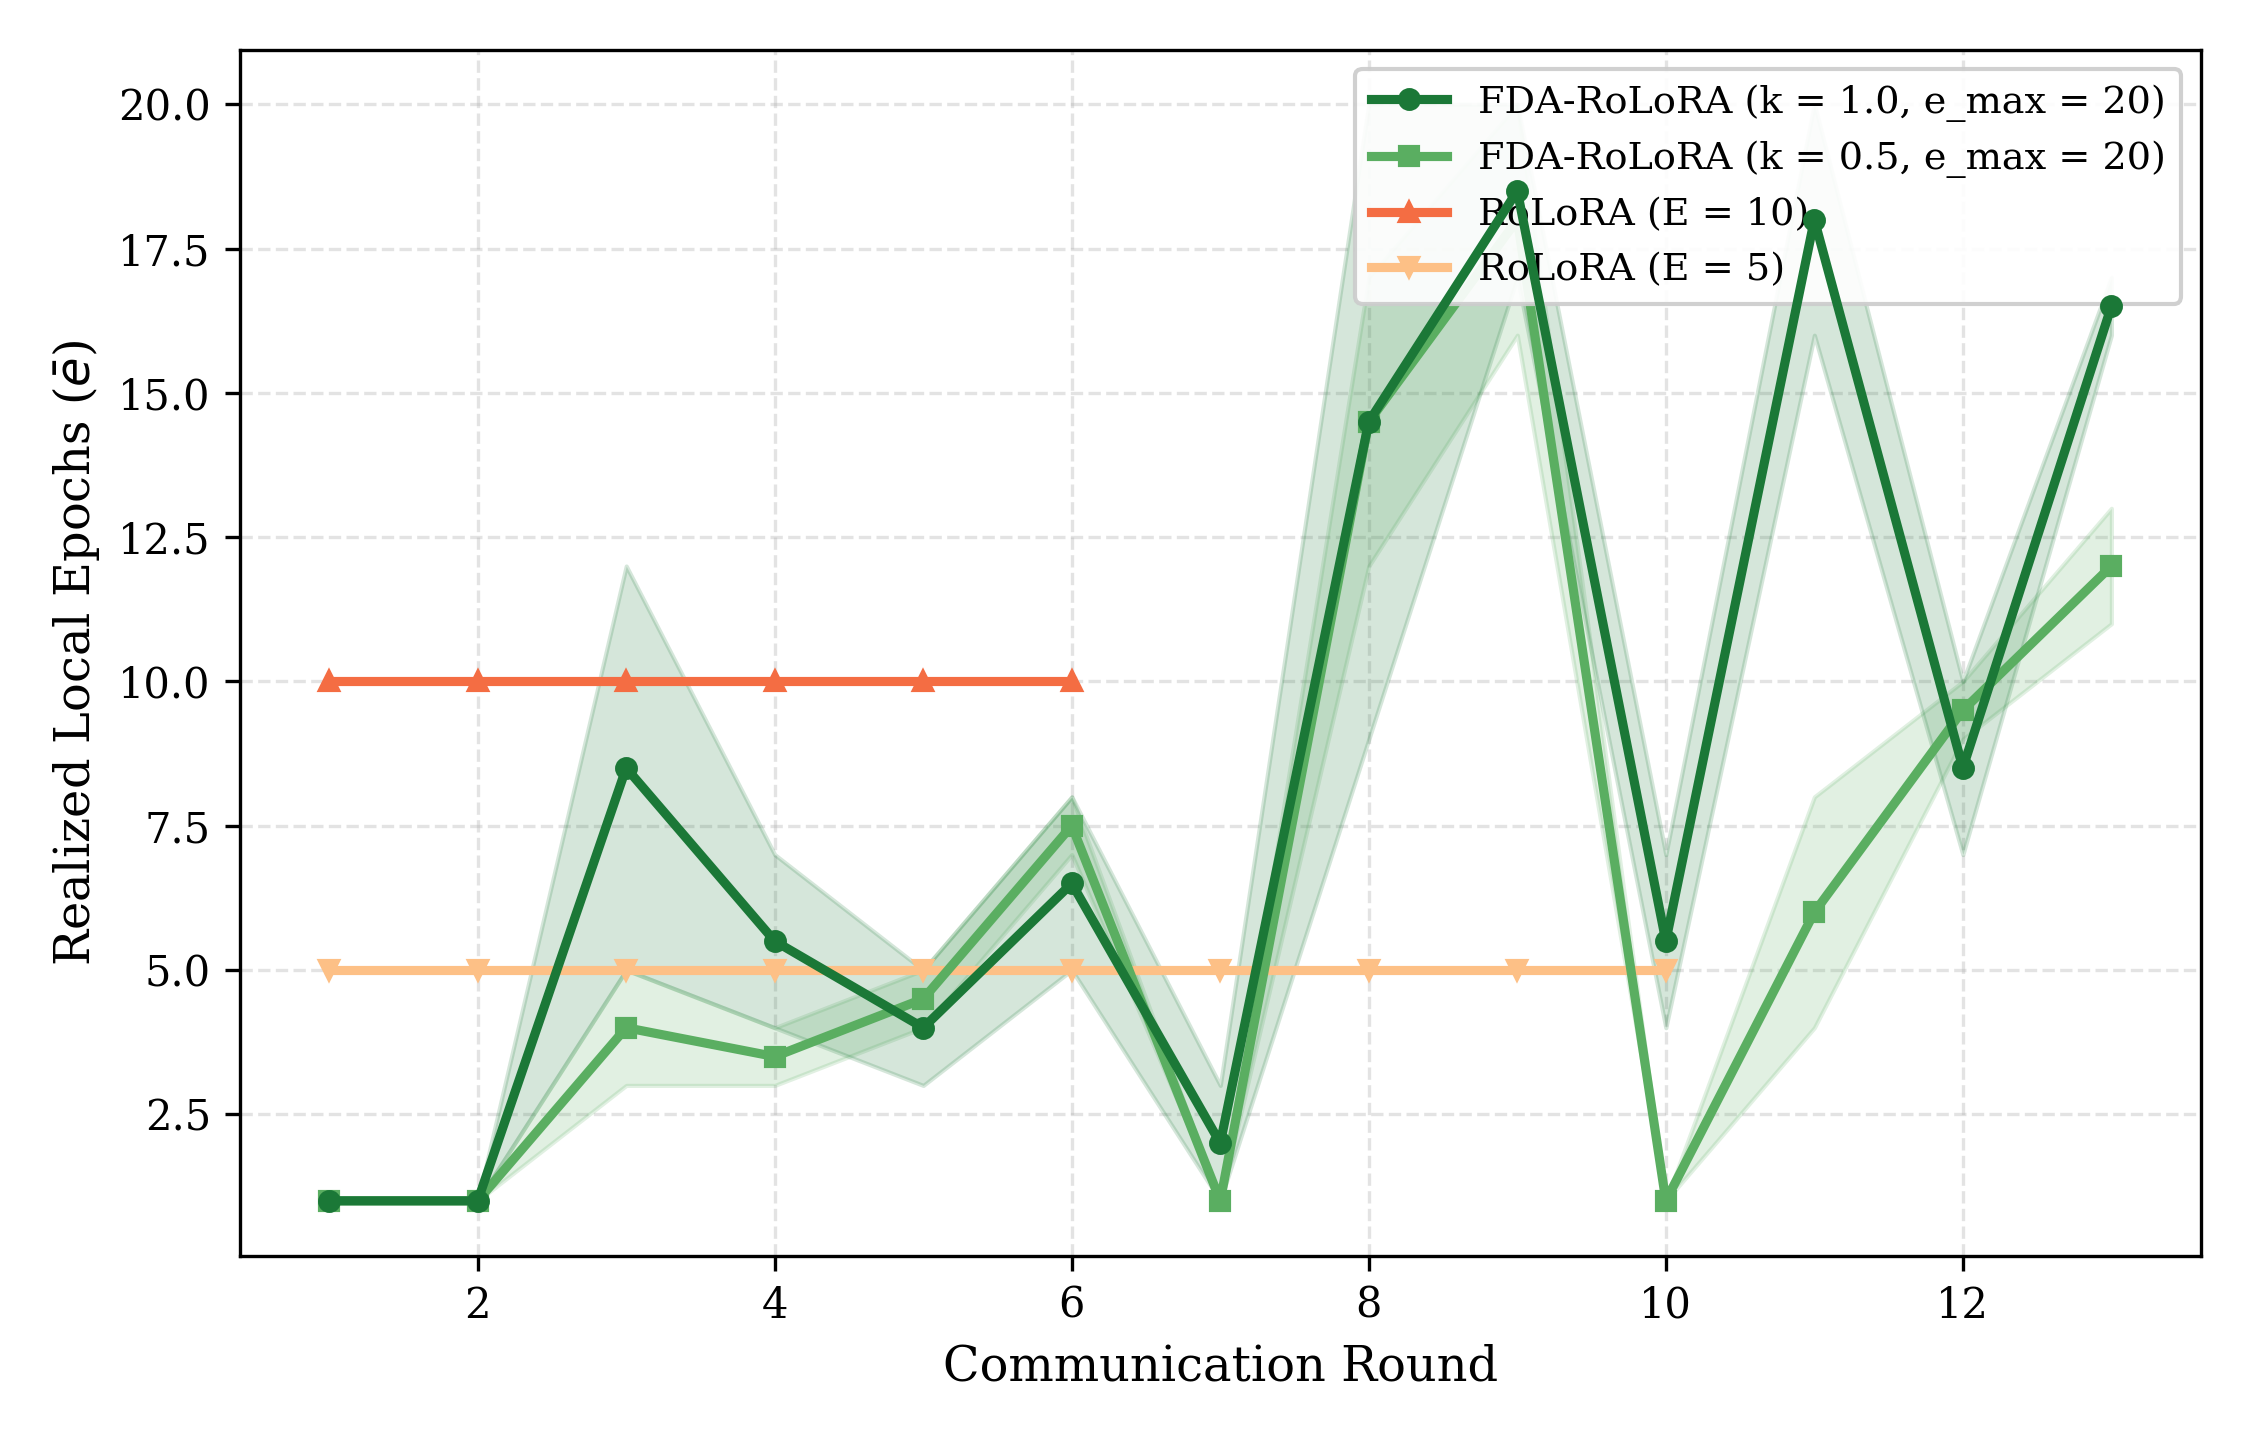
\includegraphics[width=\textwidth,height=4.9cm,keepaspectratio]{figures/telemetry/09_QQP_C20_R50_LR0.1_2_allocated_epochs.png}
            \vspace{2pt}
            \par{\footnotesize \textbf{(c)} Dynamic Local Epochs ($\bar{e}$)}
        \end{minipage}\hfill
        \begin{minipage}[b]{0.485\textwidth}
            \centering
            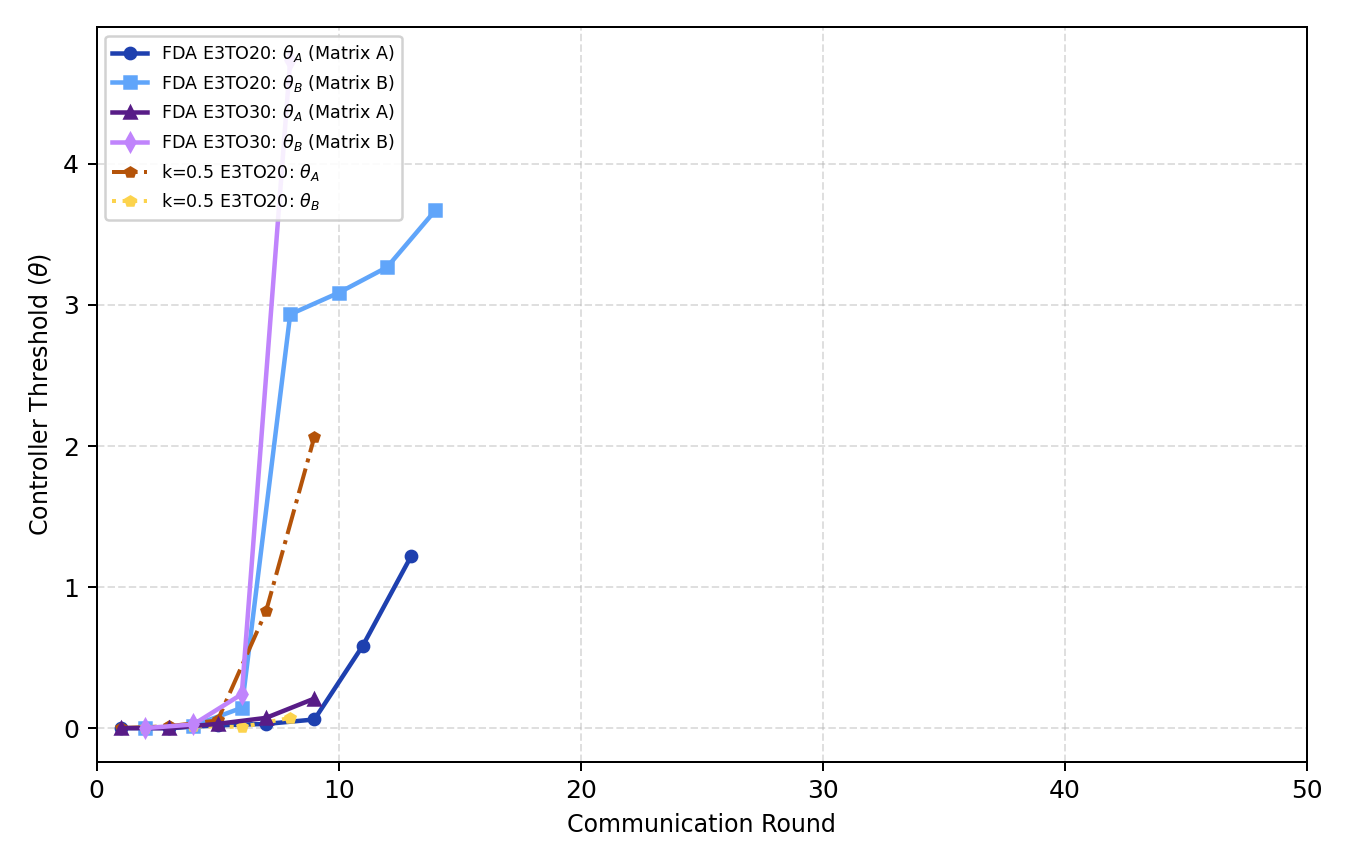
\includegraphics[width=\textwidth,height=4.9cm,keepaspectratio]{figures/telemetry/09_QQP_C20_R50_LR0.1_5_fda_threshold.png}
            \vspace{2pt}
            \par{\footnotesize \textbf{(d)} Factor Thresholds ($\theta_A, \theta_B$)}
        \end{minipage}

        \vspace{0.6em}
        \begin{minipage}[b]{0.485\textwidth}
            \centering
            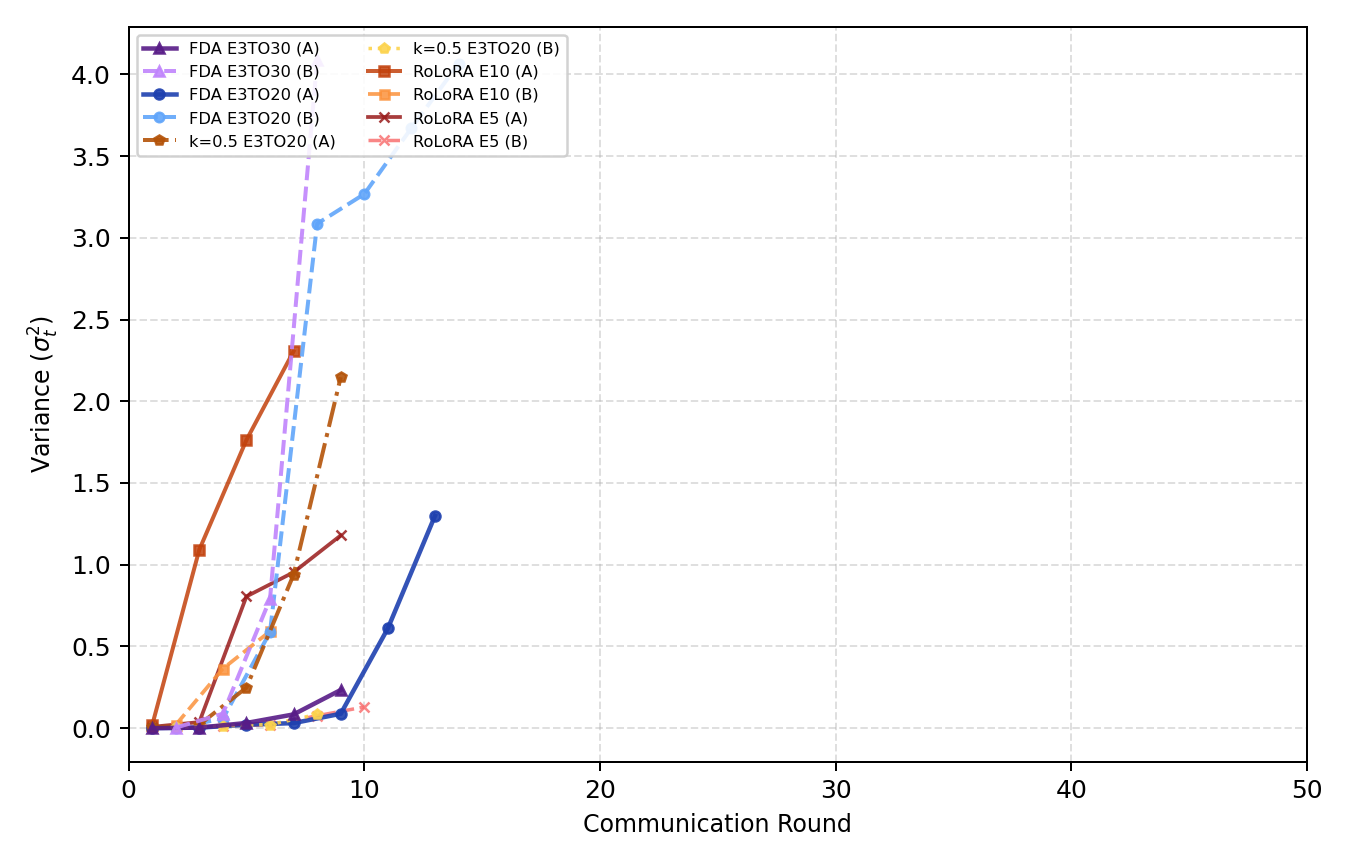
\includegraphics[width=\textwidth,height=4.9cm,keepaspectratio]{figures/telemetry/09_QQP_C20_R50_LR0.1_3_client_variance.png}
            \vspace{2pt}
            \par{\footnotesize \textbf{(e)} Subspace Coordinate Variance}
        \end{minipage}\hfill
        \begin{minipage}[b]{0.485\textwidth}
            \centering
            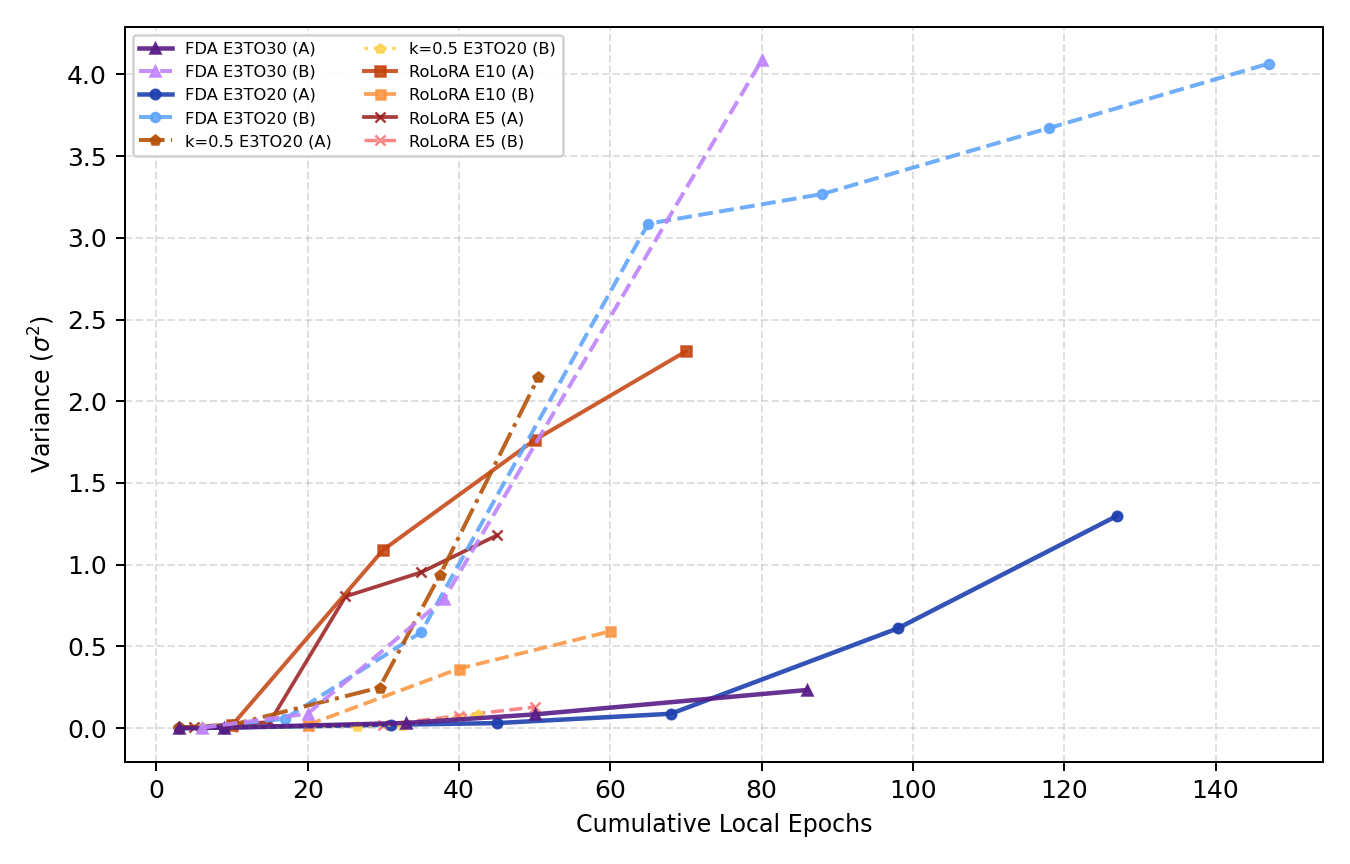
\includegraphics[width=\textwidth,height=4.9cm,keepaspectratio]{figures/telemetry/09_QQP_C20_R50_LR0.1_6_variance_vs_epoch.png}
            \vspace{2pt}
            \par{\footnotesize \textbf{(f)} Variance vs.\ Cumulative Local Epochs}
        \end{minipage}

        \vspace{0.6em}
        \caption{Multi-panel optimization telemetry on QQP ($C=20, R_{\max}=50, \eta_c=0.1, \alpha=1000.0$) comparing FDA-RoLoRA against static RoLoRA baselines under homogeneous consensus.}
        \label{fig:telemetry_qqp_c20_iid}
    \end{minipage}%
    }
\end{figure}

\begin{figure}[p]
    \centering
    \makebox[\textwidth][c]{%
    \begin{minipage}{1.06\textwidth}
        \begin{minipage}[b]{0.485\textwidth}
            \centering
            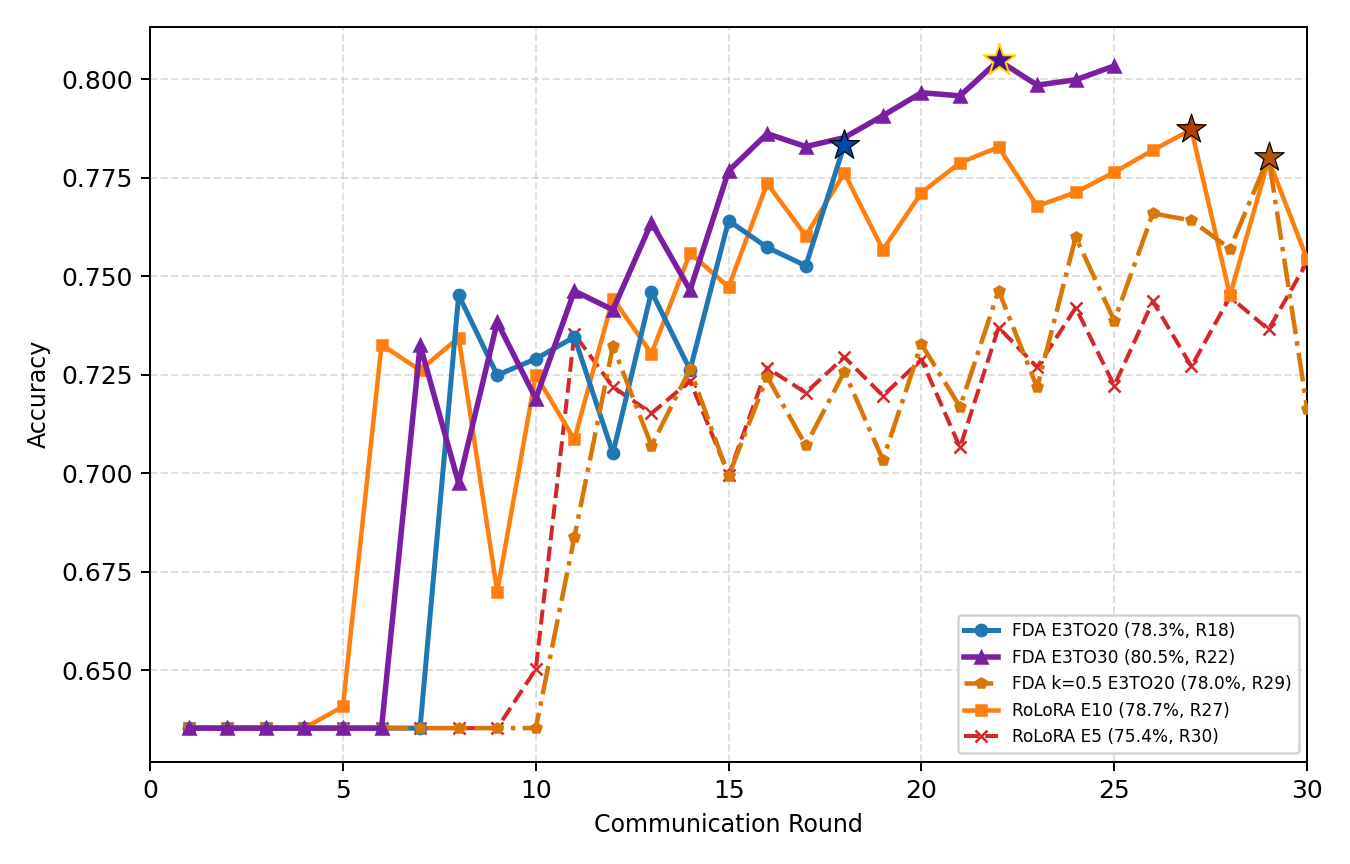
\includegraphics[width=\textwidth,height=4.9cm,keepaspectratio]{figures/telemetry/10_QQP_C50_R30_LR0.1_1_accuracy.png}
            \vspace{2pt}
            \par{\footnotesize \textbf{(a)} Validation Accuracy}
        \end{minipage}\hfill
        \begin{minipage}[b]{0.485\textwidth}
            \centering
            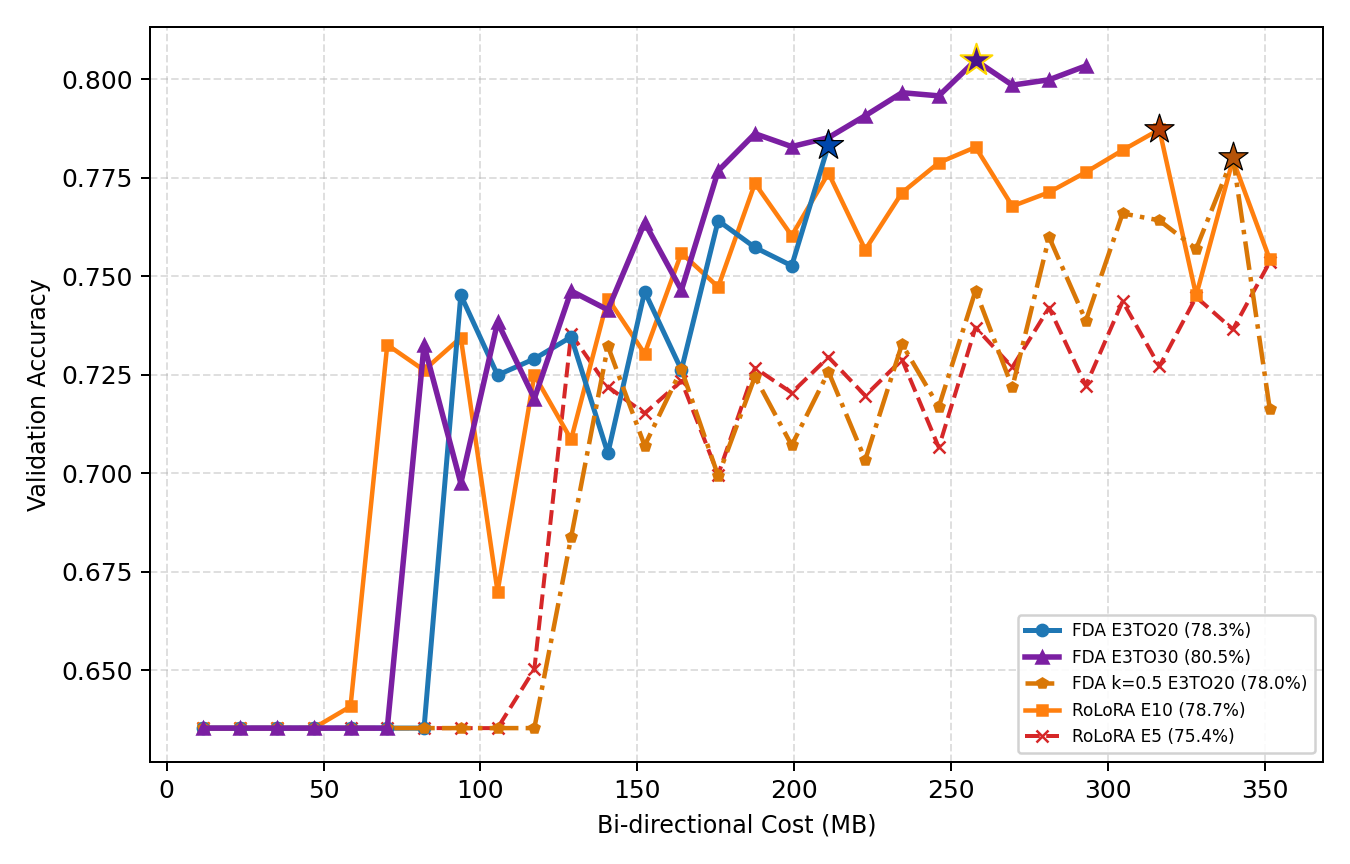
\includegraphics[width=\textwidth,height=4.9cm,keepaspectratio]{figures/telemetry/10_QQP_C50_R30_LR0.1_4_accuracy_vs_cost.png}
            \vspace{2pt}
            \par{\footnotesize \textbf{(b)} Accuracy vs. Communication (MB)}
        \end{minipage}

        \vspace{0.6em}
        \begin{minipage}[b]{0.485\textwidth}
            \centering
            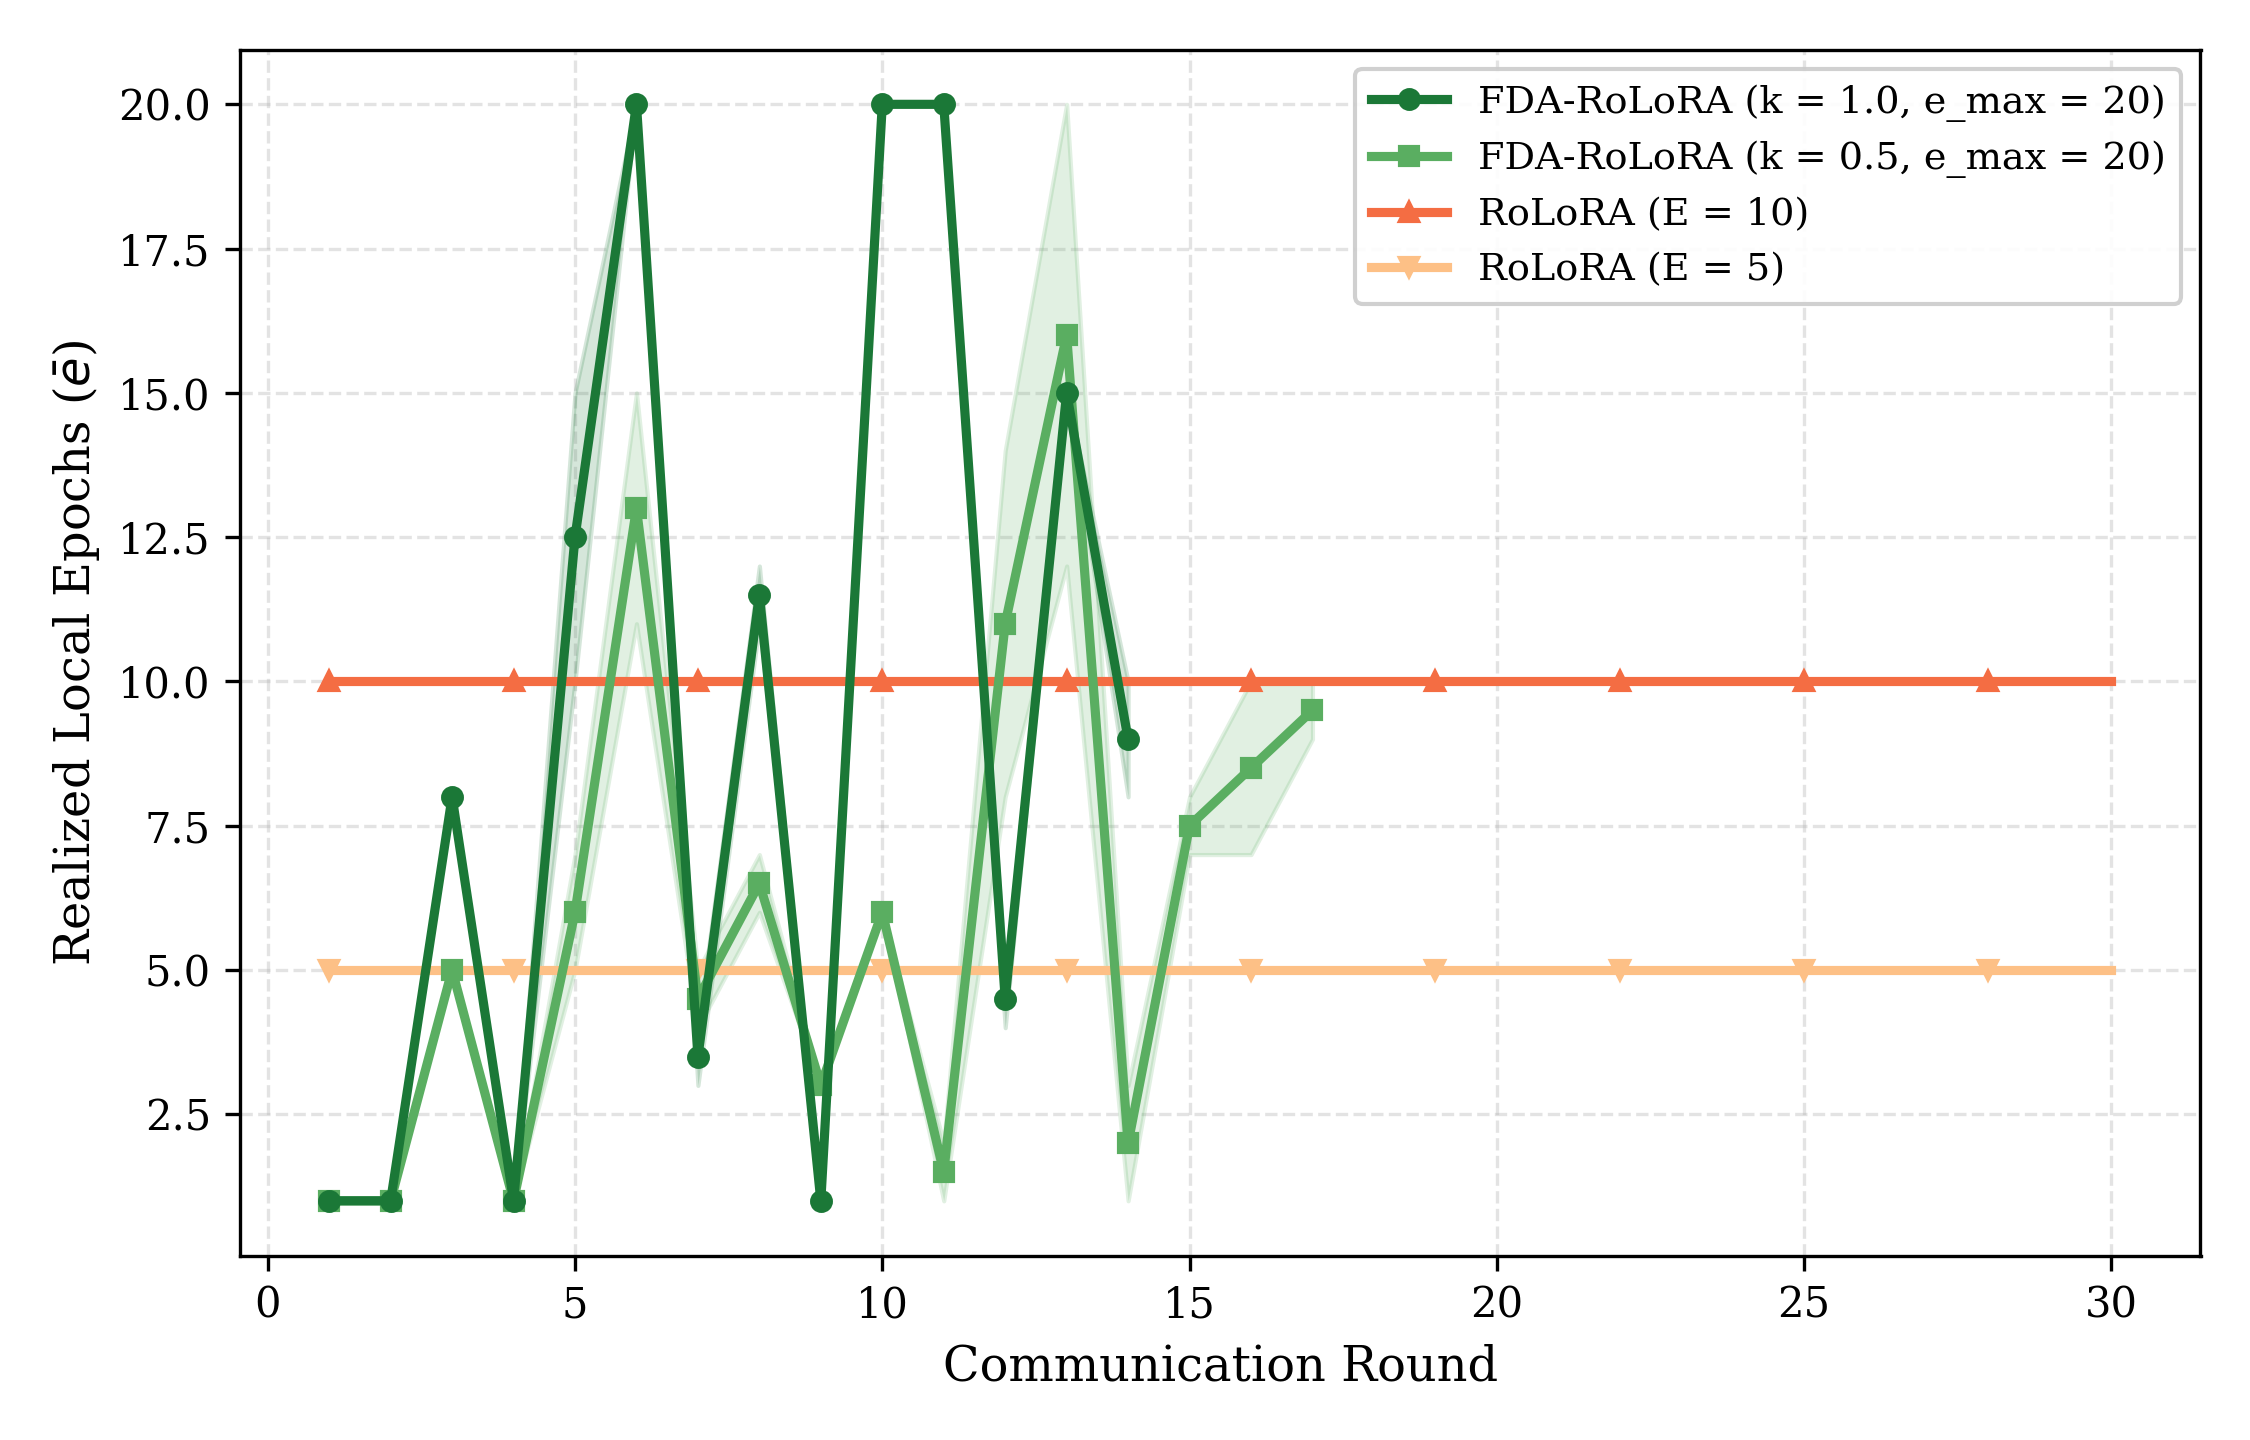
\includegraphics[width=\textwidth,height=4.9cm,keepaspectratio]{figures/telemetry/10_QQP_C50_R30_LR0.1_2_allocated_epochs.png}
            \vspace{2pt}
            \par{\footnotesize \textbf{(c)} Dynamic Local Epochs ($\bar{e}$)}
        \end{minipage}\hfill
        \begin{minipage}[b]{0.485\textwidth}
            \centering
            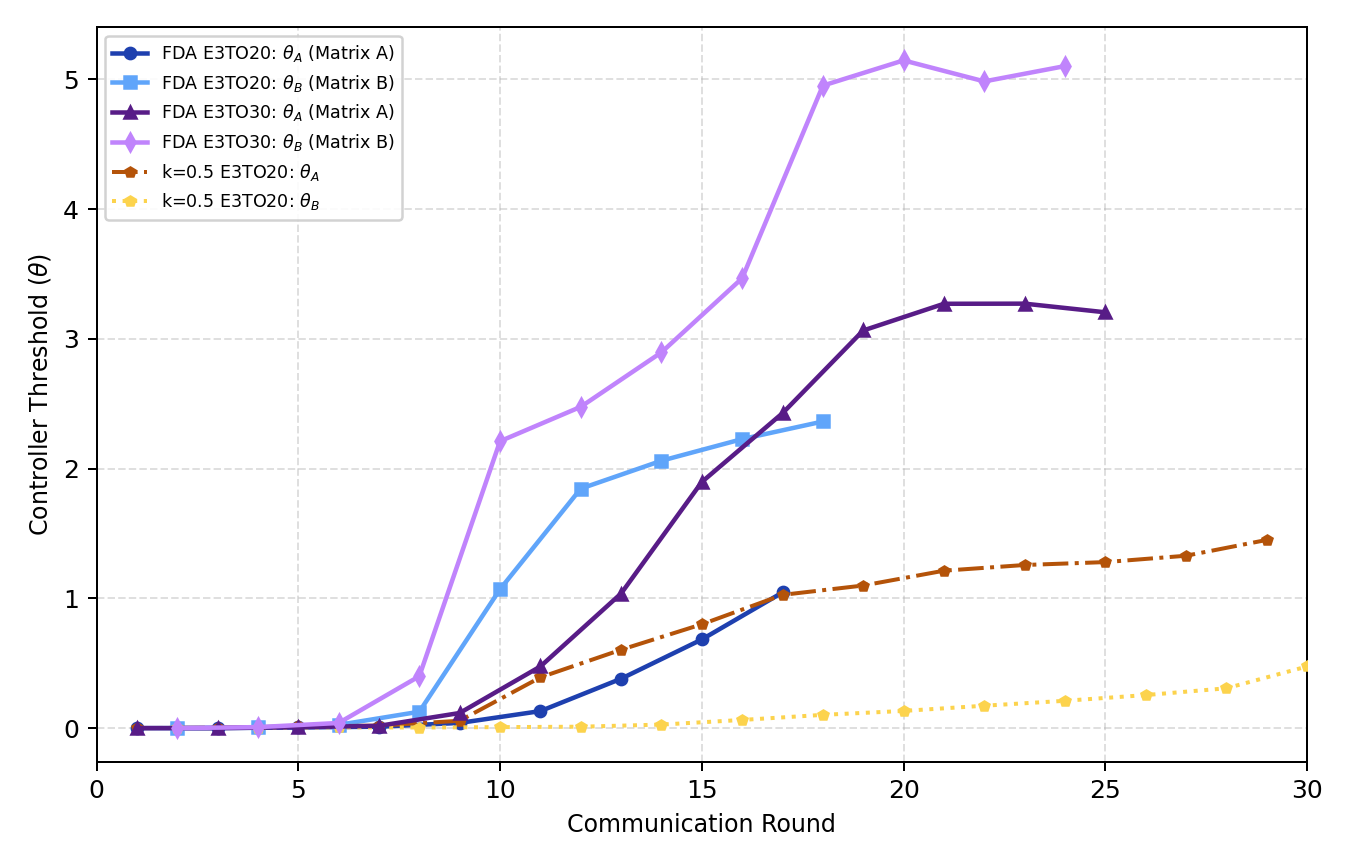
\includegraphics[width=\textwidth,height=4.9cm,keepaspectratio]{figures/telemetry/10_QQP_C50_R30_LR0.1_5_fda_threshold.png}
            \vspace{2pt}
            \par{\footnotesize \textbf{(d)} Factor Thresholds ($\theta_A, \theta_B$)}
        \end{minipage}

        \vspace{0.6em}
        \begin{minipage}[b]{0.485\textwidth}
            \centering
            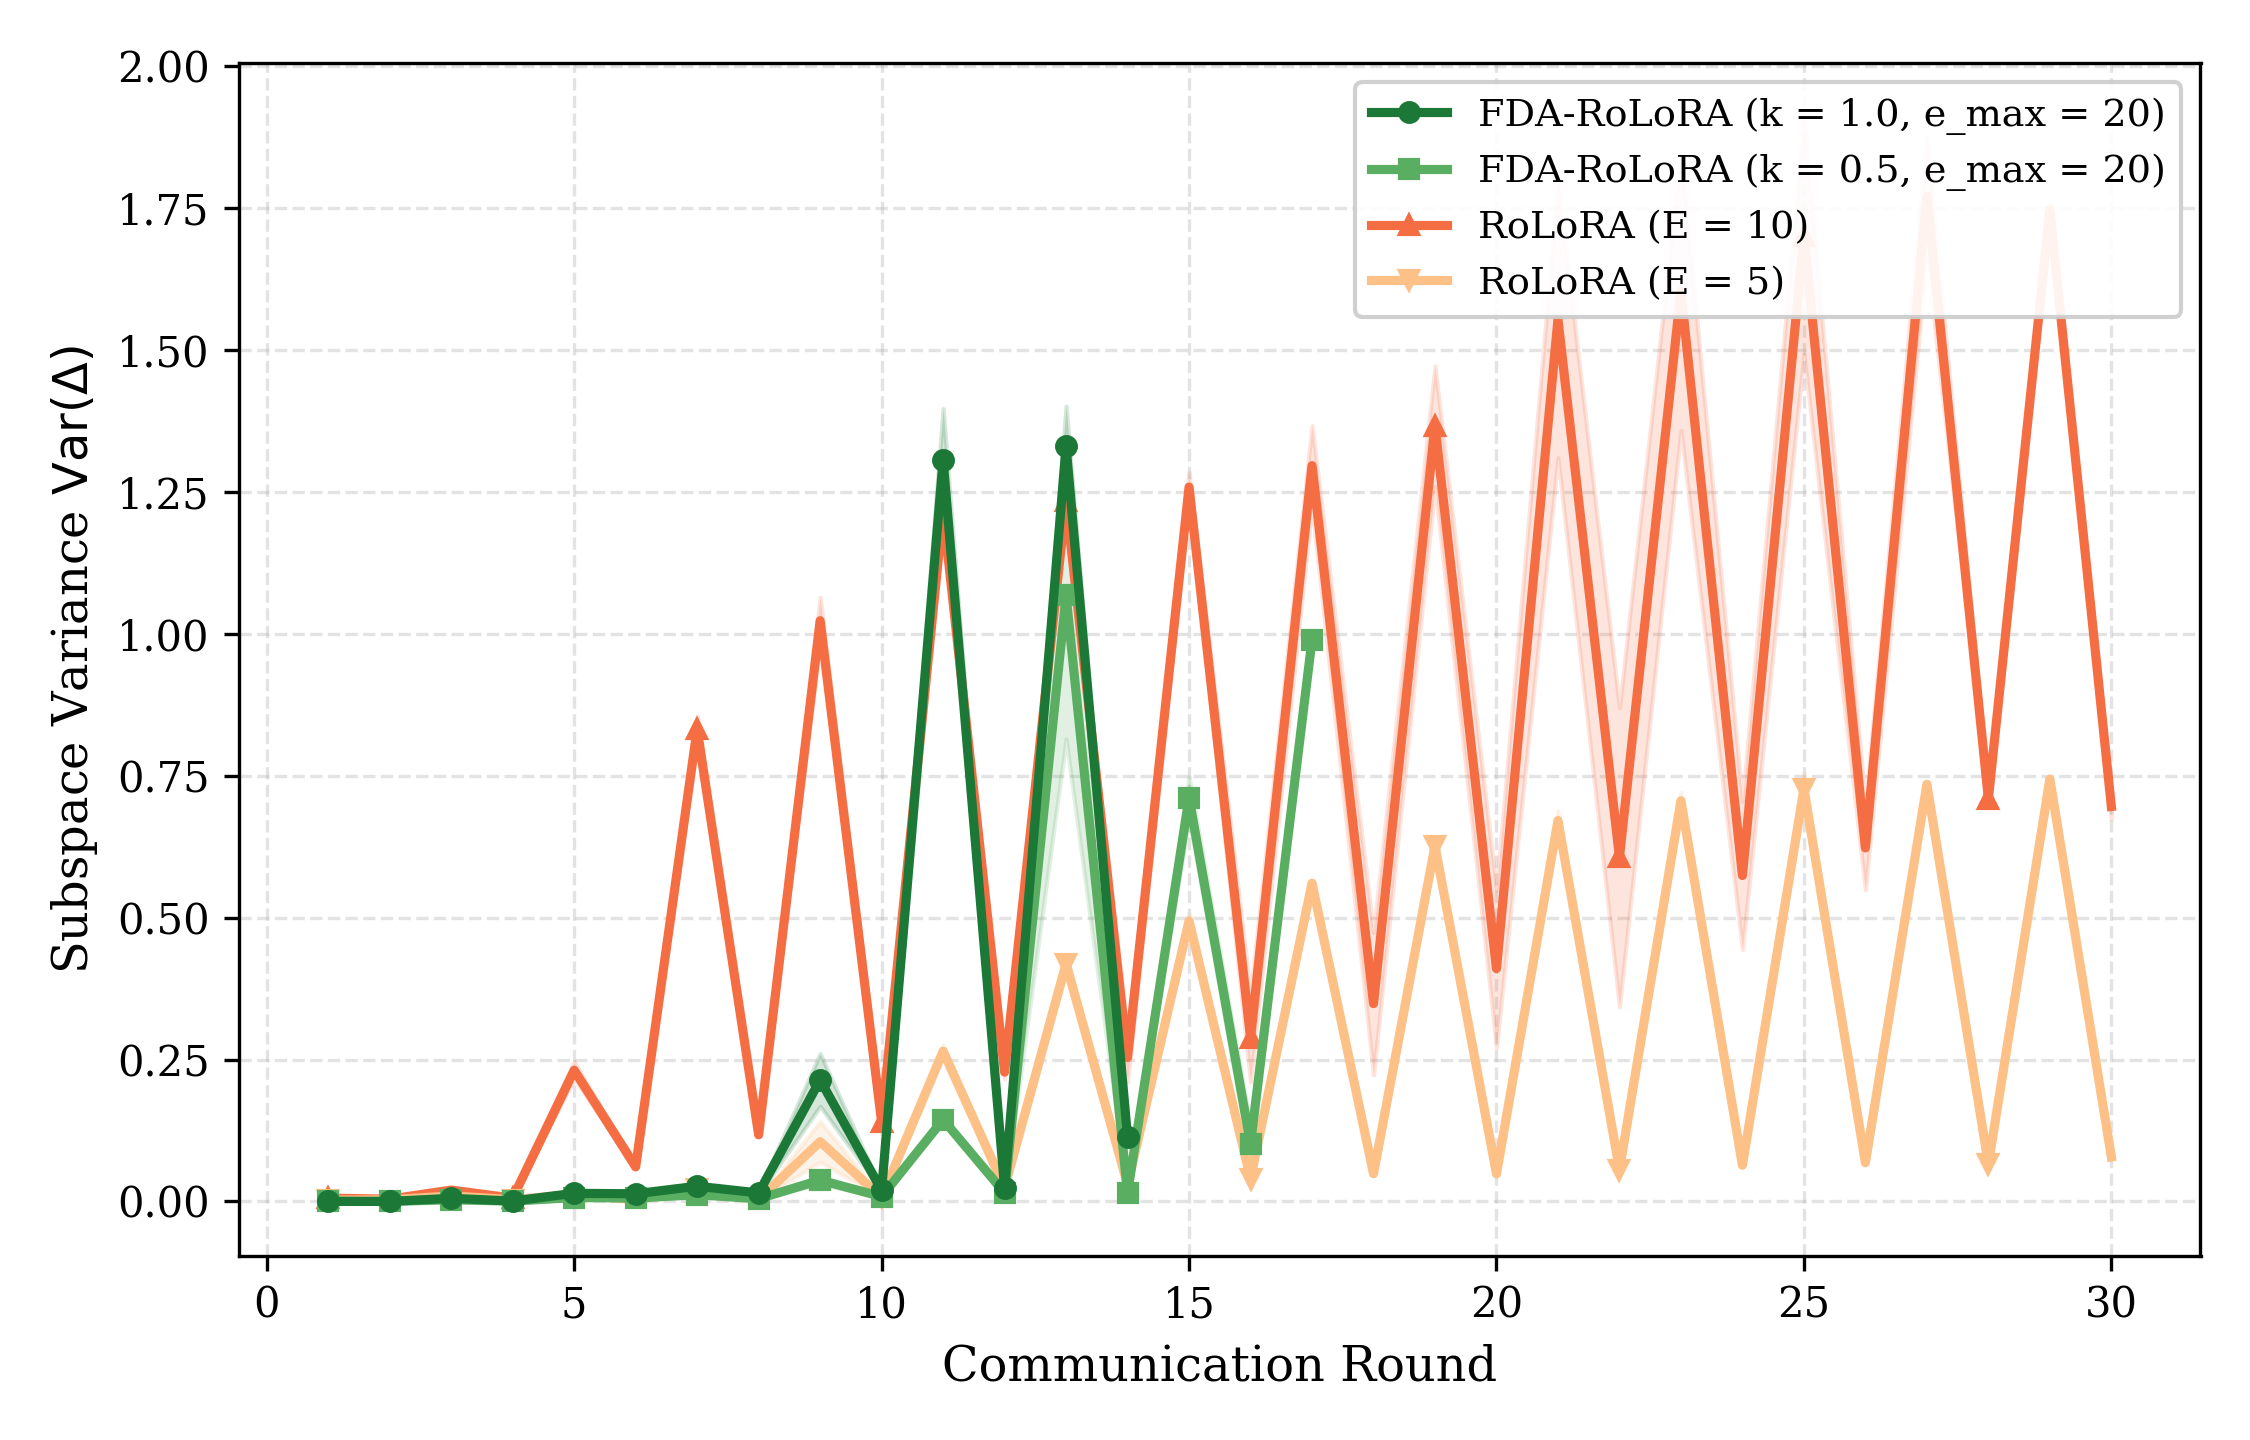
\includegraphics[width=\textwidth,height=4.9cm,keepaspectratio]{figures/telemetry/10_QQP_C50_R30_LR0.1_3_client_variance.png}
            \vspace{2pt}
            \par{\footnotesize \textbf{(e)} Subspace Coordinate Variance}
        \end{minipage}\hfill
        \begin{minipage}[b]{0.485\textwidth}
            \centering
            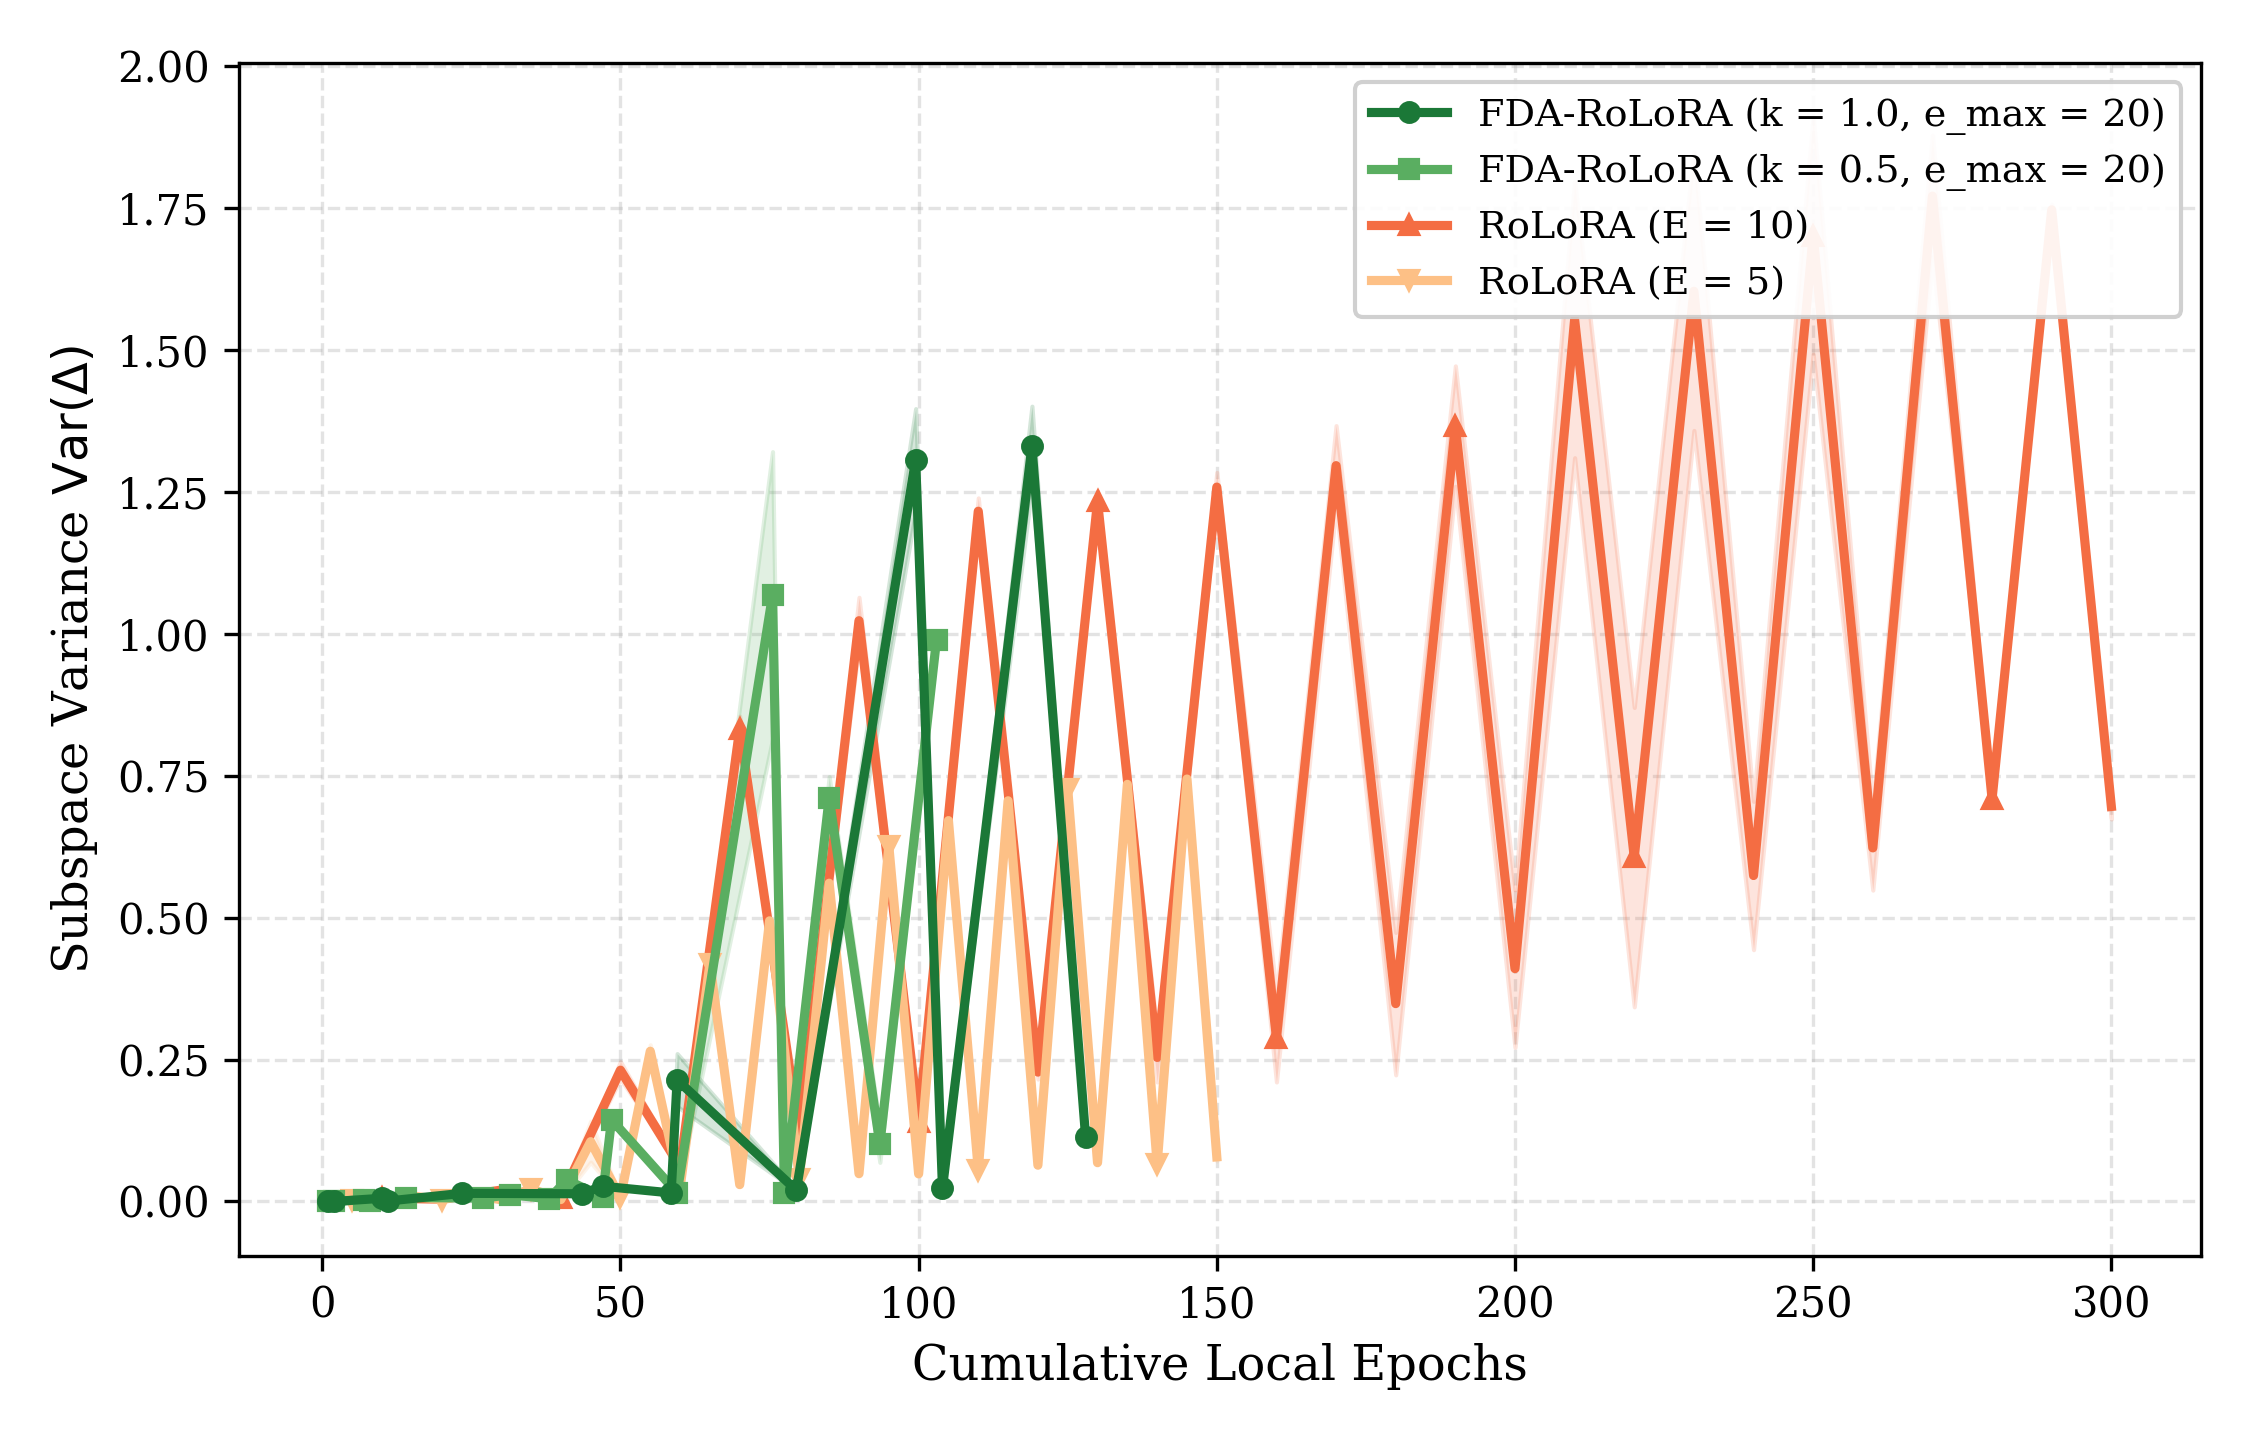
\includegraphics[width=\textwidth,height=4.9cm,keepaspectratio]{figures/telemetry/10_QQP_C50_R30_LR0.1_6_variance_vs_epoch.png}
            \vspace{2pt}
            \par{\footnotesize \textbf{(f)} Variance vs.\ Cumulative Local Epochs}
        \end{minipage}

        \vspace{0.6em}
        \caption{Multi-panel optimization telemetry on QQP ($C=50, R_{\max}=30, \eta_c=0.1, \alpha=1000.0$) under expanded cohort scale $C=50$.}
        \label{fig:telemetry_qqp_c50_iid}
    \end{minipage}%
    }
\end{figure}

\paragraph{SST-2:}
Figures~\ref{fig:telemetry_sst2_c20_iid} and \ref{fig:telemetry_sst2_c50_iid} report telemetry on single-sentence sentiment classification under homogeneous consensus. On $C=20$ (Figure~\ref{fig:telemetry_sst2_c20_iid}), both FDA-RoLoRA and fixed RoLoRA rapidly cross $92\%$ validation accuracy (Panel a). FDA-RoLoRA ($k=1.0$) reaches a peak of $92.14\%$, close to RoLoRA $E=20$ ($92.55\%$), but uses more communication ($57.7\,\text{MB}$ vs.\ $30.0\,\text{MB}$). Realized local epochs (Panel c) settle at $\bar{e} = 11.11$ per round, while dual thresholds (Panel d) stabilize at tight equilibria. Round-level drift variance (Panel e) is bounded at $\bar{\nu} = 0.654$.

On $C=50$ (Figure~\ref{fig:telemetry_sst2_c50_iid}), FDA-RoLoRA ($k=1.0$) achieves $89.68\%$ validation accuracy in $20.0$ rounds ($140.6\,\text{MB}$) versus $22.0$ rounds ($154.7\,\text{MB}$) for static RoLoRA $E=10$ (Panels a \& b), at lower accuracy than RoLoRA $E=10$ ($90.54\%$ peak) and $E=20$ ($92.01\%$ peak). Cohort aggregation suppresses coordinate drift variance to a low $\bar{\nu} = 0.063$ (Panel e).
\begin{figure}[p]
    \centering
    \makebox[\textwidth][c]{%
    \begin{minipage}{1.06\textwidth}
        \begin{minipage}[b]{0.485\textwidth}
            \centering
            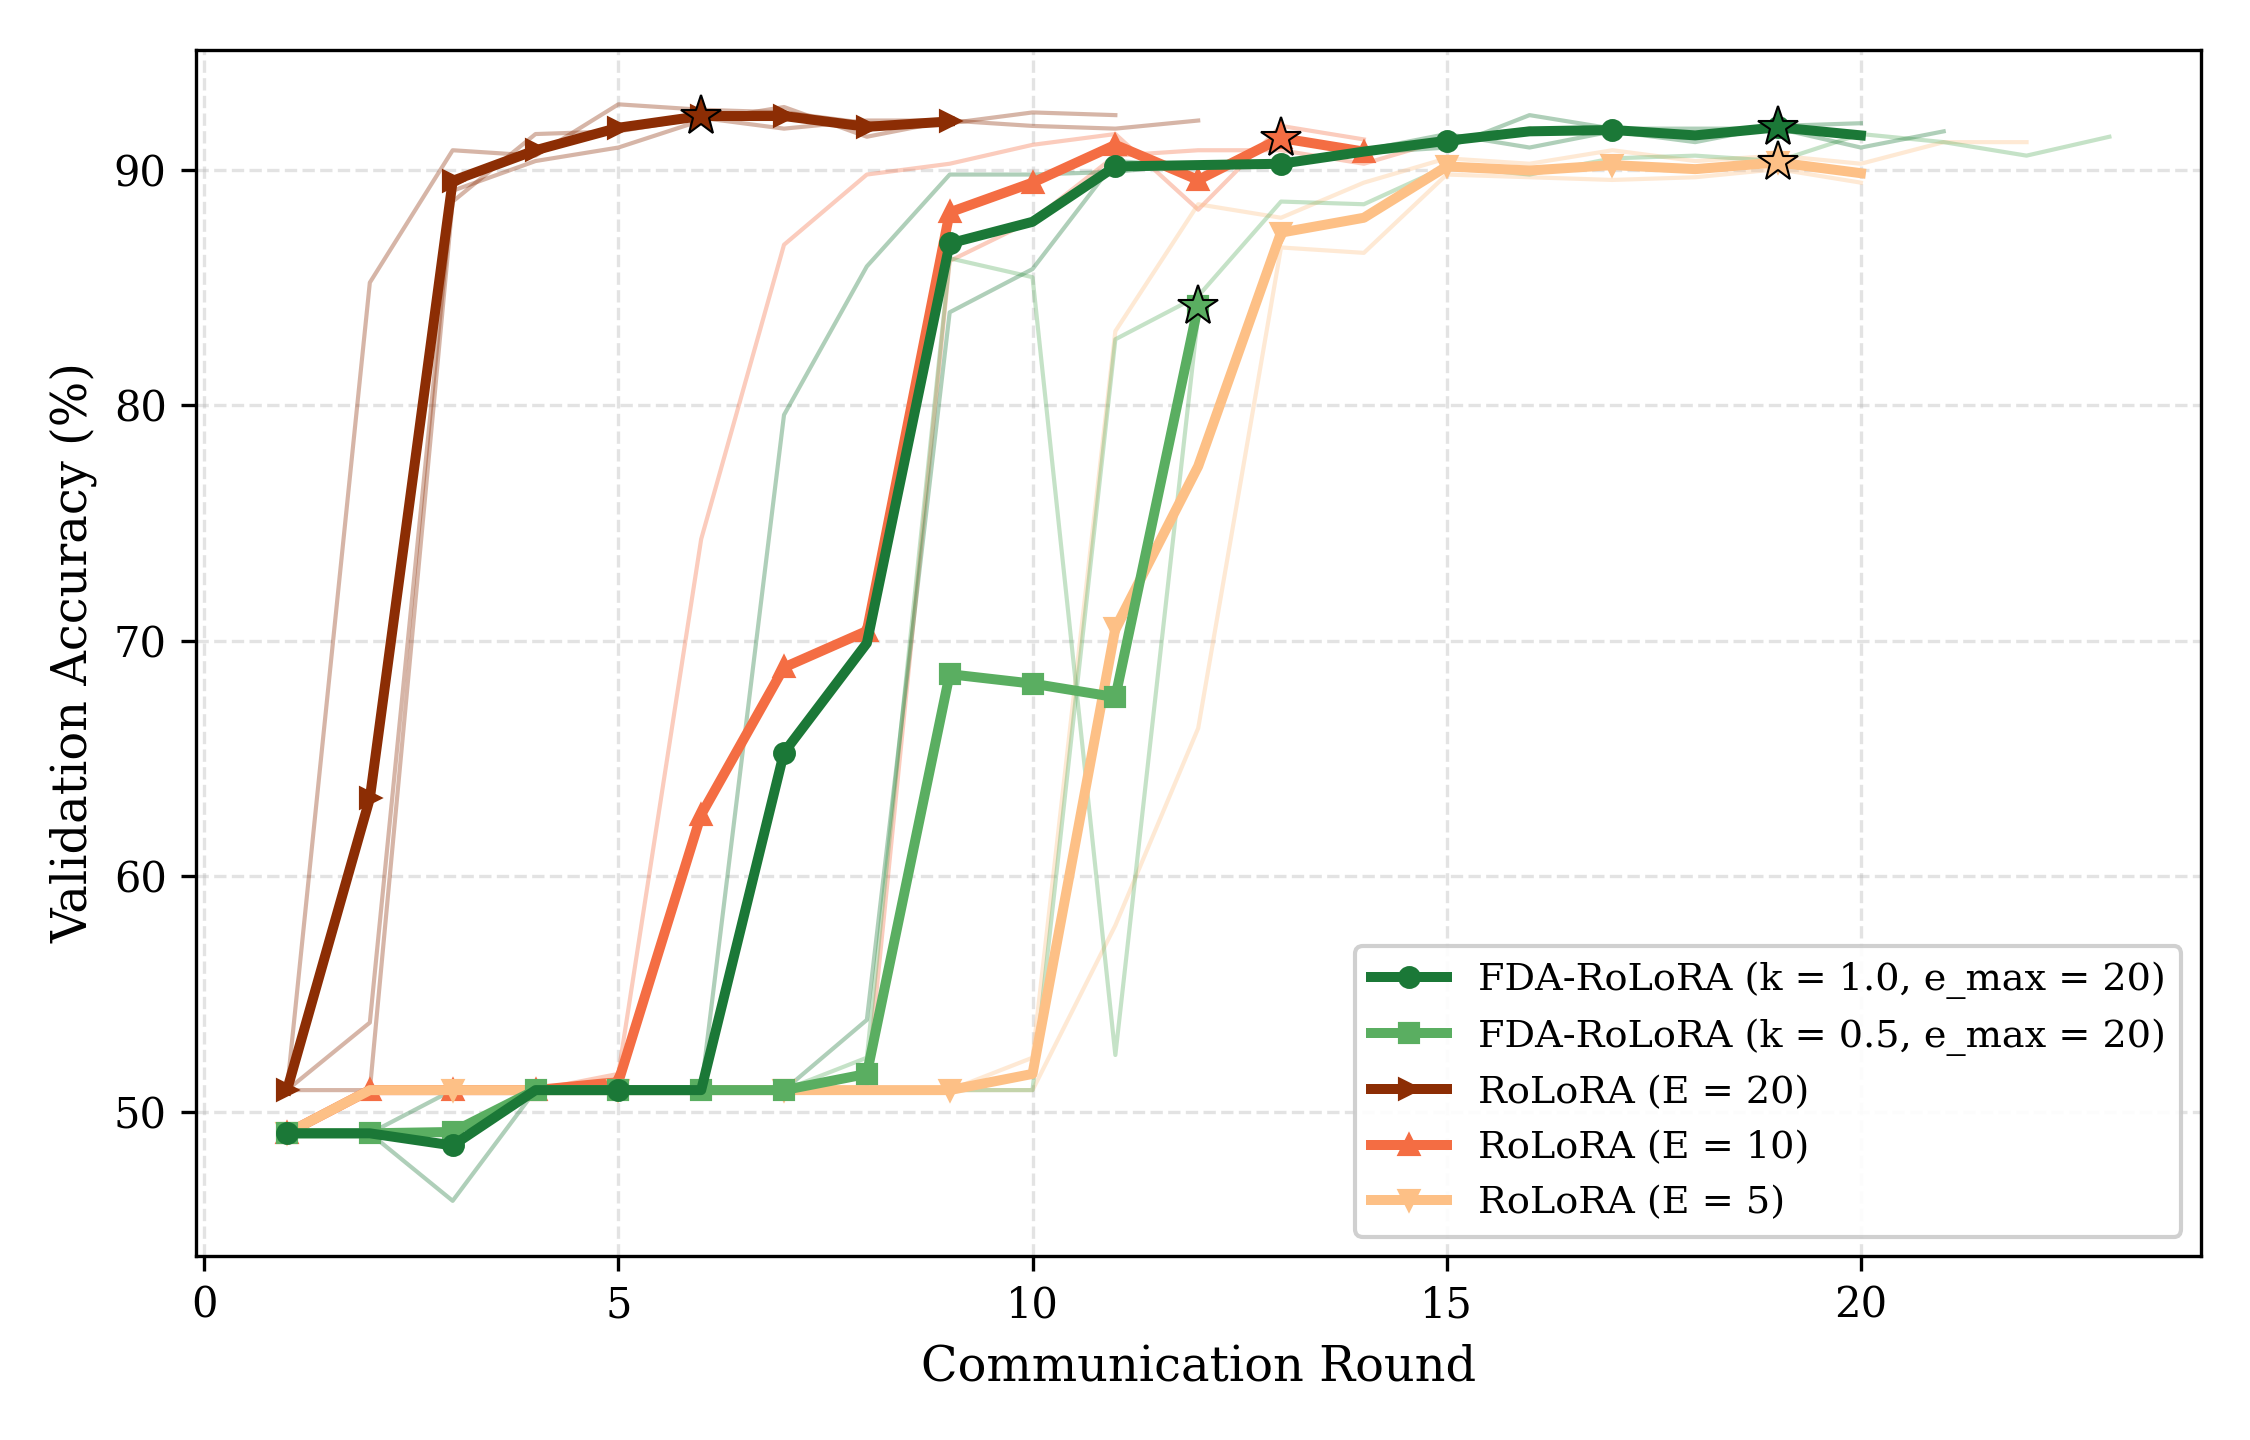
\includegraphics[width=\textwidth,height=4.9cm,keepaspectratio]{figures/telemetry/11_SST2_C20_R50_LR0.1_1_accuracy.png}
            \vspace{2pt}
            \par{\footnotesize \textbf{(a)} Validation Accuracy}
        \end{minipage}\hfill
        \begin{minipage}[b]{0.485\textwidth}
            \centering
            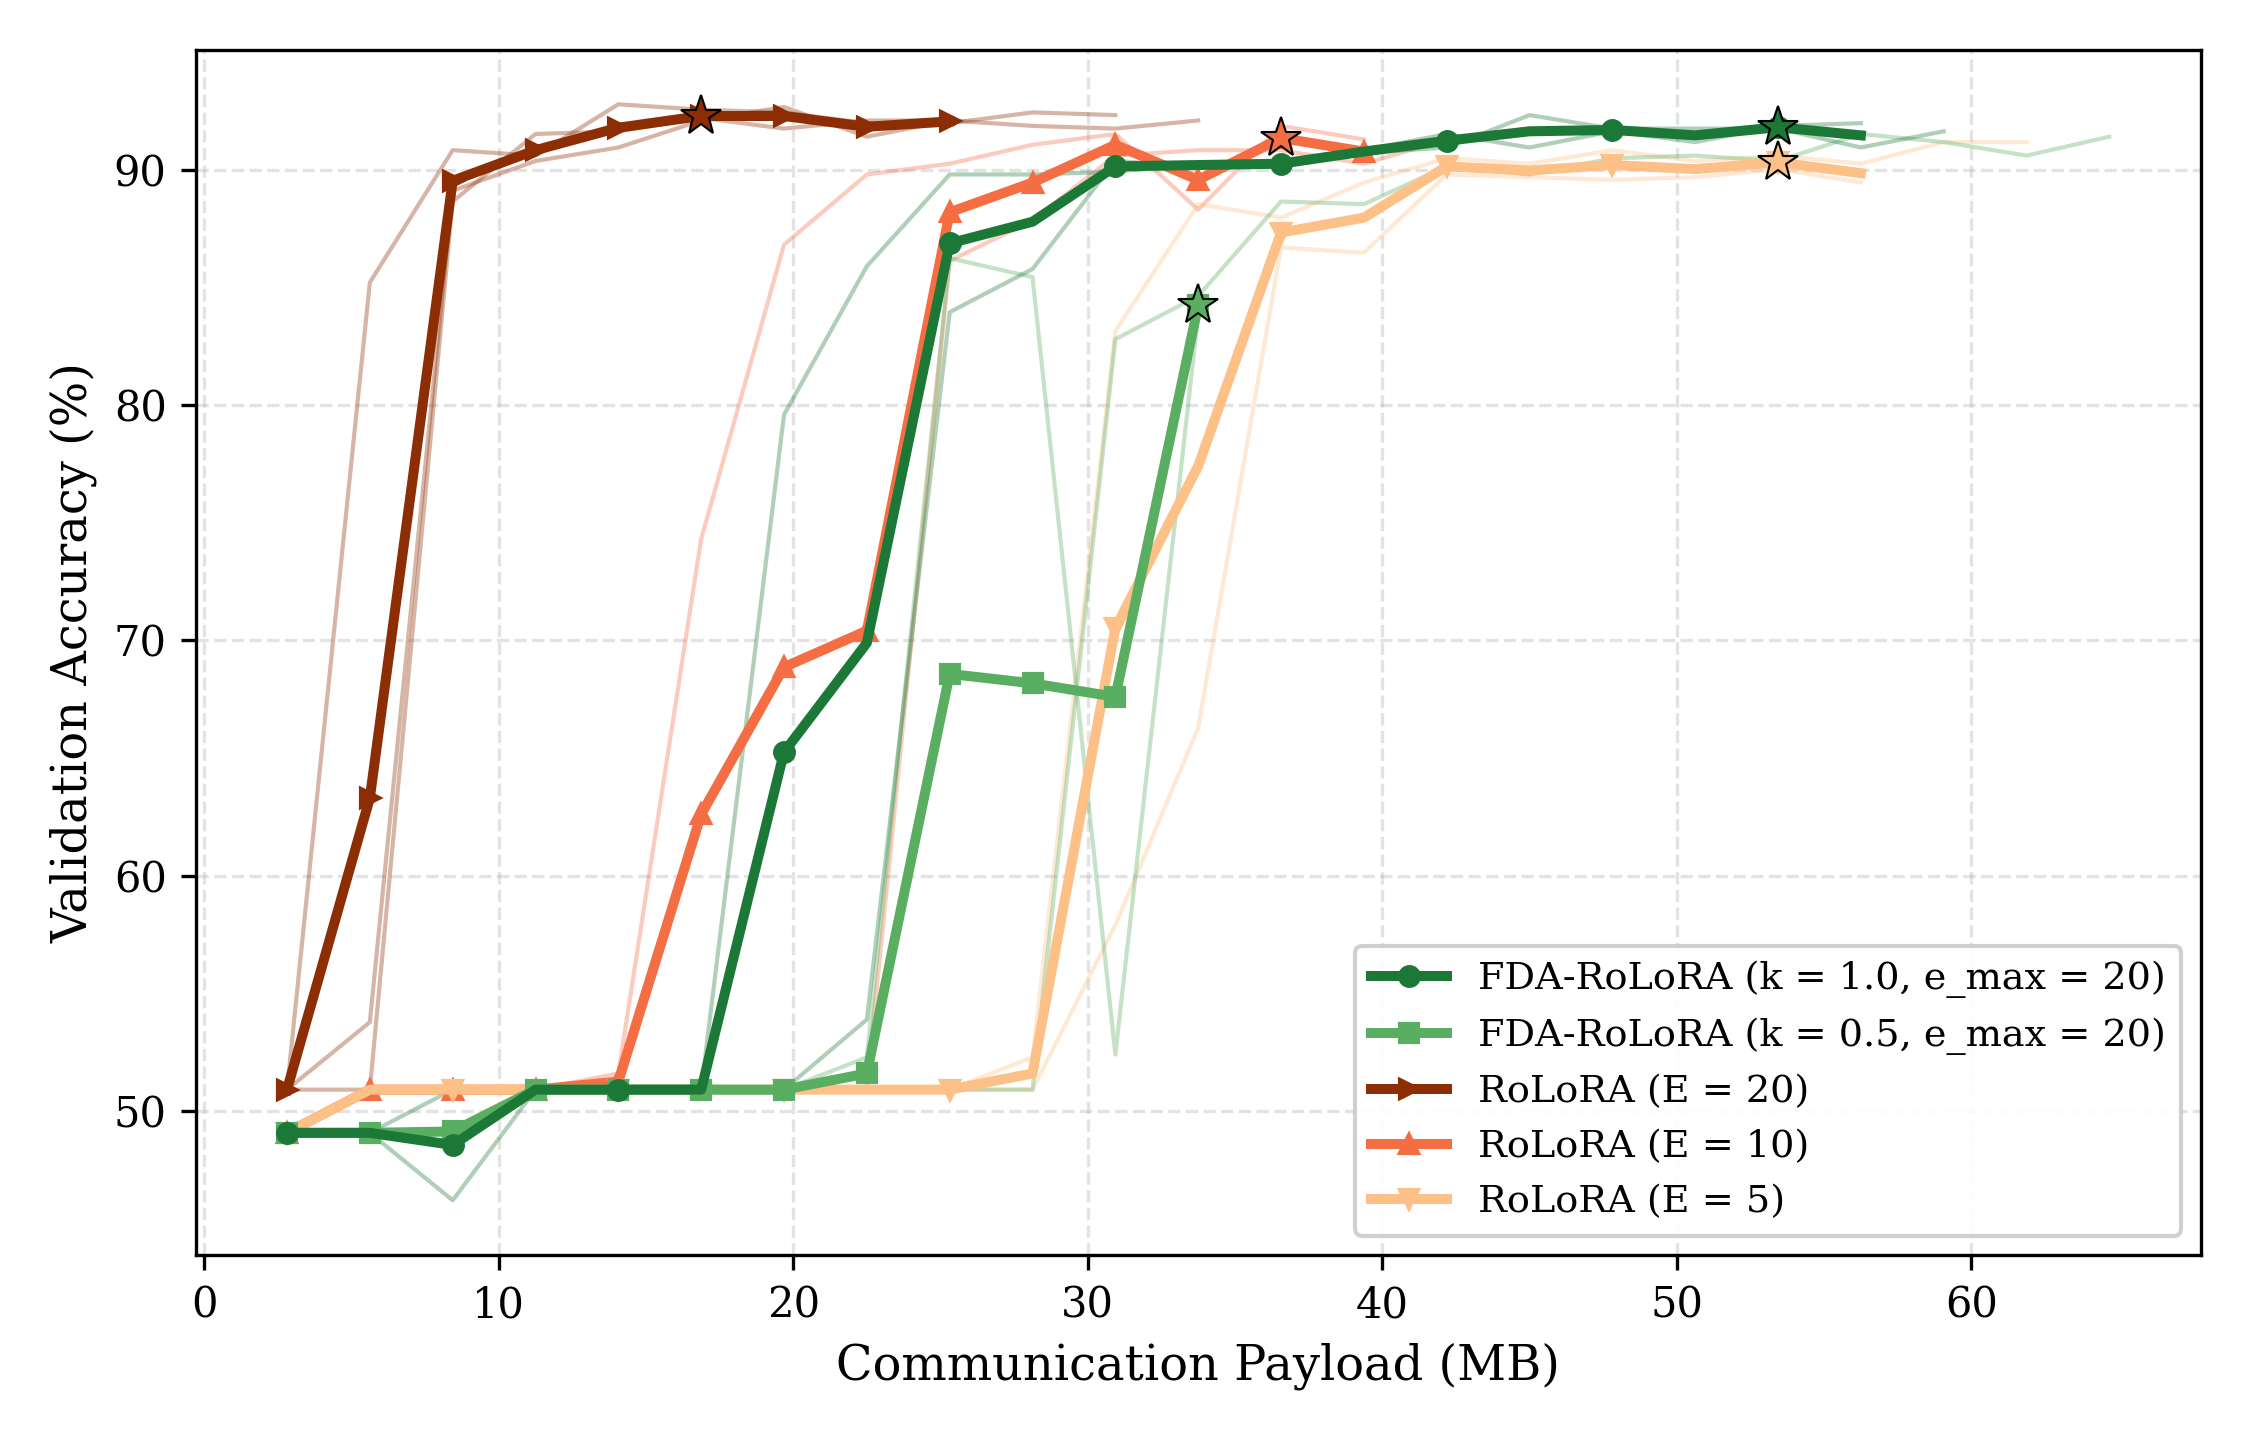
\includegraphics[width=\textwidth,height=4.9cm,keepaspectratio]{figures/telemetry/11_SST2_C20_R50_LR0.1_4_accuracy_vs_cost.png}
            \vspace{2pt}
            \par{\footnotesize \textbf{(b)} Accuracy vs. Communication (MB)}
        \end{minipage}

        \vspace{0.6em}
        \begin{minipage}[b]{0.485\textwidth}
            \centering
            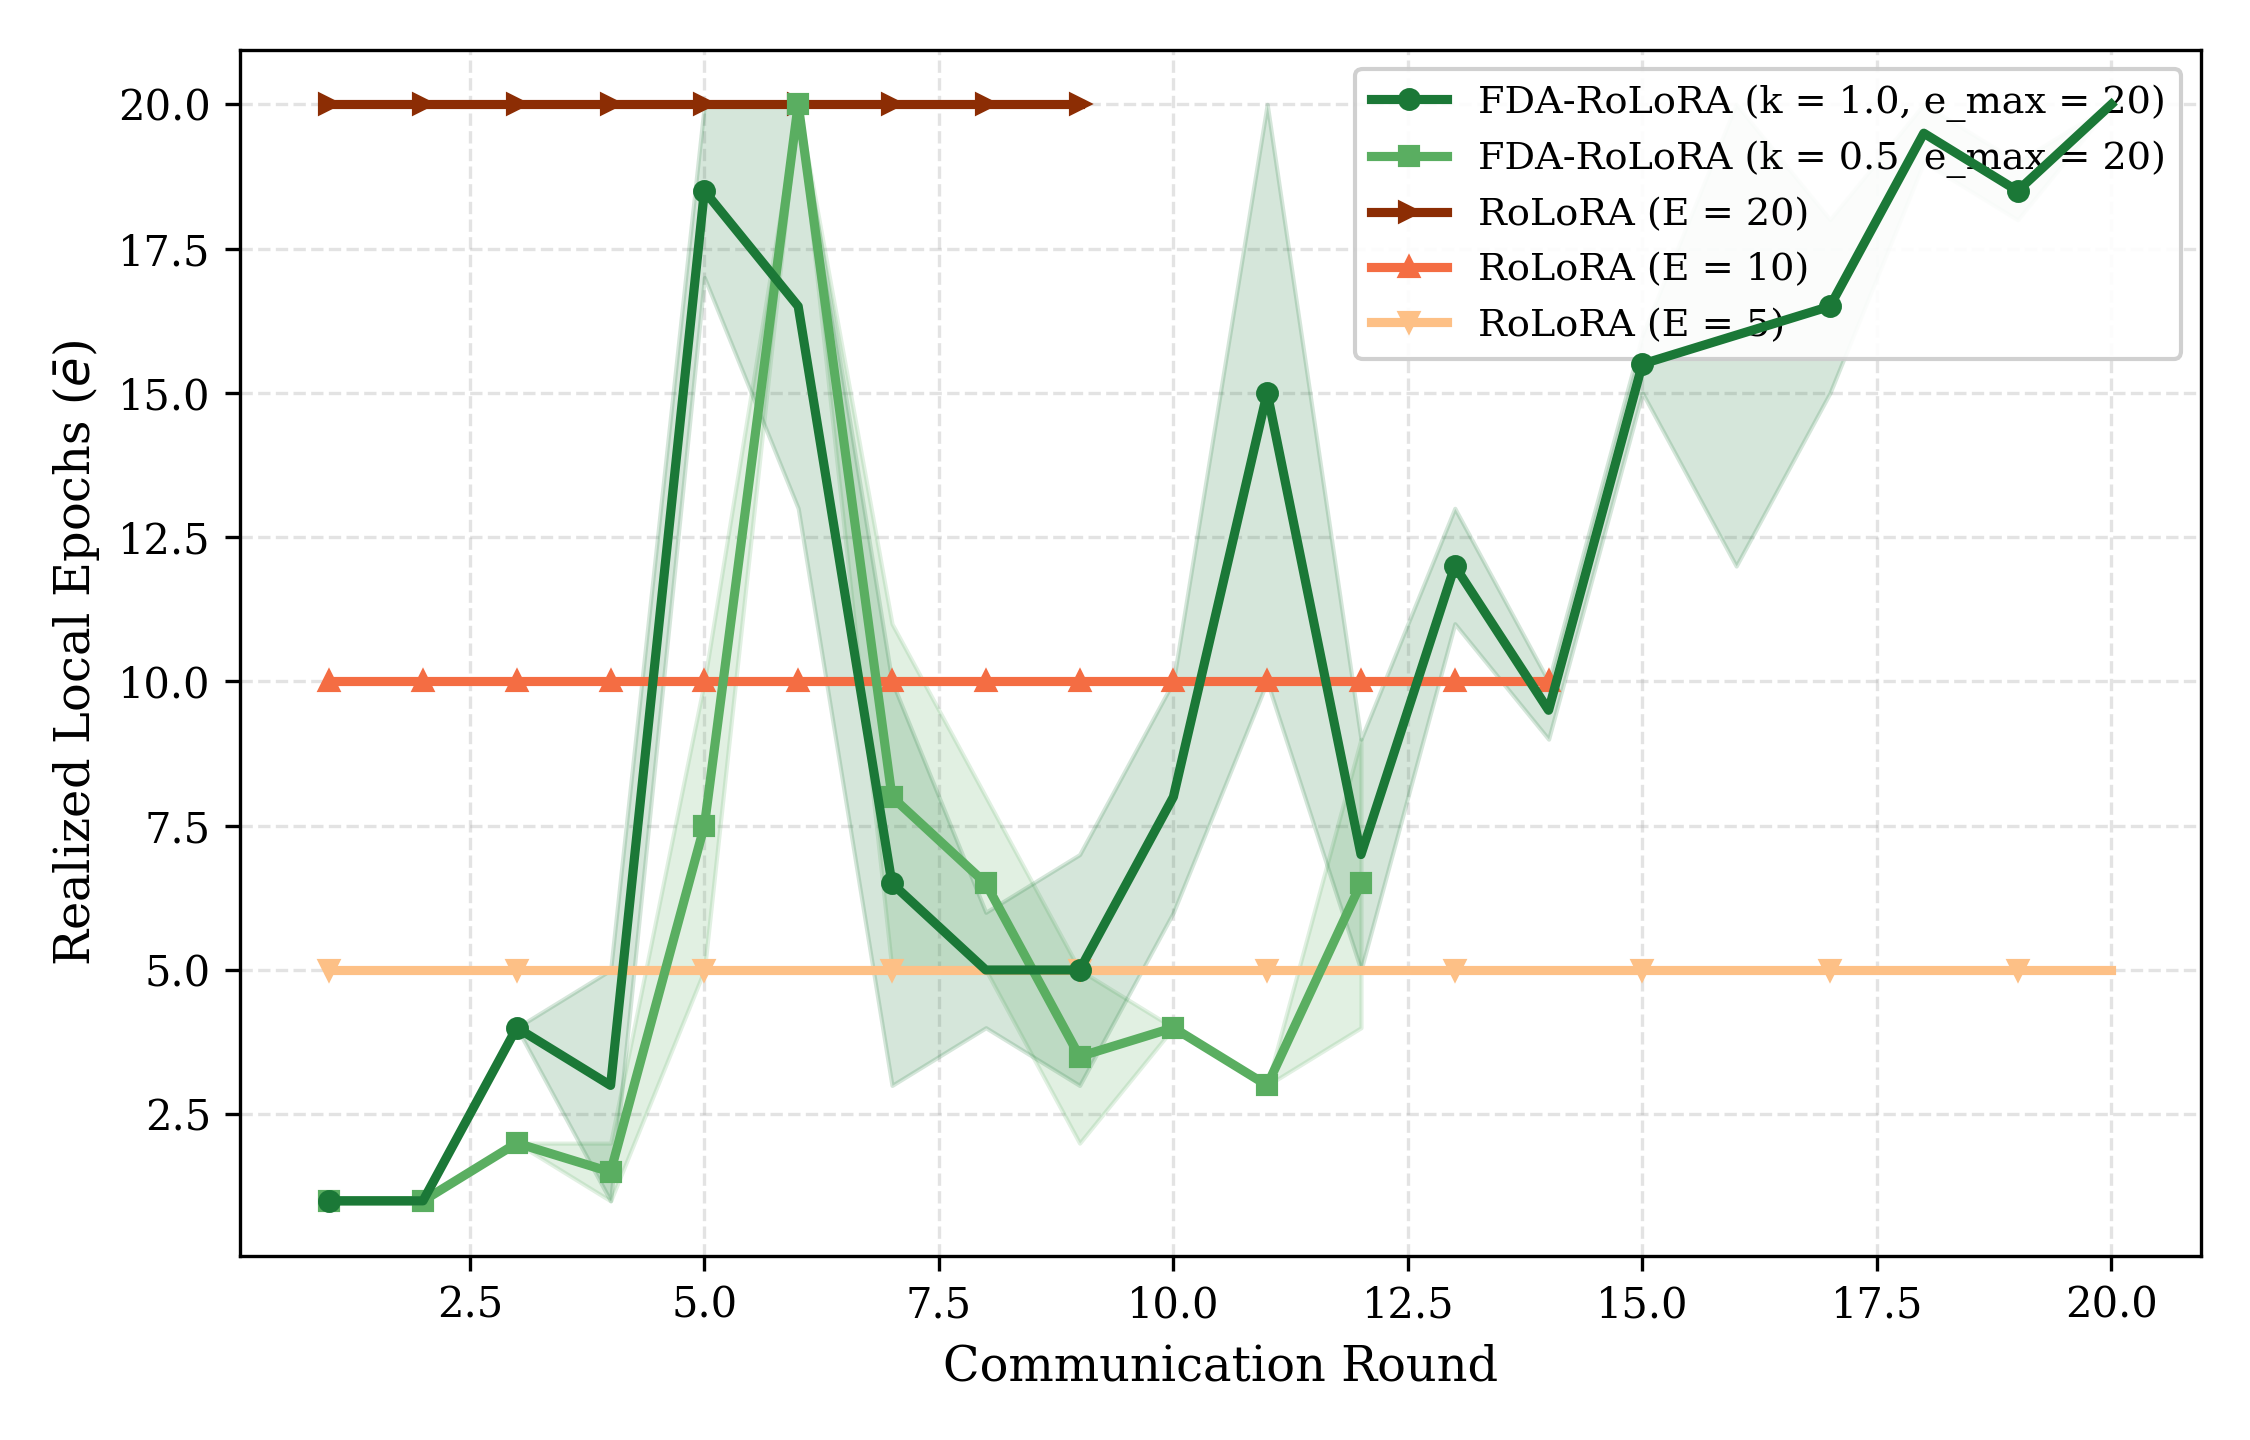
\includegraphics[width=\textwidth,height=4.9cm,keepaspectratio]{figures/telemetry/11_SST2_C20_R50_LR0.1_2_allocated_epochs.png}
            \vspace{2pt}
            \par{\footnotesize \textbf{(c)} Dynamic Local Epochs ($\bar{e}$)}
        \end{minipage}\hfill
        \begin{minipage}[b]{0.485\textwidth}
            \centering
            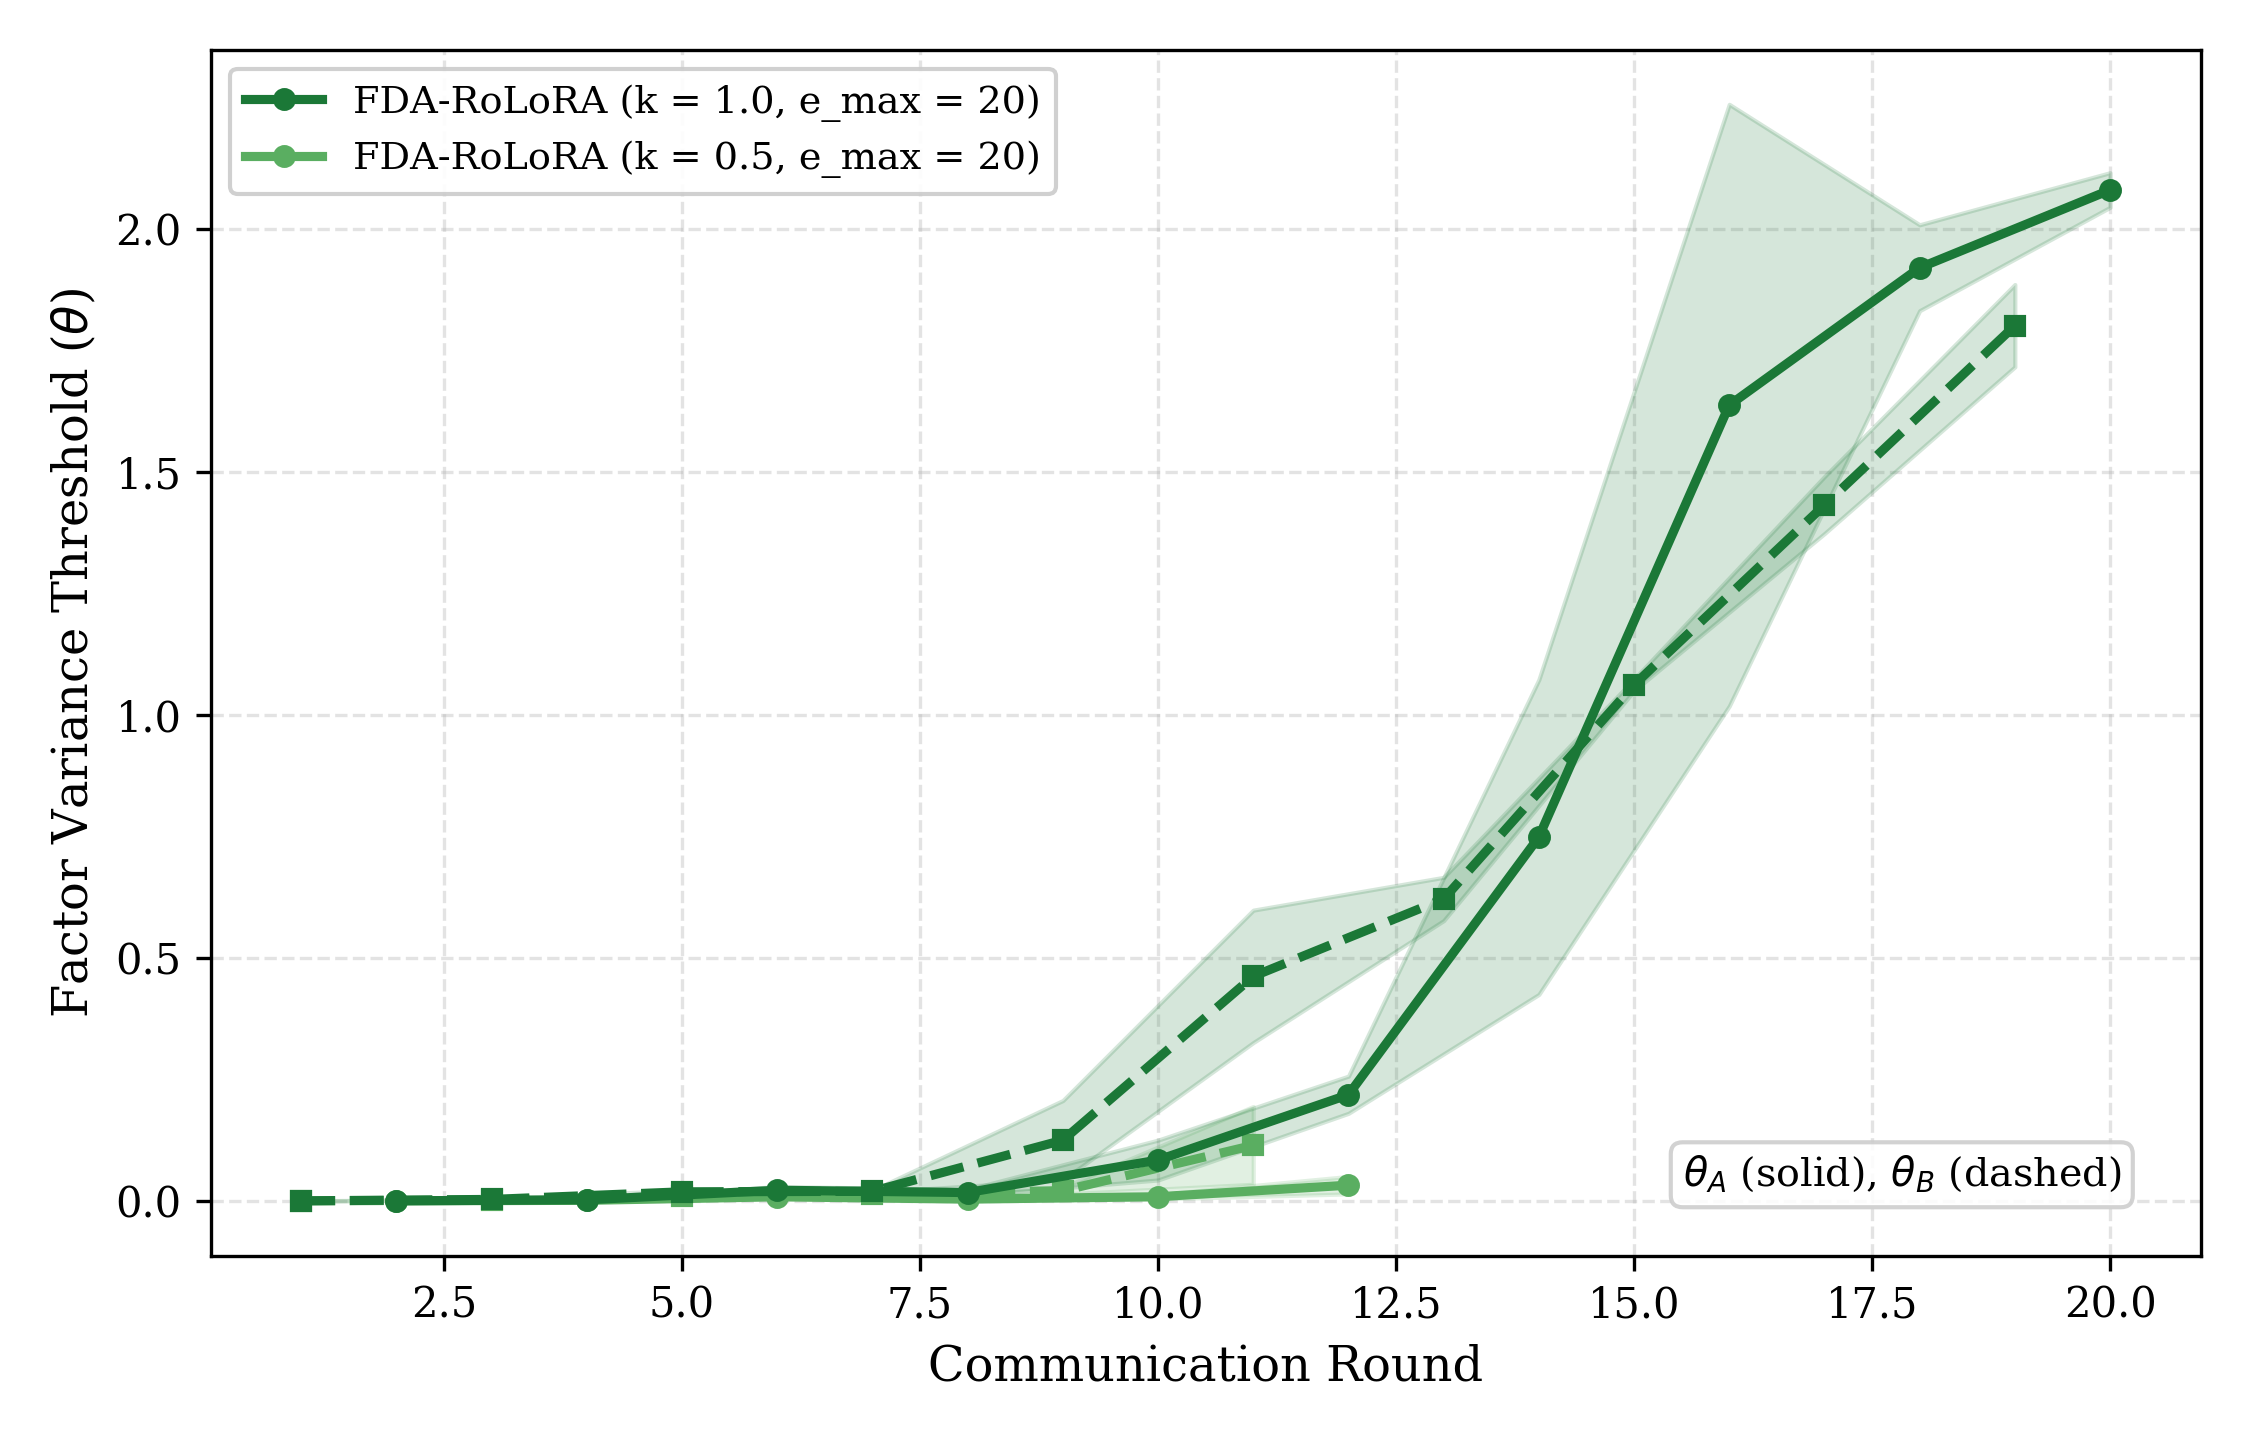
\includegraphics[width=\textwidth,height=4.9cm,keepaspectratio]{figures/telemetry/11_SST2_C20_R50_LR0.1_5_fda_threshold.png}
            \vspace{2pt}
            \par{\footnotesize \textbf{(d)} Factor Thresholds ($\theta_A, \theta_B$)}
        \end{minipage}

        \vspace{0.6em}
        \begin{minipage}[b]{0.485\textwidth}
            \centering
            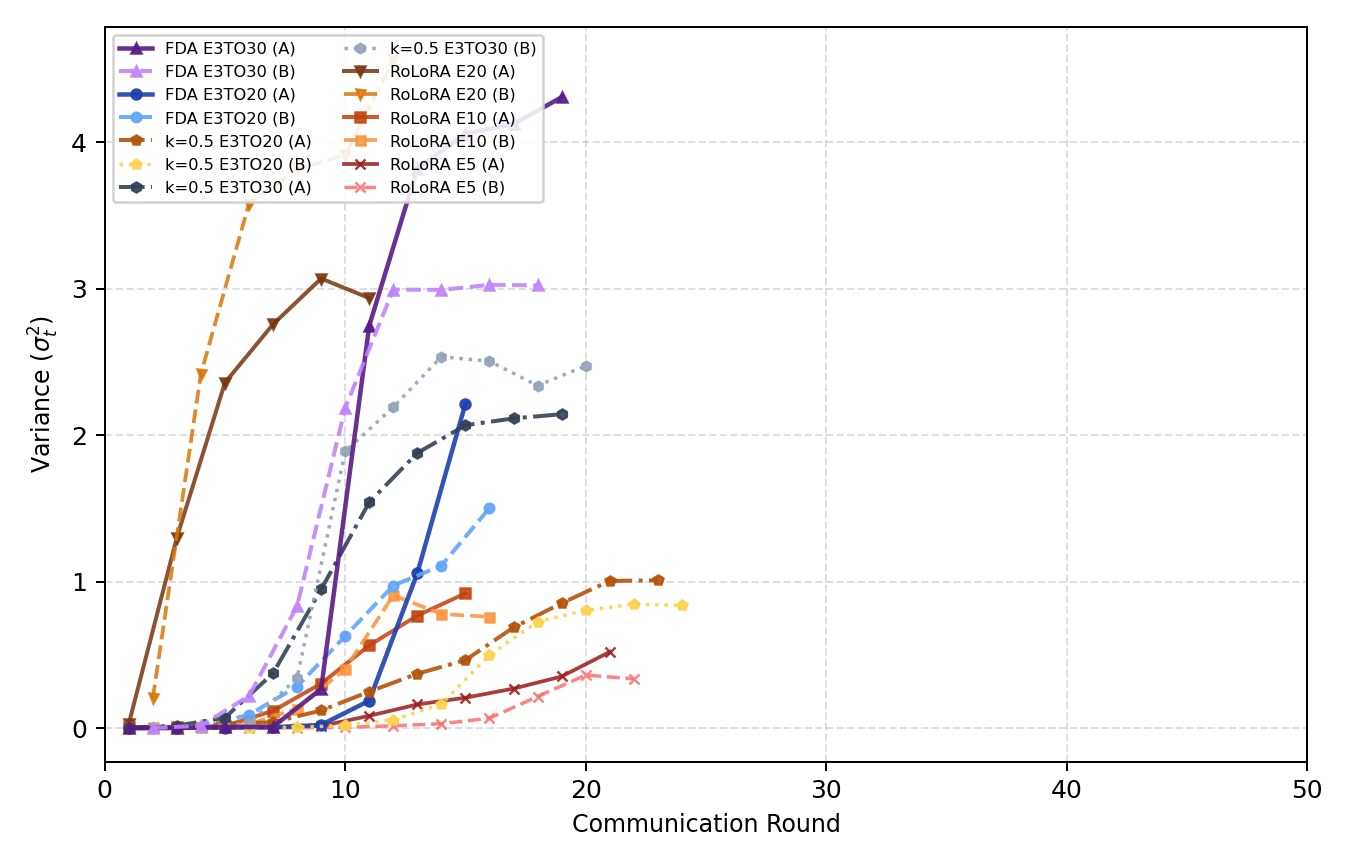
\includegraphics[width=\textwidth,height=4.9cm,keepaspectratio]{figures/telemetry/11_SST2_C20_R50_LR0.1_3_client_variance.png}
            \vspace{2pt}
            \par{\footnotesize \textbf{(e)} Subspace Coordinate Variance}
        \end{minipage}\hfill
        \begin{minipage}[b]{0.485\textwidth}
            \centering
            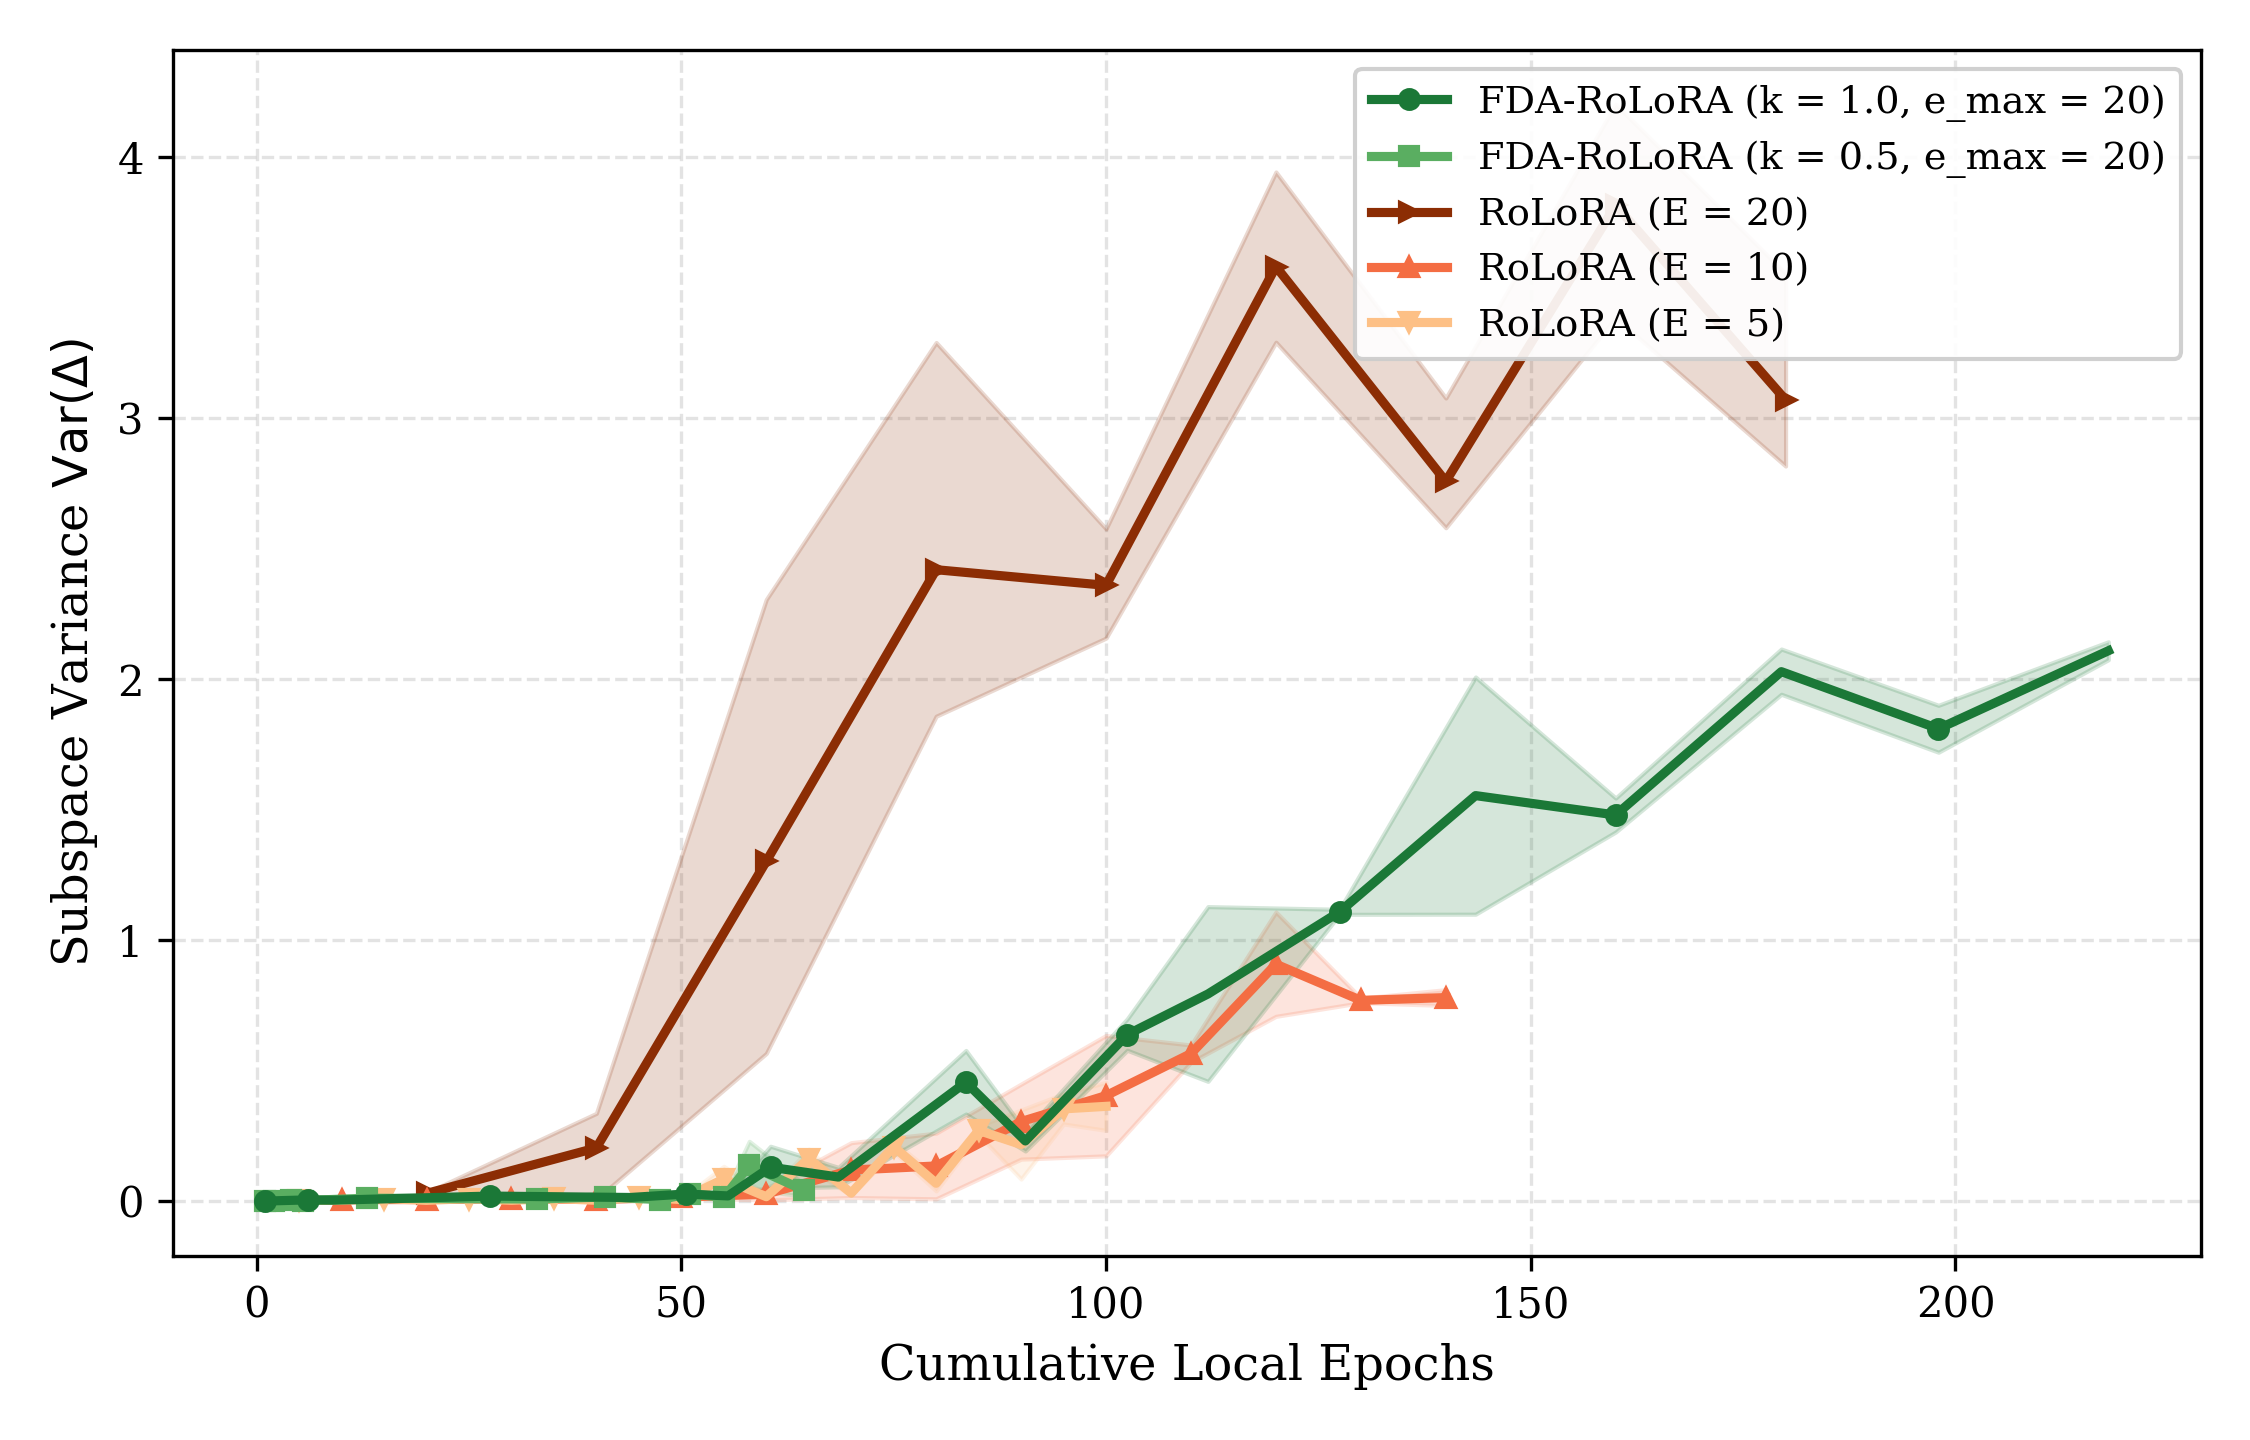
\includegraphics[width=\textwidth,height=4.9cm,keepaspectratio]{figures/telemetry/11_SST2_C20_R50_LR0.1_6_variance_vs_epoch.png}
            \vspace{2pt}
            \par{\footnotesize \textbf{(f)} Variance vs.\ Cumulative Local Epochs}
        \end{minipage}

        \vspace{0.6em}
        \caption{Multi-panel optimization telemetry on SST-2 ($C=20, R_{\max}=50, \eta_c=0.1, \alpha=1000.0$) comparing FDA-RoLoRA against static RoLoRA baselines under homogeneous consensus.}
        \label{fig:telemetry_sst2_c20_iid}
    \end{minipage}%
    }
\end{figure}

\begin{figure}[p]
    \centering
    \makebox[\textwidth][c]{%
    \begin{minipage}{1.06\textwidth}
        \begin{minipage}[b]{0.485\textwidth}
            \centering
            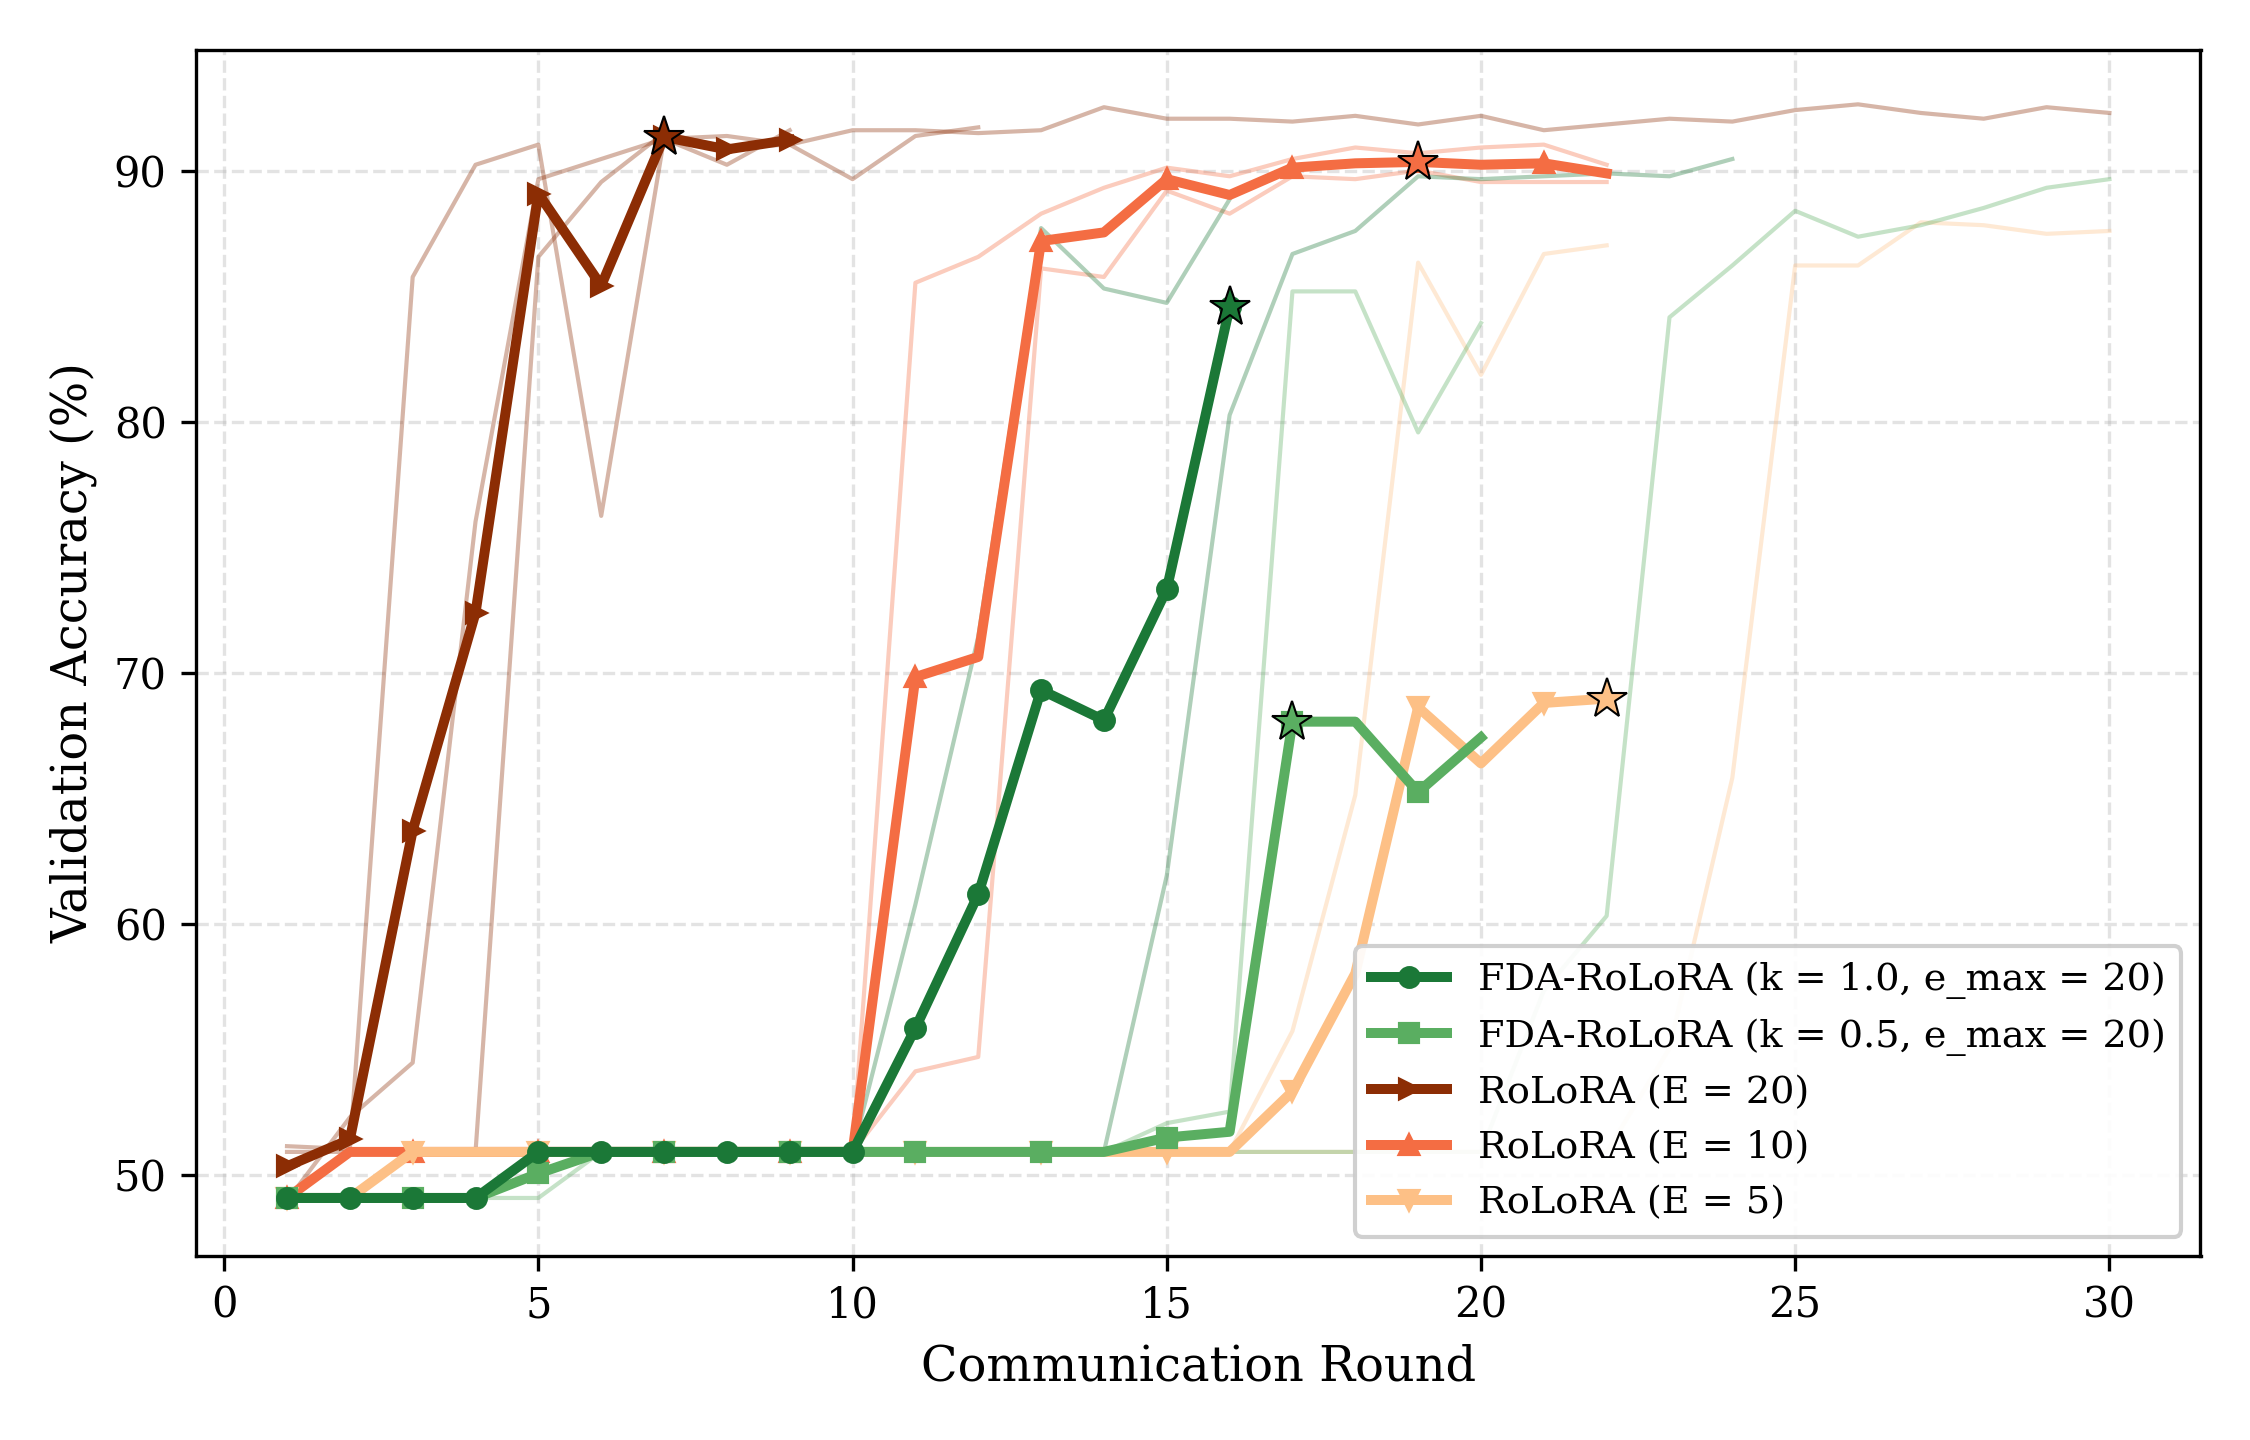
\includegraphics[width=\textwidth,height=4.9cm,keepaspectratio]{figures/telemetry/12_SST2_C50_R30_LR0.1_1_accuracy.png}
            \vspace{2pt}
            \par{\footnotesize \textbf{(a)} Validation Accuracy}
        \end{minipage}\hfill
        \begin{minipage}[b]{0.485\textwidth}
            \centering
            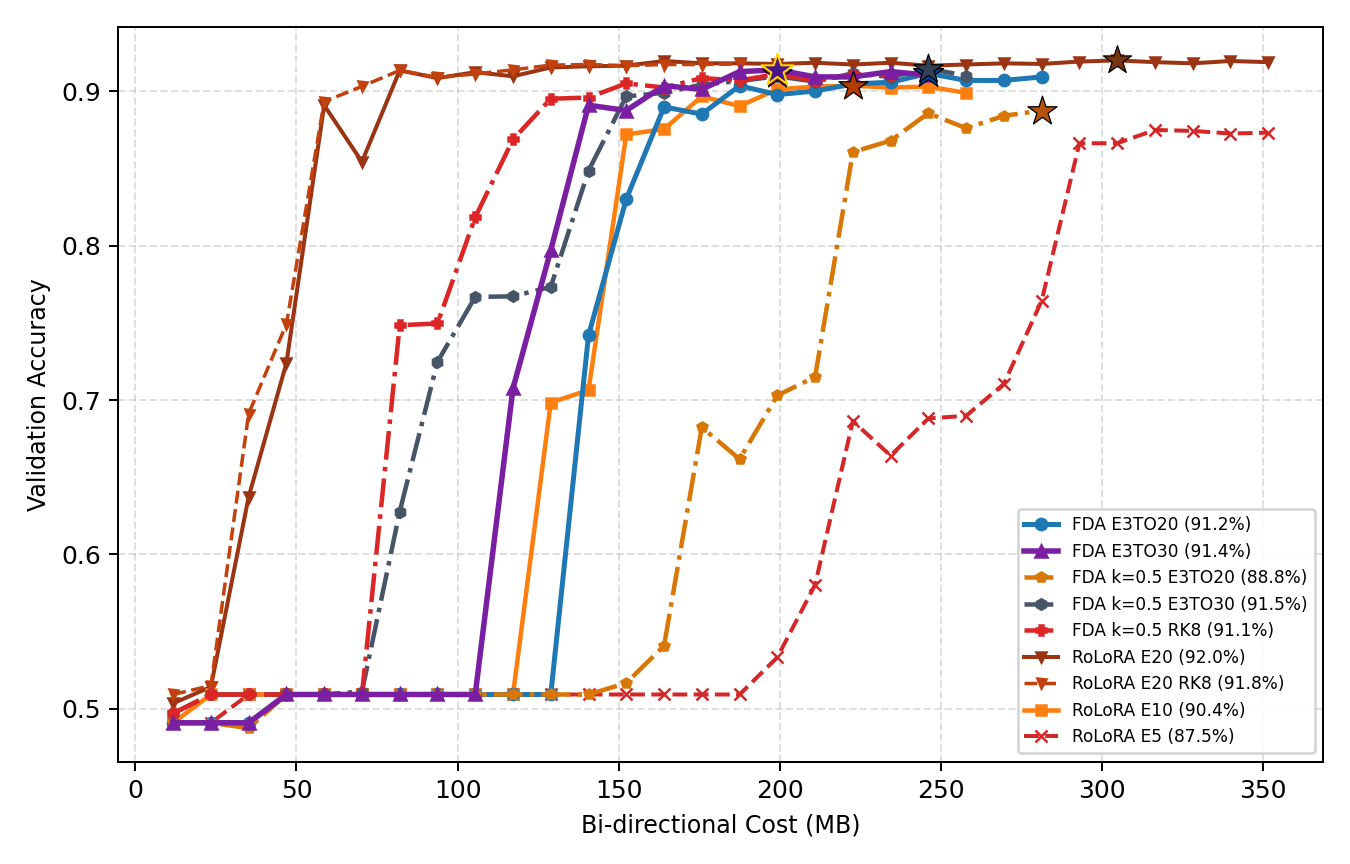
\includegraphics[width=\textwidth,height=4.9cm,keepaspectratio]{figures/telemetry/12_SST2_C50_R30_LR0.1_4_accuracy_vs_cost.png}
            \vspace{2pt}
            \par{\footnotesize \textbf{(b)} Accuracy vs. Communication (MB)}
        \end{minipage}

        \vspace{0.6em}
        \begin{minipage}[b]{0.485\textwidth}
            \centering
            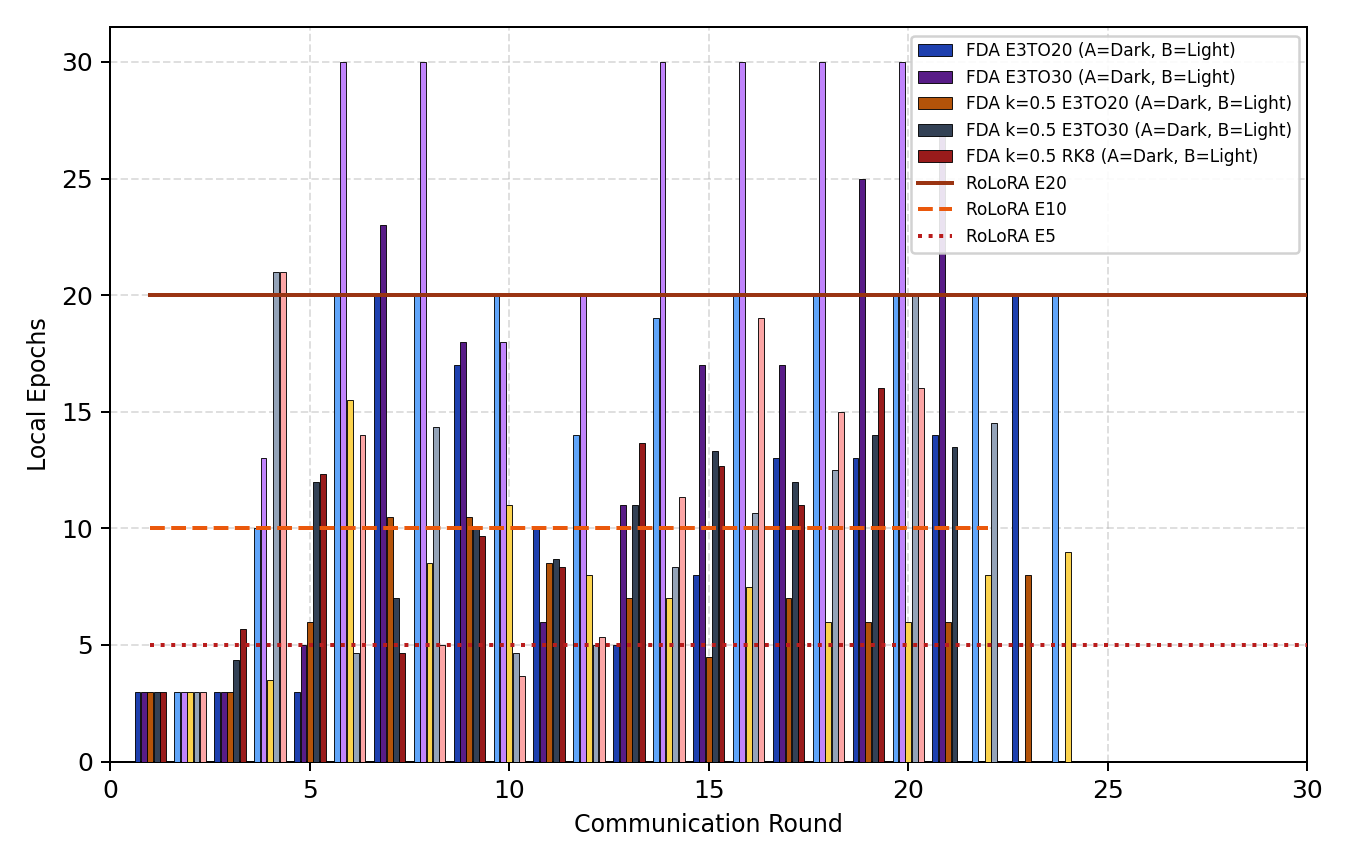
\includegraphics[width=\textwidth,height=4.9cm,keepaspectratio]{figures/telemetry/12_SST2_C50_R30_LR0.1_2_allocated_epochs.png}
            \vspace{2pt}
            \par{\footnotesize \textbf{(c)} Dynamic Local Epochs ($\bar{e}$)}
        \end{minipage}\hfill
        \begin{minipage}[b]{0.485\textwidth}
            \centering
            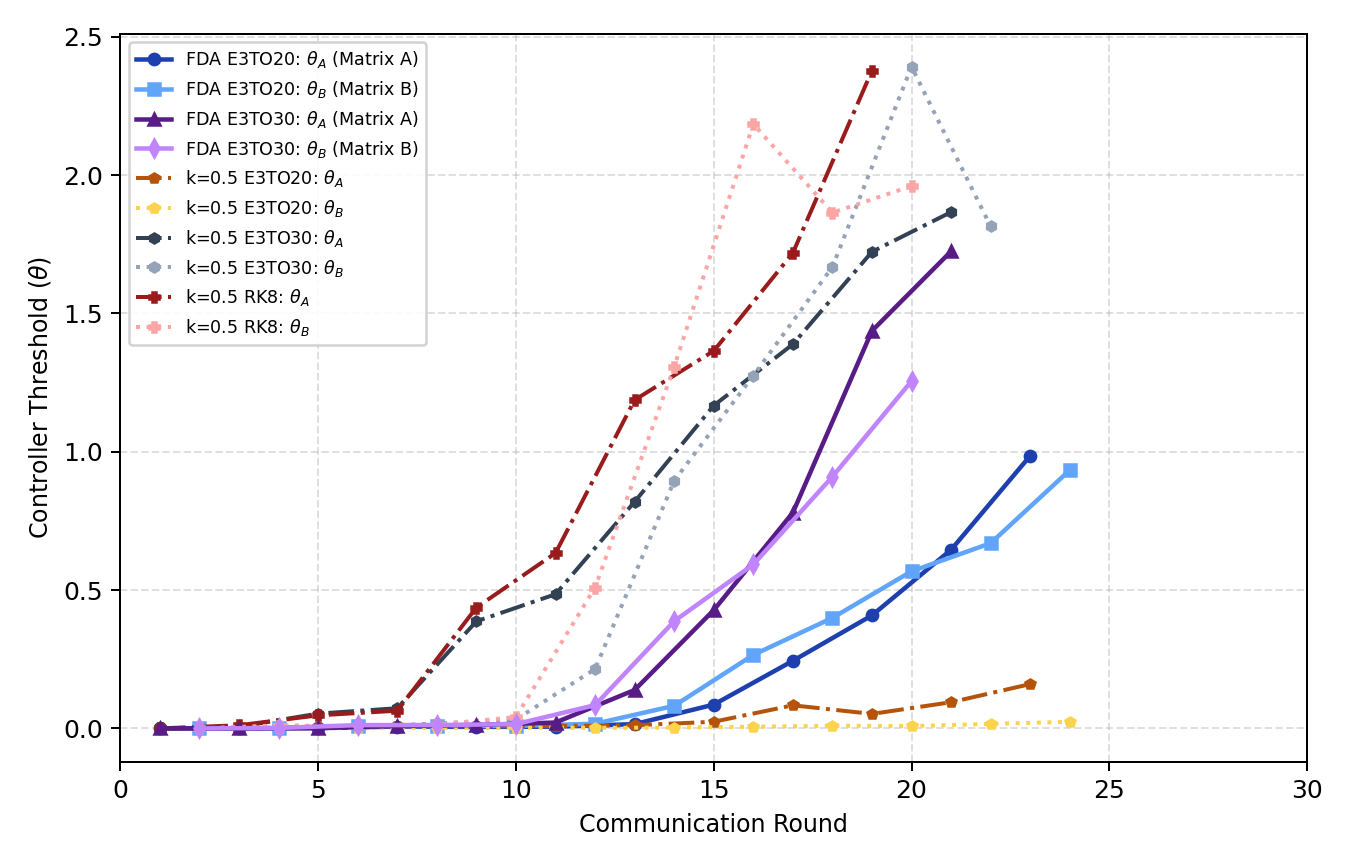
\includegraphics[width=\textwidth,height=4.9cm,keepaspectratio]{figures/telemetry/12_SST2_C50_R30_LR0.1_5_fda_threshold.png}
            \vspace{2pt}
            \par{\footnotesize \textbf{(d)} Factor Thresholds ($\theta_A, \theta_B$)}
        \end{minipage}

        \vspace{0.6em}
        \begin{minipage}[b]{0.485\textwidth}
            \centering
            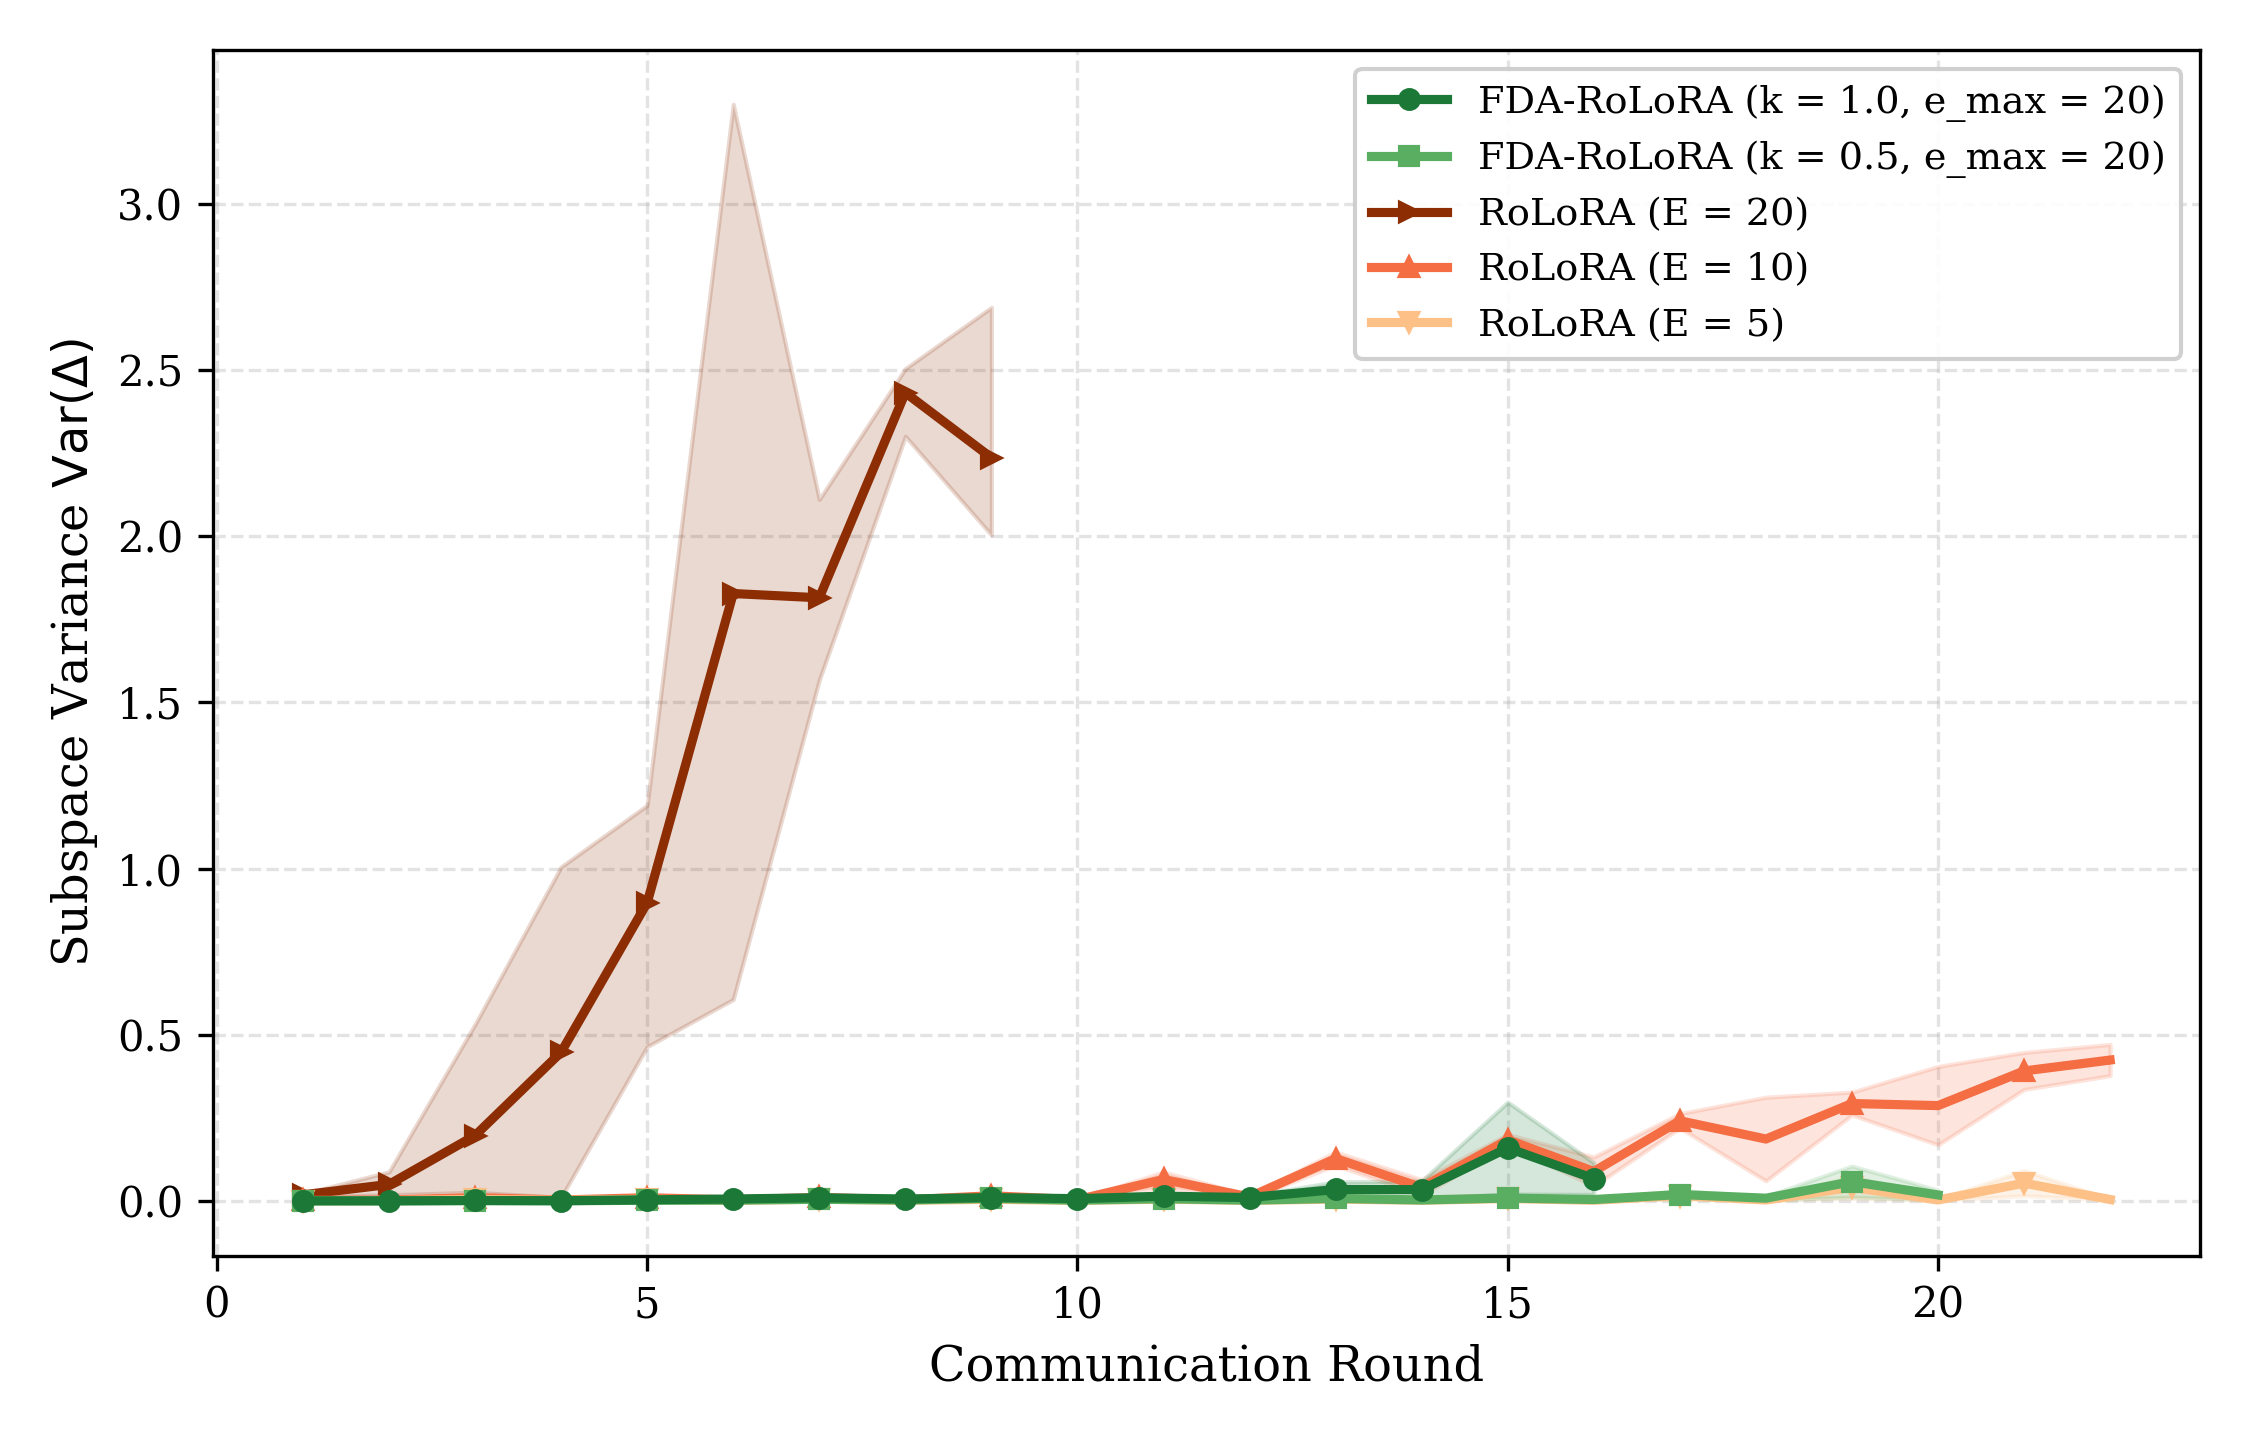
\includegraphics[width=\textwidth,height=4.9cm,keepaspectratio]{figures/telemetry/12_SST2_C50_R30_LR0.1_3_client_variance.png}
            \vspace{2pt}
            \par{\footnotesize \textbf{(e)} Subspace Coordinate Variance}
        \end{minipage}\hfill
        \begin{minipage}[b]{0.485\textwidth}
            \centering
            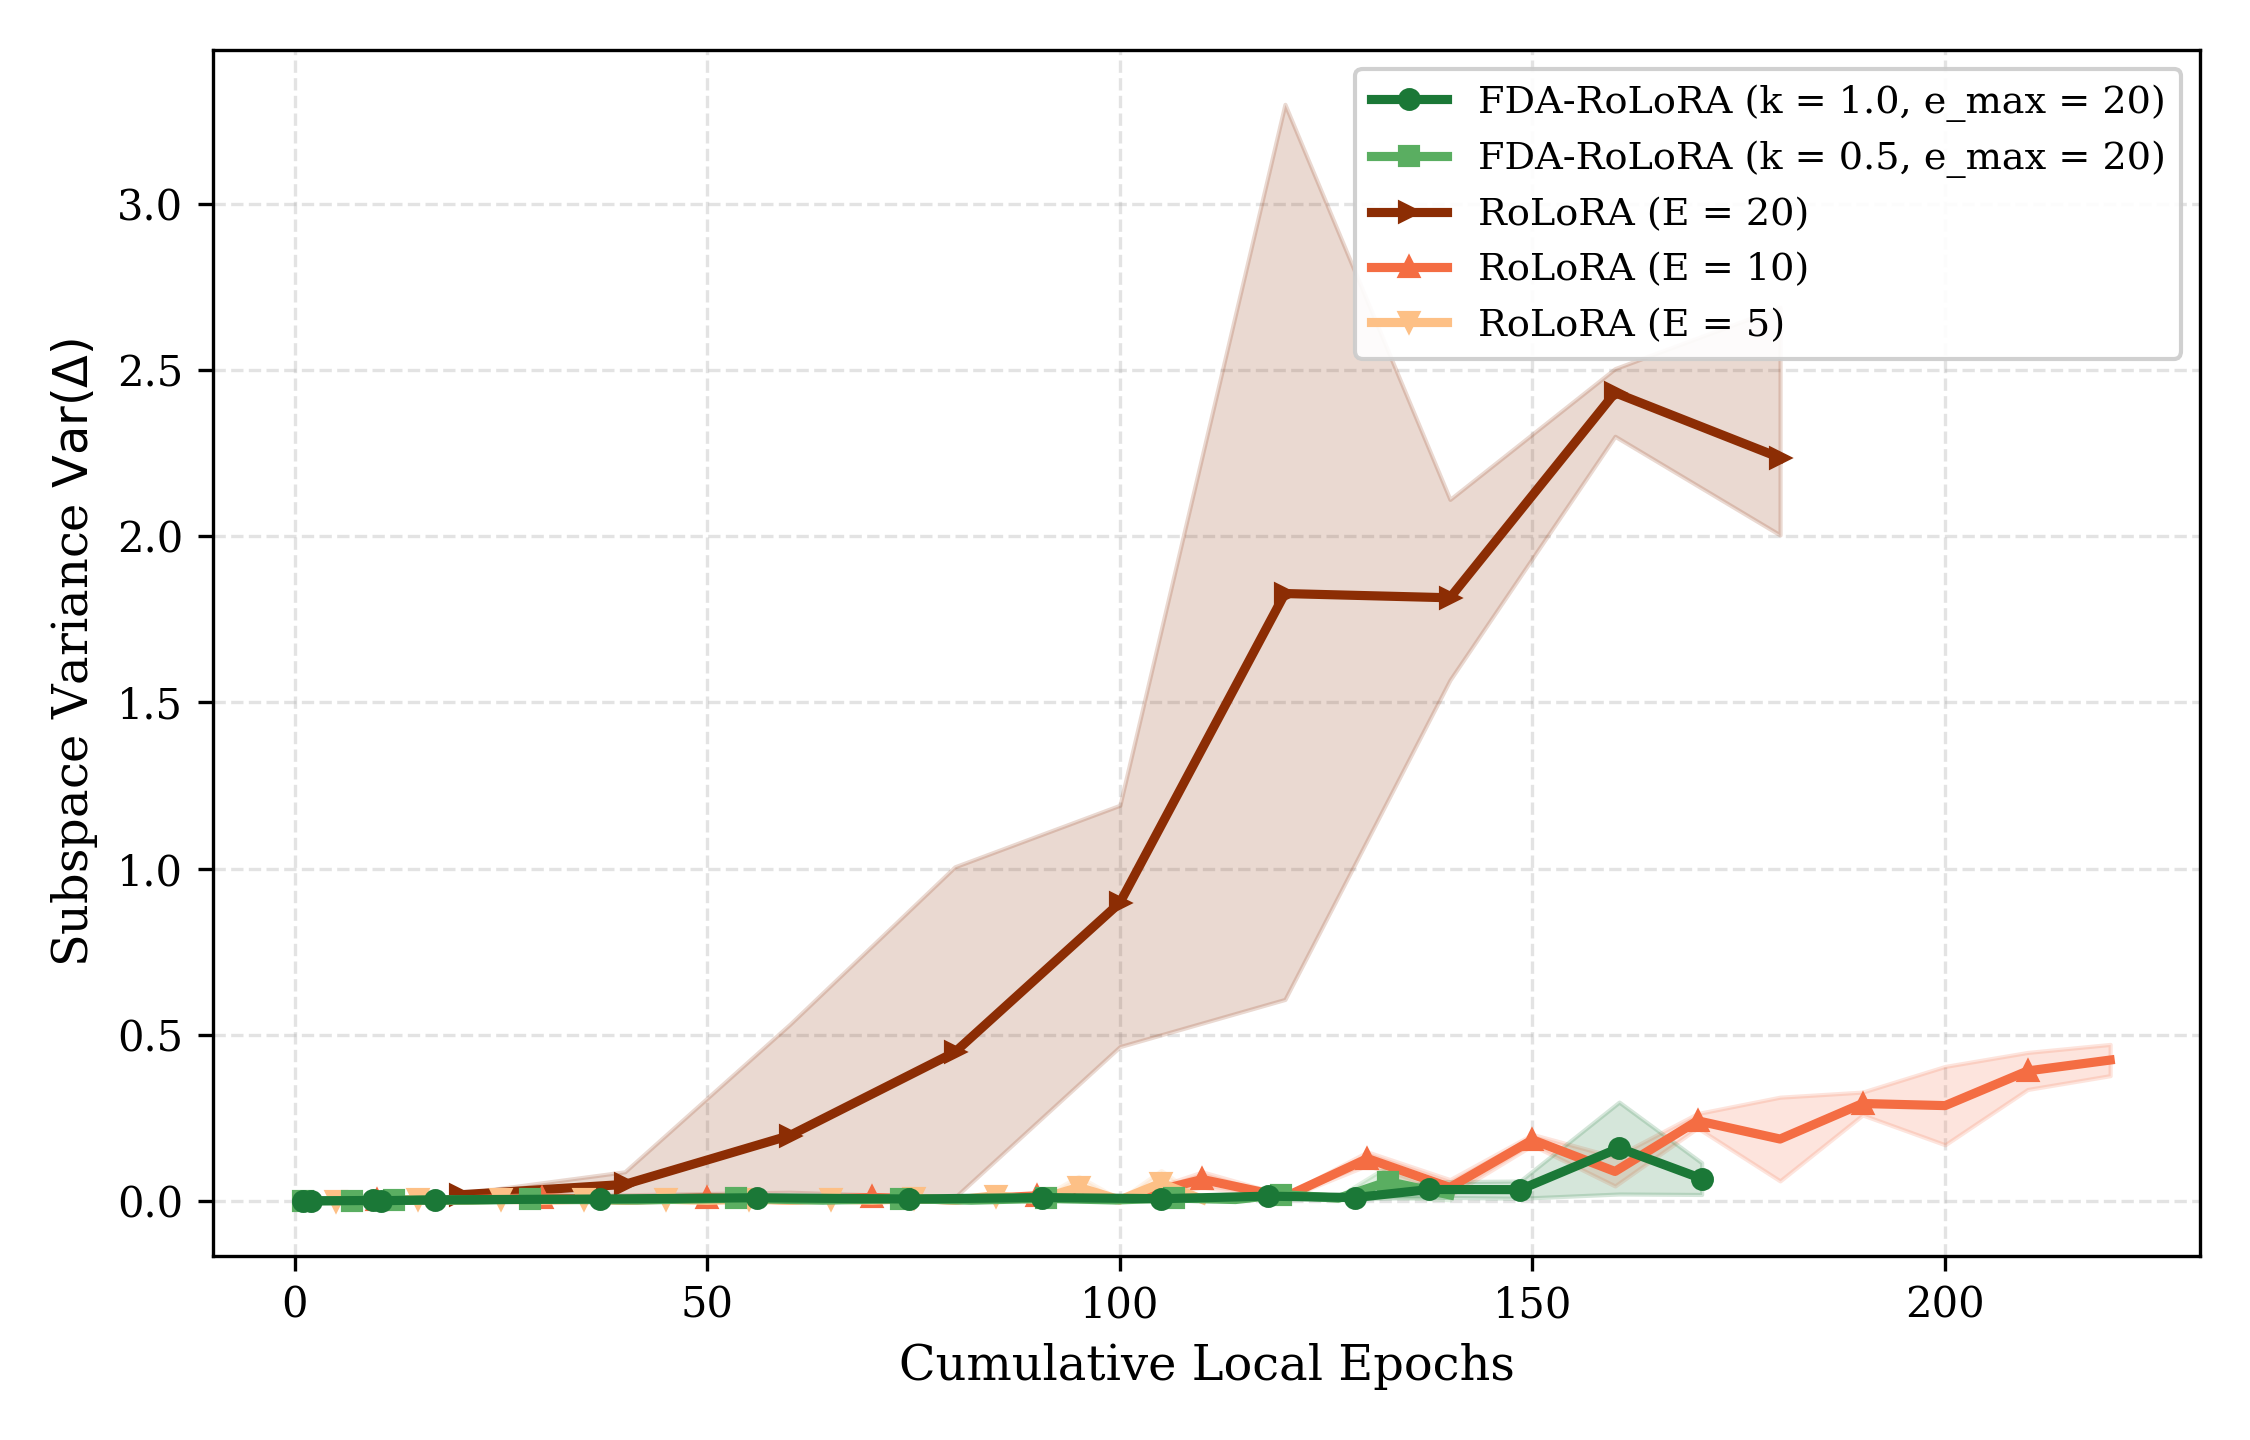
\includegraphics[width=\textwidth,height=4.9cm,keepaspectratio]{figures/telemetry/12_SST2_C50_R30_LR0.1_6_variance_vs_epoch.png}
            \vspace{2pt}
            \par{\footnotesize \textbf{(f)} Variance vs.\ Cumulative Local Epochs}
        \end{minipage}

        \vspace{0.6em}
        \caption{Multi-panel optimization telemetry on SST-2 ($C=50, R_{\max}=30, \eta_c=0.1, \alpha=1000.0$) under expanded cohort scale $C=50$.}
        \label{fig:telemetry_sst2_c50_iid}
    \end{minipage}%
    }
\end{figure}

\clearpage

% ==============================================================================
% SECTION 5.3: BENCHMARK SUITE 2: STATISTICAL HETEROGENEITY
% ==============================================================================
\section{Benchmark Suite 2: Statistical Heterogeneity}
\label{sec:eval_non_iid}

While homogeneous settings demonstrate baseline efficiency, practical federated networks are defined by severe statistical data heterogeneity. To rigorously evaluate the closed-loop resilience of our framework under real-world stress, we investigate severe non-IID conditions modeled via Dirichlet label distribution skew with concentration parameter $\alpha = 0.5$. Adopting $\alpha = 0.5$ directly follows the non-IID benchmarking protocol of RoLoRA~\cite{chen2025robust} and established federated learning literature~\cite{hsu2019measuring, zhu2021federated}, representing an acute label distribution skew where individual clients hold heavily biased class proportions.

Table~\ref{tab:non_iid_detailed_benchmarks} compiles the complete empirical evaluation across all four GLUE sequence classification benchmarks under Dirichlet label skew ($\alpha=0.5$). The table presents all evaluated fixed-budget RoLoRA baselines alongside FDA-RoLoRA across controller horizon ratios $k \in \{0.5, 1.0\}$ and extended horizons ($e_{\max}=40$), explicitly reporting factor-decomposed local epoch allocations ($\bar{e}_A$ and $\bar{e}_B$).

% Auto-generated by FDA-RoLoRA analysis/thesis_final_audit/generate_thesis_tables.py
% Based on code repo commit: 1c2bf55
% Strict data integrity audit: per-seed metrics from raw CSVs in results/round_metrics/
% Do not edit manually.

\begin{table}[htbp]
\centering
\small
\resizebox{\textwidth}{!}{
\begin{tabular}{|l|l|l|c|c|c|c|c|c|c|}
\hline
\textbf{Task} & \textbf{Cohort} & \textbf{Methodology} & \textbf{Final Acc. (\%)} & \textbf{Peak Acc. (\%)} & \textbf{Rounds ($R$)} & \textbf{Total MB} & \textbf{Mean $\bar{e}$} & \textbf{Mean $\bar{e}_A$} & \textbf{Mean $\bar{e}_B$} \\
\hline
\multirow{8}{*}{\textbf{MNLI}} 
& \multirow{5}{*}{$C=20$} 
& FDA-RoLoRA E1TO40 (k=0.5) & $73.70 \pm 0.34$ & $74.12 \pm 0.93$ & $34.5 \pm 0.7$ & $161.7\,\text{MB}$ & $19.06$ & $18.82$ & $19.29$ \\
& & FDA-RoLoRA E1TO20 (k=0.5) & $72.48 \pm 0.14$ & $73.25 \pm 1.19$ & $41.0 \pm 7.1$ & $192.2\,\text{MB}$ & $10.07$ & $9.96$ & $10.18$ \\
& & FDA-RoLoRA E1TO20 (k=1.0) & $73.71 \pm 0.77$ & $\mathbf{74.47 \pm 0.11}$ & $38.0 \pm 4.2$ & $178.1\,\text{MB}$ & $17.49$ & $17.19$ & $17.76$ \\
& & RoLoRA E20 & $68.87 \pm 6.46$ & $73.31 \pm 0.18$ & $\mathbf{24.0 \pm 5.7}$ & $\mathbf{112.5\,\text{MB}}$ & $20.00$ & $20.00$ & $20.00$ \\
& & RoLoRA E10 & $\mathbf{74.11 \pm 0.31}$ & $74.24 \pm 0.12$ & $50.0$ & $234.4\,\text{MB}$ & $10.00$ & $10.00$ & $10.00$ \\
\cline{2-10}
& \multirow{3}{*}{$C=50$} 
& FDA-RoLoRA E1TO20 (k=1.0) & $51.46 \pm 8.46$ & $54.95 \pm 3.53$ & $\mathbf{22.5 \pm 2.1}$ & $\mathbf{263.7\,\text{MB}}$ & $15.63$ & $15.03$ & $16.20$ \\
& & FDA-RoLoRA E1TO20 (k=0.5) & $55.23 \pm 2.11$ & $55.56 \pm 1.65$ & $30.0$ & $351.6\,\text{MB}$ & $10.13$ & $9.47$ & $10.80$ \\
& & RoLoRA E10 & $\mathbf{56.22 \pm 7.40}$ & $\mathbf{56.55 \pm 6.94}$ & $30.0$ & $351.6\,\text{MB}$ & $10.00$ & $10.00$ & $10.00$ \\
\hline
\multirow{9}{*}{\textbf{QNLI}} 
& \multirow{6}{*}{$C=20$} 
& FDA-RoLoRA E1TO40 (k=1.0) & $76.27 \pm 7.78$ & $83.20 \pm 0.18$ & $\mathbf{15.0 \pm 4.2}$ & $\mathbf{70.3\,\text{MB}}$ & $29.83$ & $30.14$ & $29.53$ \\
& & FDA-RoLoRA E1TO40 (k=0.5) & $79.12 \pm 6.72$ & $83.48 \pm 0.94$ & $24.0 \pm 8.5$ & $112.5\,\text{MB}$ & $20.36$ & $21.24$ & $19.47$ \\
& & FDA-RoLoRA E1TO20 (k=1.0) & $81.88 \pm 2.90$ & $\mathbf{84.22 \pm 0.41}$ & $26.5 \pm 7.8$ & $124.2\,\text{MB}$ & $16.73$ & $16.63$ & $16.81$ \\
& & FDA-RoLoRA E1TO20 (k=0.5) & $74.03 \pm 13.98$ & $82.64 \pm 2.63$ & $34.0 \pm 5.7$ & $159.4\,\text{MB}$ & $10.54$ & $10.81$ & $10.27$ \\
& & RoLoRA E20 & $\mathbf{82.97 \pm 0.50}$ & $83.22 \pm 0.14$ & $19.0 \pm 2.8$ & $89.1\,\text{MB}$ & $20.00$ & $20.00$ & $20.00$ \\
& & RoLoRA E10 & $81.10 \pm 4.31$ & $83.50 \pm 1.67$ & $33.0 \pm 1.4$ & $154.7\,\text{MB}$ & $10.00$ & $10.00$ & $10.00$ \\
\cline{2-10}
& \multirow{3}{*}{$C=50$} 
& FDA-RoLoRA E1TO20 (k=1.0) & $49.51 \pm 0.08$ & $73.52 \pm 4.31$ & $\mathbf{13.0}$ & $\mathbf{152.3\,\text{MB}}$ & $13.04$ & $13.17$ & $12.93$ \\
& & FDA-RoLoRA E1TO20 (k=0.5) & $50.13 \pm 0.94$ & $\mathbf{75.69 \pm 1.66}$ & $30.0$ & $351.6\,\text{MB}$ & $10.48$ & $9.83$ & $11.13$ \\
& & RoLoRA E10 & $\mathbf{58.45 \pm 12.71}$ & $74.61 \pm 10.15$ & $30.0$ & $351.6\,\text{MB}$ & $10.00$ & $10.00$ & $10.00$ \\
\hline
\multirow{6}{*}{\textbf{QQP}} 
& \multirow{3}{*}{$C=20$} 
& FDA-RoLoRA E1TO20 (k=1.0) & $64.52 \pm 18.23$ & $\mathbf{77.88 \pm 0.66}$ & $14.0 \pm 2.8$ & $65.6\,\text{MB}$ & $15.70$ & $15.77$ & $15.62$ \\
& & FDA-RoLoRA E1TO20 (k=0.5) & $48.32 \pm 12.63$ & $73.58 \pm 1.56$ & $\mathbf{12.0 \pm 4.2}$ & $\mathbf{56.2\,\text{MB}}$ & $10.87$ & $11.79$ & $10.10$ \\
& & RoLoRA E10 & $\mathbf{76.76 \pm 3.41}$ & $77.69 \pm 2.18$ & $16.5 \pm 0.7$ & $77.3\,\text{MB}$ & $10.00$ & $10.00$ & $10.00$ \\
\cline{2-10}
& \multirow{3}{*}{$C=50$} 
& FDA-RoLoRA E1TO20 (k=1.0) & $57.45 \pm 11.29$ & $74.55 \pm 1.30$ & $\mathbf{15.5 \pm 3.5}$ & $\mathbf{181.6\,\text{MB}}$ & $14.26$ & $13.83$ & $14.63$ \\
& & FDA-RoLoRA E1TO20 (k=0.5) & $53.46 \pm 19.74$ & $72.71 \pm 3.23$ & $\mathbf{15.5 \pm 4.9}$ & $\mathbf{181.6\,\text{MB}}$ & $9.18$ & $8.89$ & $9.48$ \\
& & RoLoRA E10 & $\mathbf{69.28 \pm 8.14}$ & $\mathbf{74.71 \pm 1.63}$ & $22.5 \pm 2.1$ & $263.7\,\text{MB}$ & $10.00$ & $10.00$ & $10.00$ \\
\hline
\multirow{6}{*}{\textbf{SST-2}} 
& \multirow{3}{*}{$C=20$} 
& FDA-RoLoRA E1TO20 (k=1.0) & $69.72 \pm 29.19$ & $\mathbf{89.91 \pm 0.81}$ & $\mathbf{14.0}$ & $\mathbf{39.4\,\text{MB}}$ & $14.43$ & $14.57$ & $14.29$ \\
& & FDA-RoLoRA E1TO20 (k=0.5) & $79.36 \pm 16.38$ & $89.39 \pm 2.19$ & $16.0 \pm 2.8$ & $45.0\,\text{MB}$ & $9.69$ & $10.32$ & $9.06$ \\
& & RoLoRA E10 & $\mathbf{89.62 \pm 1.87}$ & $89.62 \pm 1.87$ & $25.0$ & $70.3\,\text{MB}$ & $10.00$ & $10.00$ & $10.00$ \\
\cline{2-10}
& \multirow{3}{*}{$C=50$} 
& FDA-RoLoRA E1TO20 (k=1.0) & $\mathbf{81.36 \pm 9.97}$ & $\mathbf{85.95 \pm 5.60}$ & $\mathbf{20.0}$ & $\mathbf{140.6\,\text{MB}}$ & $14.57$ & $14.60$ & $14.55$ \\
& & FDA-RoLoRA E1TO20 (k=0.5) & $66.46 \pm 24.57$ & $67.37 \pm 23.27$ & $\mathbf{20.0}$ & $\mathbf{140.6\,\text{MB}}$ & $8.70$ & $8.40$ & $9.00$ \\
& & RoLoRA E10 & $53.33 \pm 3.08$ & $59.00 \pm 11.11$ & $\mathbf{20.0}$ & $\mathbf{140.6\,\text{MB}}$ & $10.00$ & $10.00$ & $10.00$ \\
\hline
\end{tabular}
}
\caption{Detailed Telemetry Across All Non-IID Configurations ($\alpha=0.5$): RoLoRA vs.\ FDA-RoLoRA across GLUE benchmarks under Dirichlet label skew.}
\label{tab:non_iid_detailed_benchmarks}
\end{table}

\paragraph{MNLI: Asymmetric Factor Allocation \& Post-Peak Collapse.}
On 3-class sentence-pair inference under acute Dirichlet label skew ($\alpha=0.5, C=20, R_{\max}=50$), Figure~\ref{fig:telemetry_mnli_non_iid} illustrates optimization dynamics across all six telemetry panels. Under static schedules ($E=20$), forcing clients through unconstrained local training drives updates into conflicting subspaces: validation accuracy (Panel a) peaks early at $73.31\%$ and then suffers catastrophic post-peak collapse down to $68.09\%$. In contrast, FDA-RoLoRA ($k=1.0$) dynamically monitors coordinate variance, achieving a superior peak accuracy of $\mathbf{74.47\%}$ and stopping after 41 and 35 rounds (seeds 42 and 43) at final accuracies of $73.17\%$ and $74.25\%$. At those same rounds, RoLoRA $E=10$ had reached only $70.23\%$ and $71.86\%$, and it needed 47 and 50 rounds to match FDA-RoLoRA's final accuracy. FDA-RoLoRA therefore reaches the same accuracy in roughly 15--30\% fewer rounds ($178.1\,\text{MB}$ vs.\ $234.4\,\text{MB}$ on average), while executing about $1.75\times$ more local epochs per round ($\bar{e}=17.49$ vs.\ 10). 

Crucially, local epoch telemetry (Panel c) and decoupled threshold trajectories (Panel d) reveal the mechanistic basis of this stability: factor matrix $B$ safely accommodates deeper local training ($\bar{e}_B = 17.76$) under an expanded threshold $\theta_B$, whereas down-projection factor $A$ encounters sharper gradient drift, prompting threshold $\theta_A$ to enforce earlier synchronization ($\bar{e}_A = 17.19$). Subspace coordinate variance (Panel e) surges by over $2\times$ compared to IID regimes ($\bar{\nu} \approx 6.5\text{--}8.0$), reflecting severe inter-client gradient conflict.
\begin{figure}[p]
    \centering
    \makebox[\textwidth][c]{%
    \begin{minipage}{1.06\textwidth}
        \begin{minipage}[b]{0.485\textwidth}
            \centering
            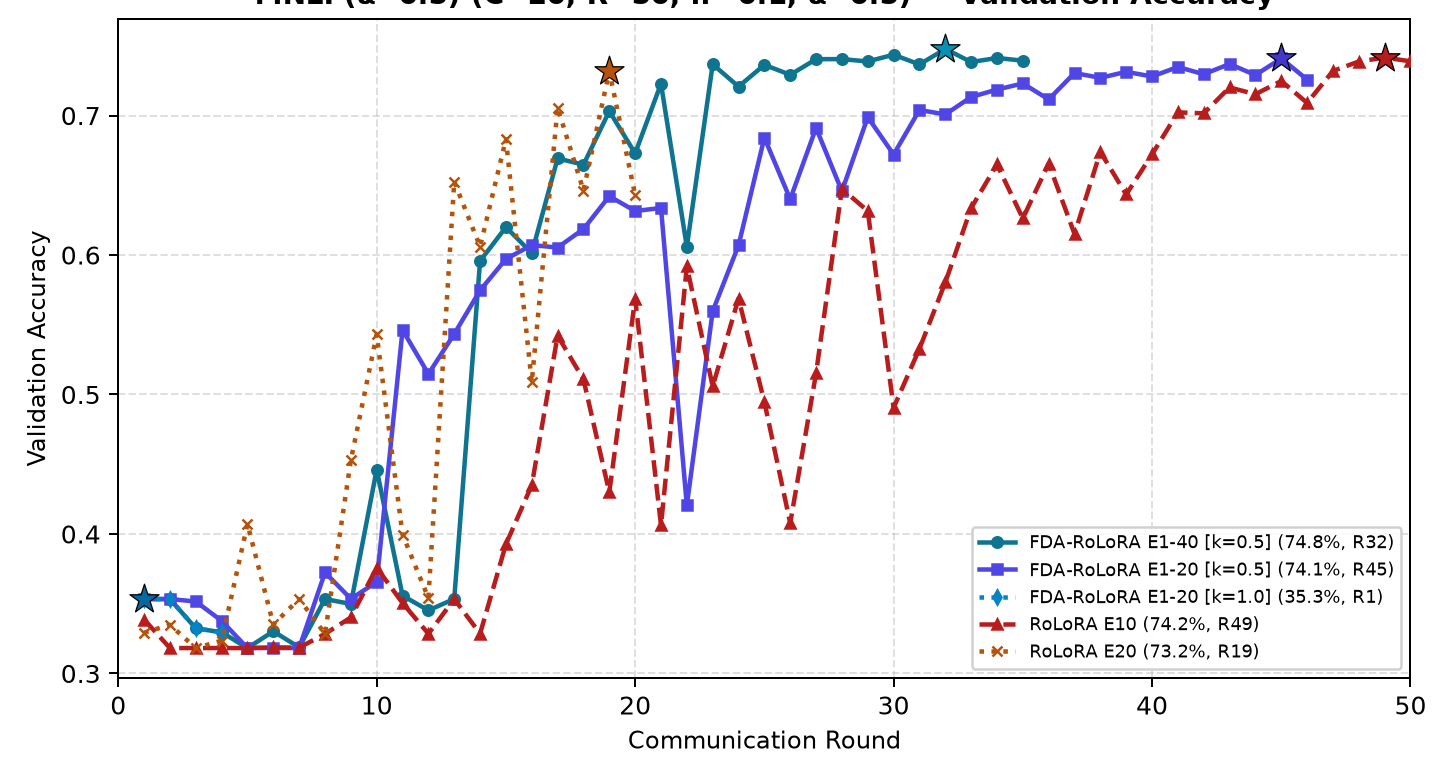
\includegraphics[width=\textwidth,height=4.9cm,keepaspectratio]{figures/telemetry/17_MNLI_C20_R50_LR0.1_A0.5_1_accuracy.png}
            \vspace{2pt}
            \par{\footnotesize \textbf{(a)} Validation Accuracy}
        \end{minipage}\hfill
        \begin{minipage}[b]{0.485\textwidth}
            \centering
            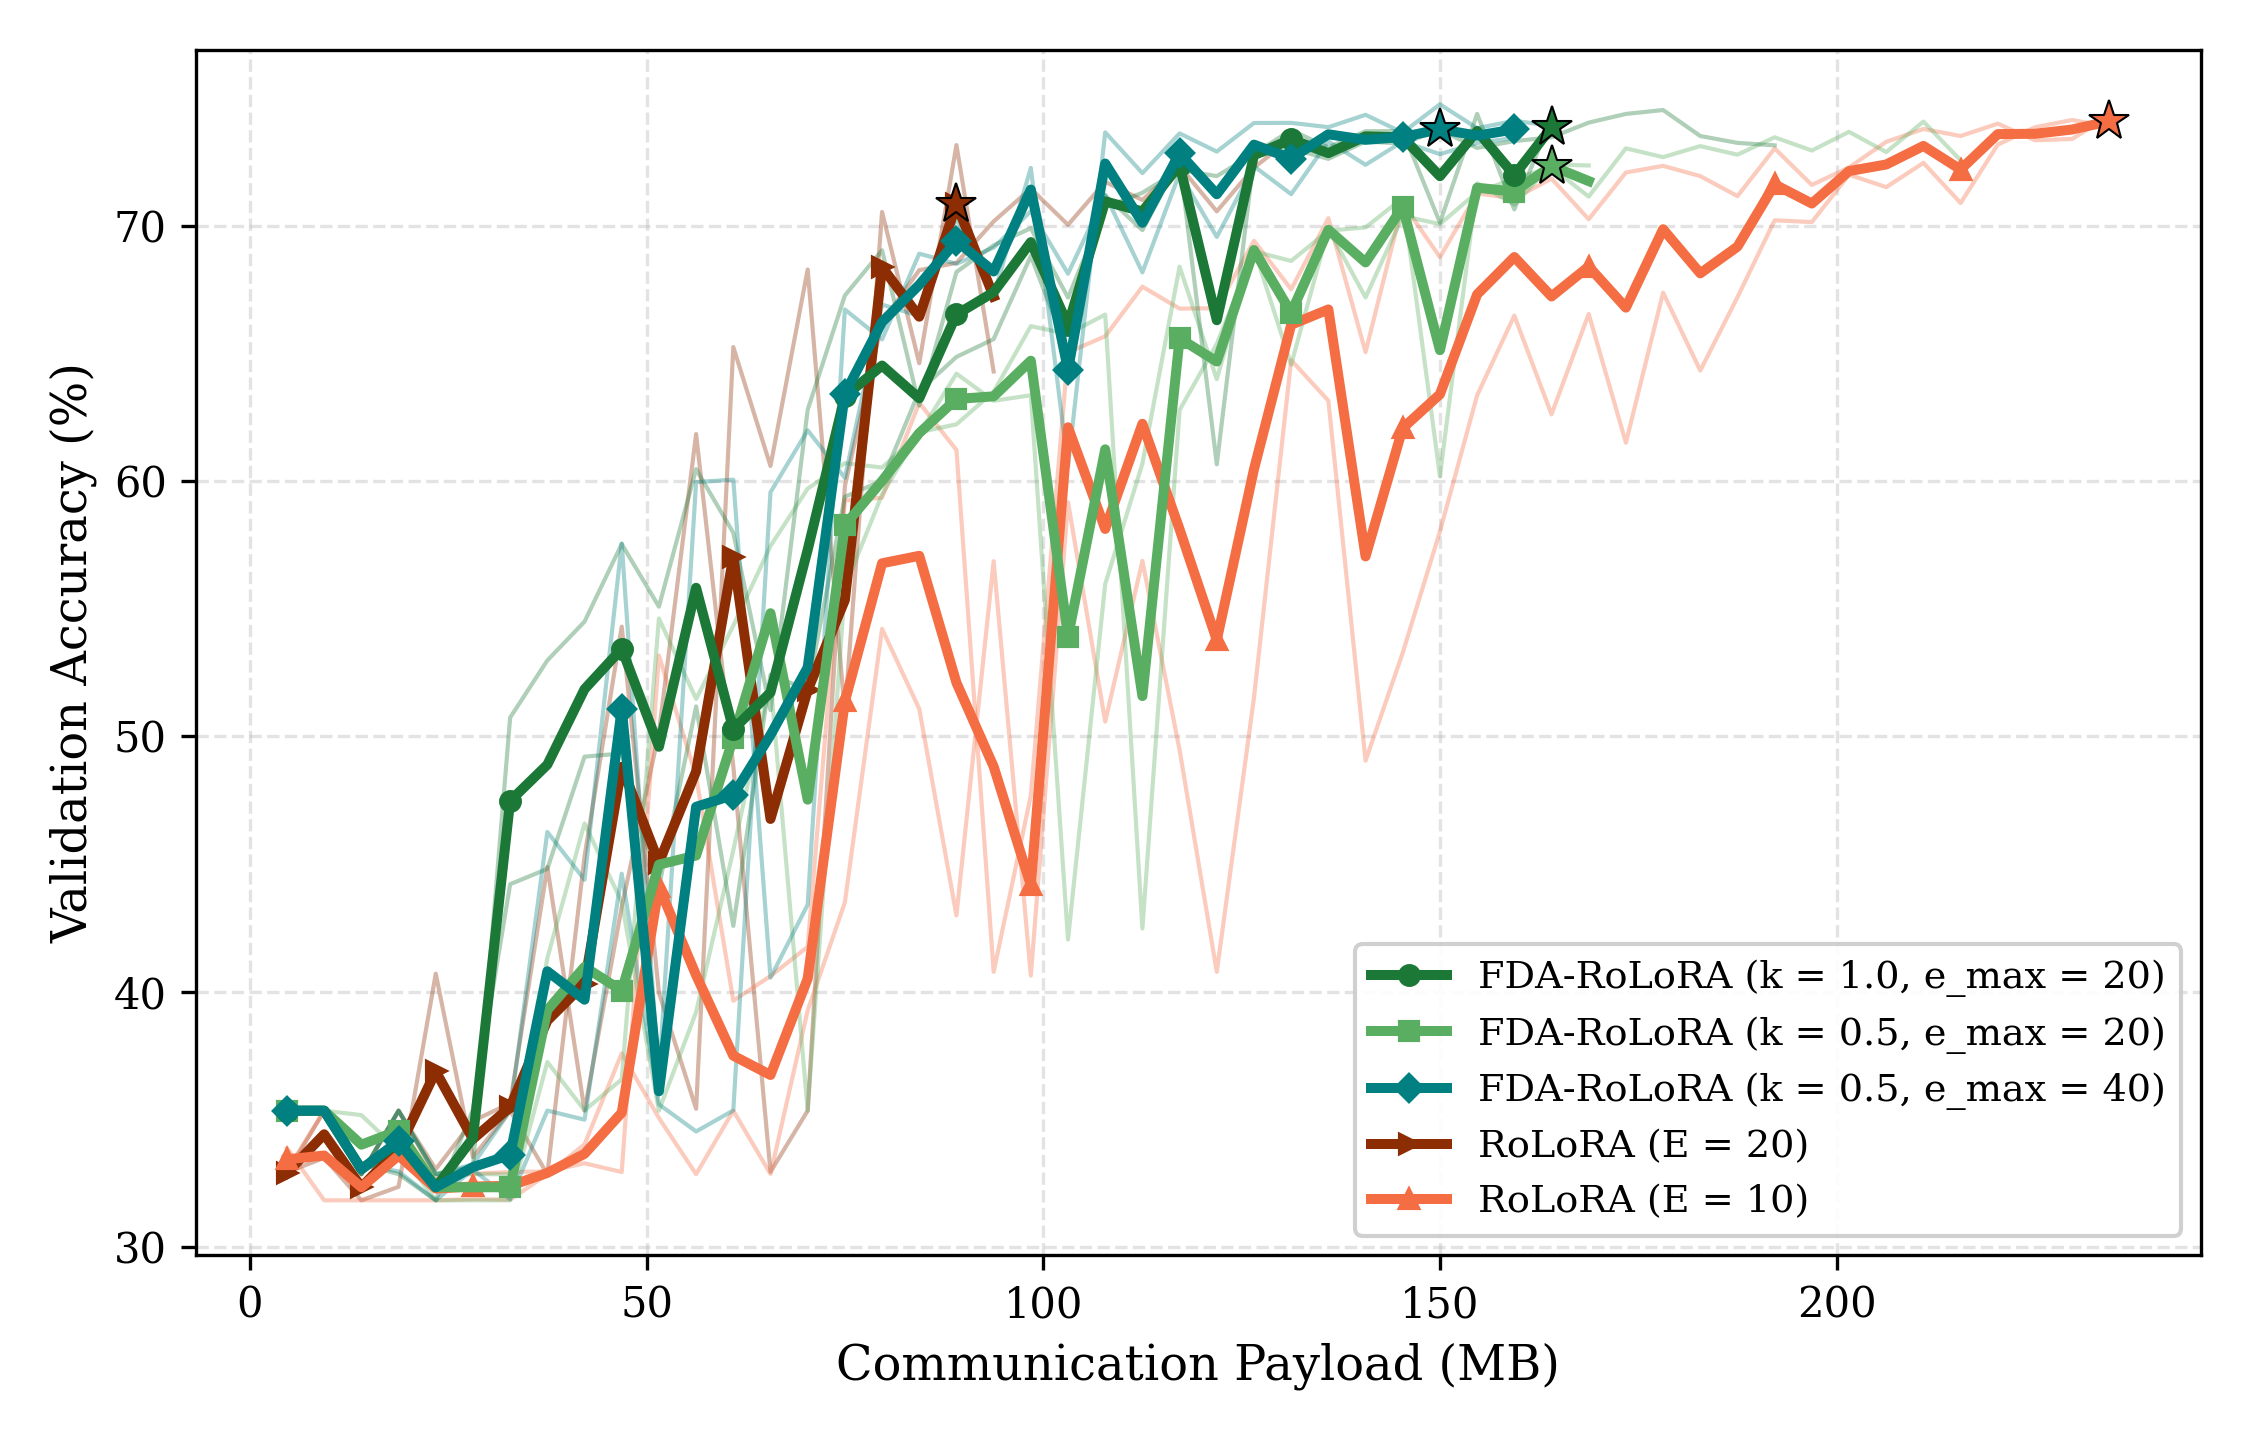
\includegraphics[width=\textwidth,height=4.9cm,keepaspectratio]{figures/telemetry/17_MNLI_C20_R50_LR0.1_A0.5_4_accuracy_vs_cost.png}
            \vspace{2pt}
            \par{\footnotesize \textbf{(b)} Accuracy vs. Communication (MB)}
        \end{minipage}

        \vspace{0.6em}
        \begin{minipage}[b]{0.485\textwidth}
            \centering
            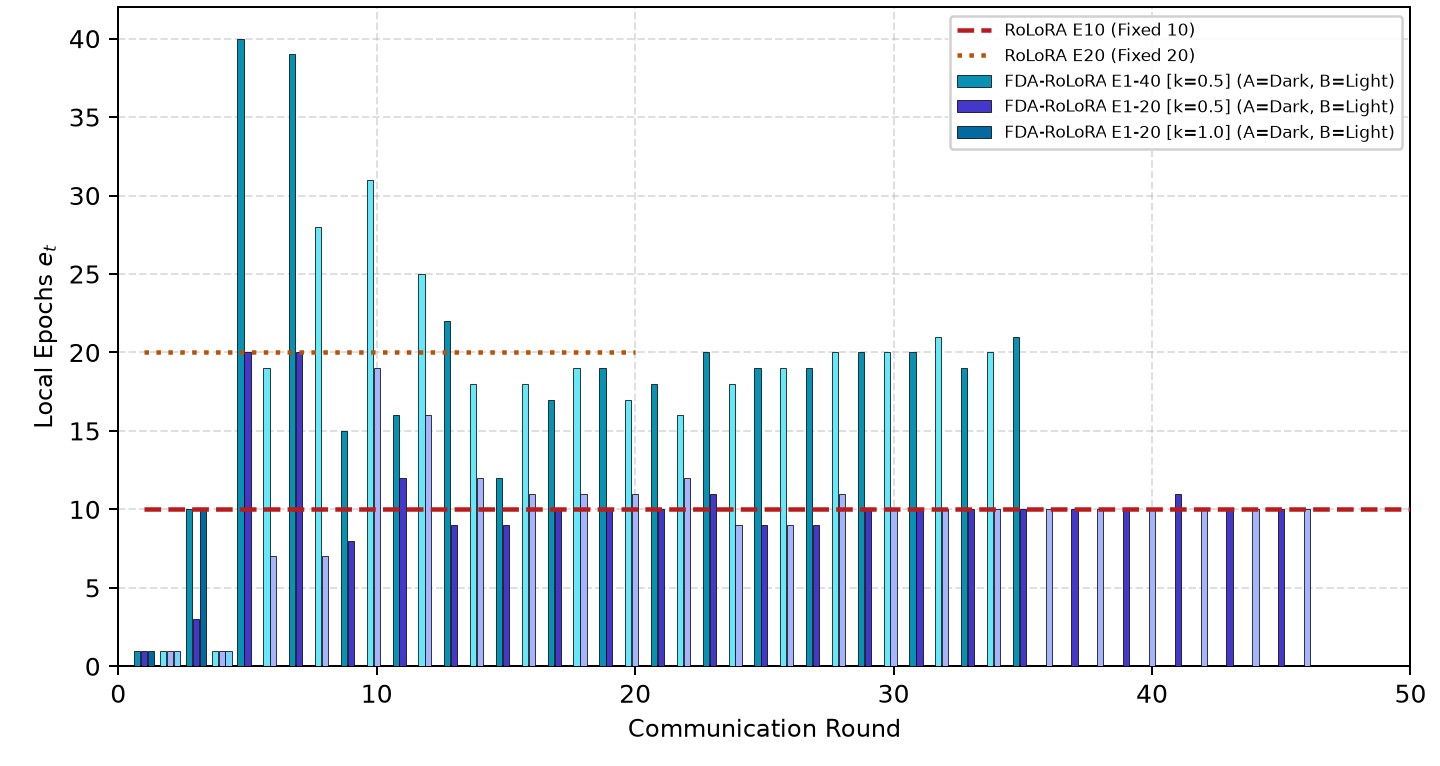
\includegraphics[width=\textwidth,height=4.9cm,keepaspectratio]{figures/telemetry/17_MNLI_C20_R50_LR0.1_A0.5_2_allocated_epochs.png}
            \vspace{2pt}
            \par{\footnotesize \textbf{(c)} Dynamic Local Epochs ($\bar{e}$)}
        \end{minipage}\hfill
        \begin{minipage}[b]{0.485\textwidth}
            \centering
            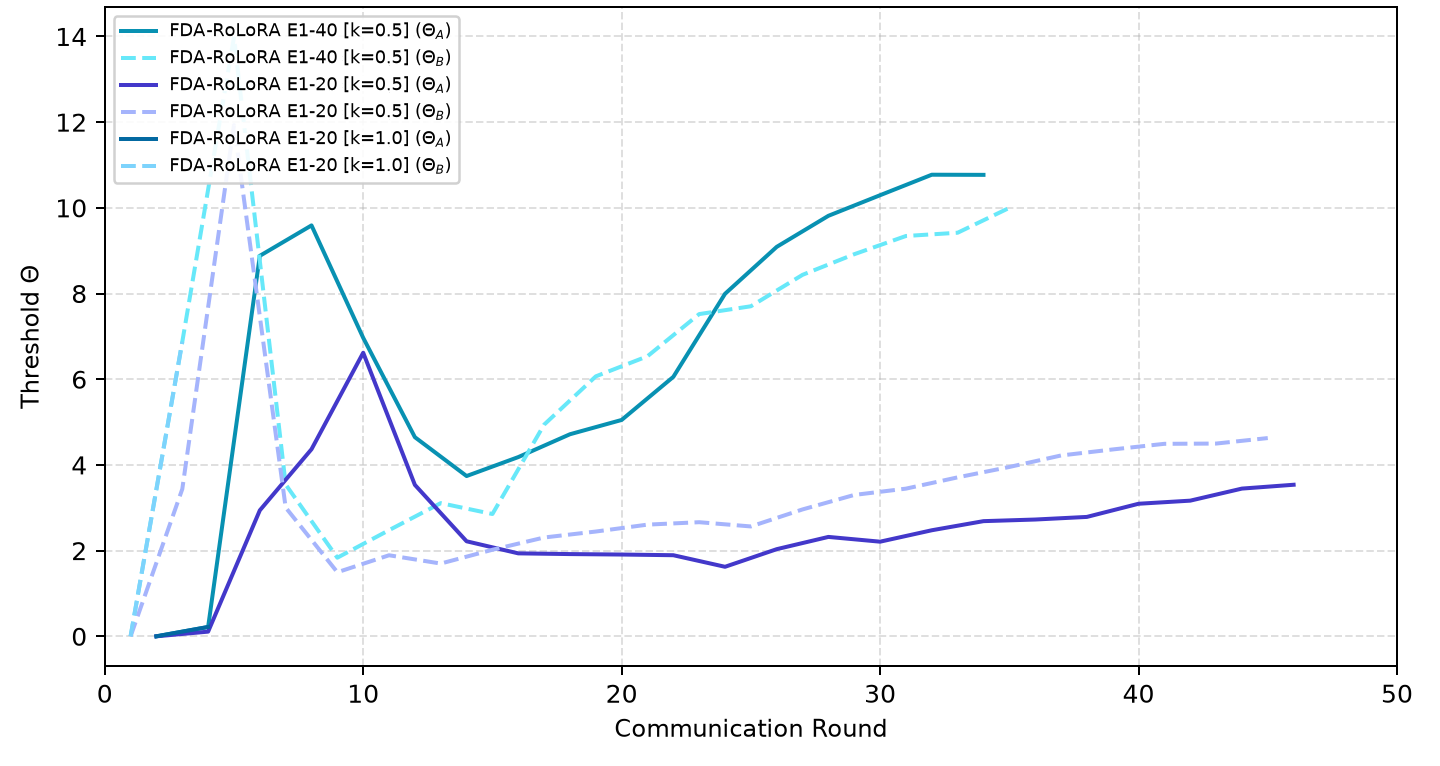
\includegraphics[width=\textwidth,height=4.9cm,keepaspectratio]{figures/telemetry/17_MNLI_C20_R50_LR0.1_A0.5_5_fda_threshold.png}
            \vspace{2pt}
            \par{\footnotesize \textbf{(d)} Factor Thresholds ($\theta_A, \theta_B$)}
        \end{minipage}

        \vspace{0.6em}
        \begin{minipage}[b]{0.485\textwidth}
            \centering
            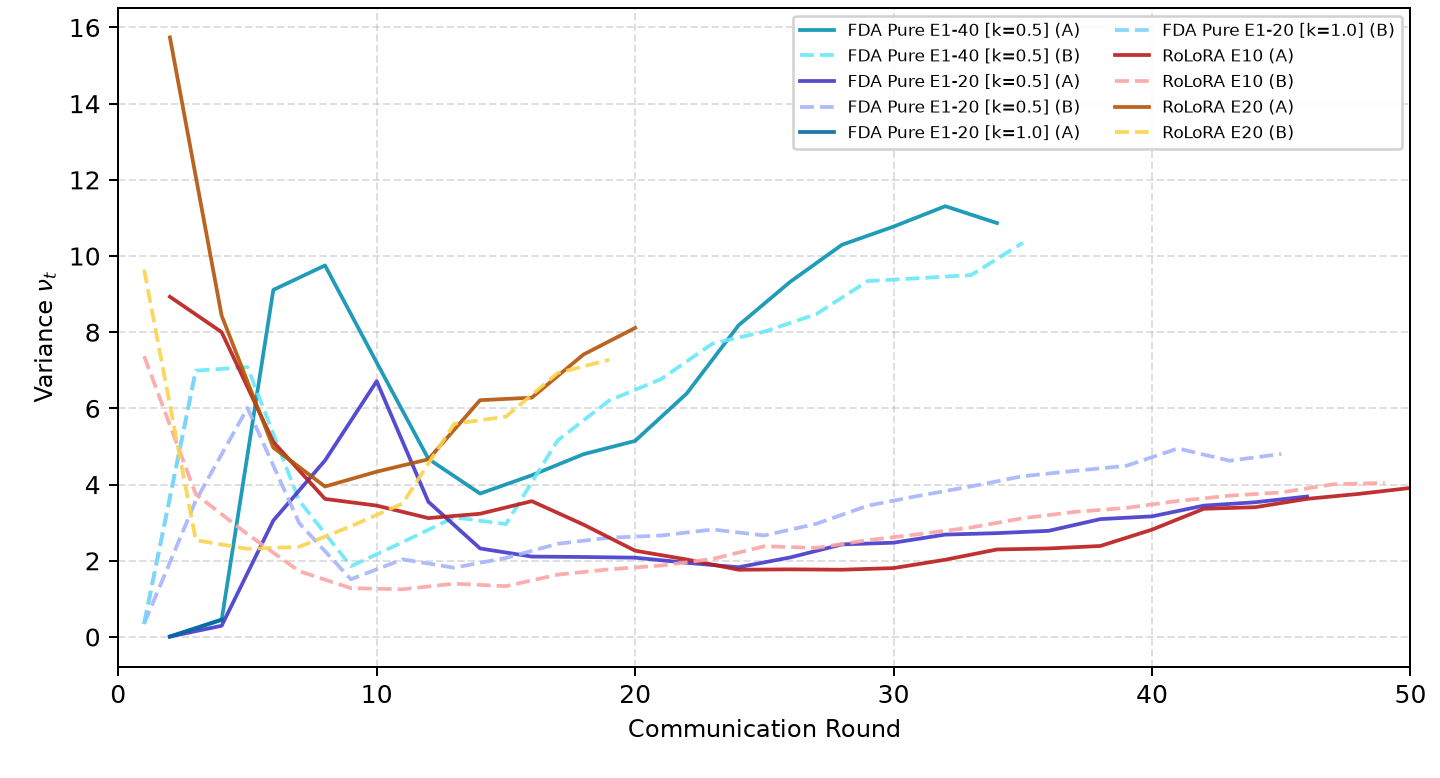
\includegraphics[width=\textwidth,height=4.9cm,keepaspectratio]{figures/telemetry/17_MNLI_C20_R50_LR0.1_A0.5_3_client_variance.png}
            \vspace{2pt}
            \par{\footnotesize \textbf{(e)} Subspace Coordinate Variance}
        \end{minipage}\hfill
        \begin{minipage}[b]{0.485\textwidth}
            \centering
            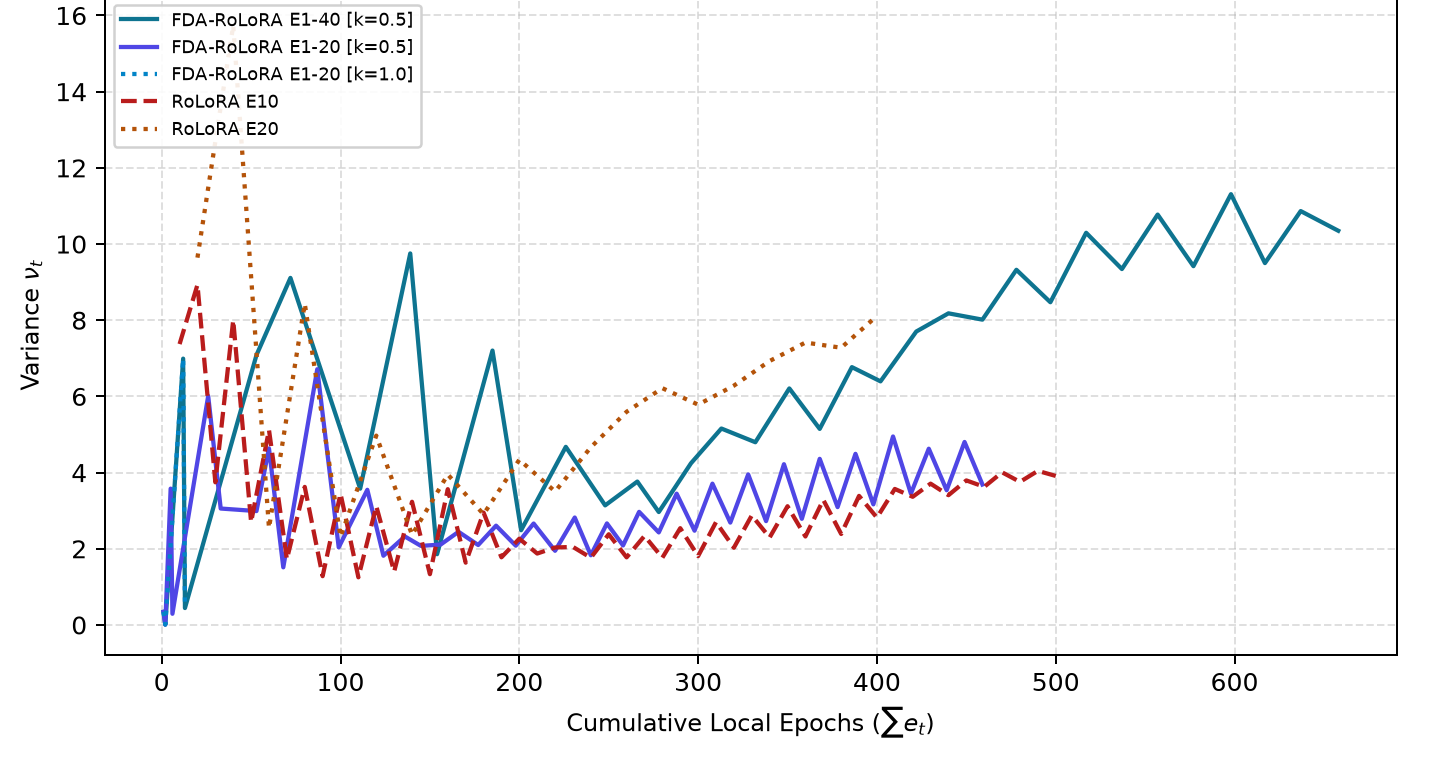
\includegraphics[width=\textwidth,height=4.9cm,keepaspectratio]{figures/telemetry/17_MNLI_C20_R50_LR0.1_A0.5_6_variance_vs_epoch.png}
            \vspace{2pt}
            \par{\footnotesize \textbf{(f)} Variance vs.\ Cumulative Local Epochs}
        \end{minipage}

        \vspace{0.6em}
        \caption{Multi-panel optimization telemetry on MNLI under Dirichlet label skew ($\alpha=0.5, C=20, R_{\max}=50, \eta_c=0.1$) comparing FDA-RoLoRA against static baselines.}
        \label{fig:telemetry_mnli_non_iid}
    \end{minipage}%
    }
\end{figure}

\paragraph{QNLI: Scalability \& Suite-Leading Peak Accuracy.}
Binary question-answering under skew demonstrates the scalability of closed-loop synchronization across the six telemetry dimensions (Figure~\ref{fig:telemetry_qnli_non_iid}). On $C=20$ ($R_{\max}=50$), FDA-RoLoRA ($k=1.0$) attains the highest peak validation accuracy across the entire non-IID benchmark suite ($\mathbf{84.22\%}$, Panel a), dominating the communication-cost curve (Panel b) over static baselines. With an expanded ceiling $e_{\max}=40$, the controller successfully expands local computation to $\bar{e} = 29.83$ epochs (Panel c) while tracking smooth, decoupled factor thresholds $\theta_A$ and $\theta_B$ (Panel d). Drift variance at synchronization (Panel e) stabilizes at $\bar{\nu} \approx 1.79$.

When scaling to $C=50$ clients under acute skew ($R_{\max}=30$), aggressive setpoint scaling ($k=1.0$) over-allocated local epochs in early rounds, precipitating client drift and tripping early stopping at round 13.0 ($152.3\,\text{MB}$, $49.51\%$ accuracy). With midpoint scaling ($k=0.5$), FDA-RoLoRA reaches a peak of $75.69 \pm 1.66\%$ (RoLoRA $E=10$: $74.61 \pm 10.15\%$), but both FDA-RoLoRA variants end near chance level (final $49.51\%$ for $k=1.0$ and $50.13\%$ for $k=0.5$), so no communication saving is claimed for this configuration. The $k=1.0$ runs used a round budget of $R_{\max}=22$.
\begin{figure}[p]
    \centering
    \makebox[\textwidth][c]{%
    \begin{minipage}{1.06\textwidth}
        \begin{minipage}[b]{0.485\textwidth}
            \centering
            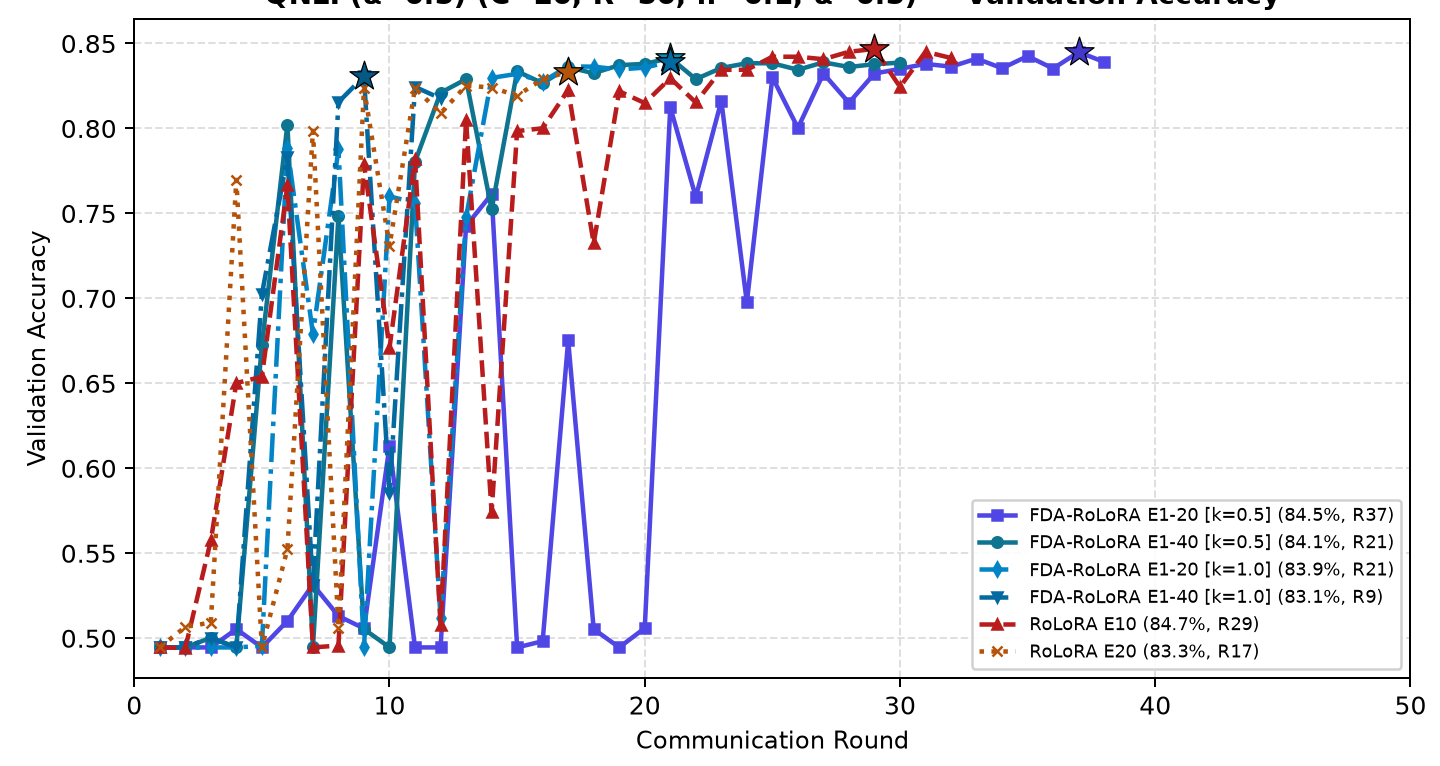
\includegraphics[width=\textwidth,height=4.9cm,keepaspectratio]{figures/telemetry/18_QNLI_C20_R50_LR0.1_A0.5_1_accuracy.png}
            \vspace{2pt}
            \par{\footnotesize \textbf{(a)} Validation Accuracy}
        \end{minipage}\hfill
        \begin{minipage}[b]{0.485\textwidth}
            \centering
            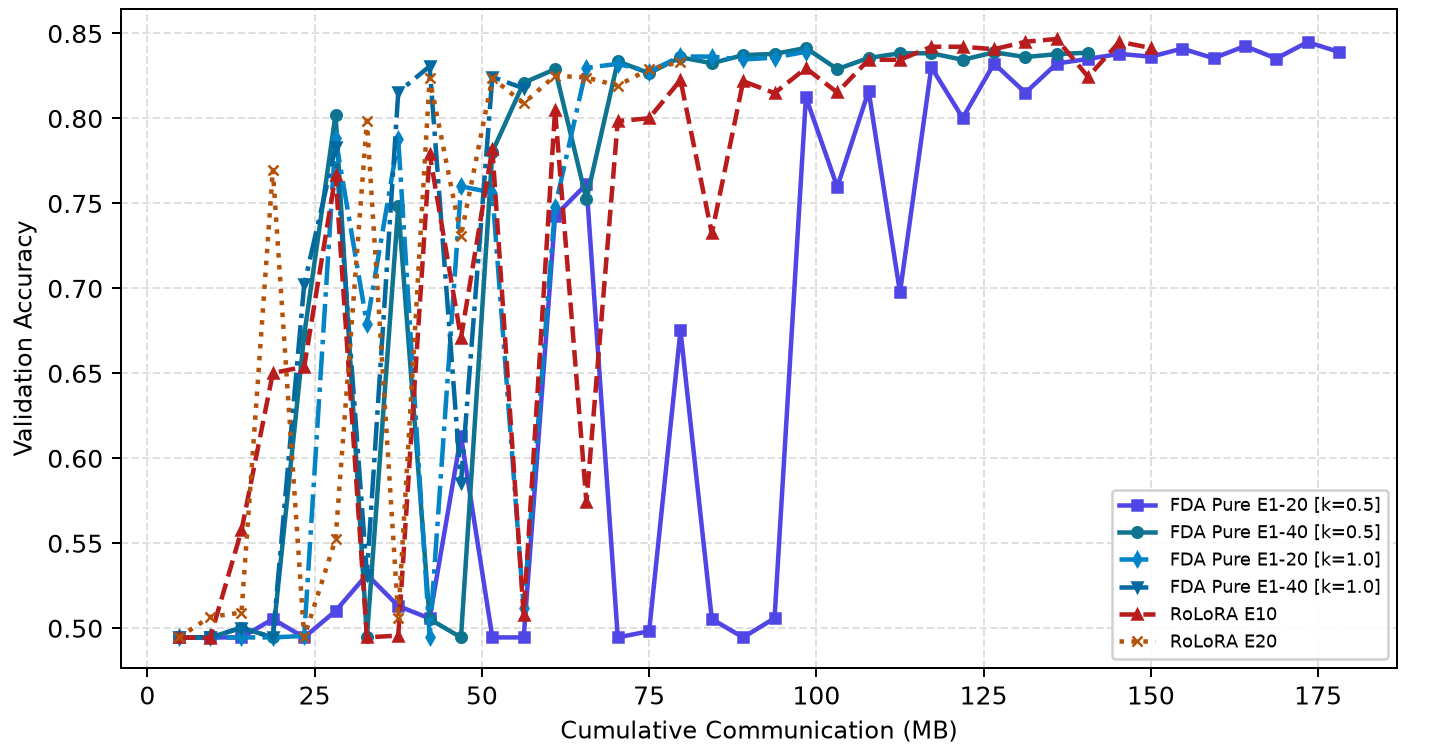
\includegraphics[width=\textwidth,height=4.9cm,keepaspectratio]{figures/telemetry/18_QNLI_C20_R50_LR0.1_A0.5_4_accuracy_vs_cost.png}
            \vspace{2pt}
            \par{\footnotesize \textbf{(b)} Accuracy vs. Communication (MB)}
        \end{minipage}

        \vspace{0.6em}
        \begin{minipage}[b]{0.485\textwidth}
            \centering
            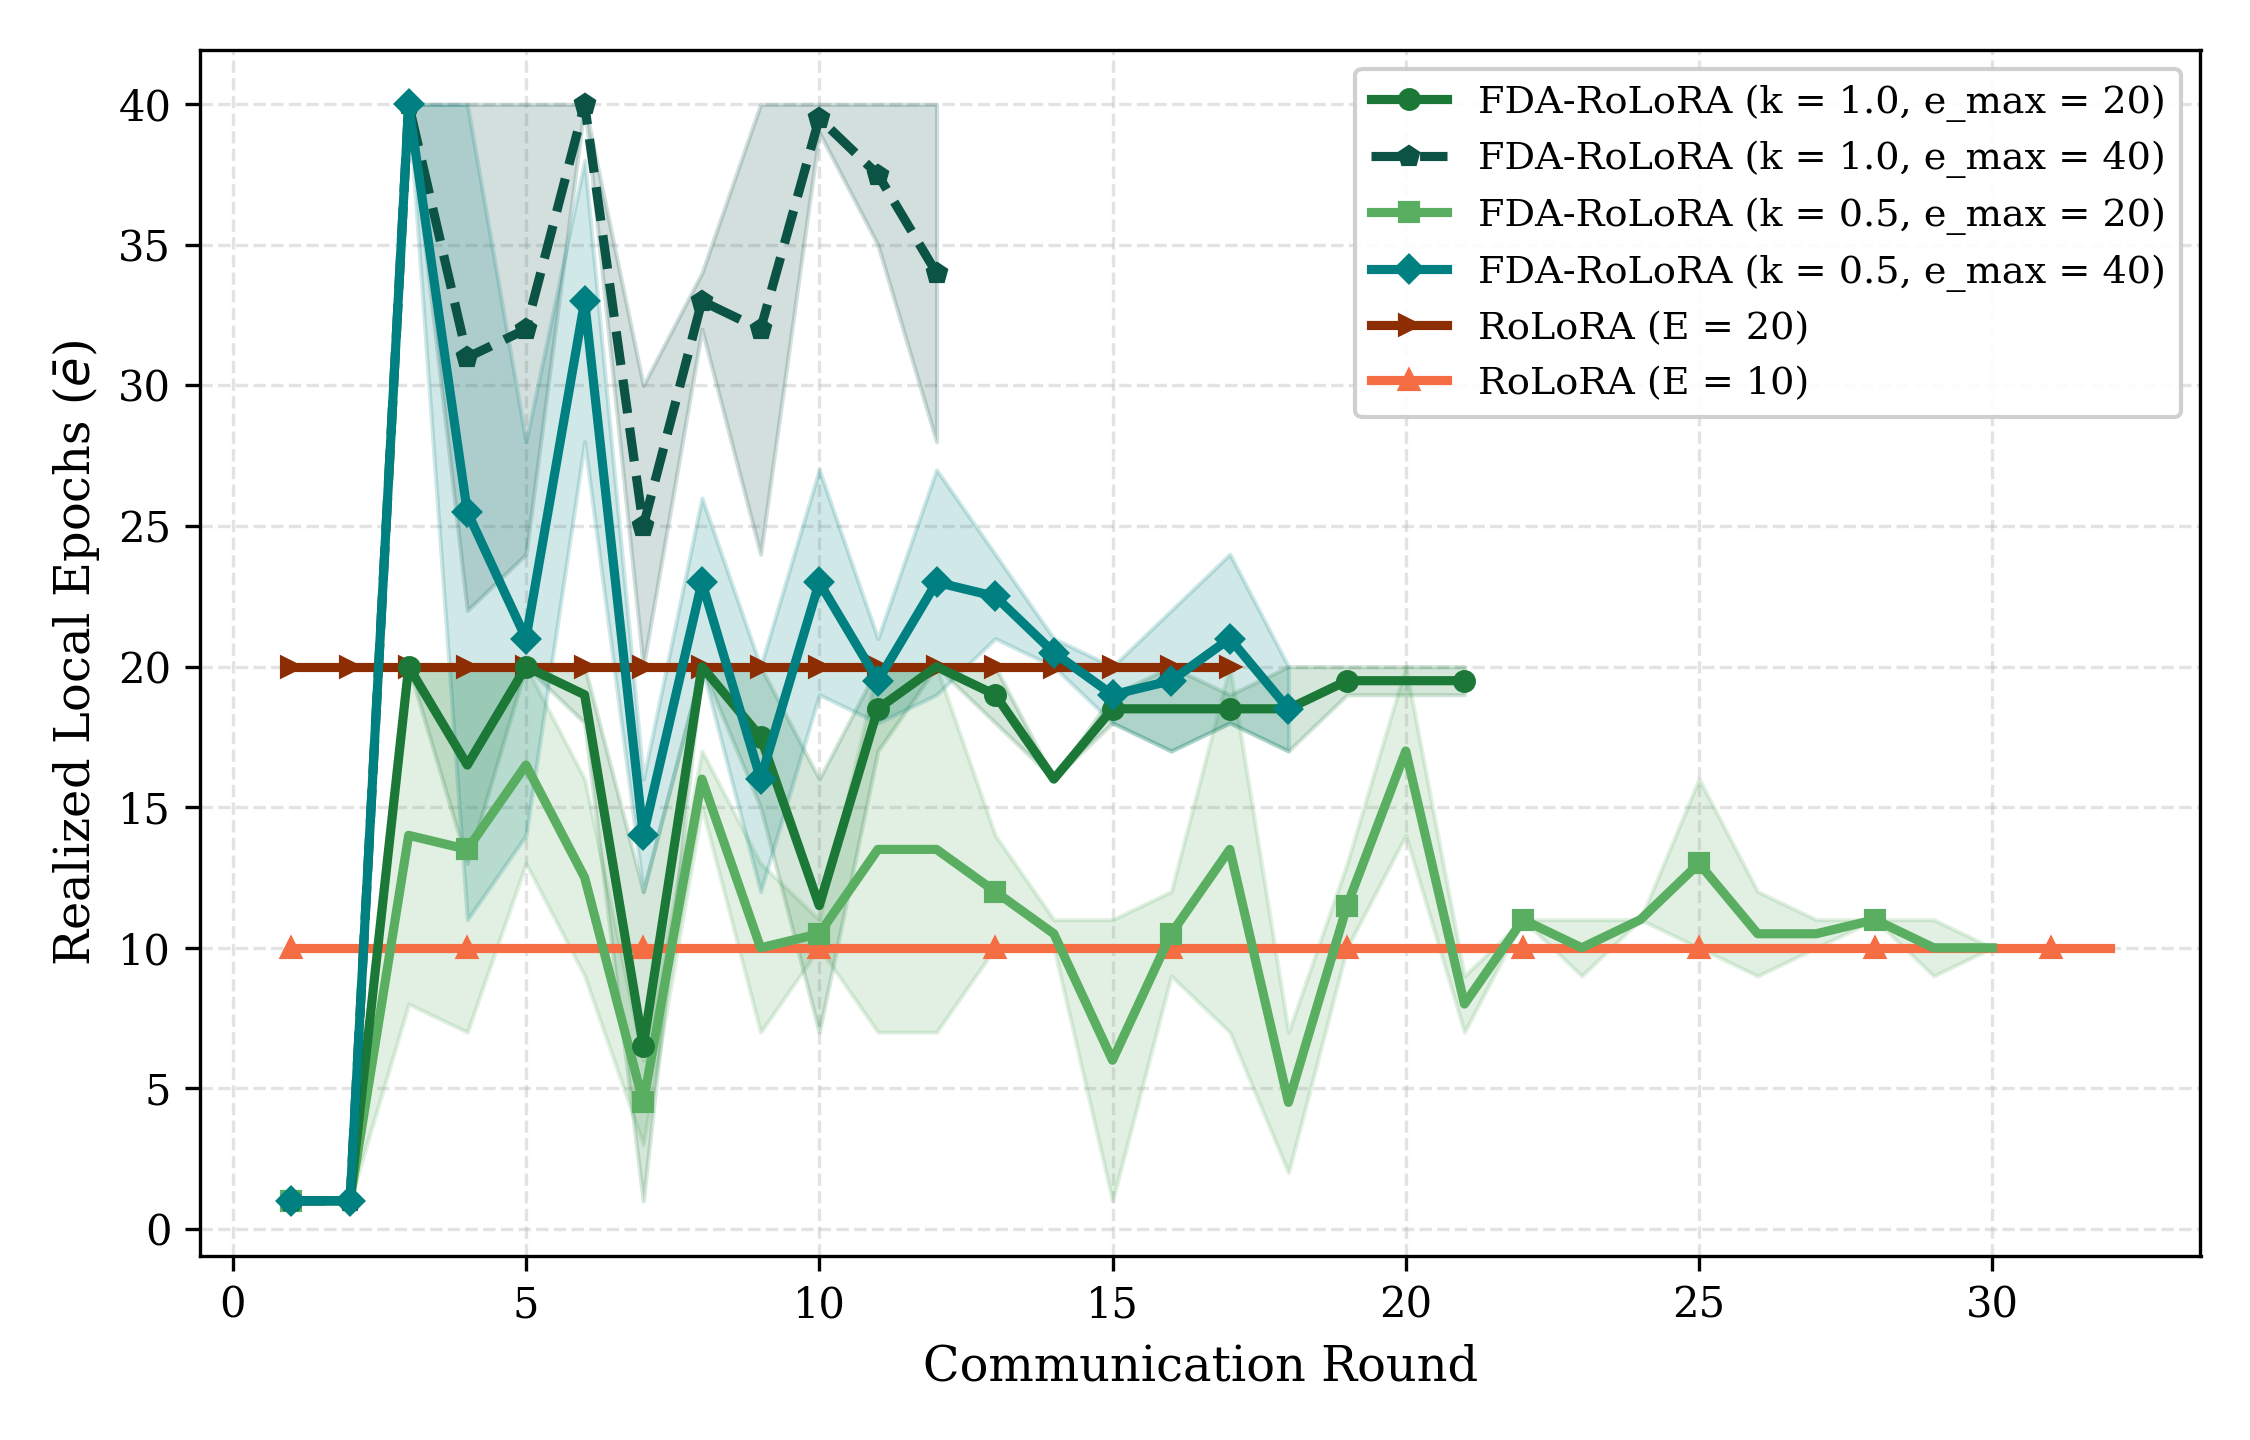
\includegraphics[width=\textwidth,height=4.9cm,keepaspectratio]{figures/telemetry/18_QNLI_C20_R50_LR0.1_A0.5_2_allocated_epochs.png}
            \vspace{2pt}
            \par{\footnotesize \textbf{(c)} Dynamic Local Epochs ($\bar{e}$)}
        \end{minipage}\hfill
        \begin{minipage}[b]{0.485\textwidth}
            \centering
            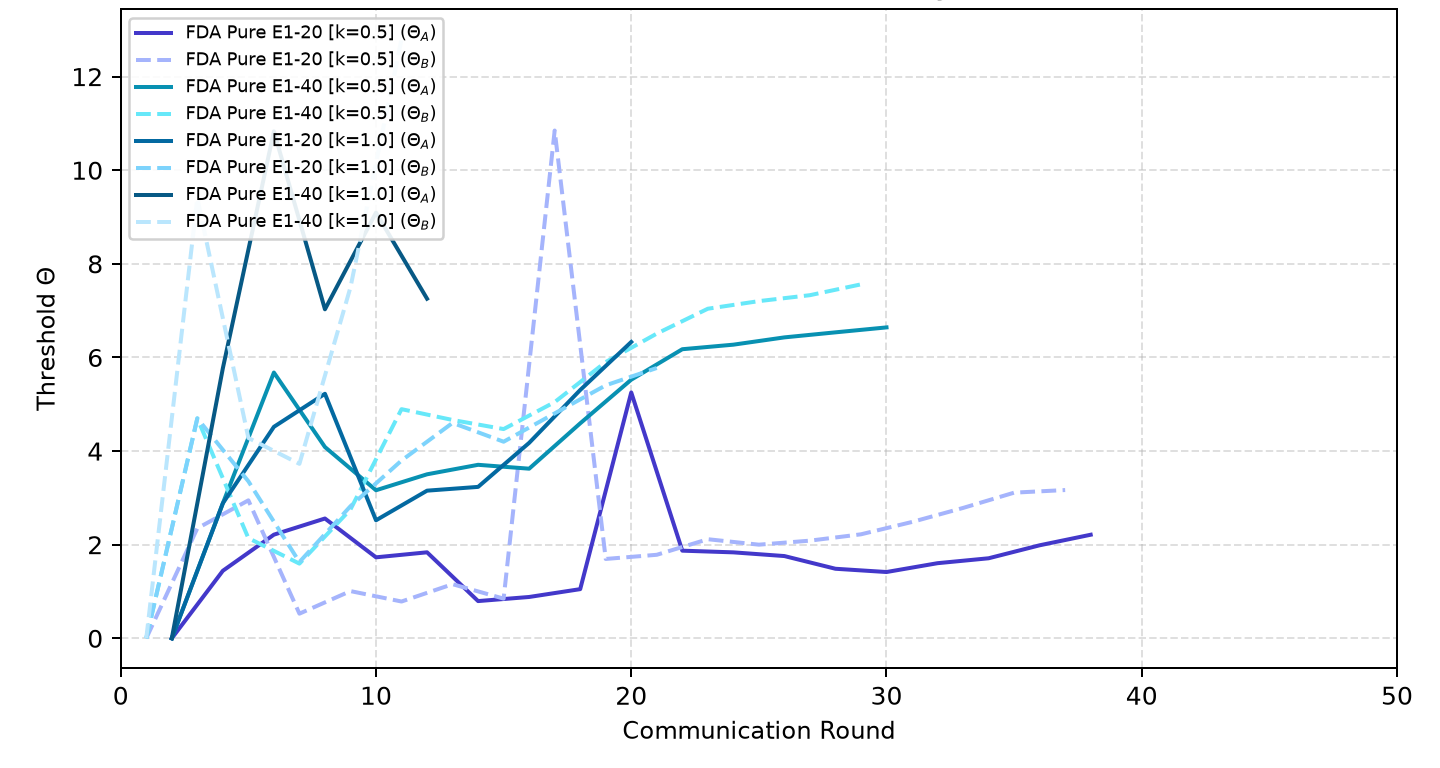
\includegraphics[width=\textwidth,height=4.9cm,keepaspectratio]{figures/telemetry/18_QNLI_C20_R50_LR0.1_A0.5_5_fda_threshold.png}
            \vspace{2pt}
            \par{\footnotesize \textbf{(d)} Factor Thresholds ($\theta_A, \theta_B$)}
        \end{minipage}

        \vspace{0.6em}
        \begin{minipage}[b]{0.485\textwidth}
            \centering
            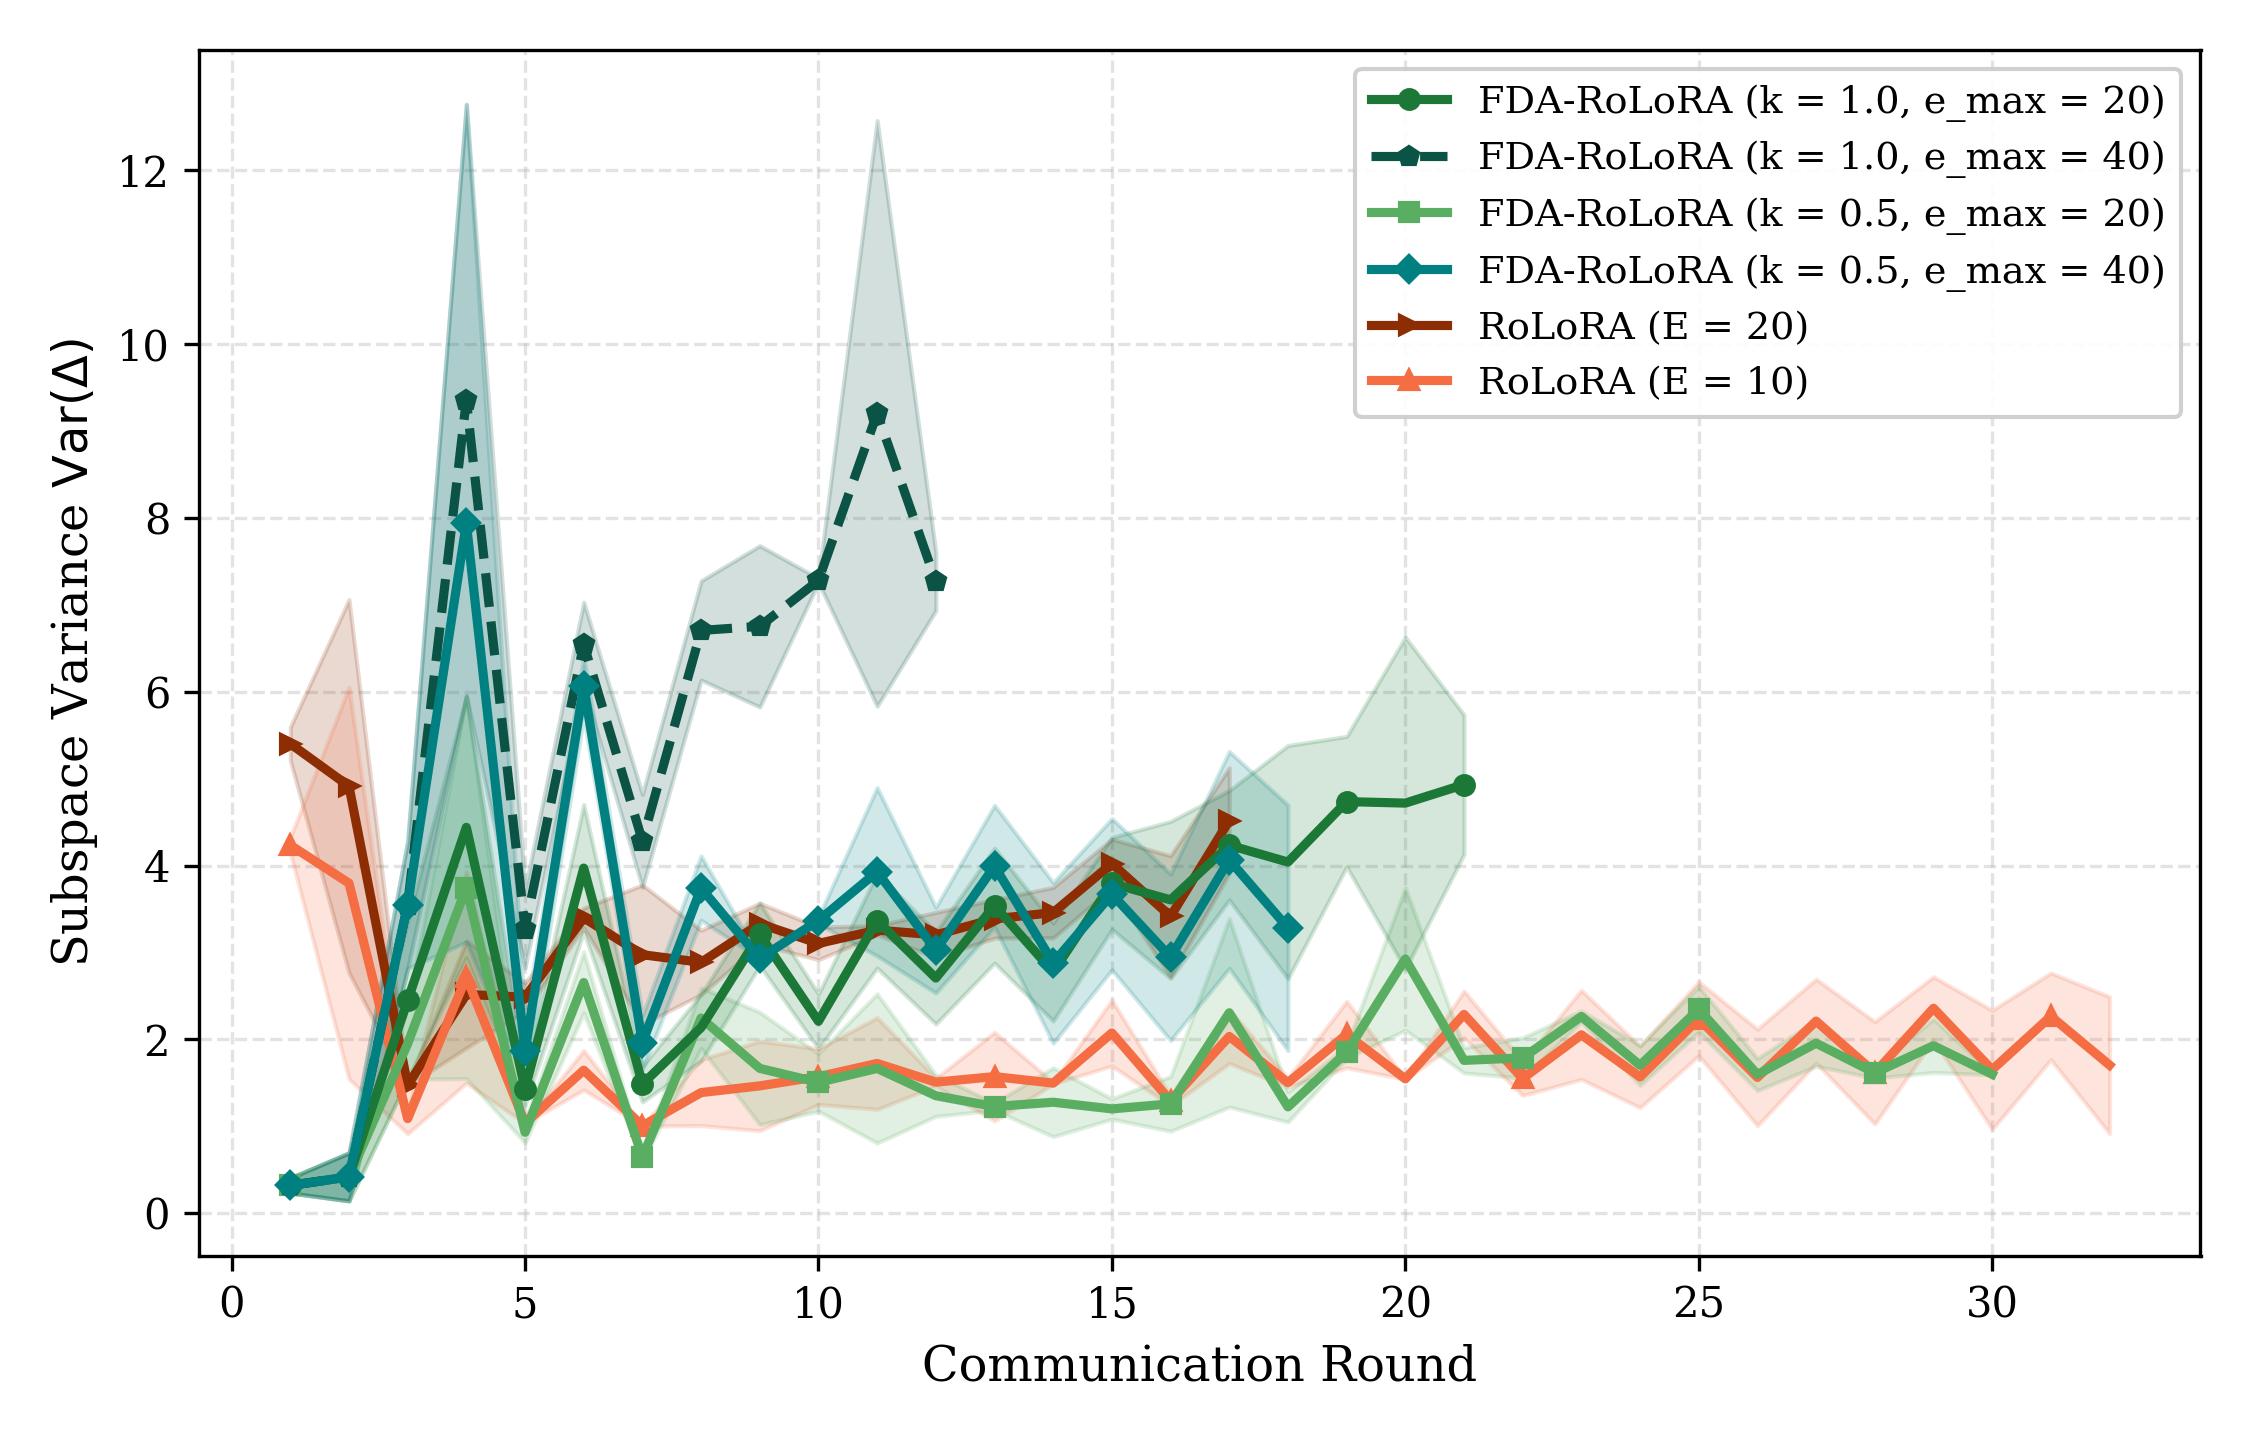
\includegraphics[width=\textwidth,height=4.9cm,keepaspectratio]{figures/telemetry/18_QNLI_C20_R50_LR0.1_A0.5_3_client_variance.png}
            \vspace{2pt}
            \par{\footnotesize \textbf{(e)} Subspace Coordinate Variance}
        \end{minipage}\hfill
        \begin{minipage}[b]{0.485\textwidth}
            \centering
            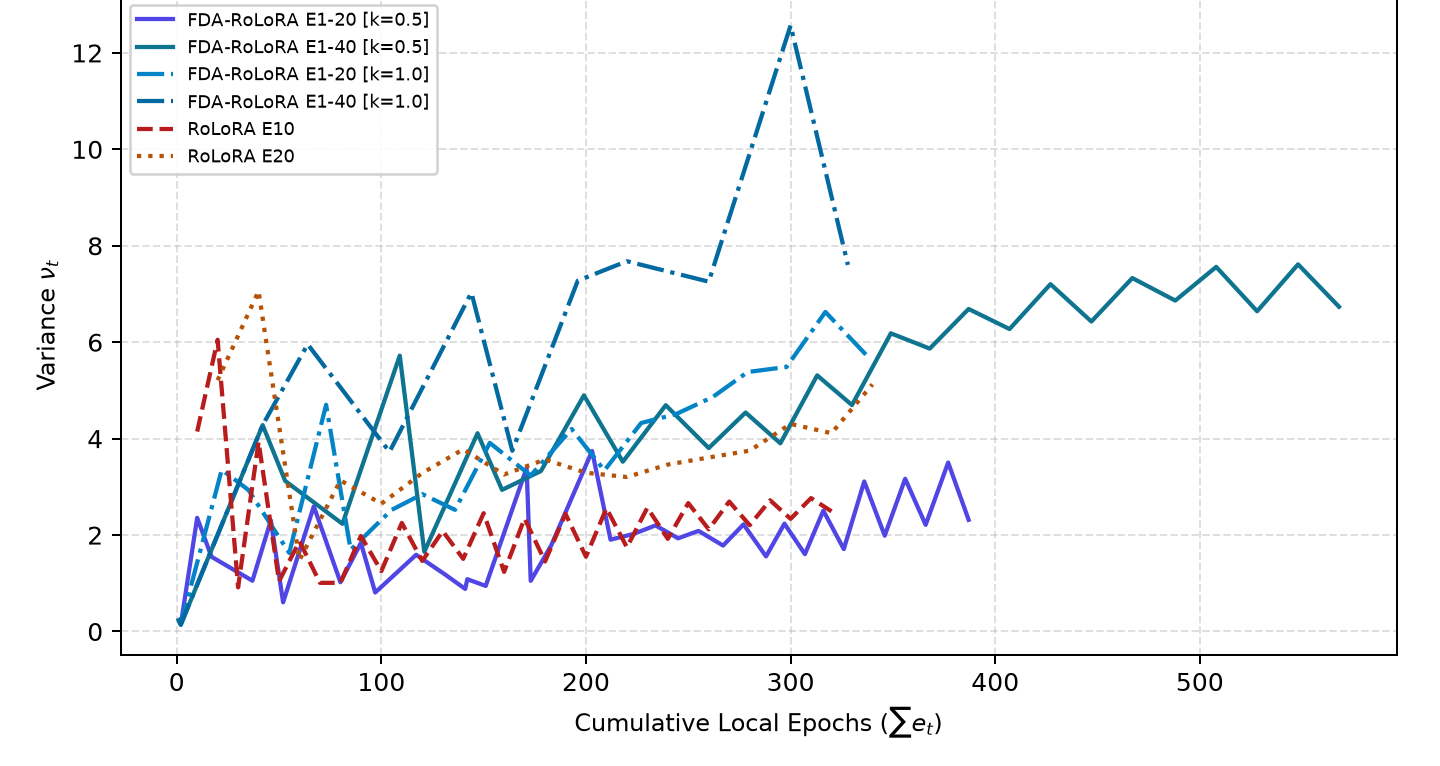
\includegraphics[width=\textwidth,height=4.9cm,keepaspectratio]{figures/telemetry/18_QNLI_C20_R50_LR0.1_A0.5_6_variance_vs_epoch.png}
            \vspace{2pt}
            \par{\footnotesize \textbf{(f)} Variance vs.\ Cumulative Local Epochs}
        \end{minipage}

        \vspace{0.6em}
        \caption{Multi-panel optimization telemetry on QNLI under Dirichlet label skew ($\alpha=0.5, C=20, R_{\max}=50, \eta_c=0.1$) comparing FDA-RoLoRA against static baselines.}
        \label{fig:telemetry_qnli_non_iid}
    \end{minipage}%
    }
\end{figure}

\paragraph{Dynamic Round Synchronization and Realized Epoch Dynamics.}
Figure~\ref{fig:non_iid_epoch_dynamics} visualizes round-by-round realized local epoch allocations on MNLI and QNLI under statistical heterogeneity. When Dirichlet skew causes local client updates to diverge sharply in coordinate space, inter-client drift variance surges by approximately $4.0\times$ (e.g., from $0.448$ to $1.794$ on QNLI). While static baselines execute a constant number of local passes regardless of parameter divergence, FDA-RoLoRA's closed-loop controller constrains local passes within $[e_{\min}, e_{\max}]$ in response to coordinate variance breaches, enforcing earlier server synchronization to mitigate client drift.

\begin{figure}[htbp]
    \centering
    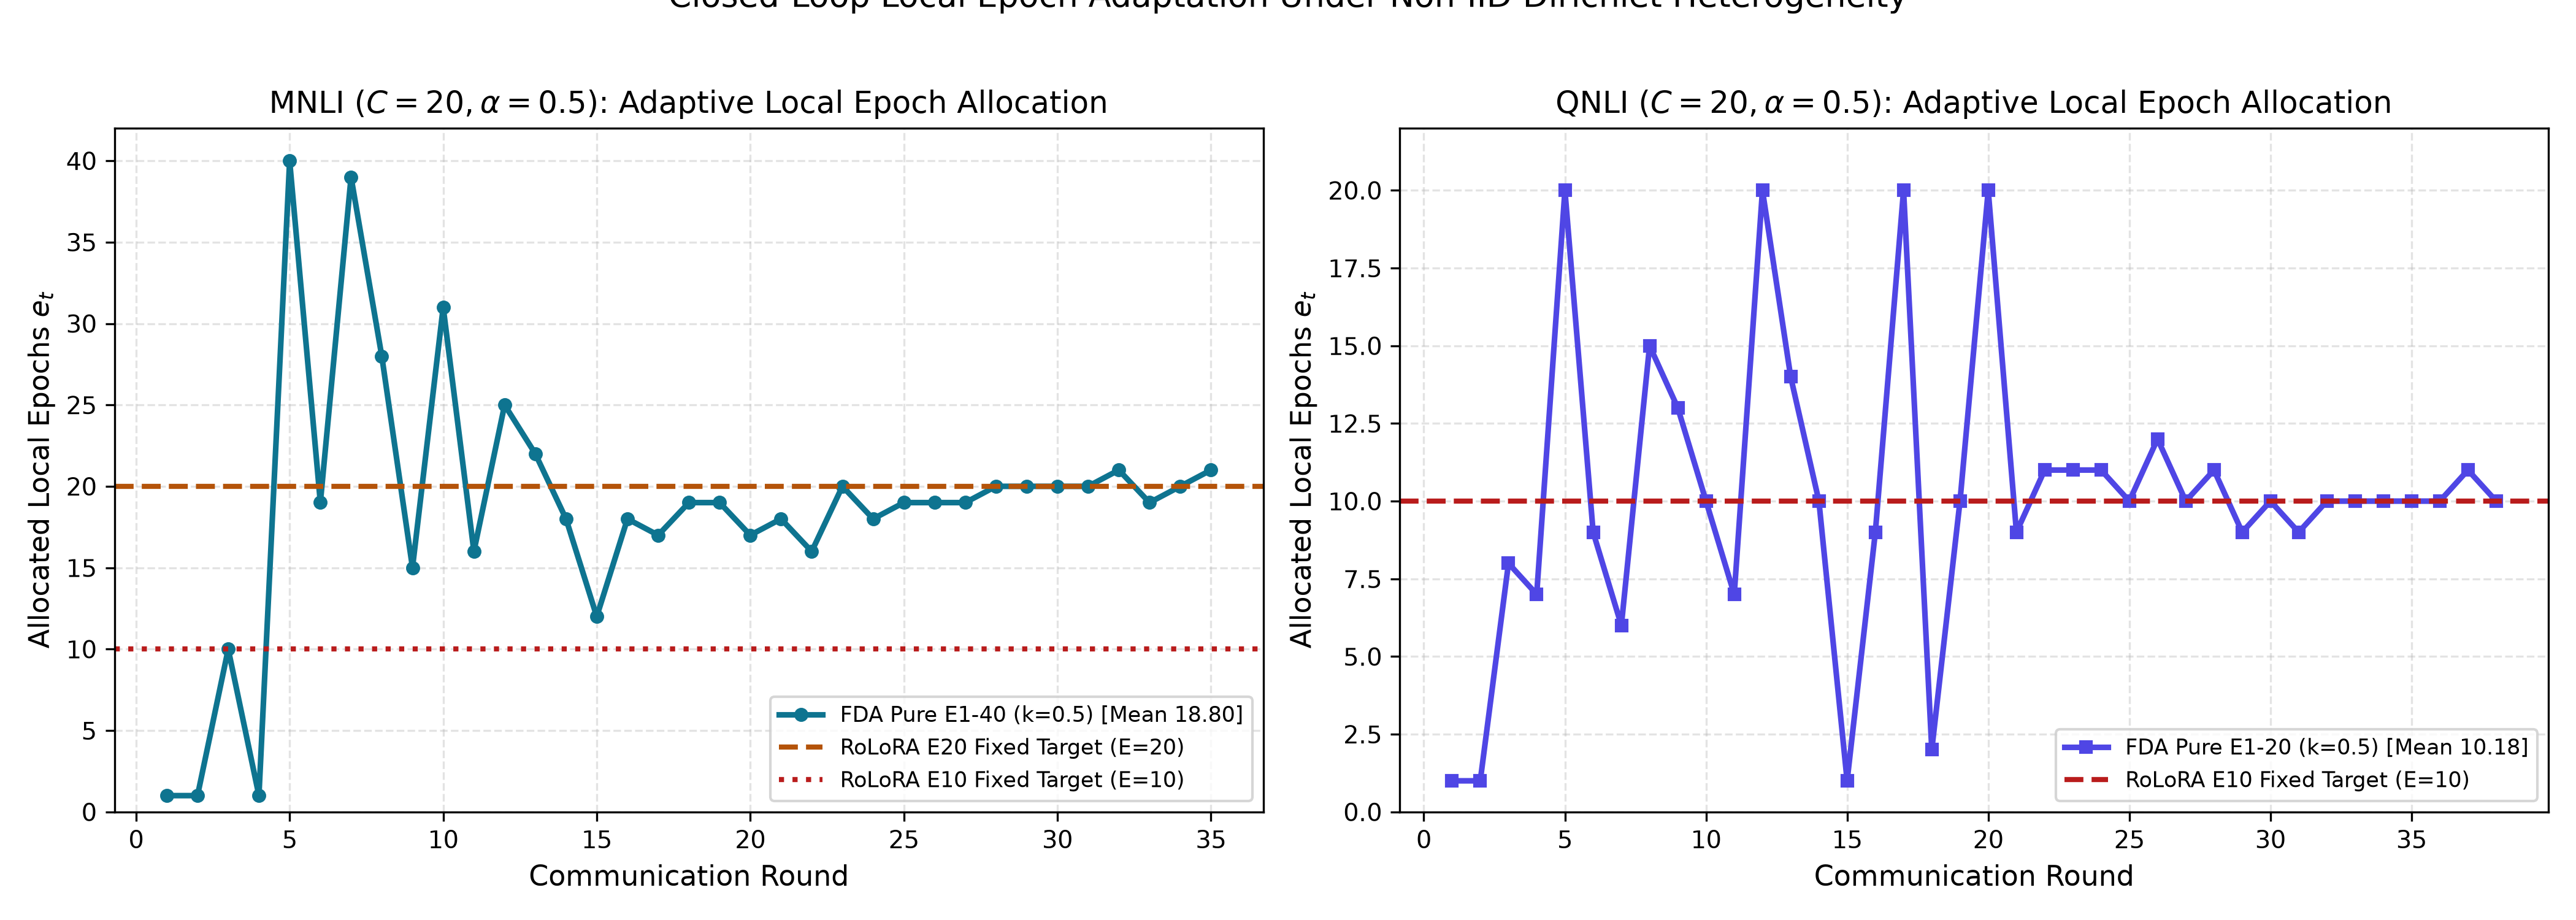
\includegraphics[width=0.95\textwidth]{figures/non_iid_epoch_dynamics.png}
    \caption{Empirical local epoch allocation dynamics under severe statistical heterogeneity (Dirichlet label skew $\alpha=0.5$), illustrating the closed-loop setpoint tracking dynamics of FDA-RoLoRA on MNLI and QNLI under Dirichlet label skew ($\alpha=0.5$).}
    \label{fig:non_iid_epoch_dynamics}
\end{figure}

\paragraph{SST-2 \& QQP: Cross-Task Drift and Anti-Collapse Protection.}
Figure~\ref{fig:non_iid_benchmark_telemetry} provides a focused diagnostic synthesis on MNLI and QNLI of federated fine-tuning under acute Dirichlet label skew ($\alpha=0.5$). The most pronounced empirical difference occurs on SST-2 with 50 clients. Under static $E=10$, RoLoRA did not leave the initial majority-class plateau within the 20-round budget in either seed (final $51.15\%$ and $55.50\%$), remaining trapped at the majority-class baseline ($\sim 50\%$) for the majority of rounds before an isolated surge to $59.00 \pm 11.11\%$ peak accuracy ($53.33 \pm 3.08\%$ final). In contrast, FDA-RoLoRA ($k=1.0$) dynamically navigated the loss landscape to escape the plateau, attaining $\mathbf{85.95 \pm 5.60\%}$ peak accuracy (final $88.42\%$ and $74.31\%$ in the two seeds), with a higher mean local-epoch count ($\bar{e}=14.57$ vs.\ 10), representing a \textbf{+26.95\% absolute improvement in peak accuracy}. On QQP ($C=50$), FDA-RoLoRA stops earlier (15.5 vs.\ 22.5 rounds), but one seed ended at chance level ($49.46\%$), and its mean final accuracy ($57.45\%$) is below RoLoRA $E=10$ ($69.28\%$). The earlier stop is therefore not a saving at equal accuracy.



\begin{figure}[htbp]
    \centering
    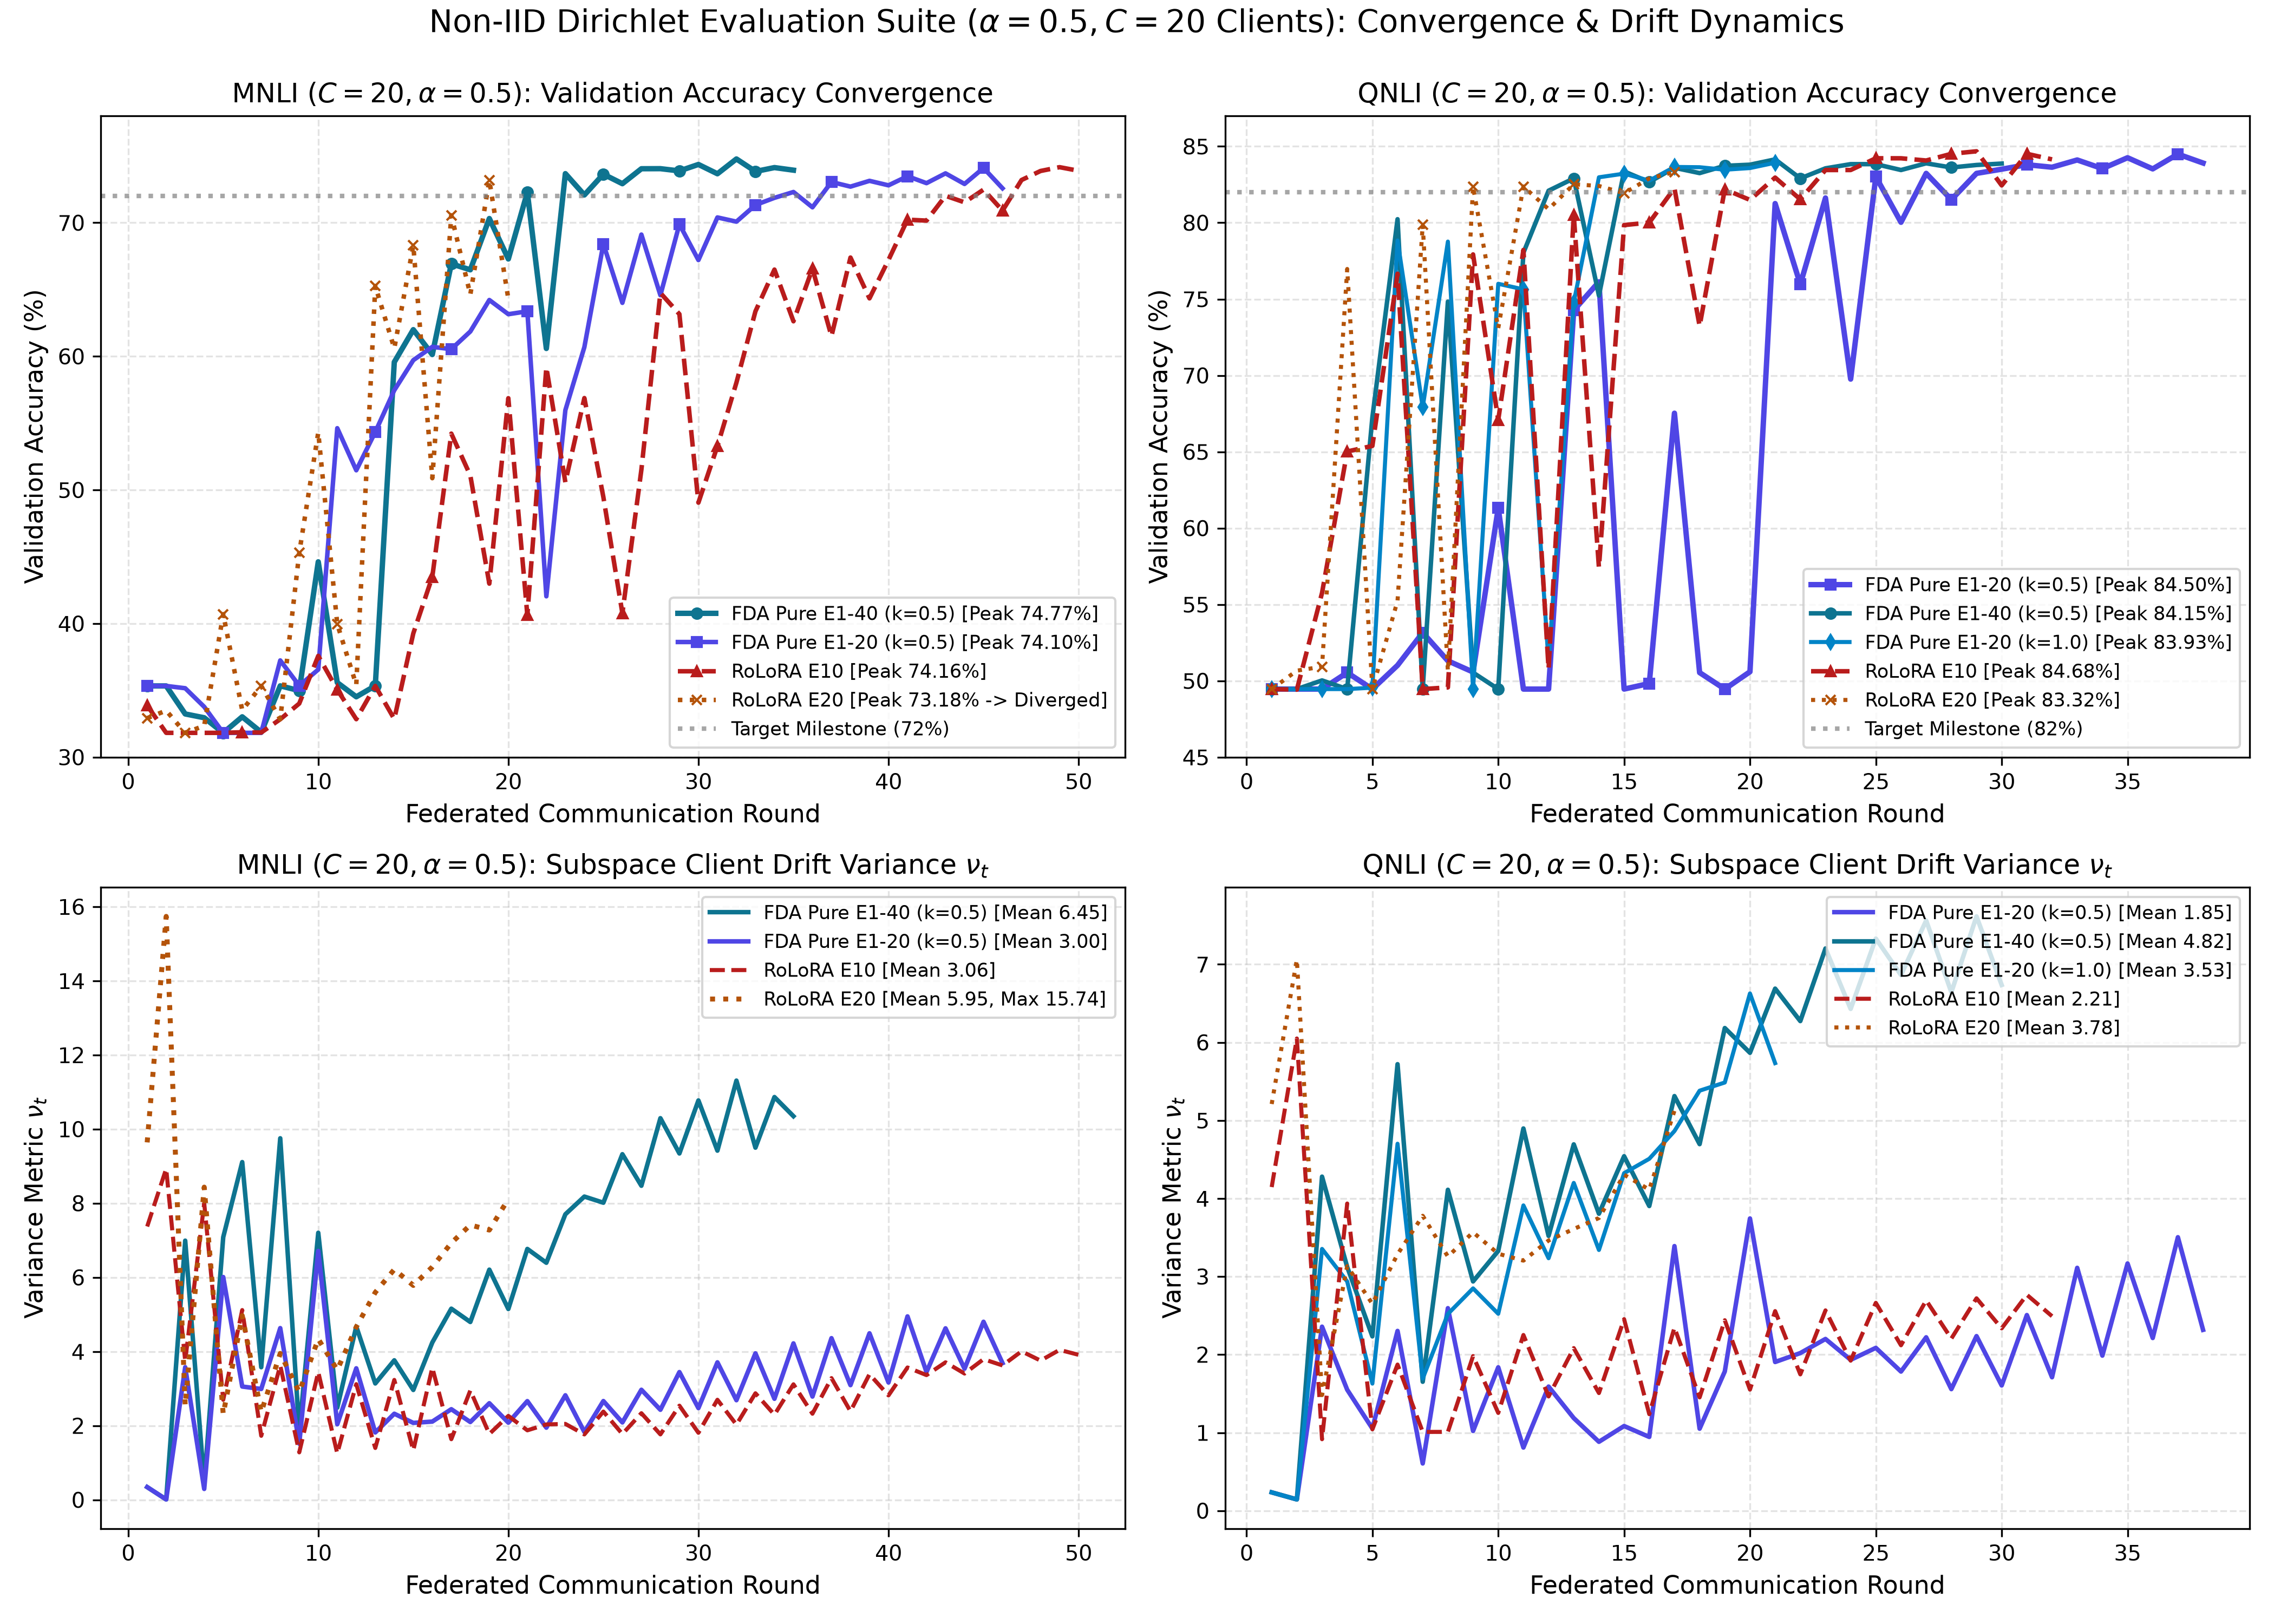
\includegraphics[width=0.95\textwidth]{figures/non_iid_benchmark_telemetry.png}
    \caption{Convergence and client drift variance trajectories on MNLI and QNLI under severe Dirichlet statistical heterogeneity ($\alpha = 0.5$). Top panels present validation accuracy trajectories; bottom panels present client coordinate drift variance ($\sigma_t^2$).}
    \label{fig:non_iid_benchmark_telemetry}
\end{figure}

\clearpage

\chapter{Conclusion and Future Work}
\label{chap:conclusion}

This thesis investigated the integration of Federated Dynamic Averaging (FDA) with Parameter-Efficient Low-Rank Adaptation (LoRA) in federated learning. By formulating and analyzing FDA-RoLoRA---which couples alternating low-rank parameter optimization with an internal dual-track threshold mechanism---this work examined how variance-driven dynamic synchronization can be coupled with alternating low-rank parameter optimization to jointly address spatial parameter overhead and rigid temporal synchronization schedules under statistical data heterogeneity.

\section{Synthesis of Results and Methodological Takeaways}
\label{sec:synthesis_results}

The theoretical formulation, algorithmic design, and empirical evaluation of FDA-RoLoRA yield several core methodological takeaways:

\begin{enumerate}
    \item \textbf{Preservation of Aggregation Linearity}: Dynamic averaging cannot be naively coupled with standard federated LoRA architectures. In simultaneous factor adaptation, bilinear aggregation error---where $\frac{1}{N}\sum A_i B_i \neq (\frac{1}{N}\sum A_i)(\frac{1}{N}\sum B_i)$---distorts local client drift trajectories, causing variance monitoring to misdiagnose true model divergence. By adopting alternating coordinate optimization, the parameter space is restricted to a single factor ($A$ or $B$) per communication round. This guarantees strict linearity in parameter updates, providing the necessary mathematical substrate for stable, decoupled subspace variance tracking without cross-matrix geometric distortion.
    
    \item \textbf{Decoupled Subspace Geometric Monitoring}: Evaluating drift variance directly on isolated low-rank coordinate tensors eliminates the memory and communication overhead of full-model gradient approximations and high-dimensional sketching. By operating an internal dual-track threshold mechanism ($\theta_A, \theta_B$), the system regulates synchronization intervals via a responsive, parameter-free midpoint scaling controller that dynamically calibrates local epoch counts according to realized drift variance on the active coordinate subspace. Establishing the direct Standard update rule as the primary operational controller preserves algorithmic parsimony while maintaining responsive adaptation to local drift.
    
    \item \textbf{Empirical Foundation Model Benchmarks}: Empirical evaluations across transformer foundation models (\texttt{roberta-base} on GLUE tasks) demonstrate that dynamic synchronization achieves substantial communication round savings while preserving model accuracy under statistical data heterogeneity.
\end{enumerate}

\section{Limitations}
\label{sec:limitations}

The methodology and conclusions presented in this work should be considered alongside several operational and experimental limitations:

\begin{enumerate}
    \item \textbf{Empirical Scope and Model Diversity}: While evaluated on \texttt{roberta-base}, extensive multi-seed verification across diverse autoregressive language models and varying non-IID Dirichlet concentration regimes remains valuable future work.
    
    \item \textbf{Simulated Distributed Environment}: Due to the lack of access to the original codebase from the RoLoRA literature, our framework relies on an independent, custom reimplementation. Furthermore, evaluations are conducted within a simulated multi-process federated environment on centralized GPU infrastructure ($2\times$ NVIDIA A10 GPUs), leaving real-world distributed network constraints---such as physical transit latency, asymmetric bandwidth, and stochastic client dropouts---unmodeled.
    
    \item \textbf{Rank Scalability and Alternation Heuristics}: While exact Euclidean variance computation on compact coordinate tensors is computationally negligible for standard low ranks ($r=8$), scaling to substantially higher ranks or wider layer coverage may eventually require approximate sketching techniques (such as the AMS sketch). Additionally, the alternating optimization protocol relies on a rigid deterministic alternation schedule, leaving adaptive or variance-driven matrix toggling criteria unaddressed.
\end{enumerate}

\section{Future Work}
\label{sec:future_work}

Building upon the findings established in this thesis, subsequent research should prioritize several promising directions:

\begin{enumerate}
    \item \textbf{Broader Foundation Model Exploration}: Extending empirical benchmarking to larger autoregressive language models (such as LLaMA and Mistral families) and generative tasks across distributed GPU clusters will further quantify scalability under massive parameter regimes.
    
    \item \textbf{Generalization Across Federated LoRA Variants}: Extending dynamic variance monitoring to alternative parameter-efficient federated paradigms. Key directions include investigating \textbf{FDA + SLoRA} \cite{babakniya2023slora} for coordinate-sparse parameter exchanges, \textbf{FDA + FFA-LoRA} \cite{sun2024improving} with permanently frozen down-projections, and examining whether geometric variance tracking can help diagnose and mitigate client drift in standard simultaneous \textbf{FDA + FedLoRA}. Furthermore, developing adaptive rank allocation algorithms, where the rank $r$ dynamically expands or contracts in response to observed subspace variance, represents a natural extension.
    
    \item \textbf{Advanced Controller Design}: While this thesis adopts the direct, parameter-free Standard update rule, subsequent studies should systematically examine whether advanced closed-loop feedback controllers (such as PID-regulated threshold scaling and variance-acceleration damping) can provide enhanced stability under severe distribution shifts or deeper foundation models. Concurrently, developing formal convergence proofs for alternating dynamic averaging under non-convex loss topologies constitutes an important theoretical milestone.
    
    \item \textbf{Optimization and System Hardening}: From an optimization perspective, exploring asymmetric learning rate schedules tailored independently for down-projection ($A$) and up-projection ($B$) matrices offers potential convergence gains. In addition, architectural integration with low-bit quantization frameworks (such as QLoRA \cite{dettmers2023qlora}) and deployment over physical edge testbeds will further establish operational feasibility. Finally, incorporating FDA-RoLoRA into established open-source federated benchmarking platforms, such as \textbf{FederatedScope-LLM} \cite{kuang2023federatedscope}, will facilitate broader community adoption and standardized evaluation across emerging foundation models.
\end{enumerate}

In conclusion, this work demonstrates that parameter-efficient federated fine-tuning can effectively transcend rigid synchronization schedules through variance-driven dynamic averaging. By establishing that alternating coordinate optimization provides a mathematically consistent substrate for geometric variance monitoring, this thesis provides a principled and communication-efficient framework for federated adaptation.


% Bibliography
\bibliographystyle{plain}
\cleardoublepage
\phantomsection
\addcontentsline{toc}{chapter}{Bibliography}
\bibliography{references}

% Appendices dropped per design: all telemetry plots integrated into Chapter 5

\end{document}